% This document should be printed double-sided on standard A4 paper
% The default options for memoir are:
%   letterpaper,10pt,twoside,onecolumn,openright,final
\documentclass[a4paper,11pt]{memoir}

% Number everything down to, and including, subsections
% \setsecnumdepth{subsection}

% Remove the 'draft' option when you're ready to submit
% It will remove the line numbers, and the "Draft generated on..." line on
% the title page
\usepackage[draft]{packages}
\newcommand\xsectotlumi {4.98 \pm 0.19}

% Auto-generated on 2016/09/29 at 10:06:36
\def\ARawpKKUnweightedval {-7.26}
\def\ARawpKKUnweightedunc {0.77}
\def\ARawpKKUnweightedunit {\percent}
\def\ARawpKKUnweighted {\SI{\ARawpKKUnweightedval \pm \ARawpKKUnweightedunc}{\ARawpKKUnweightedunit}}
\def\deltaACPval {1.20}
\def\deltaACPunc {0.92}
\def\deltaACPunit {\percent}
\def\deltaACP {\SI{\deltaACPval \pm \deltaACPunc}{\deltaACPunit}}
\def\deltaACPUnweightedval {1.29}
\def\deltaACPUnweightedunc {0.85}
\def\deltaACPUnweightedunit {\percent}
\def\deltaACPUnweighted {\SI{\deltaACPUnweightedval \pm \deltaACPUnweightedunc}{\deltaACPUnweightedunit}}
\def\ARawppipival {-8.49}
\def\ARawppipiunc {0.49}
\def\ARawppipiunit {\percent}
\def\ARawppipi {\SI{\ARawppipival \pm \ARawppipiunc}{\ARawppipiunit}}
\def\ARawppipiUnweightedval {-8.55}
\def\ARawppipiUnweightedunc {0.36}
\def\ARawppipiUnweightedunit {\percent}
\def\ARawppipiUnweighted {\SI{\ARawppipiUnweightedval \pm \ARawppipiUnweightedunc}{\ARawppipiUnweightedunit}}
\def\ARawpKKval {-7.29}
\def\ARawpKKunc {0.78}
\def\ARawpKKunit {\percent}
\def\ARawpKK {\SI{\ARawpKKval \pm \ARawpKKunc}{\ARawpKKunit}}
\def\totlumival {2979.0}
\def\totlumiunc {40.0}
\def\totlumiunit {\per\pico\barn}
\def\totlumi {\SI{\totlumival \pm \totlumiunc}{\totlumiunit}}


\author{Alex Pearce}
% Use texorpdfstring to stop TeX strings being mangled in PDF viewer toolbars
\title{%
  Measurements of charm production and
  \texorpdfstring{\CP}{CP}\ violation
  with the \lhcb\ detector
}
% Regulation 4.1.b.iii:
%   the year of presentation (not including the month)
\date{2016}

% Fill in the PDF metadata
% Don't need to specify the title as we passed the pdfusetitle option to 
% hyperref
\hypersetup{%
  pdfauthor={\theauthor},
  pdfcreator={\theauthor},
  % Colour everything black
  % Citations, using \cite
  citecolor=[rgb]{0,0,0},
  % URLs, using \href and \url
  urlcolor=[rgb]{0,0,0},
  % Internal links, such as \ref and \footnote
  linkcolor=[rgb]{0,0,0}
}

\begin{document}

% Title page
\begin{titlingpage}
  \begin{center}
    \textbf{\huge\thetitle}

    \vfill

    A thesis submitted to the University of Manchester for the degree of\\
    Doctor of Philosophy\\
    in the Faculty of Science and Engineering\\

    \vspace{0.8cm}

    \textbf{\thedate}

    \vfill

    \textbf{\theauthor}

    \vspace{0.8cm}

    Particle Physics Group\\
    School of Physics and Astronomy\\

    \vspace{0.8cm}

    
\includegraphics[width=0.4\textwidth]{university_logo}

    \iftoggle{draft}{%
      \vspace{0.8cm}
      \texttt{Draft generated on \today}
    }{}
  \end{center}
\end{titlingpage}

\frontmatter


% Add a PDF bookmark for the contents page
\pdfbookmark[0]{\contentsname}{tableofcontents}
% The star omits the ToC entry from the ToC listing itself
\tableofcontents*

\vspace{1cm}
\noindent
% TODO
Word count: 0

\cleardoublepage

% Manchester guidelines say the information in the description environment 
% should be provided on the abstract page, which should not be more than a 
% single side of A4 paper, hence the short body
\chapter{Abstract}

\begin{description}
  \item[University] The University of Manchester
  \item[Candidate] Alex Pearce
  \item[Degree Title] Doctor of Philosophy
  \item[Thesis Title] \thetitle
  \item[Date] September 2016
\end{description}

This thesis presents two measurements made using data collected by the \lhcb\ 
detector, operating at the \acl{LHC} accelator at the CERN particle physics 
laboratory.
The first is a measurement of the production rates of promptly produced 
\PDzero, \PDplus, \PDsplus, and \PDstarp\ open charm mesons, using data 
collected in 2015 at a proton-proton centre-of-mass energy of \sqrtseq{13}.
The second is a search for direct \CP\ violation in two three-body decays of 
the \PLambdac\ charm baryon, \pKK\ and \ppipi, using data collected in 2011 at 
\sqrtseq{7} and in 2012 at \sqrtseq{8}.
For each measurement, motivation and context are given from the standpoint of 
improving the theoretical understanding of the \acl{SM} and searching for signs 
of physics that cannot be explained by it, and then the various statistical 
analysis techniques used to extract physical quantities from the data are 
explained.
The systematic limitations of the method are explored and quantified, and then 
the results are presented along with a discussion on the possible performance 
of and motivation for similar, additional measurements in the future.


\cleardoublepage

\chapter{Summary for the layperson}

\lipsum[1]


\cleardoublepage

\chapter{Declaration}

No portion of the work referred to in the thesis has been submitted in support 
of an application for another degree or qualification of this or any other 
university or other institute of learning.


\cleardoublepage

\chapter{Copyright}

\begin{enumerate}
  \item The author of this thesis (including any appendices and/or schedules to 
    this thesis) owns certain copyright or related rights in it (the 
    ``Copyright'') and he has given The University of Manchester certain rights 
    to use such Copyright, including for administrative purposes.
  \item Copies of this thesis, either in full or in extracts and whether in 
    hard or electronic copy, may be made only in accordance with the Copyright, 
    Designs and Patents Act 1988 (as amended) and regulations issued under it 
    or, where appropriate, in accordance with licensing agreements which the 
    University has from time to time. This page must form part of any such 
    copies made.
  \item The ownership of certain Copyright, patents, designs, trade marks and 
    other intellectual property (the ``Intellectual Property'') and any 
    reproductions of copyright works in the thesis, for example graphs and 
    tables (``Reproductions''), which may be described in this thesis, may not 
    be owned by the author and may be owned by third parties. Such Intellectual 
    Property and Reproductions cannot and must not be made available for use 
    without the prior written permission of the owner(s) of the relevant 
    Intellectual Property and/or Reproductions.
  \item Further information on the conditions under which disclosure, 
    publication and commercialisation of this thesis, the Copyright and any 
    Intellectual Property University IP Policy,\footnotemark{} in any relevant 
    \footnotetext{\url{http://documents.manchester.ac.uk/display.aspx?DocID=24420}}
    Thesis restriction declarations deposited in the University Library, The 
    University Library's regulations\footnotemark{} and in The University's 
    \footnotetext{\url{http://www.library.manchester.ac.uk/about/regulations/}}
    policy on Presentation of Theses.
\end{enumerate}



\cleardoublepage

\chapter{Acknowledgements}

So many people have done so much for me over the past four-or-so years, and 
this thesis would never have been finished without them.
To anyone who I've had even the most minimal contact with, but I fail to 
mention: you have truly helped me, and I am very grateful for it.
Still, I must be particular.

My supervisors George Lafferty and Sajan Easo helped me immensely when I was 
starting; Sajan during my Master's project, and George during my PhD.
Patrick Spradlin was my third supervisor in everything but name, and did a huge 
amount to help.
Each of them handled my endless questions with patience, and taught me 
everything I wanted to know.

To everyone I shared an office with at Manchester, Lorenzo, Shanzhen, Giulio, 
Suzanne, and Kevin, thanks for making being sat in front of a computer all day 
a bit more bearable.
Particular thanks to Igor, for showing me the world outside, and Jon, for 
telling what were only barely passable as jokes.

Thanks to Chris and Dominik, for sharing the cross-section experience, putting 
up with the hard times and silly hours, and finishing with an amazing piece of 
work.
I'm really proud of what we managed to do, and I couldn't have done it with 
anybody else; it's really more your achievement than mine.

I must thank Chris and Marco for allowing me to study at Manchester and for 
invaluable guidance, and the whole the Manchester group for being nice people 
to be around.
Also the University, the Rutherford Appleton Laboratory, and the Science \& 
Technology Facilities Council for funding this whole business, and to Fred for 
so deftly pulling the purse strings to allow it to happen.

Vava Gligorov and Patrick Koppenburg have done a lot more for more than they 
can know, setting me down a path I couldn't have gotten on without them.
I'm grateful for their wisdom, guidance, and optimism.

Finally, thanks to everyone within the \lhcb\ collaboration.
It's a fantastic environment to work in, and the people I've worked with and 
spoken to have taught me so much. Coordinators, conveners, reviewers, 
colleagues, people I only know on mailing lists, and friends, I owe you all.


\cleardoublepage

\chapter{Preface}

% To quote regulation 4.2.b:
%   It is helpful, particularly to external examiners, if a brief statement is 
%   included giving the candidate's degree(s) and research experience, even if 
%   the latter consists only of the work done for this thesis. This may be 
%   untitled or it may be headed 'Preface' or 'The Author' or similar.

The work presented in this thesis was performed in the context of the \lhcb\ 
experiment, a collaboration of around 800 scientists and engineers.
As such, it would not have been possible to perform without the often implicit 
help of many.
The Author worked specifically on the analysis of the data after it was 
collected by the detector and processed by software common to most other 
analyses.

The charm production measurements presented in \cref{chap:prod} are the result 
of the work of 1 Master's student, Christopher Burr, 2 PhD students, Dominik 
M\"{u}ller and the Author, and 4 post-doctoral researchers, Sajan Easo, Marco 
Gersabeck, Vava Gligorov, and Patrick Spradlin.
The bulk of the analysis work was performed by the 3 students, with the Author 
co-ordinating the team as a whole.
The Author was primarily responsible for the event and candidate selection, the 
yield extraction, and some particular efficiency evaluation and systematic 
studies, although the measurement was truly the work of everyone, with all 
parts being touched by most analysts at some point.

The \CP\ violation search presented in \cref{chap:cpv} is solely the work of 
the Author, with supervision from Sajan Easo, George Lafferty, and Patrick 
Spradlin.


\mainmatter
\iftoggle{draft}{\linenumbers}{}

\part{%
  Introduction
}
\label{chap:intro}

\chapter{Overview}
\label{chap:intro:overview}

The Large Hadron Collider is particle accelerator at CERN, a particle physics 
laboratory, in Geneva, Switzerland.
It is a ring \SI{27}{\kilo\metre} in circumference designed to accelerate two 
oppositely-circulating beams of protons up to energies of \SI{8}{\TeV}.
The beams collide into each other at four points around the ring, at each of 
which a particle detector records the resulting showers of particles.

Two of these detectors, ATLAS and CMS, are designed to study a wide range of 
phenomena, including searches for particles not seen before the \ac{LHC} such 
as the Higgs boson, while ALICE is designed to study the quark-gluon plasma, 
the primary state of matter that existed in the early universe.
This thesis is concerned with the LHCb detector, which is designed to measure 
the properties of hadrons containing charm and beauty quarks, the two heaviest 
quarks that can form bound states.

The observed imbalance of matter and anti-matter in the universe cannot be 
explained by established theoretical models, and the physics of heavy flavour, 
interactions involving charm and beauty quarks, can provide some insight in to 
possible causes.
The properties and decays of beauty hadrons have been observed to be different 
between matter and anti-matter, and similar behaviour is expected in charm 
hadrons, albeit with a smaller magnitude.
The high energy of the \ac{LHC} beams produces large samples of charm and 
beauty hadrons, allowing for precise measurements of their properties to be 
made.

This thesis will cover two different topics: physics analysis, and detector 
monitoring.
The former involves using data collected by the detector to measure specific 
physical quantities.
The first analysis presented here is a measurement of the rate of production of 
mesons containing charm quarks, performed using data taken at a proton-proton 
centre-of-mass energy of \runtwocom, presented in \cref{chap:prod}.
The second analysis is a measurement of the relative rate of the decays of 
charm and anti-charm baryons, presented in \cref{chap:cpv}.
\cref{chap:velo} describes the motivation for and implementation of a new 
software framework for monitoring the health and performance of the Vertex 
Locator sub-detector.

The design and operation of the LHCb detector plays an important part in all 
that follows, and so it shall be described in detail in \cref{chap:intro:lhcb}.
The physical context in which LHCb lives, the \ac{LHC}, will be presented 
in \cref{chap:intro:lhc}, whilst the ideological context, the \ac{SM}, will be 
presented in \cref{chap:intro:sm}.


\chapter{The \acl{SM}}
\label{chap:intro:sm}

% TODO references

The \acf{SM} is a quantum field theory that describes the interactions of three 
of the four fundamental forces of nature, electromagnetism, the weak force, and 
the strong force, with a set of fundamental particles.
The \ac{SM} makes many predictions, from the spectral lines of the hydrogen  
atom to the rate of the \BsTomumu\ decay, and so far no experimental results 
have provided conclusive proof that such predictions are, fundamentally, 
incorrect.
The absence of a description of the fourth fundamental force, gravity, the 
non-zero masses of neutrinos, and several astronomical observations indicate 
that, at the very least, the \ac{SM} is not a complete description of the 
universe.
It does not describe the observed matter-antimatter asymmetry, nor can it 
account for the apparent presence of dark matter.
The purpose of the \ac{LHC} is to provide experiments with enough data to be 
able to find minute deviations from the predictions of the \ac{SM}, which could 
point to particular extensions of theory.
In this \lcnamecref{chap:intro:sm}, the forces and particles described by the 
\ac{SM} are summarised.
Particular emphasis is given to the phenomenology of the weak force, which the 
\lhcb\ detector is optimised to study.

The \ac{SM} is a powerful predictive model partly due to its use of symmetries, 
% TODO citation for Noether's theorem?
which, through Noether's theorem, give rise to conserved currents.
For example, the symmetry of physical laws to rotations in space and 
translations in time leads to the conservation of total angular momentum and 
energy, respectively.
In a quantum field theory, each of these currents are quantised in units of a 
quantum charge.
Interactions with a field only occur if the particles are charged under that 
field, such as the familiar electric charge for the electromagnetic field, and 
all interactions conserve the total charge of the system.

Interactions with fields are mediated via the exchange of bosons, fundamental 
particles with integer spin, such as the photon, the force carrier of the 
electromagnetic field, and the Higgs, the particle responsible for giving the 
fundamental particles mass.
Fermions are particles with half-integer spins; the quarks, leptons, and 
neutrinos constitute the fundamental fermions.

The strong force acts on particles with colour charge, quarks and gluons, via 
the exchange of gluons.
The fact that gluons are charged under the force they mediate significantly 
complicates the theory of strong interactions.
At low energies, the self interaction leads to the phenomenon of confinement, 
whereby free colour-charged objects cannot be observed, as the attractive force 
between two colour-charged objects is approximately constant at large 
separations, and so an infinite amount of energy is required to separate such 
objects completely.
Conversely, at higher energies, these particles become asymptotically free, 
eventually forming a quark-gluon plasma.
The energy scale at which the transition between these two regimes occurs is 
denoted \qcdscale.

Theoretical studies of the strong force use the framework of \ac{QCD}, which 
can either be used perturbatively, when the energy scale of the process under 
consideration is much larger than \qcdscale, or non-perturbatively, when the 
opposite is true.
It is feasible to make predictions using perturbative \ac{QCD}, although the 
computations become more challenging as the order in the perturbative 
expansions increases.
% TODO mention lattice QCD
Predictions requiring non-perturbative \ac{QCD} are generally not possible to 
perform analytically with today's understanding.
In these cases, experimental input is necessary to constrain the theory.
One such example of a non-perturbative problem is the prediction of \pp\ 
cross-sections at the \ac{LHC}, which will be discussed in more detail in 
\cref{chap:prod:theory}.

Six quarks (\Pup, \Pdown, \Pcharm, \Pstrange, \Ptop, and \Pbottom) are only 
observed experimentally in colourless bound states of two or more quarks, 
called hadrons.
The behaviour of hadrons can be studied with a particle detector to infer the 
behaviour of the quarks and gluons.
In particular, the \lhcb\ detector is optimised to select and reconstruct the 
decays of mesons and baryons in order to probe the nature of the weak force.

The weak force interacts with particles with a non-zero weak isospin \wisospin, 
and the carriers are the two charged \PWpm bosons and the neutral \PZ boson.
It is particularly interesting to study because it violates several symmetries 
that were historically considered to be exact, and is the only force to have 
been observed to do so.
One example is symmetry under the parity transformation \Ptransform, which 
changes the sign of the spatial coordinates.
The weak force violates this symmetry in the largest possible way by only 
coupling to particles with left-handed chirality and anti-particles with 
right-handed chirality.
The discovery of \Ptransform\ violation~\cite{Wu:1957my} was soon followed by 
the discovery of \CP\ violation~\cite{Christenson:1964fg}, the breaking of the 
symmetry of the \CP\ transformation which simultaneously changes the handedness 
of particles (\Ptransform) and transforms particles into their anti-particles.  
(\Ctransform).

\section{\texorpdfstring{\CP}{CP} violation}
\label{chap:intro:sm:cp}

As the measurement of \CP\ violation in charm and beauty hadron decays is a 
cornerstone of the \lhcb\ physics programme, and indeed \cref{chap:cpv} of the 
thesis, its mechanism will be describe here in more detail.

The weak interaction eigenstates $(\Pdown', \Pstrange', \Pbottom')$ are 
different to the quark mass eigenstates $(\Pdown, \Pstrange, \Pbottom)$.
The weak eigenstates are a superposition of the mass eigenstates, the linear 
coefficients of which are given by the \ac{CKM} matrix
\begin{equation}
  \begin{pmatrix} \Pdown' \\ \Pstrange' \\ \Pbottom' \end{pmatrix}
  =
  V_{\text{CKM}}\begin{pmatrix} \Pdown \\ \Pstrange \\ \Pbottom \end{pmatrix}
  =
  \begin{pmatrix}
    \Vud & \Vus & \Vub \\
    \Vcd & \Vcs & \Vcb \\
    \Vtd & \Vts & \Vtb
  \end{pmatrix}
  \begin{pmatrix} \Pdown \\ \Pstrange \\ \Pbottom \end{pmatrix},
\end{equation}
where $V_{ij}$ is the coupling of the $i$ to $j$ transition, e.g.\ $|\Vud|^{2}$ 
is the relative probability of the transition \decay{\Pdown}{\Pup}.
The values of the \ac{CKM} matrix elements are not predicted by the \ac{SM} and 
so must be determined experimentally.
By exploiting the predicated unitarity of the \ac{CKM} matrix, it can be 
represented using only three mixing angles and a complex phase $\delta$
\begin{equation}
  V_{\textrm{CKM}} =
  \begin{pmatrix}
    c_{12}c_{13} & s_{12}c_{13} & s_{13}e^{-i\delta} \\
    -s_{12}c_{23} - c_{12}s_{23}s_{13}e^{-i\delta} & c_{12}c_{23} - 
    s_{12}s_{23}s_{13}e^{-i\delta} & s_{23}c_{13} \\
    s_{12}c_{23} - c_{12}c_{23}s_{13}e^{-i\delta} & -c_{12}s_{23} - 
    s_{12}c_{23}s_{13}e^{-i\delta} & c_{23}c_{13}
  \end{pmatrix},
\end{equation}
where $s_{ij} = \sin{\theta_{ij}}$ and $c_{ij} = \cos{\theta_{ij}}$.
In alternative formulations~\cite{Wolfenstein:1983yz}, the three angles are 
parameterised as $\alpha$, $\beta$ and $\gamma$.
One of the key measurements of \lhcb\ is that of the angle $\gamma$, which is 
the least well-measured of the three angles, with the precision on the world 
average around \SI{9}{\percent}~\cite{LHCb-CONF-2016-001}; in comparison the 
\ac{SM} precision is estimated to be up to \SI{4}{\degree}, depending on the 
assumptions~\cite{Brod:2013sga,Brod:2014bfa}.

It is the phase in the \ac{CKM} matrix that permits \CP\ violation.
Consider a decay \decay{P}{f} and the \CP\ conjugate process
\decay{\bar{P}}{\bar{f}}.
The corresponding decay amplitudes $\mathcal{M}_{f}$ and 
$\bar{\mathcal{M}}_{\bar{f}}$ can have some phase $\phi$, and the \ac{CKM} 
mechanism can add an additional phase $\theta$ which changes sign under \CP, 
giving
\begin{equation}
  \mathcal{M}_{f}             = |a| e^{i(\phi + \theta)}, \quad
  \bar{\mathcal{M}}_{\bar{f}} = |a| e^{i(\phi - \theta)},
  \label{eqn:intro:sm:weak:amplitudes_one}
\end{equation}
where $|a|$ is the magnitude of matrix element.
The observable rates of these processes, $|M_{f}|^{2}$ and 
$|\bar{M}_{\bar{f}}|^{2}$, are equal, and so the decay is symmetric under 
\CP\@.
However, for a process that can proceed via two channels, for example, such as 
in \cref{fig:intro:sm:weak_feynman}, the total matrix elements are 
$\mathcal{M}_{f} = \mathcal{M}_{f,1} + \mathcal{M}_{f,2}$ and 
$\bar{\mathcal{M}}_{\bar{f}} = \bar{\mathcal{M}}_{\bar{f},1} + 
\bar{\mathcal{M}}_{\bar{f},2}$ with
\begin{align*}
  \mathcal{M}_{f,1} &= |a_{1}| e^{i(\phi_{1} + \theta_{1})}, &
  \mathcal{M}_{f,2} &= |a_{2}| e^{i(\phi_{2} + \theta_{2})},\\
  \bar{\mathcal{M}}_{\bar{f},1} &= |a_{1}| e^{i(\phi_{1} - \theta_{1})}, &
  \bar{\mathcal{M}}_{\bar{f},2} &= |a_{2}| e^{i(\phi_{2} - \theta_{2})}.
\end{align*}
It then follows that
\begin{equation*}
  |\mathcal{M}_{f}|^{2} - |\bar{\mathcal{M}}_{\bar{f}}|^{2} =
  -4|\mathcal{M}_{1}||\mathcal{M}_{2}|\sin(\phi_{1} - \phi_{2})\sin(\theta_{1} 
  - \theta_{2}).
\end{equation*}
This is non-zero, provided that $\theta_{1} \neq \theta_{2}$ and $\phi_{1} \neq 
\phi_{2}$, and hence introduces a possible \CP\ asymmetry.
It is then the interference between channels that permits \CP\ symmetry 
breaking in weak interactions.

The breaking of the \CP\ symmetry was first observed in kaon decays in 
1964~\cite{Christenson:1964fg}, and in 2001 \CP\ violation was first observed 
in beauty decays~\cite{Aubert:2001nu,Abe:2001xe}.
Observing \CP\ violation in charm decays would provide a more complete picture 
of what is possible in the \ac{SM}, but it will not solve the problem of the 
observed baryon asymmetry in the universe, which the \ac{SM} cannot account 
for.
In the \ac{LHC} era, it is hoped that signs of physics \acl{BSM} will point to 
specific, new theories, that themselves may have explanations for this great 
mystery.

\begin{figure}
  % The relative widths of the subfigures here have been
  % roughly tweaked to produce equally sized fonts
  \begin{subfigure}{0.40\textwidth}
    \centering
    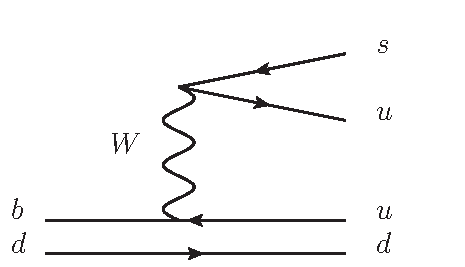
\includegraphics[width=\textwidth]{introduction/weak_tree}
    \caption{Tree diagram}
    \label{fig:intro:sm:weak_feynman:tree}
  \end{subfigure}
  \begin{subfigure}{0.55\textwidth}
    \centering
    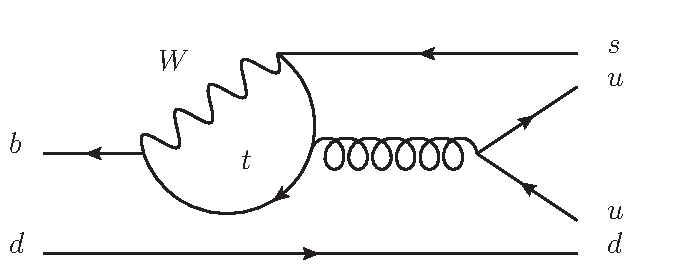
\includegraphics[width=\textwidth]{introduction/weak_penguin}
    \caption{Penguin diagram}
    \label{fig:intro:sm:weak_feynman:penguin}
  \end{subfigure}
  \caption{%
    Two possible Feynman diagrams for the decay \decay{\PBzero}{\PKplus\Ppiminus}.
  }
  \label{fig:intro:sm:weak_feynman}
\end{figure}


\chapter{The \acl{LHC}}
\label{chap:intro:lhc}

As high-energy particle physics has progressed over the last century, the 
meaning of `high energy' has continuously evolved.
Today, high energy refers to the \acl{LHC}~\cite{Bruning:2004ej}, a circular 
collider which began operating at a proton-proton centre of mass energy of 
\sqrtseq{7} in 2010, and in 2015 reached \sqrtseq{13}.
This section will describe the machine, the experiments which it services, and 
the changes in operation throughout its lifetime so far.

In order to produce collisions, bunches of \num{1.2e11} protons are obtained 
through the ionisation of hydrogen gas, and are then accelerated through a 
chain of progressively larger, more powerful accelerators before being injected 
into the \ac{LHC}.
During nominal operation, a single \ac{LHC} `fill' consists of injecting 2808 
bunches into the machine, each of which is about \SI{30}{\centi\metre} long, 
separated from the surrounding bunches by about \SI{7}{\metre}, completing a 
full revolution of the ring at a rate of \SI{11.246}{\kilo\hertz}.

The beams are steered around the ring by superconducting dipole magnets, cooled 
to \SI{1.9}{\kelvin}, and are focused by quadrupole and other, higher-order, 
magnets.
The beams are made to collide at four \acp{LHCIP}, before which they are 
focused further, from the usual circulating bunch diameter of 
\SI{0.2}{\milli\metre} to a width on the order of microns, such that they can 
collide.

For a collision experiment, the rate $N$ at which a particular process occurs 
per second is given by
\begin{equation}
  N = \lumi\xsec,
  \label{eqn:intro:lhc:lumi_xsec}
\end{equation}
where \lumi\ is the instantaneous luminosity of the accelerator and \xsec\ is 
the cross-section of the process.
At $\sqrts = \SI{13}{\TeV}$, the visible proton-proton interaction 
cross-section is around $\xsecppvis = 
\SI{70}{\milli\barn}$~\cite{Aaboud:2016mmw,CMS:2016ael}.
Given that this number is fixed by the beam energy and colliding particle type, 
the \ac{LHC} is designed to maximise the luminosity \lumi, which can be 
expressed as
\begin{equation}
  \lumi = \frac{N_{\text{p}}^{2}N_{\text{b}}\revfreq\gamma}{4\pi\epsilon\beta^{*}}F,
  \label{eqn:intro:lhc:inst_lumi}
\end{equation}
where $N_{\text{p}}$ is the number of particles per bunch; $N_{\text{b}}$ is 
the number of bunches per beam; \revfreq\ is the bunch revolution frequency; 
$\gamma$ is the Lorentz factor; $\epsilon$ is the beam emittance during 
circulation, a measure of the beam size transverse to the beam direction; 
$\beta^{*}$ is a measure of the transverse beam size at a particular 
\ac{LHCIP}; and $F$ accounts for non-zero crossing angles between the two beams 
at an \ac{LHCIP}.
Depending on the experiment, the \betastar\ parameter can be tuned to provide a 
specific average number $\nu$ of collisions per bunch crossing.
The design luminosity at the \atlas\ and \cms\ \acp{LHCIP} is
\SI{1e34}{\per\square\centi\metre\per\second}, which results in a rate of 
visible proton-proton interactions of \SI{700}{\mega\hertz}.

\subsection{Running periods}

The \ac{LHC} first began running in 2010 at a proton-proton centre-of-mass 
energy of $\sqrts = \SI{7}{\TeV}$, and this continued until the end of 2011.
In 2012, the centre-of-mass energy was increased to $\sqrts = \SI{8}{\TeV}$, 
before the machine was shut down at the end of 2012.
This marked the end of \runone\ and the beginning of \acf{LS1}, during which 
the accelerator was upgraded in order to prepare the machine for running at 
$\sqrts = \SI{13}{\TeV}$.
This new phase of operation, \runtwo, began in mid-2015, and is expected to 
continue until the end of 2018.


\chapter{The \lhcb\ experiment}
\label{chap:intro:lhcb}

The \lhcb\ experiment comprises a collaboration of around one thousand 
scientists and engineers, and a particle detector situated at point 8 of the 
\cern\ \ac{LHC}.
The general goal of the experiment is to explore the area of \emph{heavy 
  flavour physics}, that is the interactions of charm and beauty quarks and 
particles that contain them.
Specific aims will be given in \cref{chap:intro:lhcb:physics}, and the design 
and construction of the detector will be described in 
\cref{chap:intro:lhcb:detector}.
First, a brief introduction to the mechanisms of a high-energy particle physics 
experiment will be given, such that the particular requirements of a heavy 
flavour experiment can be related to the design of a detector.

Heavy flavour hadrons, such as the \PBs meson, have short lifetimes, and do not 
fly far enough to interact with active elements of a detector before decaying.
By the studying the properties of decay products with longer lifetimes, the 
properties of the unseen heavy flavour hadrons can be inferred, to be compared 
with those predicted by the \ac{SM}.
% Such properties include production and decay rates, lifetimes, and masses.

The momentum four-vector $\fvec{p}$ of a particle is defined by three spatial 
components, equal to components of the momentum three-vector $\vec{p}$, and the 
energy $E$
\begin{equation}
  \fvec{p} = \begin{pmatrix}E\\\vec{p}\end{pmatrix}
           = \begin{pmatrix}E\\p_{x}\\p_{y}\\p_{z}\end{pmatrix}.
  \label{intro:lhcb:four_momentum}
\end{equation}
Both the energy and the momentum can be measured, using techniques which will 
be discussed later.
The mass of every massive particle is unique, and so by knowing the 
four-momentum of a particle, one implicitly knows its identity by knowing the 
mass using the relation
% The energy can either be measured directly, using methods discussed later, or 
% computed using an assumed mass \mass\ and the magnitude of the measured 
% momentum three-vector $\ptot = |\vec{p}|$
\begin{equation}
  E = \sqrt{p^{2} + m^{2}}.
  \label{intro:lhcb:energy}
\end{equation}
To compute the four-momentum of a heavy flavour hadron, in order to know its 
identity, one can sum the four-momenta of the decay products
\begin{equation}
  \fvec{p}_{\text{Parent}} = \sum_{\text{Children}} \fvec{p}_{i}.
  \label{intro:lhcb:four_momentum_sum}
\end{equation}
It is then the task of the experiment to measure the three-momentum and energy 
of all the decay products in order to study heavy flavour.

\subsection{Momentum measurements}

Particles with lifetimes much greater than those of heavy flavour hadrons, such 
as muons, kaons, pions, and protons (denoted \Pmupm, \PKpm, \Ppipm, and 
\Pproton/\APproton), can pass through several layers of active detector 
elements.
The elements can be ionised by the passage of the charged particles, and this 
can be converted into electrical signals.
By studying the geometric pattern of these `hits', one can reconstruct the 
physical path, or `track', the particle made as it travelled through the 
detector.
The set of detector elements used to measure hits is called the tracking 
system.
To measure the three-momentum of the particles, a magnetic field can be applied 
across their path, as shown in \cref{fig:intro:lhcb:tracking}, causing them to 
bend in a circular arc due to the Lorentz force
\begin{equation}
  \vec{F} = q\vec{v}\times\vec{B}
          = \frac{q}{m}\vec{p}\times\vec{B},
  \label{eqn:intro:lhcb:lorentz_force}
\end{equation}
where $\vec{v}$ is the particle velocity three-vector, $q$ is the electric 
charge of the particle, $m$ is its invariant mass, and $\vec{B}$ is the 
magnetic field vector.
As the direction of the particle is already known from the track 
reconstruction, the coordinate system can be aligned such that the magnetic 
field is perpendicular to the momentum direction.
\Cref{eqn:intro:lhcb:lorentz_force} then reduces to a scalar equation for the 
force magnitude $F$, and can be equated to the centripetal force
\begin{equation}
  F = \frac{q}{m}pB = \frac{mv^{2}}{r},
  \label{eqn:intro:lhcb:lorentz_centripetal}
\end{equation}
where $r$ is the radius of the circular path the charged particle will follow 
in the magnetic field.
The momentum can then be computed as
\begin{equation}
  p = qrB.
  \label{eqn:intro:lhcb:momentum_from_magnet}
\end{equation}
In this coordinate system, positively charged particles will bend in a plane in 
the opposite direction to negatively charged particles, and so the `charge' of 
a track can be deduced by observing in which direction it bends in the magnetic 
field.
Neutral particles do not leave hits in the tracking system, and so, as there 
are no known long-lived particles with $q \geq 2$, the magnitude is assumed to 
be 1.

For a given magnetic field strength $B$, higher momentum particles will bend 
less, to the point where the tracking system is not precise enough to be able 
to measure the bending radius, and hence the momentum.
Particles with a low enough momentum will be bent out of the detector entirely.
For a given tracking system, larger bending radii will lead to more precise 
momentum measurements, and so there is a balance between the momentum range a 
detector is able to measure, and the precision to which those measurements can 
be made.

\begin{figure}
  \centering
  \begin{tikzpicture}[
  x={(0.866cm, -0.5cm)}, y={(0.866cm, 0.5cm)}, z={(0cm, 1cm)},
  scale=0.9,
  inner sep=0pt, outer sep=2pt,
  axis/.style={thick,->},
  station/.style={fill=black!40!white, opacity=0.3},
  particle/.style={->, dashed},
  hit/.style={star,star points=7,draw=black!70,fill=red!70,inner sep=0pt,minimum size=0.2cm}
  ]

  % Coordinate axes
  \coordinate (O) at (0, 0, 0);
  \draw[axis] (O) -- +(14, 0, 0) node [right] {$z$};
  \draw[axis] (O) -- +(0, 2.5, 0) node [right] {$x$};
  \draw[axis] (O) -- +(0, 0, 2) node [left] {$y$};

  % Upstream tracking stations
  \filldraw[station] (1, -2, -1.5) -- (1, -2, 1.5) -- (1, 2, 1.5) -- (1, 2, -1.5) -- (1, -2, -1.5);
  \filldraw[station] (2, -2, -1.5) -- (2, -2, 1.5) -- (2, 2, 1.5) -- (2, 2, -1.5) -- (2, -2, -1.5);
  \filldraw[station] (3, -2, -1.5) -- (3, -2, 1.5) -- (3, 2, 1.5) -- (3, 2, -1.5) -- (3, -2, -1.5);
  % Downstream tracking stations
  \filldraw[station] (8, -2, -1.5) -- (8, -2, 1.5) -- (8, 2, 1.5) -- (8, 2, -1.5) -- (8, -2, -1.5);
  \filldraw[station] (9, -2, -1.5) -- (9, -2, 1.5) -- (9, 2, 1.5) -- (9, 2, -1.5) -- (9, -2, -1.5);
  \filldraw[station] (10, -2, -1.5) -- (10, -2, 1.5) -- (10, 2, 1.5) -- (10, 2, -1.5) -- (10, -2, -1.5) node [below, sloped, near end] {\tiny{Tracking station}};

  % Muons
  \draw[particle] plot [smooth] coordinates {(O) (5.5, 0, 1.5) (13, 0, 0.5)} node [right] {$\mu^{-}$};
  \draw[particle] plot [smooth] coordinates {(O) (4.5, 0, -1.5) (13, 0, -1.0)} node [right] {$\mu^{+}$};

  % Hits
  % Negative muon at upstream stations
  \node[hit] at (1, 0, 0.3) {};
  \node[hit] at (1.1, 0, 0.4) {};
  \node[hit] at (3, 0, 0.9) {};
  \node[hit] at (3, 0, 1.0) {};
  \node[hit] at (4.5, 0, 1.5) {};
  \node[hit] at (4.3, 0, 1.3) {};
  \node[hit] at (4.4, 0, 1.3) {};
  % Negative muon at downstream stations
  \node[hit] at (8, 0, 1.2) {};
  \node[hit] at (8.1, 0, 1.4) {};
  % \node[hit] at (9.2, 0, 1.1) {};
  \node[hit] at (9.3, 0, 1.0) {};
  \node[hit] at (11.5, 0, 0.8) {};
  \node[hit] at (11.3, 0, 0.8) {};
  \node[hit] at (11.4, 0, 0.9) {};

  % Magnetic field vector
  \draw[thick,->] (5, 2, 1.5) -- (5, 2, 1.0) node [anchor=west] {$\vec{B}$ field} -- (5, 2, 0.5);
\end{tikzpicture}

  \caption{%
    Illustration of particle tracking, showing two muons traversing through a 
    series of tracking stations, with a magnetic field in the negative $y$ 
    direction, bending charged particles in the $xz$ plane.
    Hits made by the negatively charged muon are shown as red points.
    The scatter the hits around the true particle trajectory signifies the 
    inherent uncertainty in the experimental measurement.
  }
  \label{fig:intro:lhcb:tracking}
\end{figure}

\subsection{Energy measurements}

With the momentum three-vector measured with the tracking system, the energy 
$E$ is left as an unknown.
This can be measured using a calorimeter.
The ionisation of the tracking system discussed previously requires a small 
amount of energy, which is lost from the particle traversing the detector.
A calorimeter takes this process to its limit, being designed to absorb 
particles completely, converting their kinetic energy into a measurable form.
The incident particles lose their energy via particle showers, where 
interactions with the detector material creates additional, lower energy 
particles, and those particles traverse the detector, interact, and create 
further particles with lower energy still.

Calorimeters are placed after the tracking system, as most particles are fully 
absorbed into them, making further measurements of their properties impossible.
Also in contrast to the tracking system, calorimeters can be used to measure 
both neutral and charged particles, and usually a series of individual 
calorimeters is placed one after the other in order to measure different 
particle types in turn, which interact differently with the detector.
Electrons and photons deposit their energy via electromagnetic showers, which 
form due to two processes: high-energy electrons emit photons via 
\emph{bremsstrahlung}; and high-energy photons convert into electron-positron 
pairs.
These two processes alternate back and forth, with $\Pelectron\APelectron$ 
pairs emitting bremsstrahlung photons, which in turn convert into 
$\Pelectron\APelectron$ pairs.
Hadrons, such as protons and charged and neutral pions, produce hadronic 
showers, where the energy loss is due to several processes.
Nuclear interactions, where the hadrons collide with the nuclei in the 
detector, produce additional particles which in turn undergo nuclear 
interactions, creating a cascade.
Hadrons created in this cascade can include \Ppizero and \Peta mesons, which 
decay primarily to final states comprised of electron and photons, and hence 
electromagnetic showers are also created.
The final states of the decays of other particles can include muons and 
neutrinos, which can traverse the calorimeter without interacting further, 
resulting in missing energy.
The length at which electromagnetic and hadronic interactions occur is 
characterised by the interaction lengths \radlen\ and \hadlen\ respectively, 
which depends on the density of the material.
For a given density the hadronic interaction length is much larger than the 
electromagnetic, $\radlen \gg \hadlen$, and so typically an electromagnetic 
calorimeter is placed before a hadronic calorimeter in an experiment, such that 
the electron and photon energies can be measured independently of the hadron 
energies.

The \emph{active} elements of a calorimeter are the materials which converts 
the deposited energy of the particles showers into some measurable quantity, 
either electric charge or light.
The amount of charge or light produced relates to the energy deposited.
The \emph{absorber} elements of a calorimeter are high-density materials that 
reduce the kinematic energy of the incident particles and provide the bulk of 
interaction length.
Homogeneous calorimeters are made solely from active materials, whereas 
sampling calorimeters are constructed from alternating layers of active and 
absorber elements.
Homogeneous calorimeters provide the most accurate measurements, as the entire 
energy deposit can be measured, whereas in a sampling calorimeter some fraction 
is lost to the absorber elements and must be estimated.
The disadvantage of using active elements exclusively is that the suitable 
materials are less dense that the those available solely for absorption, and so 
a larger detector is required for a given energy range that is to be measured.
In practice, hadronic calorimeters are almost exclusively of the sampling type.

\subsection{Particle identification}

If the momentum and energy can be measured precisely, the mass of the particle 
can be deduced with \cref{intro:lhcb:energy}, and hence the particle's identity 
can be known.
As the momentum and energy measurements are subject to experimental resolution, 
there is an uncertainty on the mass measurement.
Alternative \ac{PID} methods are often employed improve this precision.

For charged particles, a measurement of the momentum from the tracking system 
can be combined with a measurement of the velocity to determine the mass from 
the relation $\ptot = \mass\beta\gamma c$.
As $\gamma$ is a function only of $\beta$, as in 
\cref{eqn:intro:sm:lorentz_factor}, and $\beta = v/c$, only one of $\gamma$ and 
$\beta$ needs to be measured.

One method for measuring $\beta$ is to measure the time taken for the particle 
to travel between two detectors.
The measured time difference between detection times $t_{1}$ and $t_{2}$ is 
equal to the distance between the two detectors $L$ divided by the particle 
velocity
\begin{equation}
  \delta t = t_{1} - t_{2} = \frac{L}{v}
           = \frac{L}{\beta c}.
\end{equation}
For a given momentum \ptot, particles with different masses will have different 
velocities, and hence different $\beta$ factors.
In the ultra-relativistic limit, where $pc \gg mc^{2}$, the difference between 
times for two particles with masses $m_{a}$ and $m_{b}$ will be
\begin{equation}
  \Delta t = \delta t_{a} - \delta t_{b}
           \approx \frac{Lc}{2p^{2}}(m_{a}^{2} - m_{b}^{2}),
\end{equation}
The utility of such a technique reduces as the particle momentum increases, as 
a very high precision is required on the time difference measurement in order 
to be able to distinguish between different particle species.

Another \ac{PID} technique is to exploit the phenomenon of Cherenkov radiation, 
where charged particles emit light when they traverse a medium at faster than 
the phase velocity of light in that medium.
The phase velocity of light, or just `the speed of light', in a medium with a 
refractive index $n$ is
\begin{equation}
  v_{\text{Light}} = \frac{c}{n}.
\end{equation}
A front of Cherenkov light is emitted at an angle \cherenkovangle\ to the 
trajectory of the particle, and this angle is related to the speed of light in 
the medium and the velocity magnitude of the particle
\begin{equation}
  \cos{\cherenkovangle} = \frac{v_{\text{Light}}}{v_{\text{Particle}}}
                        = \frac{c}{n\beta c}
                        = \frac{1}{n\beta},
\end{equation}
as illustrated in \cref{fig:intro:lhcb:cherenkov}.
Given that the medium is chosen by the experimenter, so that $n$ is known, 
$\beta$ can be measured by measuring the angle of the Cherenkov light.
As in the time-of-flight method, different particle species with the same 
measured momentum will have different values of $\beta$, and in this case 
different angles \cherenkovangle.
Unlike the time-of-flight method, which requires high temporal resolution to 
distinguish particle hypotheses, the Cherenkov methods requires high spatial 
resolution, so that different ring sizes can be measured.
TODO: talk quantitatively about the precision, as in the time-of-flight example.

% TODO: discuss muon ID
% Muons are special because they punch through everything easily, so one method 
% for ID'ing them is just to have an additional tracking system after the calo

The techniques which have been discussed for measuring particle momentum, 
energy, and identity are general.
The technologies used to construct an experiment depend on the physics that 
experiment intends to measure.

\begin{figure}
  \centering
  \begin{tikzpicture}
  \coordinate (O) at (0, 0);
  \pgfmathsetmacro{\ringbeginx}{5};
  \pgfmathsetmacro{\ringradius}{2};

  % Momentum vector
  \draw[-latex] ($(O) - (0.5, 0)$) -- (O) -- (\ringbeginx, 0) -- +(1, 0) node [anchor=west] {\ptot};

  % Cherenkov light
  \draw[dashed] (O) -- +(\ringbeginx, \ringradius) node [pos=0.5, anchor=south east] {$\frac{c}{n}t$};
  \draw[dashed] (O) -- +(\ringbeginx, -\ringradius);
  \draw (1, 0) arc (0:22:1);
  \node at (10:1.25)  {{\footnotesize $\theta_{c}$}};

  % Projection of light on to detection surface, forming a ring
  \draw[dotted] (\ringbeginx, 0) ellipse (0.1cm and \ringradius cm);
  % Ring radius
  \draw[<->] ($(\ringbeginx, 0) + (0.3, 0)$) -- ($(\ringbeginx, -\ringradius) + (0.3, 0)$) node [pos=0.5, anchor=west] {$R$};

  % Measurement of particle flight distance
  \draw[<->]  ($(O) + (0, -\ringradius) - (0, 0.2)$) -- ($(\ringbeginx, -\ringradius) - (0, 0.2)$) node [pos=0.5, anchor=south] {$\beta ct$};
\end{tikzpicture}

  \caption{%
    Illustration of Cherenkov light being emitted from a particle travelling 
    with momentum $p$ and velocity $\beta$ through a medium with refractive 
    index $n$.
    The radiation is emitted at a angle \cherenkovangle\ to the trajectory of 
    the particle, and forms a ring of radius $R$ when projected onto a plane 
    transverse to the particle momentum direction.
  }
  \label{fig:intro:lhcb:cherenkov}
\end{figure}

\section{Physics goals}
\label{chap:intro:lhcb:physics}

% TODO in order of importance:
% heavy flavour at LHC is forward -> detector is forward
% heavy flavour travels measurable distance -> measure it
% heavy flavour decays to hadrons -> PID

% Measure properties of HF
%   * Lifetimes
%   * Masses
%   * CP violation observables
%   * Production rates

The \lhcb\ experiment aims to make the most precise measurements of heavy 
flavour properties to date, and to discover decays that were not observed by 
previous experiments.
This section will link the properties of heavy flavour decays with the 
requirements imposed on the detector if one wants to study those properties.

As discussed previously, the properties of short-lived heavy flavour hadrons 
can be inferred by reconstructing the four-momenta of their decay products, and 
so \lhcb\ aims to fully reconstruct the decays of beauty and charm hadrons, 
such as $\decay{\PBz}{\PKplus\PKminus}$, $\decay{\PBs}{\PDspm\PKmp}$ with 
$\decay{\PDsplus}{\PKminus\PKplus\Ppiplus}$, 
$\decay{\PLambdab}{\PJpsi\Pproton\PKminus}$ with 
$\decay{\PJpsi}{\Pmuon\APmuon}$, and $\decay{\PDz}{\PKplus\Ppiminus}$.
It is important to note that specific final states offer higher sensitivities 
to physics observables than others, and so it is crucial for \lhcb\ to be able 
to distinguish between different particle species.
For example, the decay $\decay{\PDz}{\PKplus\Ppiminus}$ is of the order of one 
thousand times less likely than the decay $\decay{\PDz}{\PKminus\Ppiminus}$, 
and so a poor \ac{PID} performance would result in a search for the 
$\PKplus\Ppiminus$ final state being swamped by $\PKminus\Ppiplus$.

The short lifetime of heavy flavour hadrons can be exploited to reduce 
background.
In general, tens to hundreds of particles are produced per proton-proton 
interaction, only one or two of which may be the signal particle of interest.
Most of the background particles will be pions, kaons, and protons, which are 
long lived an will fly through the tracking system, with their reconstructed 
tracks pointing back to the proton-proton interaction region, called the 
\ac{PV}.
As the heavy flavour hadrons are much lighter than the centre-of-mass energy of 
the colliding beams, with the \PBz meson having a mass of \SI{5.28}{\GeV} and 
the \PDz meson having a mass of \SI{1.86}{\GeV}, they have a large boost in the 
laboratory frame, greatly increasing their lifetime, in accordance with 
\cref{eqn:intro:sm:lifetime_lab}.
Heavy flavour hadrons can then fly millimetres in the laboratory frame before 
decaying, and a displaced decay vertex can then be reconstructed by combining 
tracks that intersect.
Particles produced in decays displaced from the \ac{PV} will have tracks which, 
in general, does not point back to the \ac{PV}.
This is illustrated in \cref{fig:intro:lhcb:vertexing}, showing the 
\emph{impact parameter}, the smallest perpendicular distance from the track to 
the \ac{PV}.
Particles produced directly in the proton-proton interaction will have a small 
\ac{IP}, whereas those produced in \emph{secondary decays}, from heavy flavour 
hadrons, will in general have large \acp{IP}.
Being able to measure both the degree to which a decay vertex is displaced from 
the \ac{PV} and the \acl{IP} of tracks with a high precision would then allow 
for discrimination between signal and background.

Precision is driven by the amount of data that is collected, and so the 
experiment aims to maximise this.
At the \ac{LHC}, the primary interaction mechanism between proton-proton 
bunches is gluon-gluon fusion, as in 
\cref{fig:intro:lhcb:hf_production:gg_fusion}, and with this mechanism \bbbar\ 
and \ccbar\ pairs are predominantly produced in the \emph{forward} region, as 
shown in \cref{fig:intro:lhcb:hf_production:bbbar_angles}.
Instrumenting this region is then beneficial to collect large samples of heavy 
flavour, however it comes with a price.

\begin{figure}
  \begin{subfigure}[b]{0.4\textwidth}
    \centering
    \feynmandiagram [large, horizontal=a to b] {%
  i1 [particle=\(\Pgluon\)] -- [gluon] a -- [gluon] i2 [particle=\(\Pgluon\)],
  a -- [gluon, edge label=\(\Pgluon\)] b,
  f1 [particle=\(\APquark\)] -- [fermion] b -- [fermion] f2 [particle=\(\Pquark\)],
};

    \caption{Quark pair production}
    \label{fig:intro:lhcb:hf_production:gg_fusion}
  \end{subfigure}
  \begin{subfigure}[b]{0.6\textwidth}
    \begin{tikzpicture}
  \node[anchor=south west, inner sep=0] (image) at (0, 0) {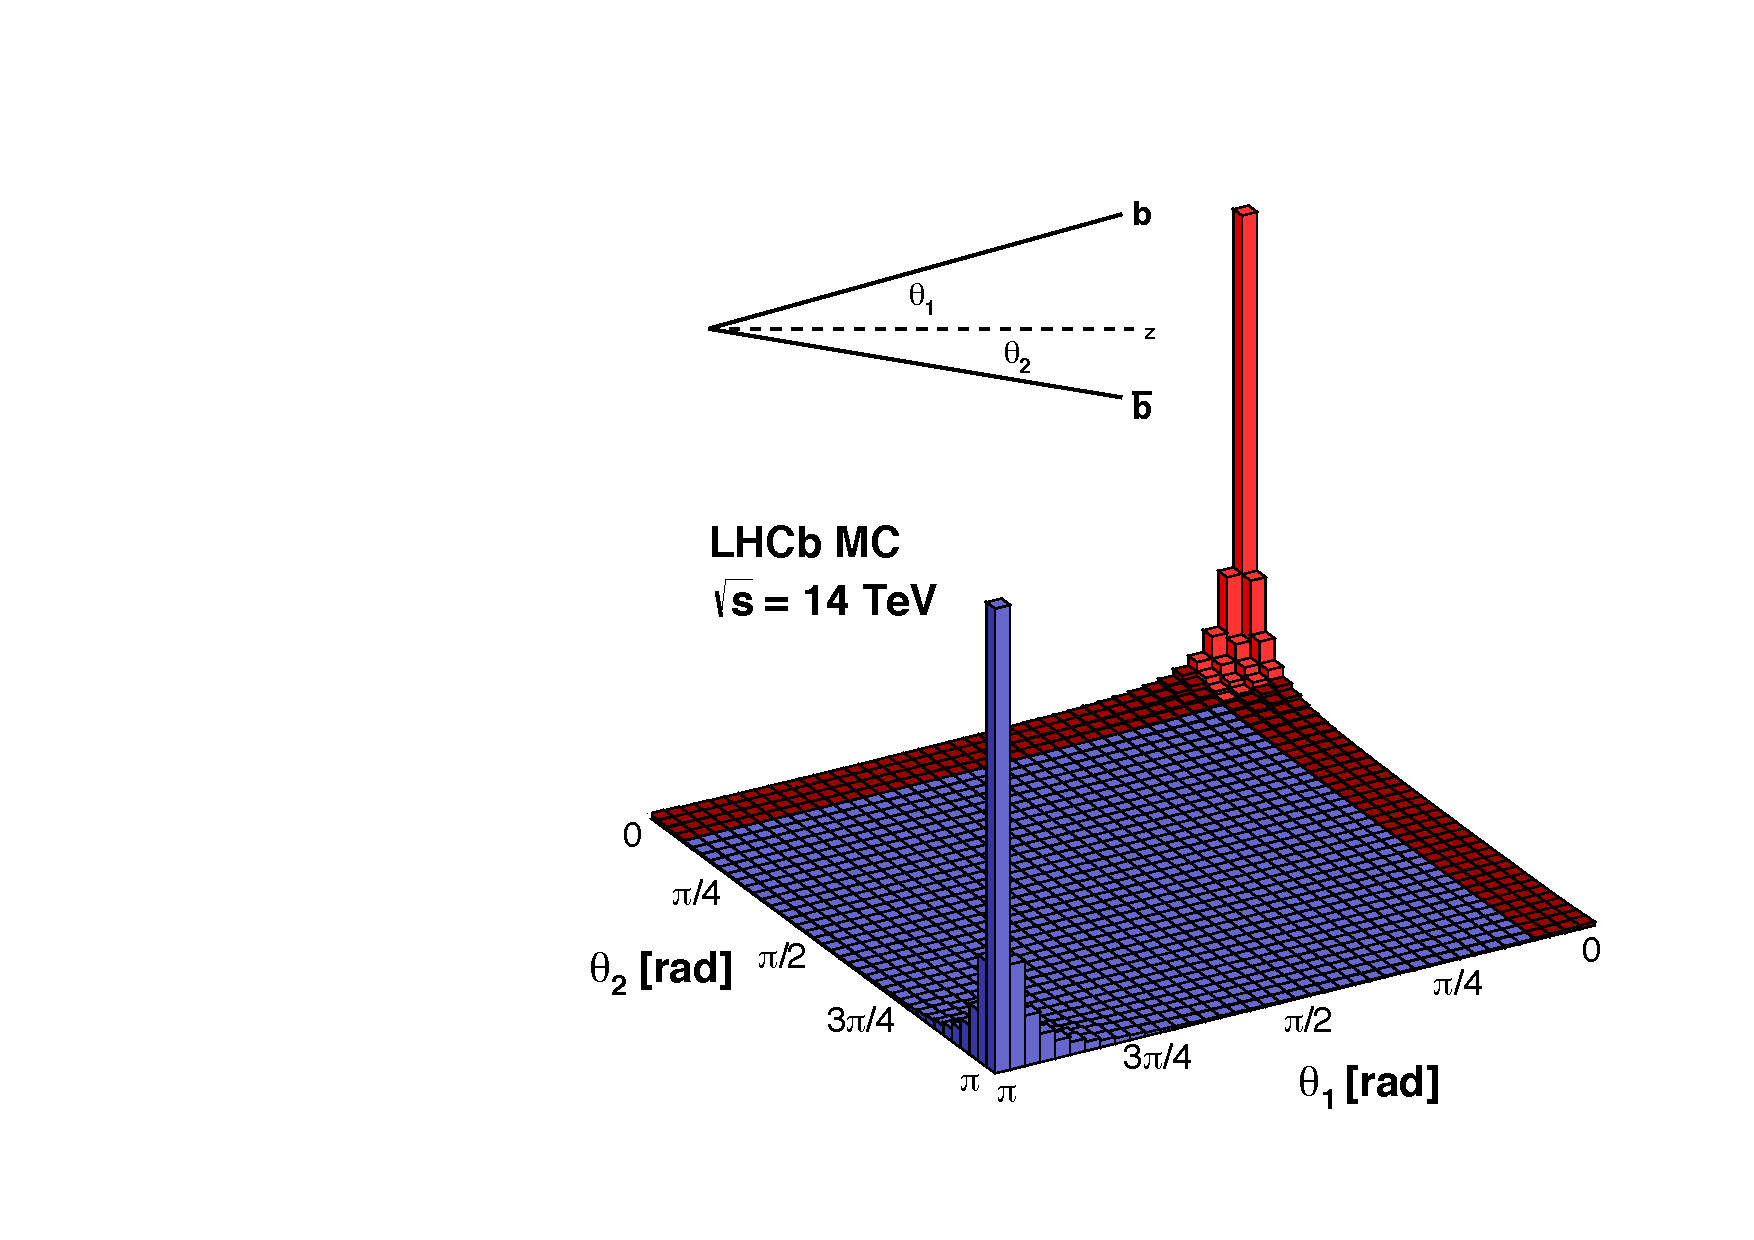
\includegraphics[width=\textwidth]{introduction/bbbar_production_angles}};
  \begin{scope}[x={(image.south east)}, y={(image.north west)}]
    % Grid to help find coordinates on the image
    % \draw[step=0.02, gray, very thin] (0, 0) grid (1, 1);
    % Box to cover axis labels
    \path[fill=white] (0.02, 0.16) rectangle (0.18, 0.22) node [pos=0.5] {\footnotesize$\theta_{1}$};
    \path[fill=white] (0.64, 0.06) rectangle (0.78, 0.12) node [pos=0.5] {\footnotesize$\theta_{2}$};
    % Box to cover angle definitions
    \path[fill=white] (0.14, 0.66) rectangle (0.54, 0.88);
    % Box to cover 'LHCb MC' label
    \path[fill=white] (0.14, 0.48) rectangle (0.36, 0.58);
  \end{scope}
\end{tikzpicture}

    \caption{$\Pbottom\APbottom$ production distribution}
    \label{fig:intro:lhcb:hf_production:bbbar_angles}
  \end{subfigure}
  \caption{%
    Feynman diagram of quark pair production via gluon-gluon fusion 
    (\subref*{fig:intro:lhcb:hf_production:gg_fusion}), and a simulation of the 
    angular distribution of \bbbar\ production at the \ac{LHC} at $\sqrt{s} = 
    \SI{13}{\TeV}$ (\subref*{fig:intro:lhcb:hf_production:bbbar_angles}).
  }
  \label{fig:intro:lhcb:hf_production}
\end{figure}

\begin{figure}
  \centering
  % Draw perpendicular markers at line intersections
% http://tex.stackexchange.com/a/21759/45857
\tikzset{
  right angle quadrant/.code={
    \pgfmathsetmacro\quadranta{{1,1,-1,-1}[#1-1]}     % Arrays for selecting quadrant
    \pgfmathsetmacro\quadrantb{{1,-1,-1,1}[#1-1]}},
  right angle quadrant=1, % Make sure it is set, even if not called explicitly
  right angle length/.code={\def\rightanglelength{#1}},   % Length of symbol
  right angle length=2ex, % Make sure it is set...
  right angle symbol/.style n args={3}{
    insert path={
      let \p0 = ($(#1)!(#3)!(#2)$) in     % Intersection
      let \p1 = ($(\p0)!\quadranta*\rightanglelength!(#3)$), % Point on base line
      \p2 = ($(\p0)!\quadrantb*\rightanglelength!(#2)$) in % Point on perpendicular line
      let \p3 = ($(\p1)+(\p2)-(\p0)$) in  % Corner point of symbol
      (\p1) -- (\p3) -- (\p2)
    }
  }
}
\begin{tikzpicture}[
  x=2cm,
  y=2cm,
  axis/.style={very thick,->,gray},
  beam/.style={very thick,->,gray},
  scale=1.5,
  thick
  ]
  % Origin
  \coordinate (O) at (0, 0);
  % B decay vertex
  \coordinate (Bvtx) at (1, 0.5);
  % Offset of muon arrows, with respect to Bvtx
  \coordinate(mumoffset) at (0.3, 0.4);
  \coordinate(mupoffset) at (0.6, -0.2);
  % Compute the coordinates of the ends of the muon lines
  \coordinate (mum) at ($(Bvtx) + (mumoffset)$);
  \coordinate (mup) at ($(Bvtx) + (mupoffset)$);

  % Coordinate axes
  \draw[axis] (-0.6, -0.5) -- +(0.2, 0) node [below] {$z$};
  \draw[axis] (-0.6, -0.5) -- +(0, 0.2) node [left] {$y$};

  \draw[beam] (-1.0, 0) -- (-0.1, 0) node [below, at start] {$p$};
  \draw[beam] (1.5, 0) -- (0.1, 0) node [below, at start] {$p$};

  % D meson
  \draw[dashed, color=gray, text=black] (O) -- (Bvtx) node [above, pos=0.5] {\PDz};
  % Negative child
  \draw[->] (Bvtx) -- (mum) node [above] {\PKminus};
  \draw[dotted] (Bvtx) -- ($(Bvtx) - 3*(mumoffset)$) node [name=mumend] {};
  % Positive child
  \draw[->] (Bvtx) -- (mup) node [below] {\Ppiplus};
  \draw[dotted] (Bvtx) -- ($(Bvtx) - 2*(mupoffset)$) node [name=mupend] {};

  % Primary vertex
  \node[star,star points=10,draw=orange!50,fill=orange!20,inner sep=0pt,minimum size=0.4cm] at (O) {};

  % Negative muon IP
  \draw[right angle length=1mm, right angle symbol={Bvtx}{mumend}{O}] ($(Bvtx)!(O)!(mumend)$) -- (O) node [pos=0.2, left] {$\text{IP}_{\PKminus}$};
  % Positive muon IP
  \draw[right angle length=1mm, right angle symbol={Bvtx}{mupend}{O}] ($(Bvtx)!(O)!(mupend)$) -- (O) node [midway, left] {$\text{IP}_{\Ppiplus}$};
\end{tikzpicture}

  \caption{%
    Illustration of vertexing, showing a \PDz meson decaying in flight to a 
    kaon and a pion.
    The kaon and pion are reconstructed as tracks, and then \PDz decay vertex 
    is inferred from the point of closest approach of the two tracks.
    The minimum transverse distance the tracks make when extrapolated back 
    towards the primary proton-proton vertex, the \acf{IP}, is shown.
  }
  \label{fig:intro:lhcb:vertexing}
\end{figure}

% The \ac{LHC} provides higher production rates of charm and beauty hadrons that 
% any previous collider, and \lhcb\ is the only dedicated heavy flavour 
% experiment at the \ac{LHC}.
% As such, its primary goal is to study the properties of charm and beauty 
% hadrons, exploiting the large amount of data that has been and continues to 
% made to make precise measurements.

% Unlike \atlas\ and \cms\, the \lhcb\ detector is searching for \ac{BSM} physics 
% primarily through indirect searches.
% The two principle methods in which this is done is through measuring 
% differences between matter and antimatter, and by measuring rare processes such 
% as the \BsTomumu decay.

\section{Detector}
\label{chap:intro:lhcb:detector}

When describing the detector, it is useful to define a common coordinate 
system.
Within the \lhcb\ experiment, it is customary to define a right-handed 
coordinate system, where the $z$-axis is aligned along the beam direction, 
increasing in the clockwise direction along the \ac{LHC} ring; the $y$-axis is 
aligned with gravity, increasing away from the Earth's surface; and the 
$x$-axis, defined as $x = y \times z$, is then increasing away from the centre 
of the accelerator.
In this section, and in all subsequent sections, this coordinate system will be 
used.

The detector is shown in \cref{fig:intro:lhcb:detector}.
How forward a process or a detector is is defined by the polar angle $\theta$, 
defined with respect to the beam, with $0 < \theta < \pi$.
A polar angle close to the extremes is considered forward, whilst values around 
$\sfrac{\pi}{2}$ are \emph{central}.
Another measure is the pseudorapidity
\begin{equation}
  \Eta = -\ln\left(\tan{\frac{\theta}{2}}\right).
  \label{eqn:intro:lhcb:pseudorapidity}
\end{equation}
The pseudorapidity is zero at $\sfrac{\pi}{2}$, and becomes infinite as 
$\theta$ tends to it extremes.
The general purpose \atlas\ and \cms\ detector are instrumented for particle 
tracking in the region $|\Eta| < 2.5$, whereas the \lhcb\ detector is 
instrumented in the region $2 < \Eta < 5$.

\begin{figure}
  \centering
  \begin{tikzpicture}
  % Use trim and crop to remove some of the white space around the image
  \node[anchor=south west, inner sep=0] (image) at (0, 0) {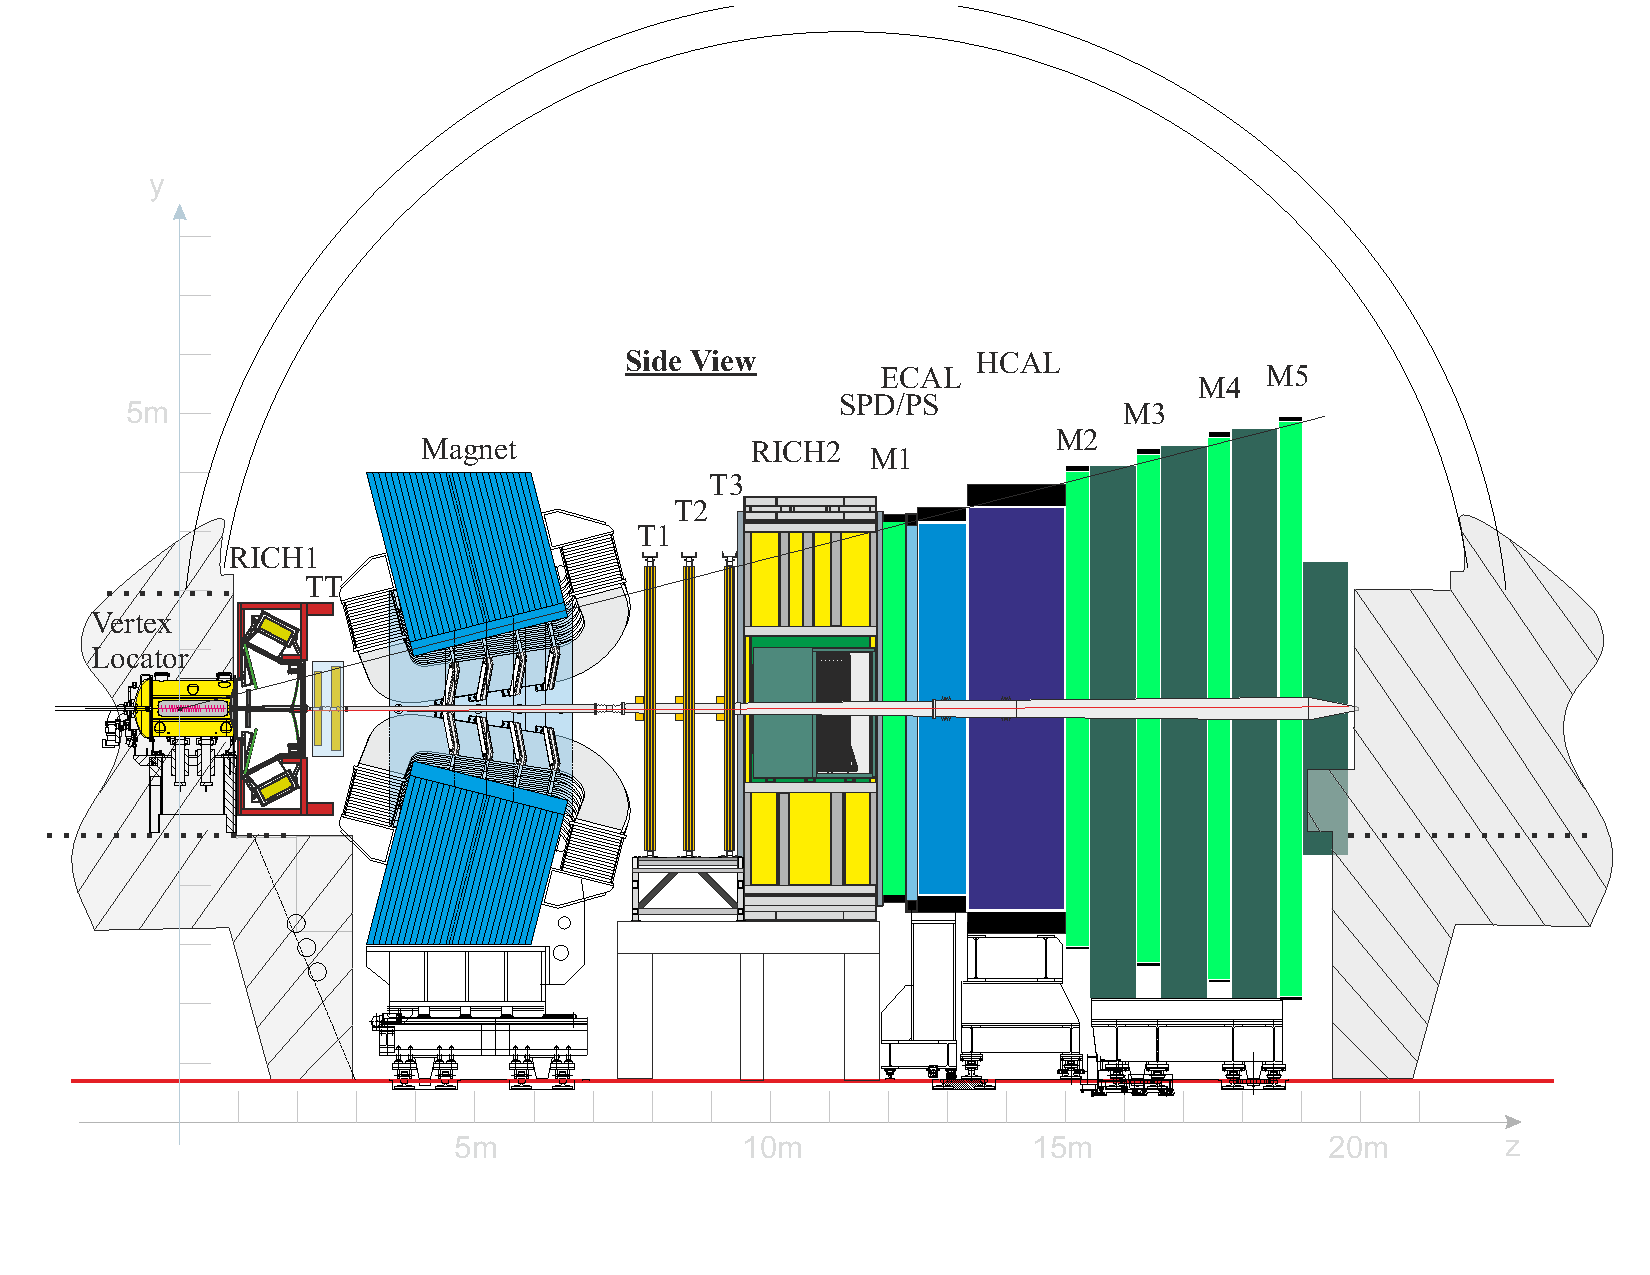
\includegraphics[width=\textwidth, trim={1cm 1.7cm 0.5cm 3cm}, clip]{introduction/lhcb_detector}};
  \begin{scope}[x={(image.south east)}, y={(image.north west)}]
    % Grid to help find coordinates on the image
    % \draw[step=0.02, gray, very thin] (0, 0) grid (1, 1);
    % Box to cover "Side View" label
    \path[fill=white] (0.36, 0.78) rectangle (0.46, 0.84);
  \end{scope}
\end{tikzpicture}

  \caption{%
    A schematic of the \lhcb\ detector.
    In this Figure, the $z$-axis, labelled, increases from left to right, the 
    $y$-axis, also labelled, increases from bottom to top, and the $x$-axis 
    increases into the page.
  }
  \label{fig:intro:lhcb:detector}
\end{figure}

\subsection{Tracking}
\label{chap:intro:lhcb:detector:tracking}

\subsection{Particle identification}
\label{chap:intro:lhcb:detector:pid}

\subsection{Event selection}
\label{chap:intro:lhcb:detector:trigger}

\subsection{Data flow}
\label{chap:intro:lhcb:detector:dataflow}


\part{%
  Charm production
}
\label{chap:prod}

\chapter{Introduction}
\label{chap:prod:introduction}

This \lcnamecref{chap:prod} describes a measurement of charm and \ccbar\ 
production, performed using data taken at $\sqrts = \SI{13}{\TeV}$ with the 
\lhcb\ detector.
At the \ac{LHC}, a given charm hadron \PHc\ can either be produced in the 
proton-proton interaction or in the decays of \PB hadrons.
The latter mechanism is called secondary production, whilst the former is 
called prompt production.
The type of charm hadron produced can either be charmonium, such as the \PJpsi 
meson, or open charm, whose net charm quantum number is non-zero.
This measurement is concerned with the prompt production of open charm hadrons.
Charm hadrons originating from the strong decay of prompt excited charm states 
are also considered to be prompt, and here no attempt is made to distinguish 
between the two sources.

Measurements of \ccbar\ and \bbbar\ cross-sections at the \ac{LHC} are made to 
test the predictions of \ac{QCD}.
The production rate of heavy flavour hadrons is expected to vary as a function 
of hadron \pT\ and rapidity \rapidity, defined as
\begin{equation}
  y = \frac{1}{2}\ln{\frac{E + p_{z}}{E - p_{z}}},
  \label{eqn:prod:introduction:rapidity}
\end{equation}
and so experimental measurements can be compared with both the shape of 
theoretical predictions as a function of \pTy\ as well as to the total 
integrated rate.
Measurements can also be used as inputs to constrain predictions.
Heavy flavour production rates are also used to estimate sensitivities of 
experimental searches for rare decays, and also as inputs to atmospheric 
neutrino experiments, where charm production enters as a background process.

Measuring \ccbar\ and \bbbar\ cross-sections at \lhcb\ is complementary to such 
efforts made using the \acp{GPD}, due to the unique rapidity range of the 
detector, as well as its ability to cleanly reconstruct low \pT\ hadrons.

\section{Analysis overview}
\label{chap:prod:introduction:analysis_overview}

The measured cross-section for the inclusive production of an open charm hadron 
\PHc\ from proton-proton collisions can be expressed as
\begin{equation}
  \xsec(\PHc) = \frac{%
    N(\HcTof)
  }{%
    \eff(\HcTof)\cdot\bfrac(\HcTof)\cdot\intlumi
  },
  \label{eqn:prod:introduction:cross_section}
\end{equation}
where $N(\HcTof)$ is the number of reconstructed and selected prompt charm 
hadrons \PHc\ in some final state $f$; \eff\ is the efficiency of fully 
reconstructing and selecting the decay \HcTof, given that it was produced; 
\bfrac\ is the branching fraction of the decay; and \intlumi\ is the integrated 
luminosity.
To compare with the shapes of theoretical predictions, double differential 
cross-sections can be determined in bins of charm hadron \pT\ and \rapidity, 
using the width $\Delta\pT$ of the bin in \pT\ and the width $\Delta\rapidity$ 
of the bin in rapidity in which the yield and efficiency measurements were made
\begin{equation}
  % There is a "\left." here, which is invisible, to balance the "\right\rvert"
  \left.\frac{\dif^{2}{\xsec(\PHc)}}{\dif{\pT}\dif{\rapidity}}\right\rvert_{i}
    = \frac{1}{\Delta\pT\Delta\rapidity}
      \frac{%
        N_{i}(\HcTof)
      }{%
        \eff_{i}(\HcTof)\cdot\bfrac(\HcTof)\cdot\intlumi
      },
  \label{eqn:prod:introduction:differential_cross_section}
\end{equation}
where $i$ is the index of the \pTy\ bin.

The analysis presented in this \lcnamecref{chap:prod} measures the double 
differential cross-sections of \PDzero, \PDp, \PDsplus, and \PDstarp open charm 
mesons.\footnotemark\
The final states chosen are \DzToKpi, \DpToKpipi, \DspTophipi with \phiToKK, 
and \DstToDzpi with \DzToKpi, the branching fractions of which are listed in 
\cref{tab:prod:introduction:branching_ratios}.
Charge conjugation is implied, in that the cross-sections are measured as the 
combined rate of meson and anti-meson production.
The measurements are made in the \pT\ range \pTrange{0}{15} and the rapidity 
range \yrange{2}{4.5}.
In \rapidity, the measurements are made in five bins of width 0.5, and in \pT\ 
the bins are \SI{1}{\GeVc} in width in the regions \pTrange{0}{1} and 
\pTrange{4}{15}, and are \SI{0.5}{\GeVc} in width in the region \pTrange{1}{4}.

\footnotetext{%
  The excited \PD state is, formally, the \PDstp\ meson, but will be referred 
  to throughout as `\PDstarp'.
}

\begin{table}
  \centering
  \caption{%
      Branching ratios for the different decay 
      modes~\cite{PDG2014,Alexander:2008aa}.
      The \DspTophipi\ branching fraction includes the branching fraction of 
      \phiToKK\@.
  }
  \label{tab:prod:introduction:branching_ratios}
  \begin{tabular}{lS[table-format=1.2(2)]}
  \toprule
  Decay mode  & {\bfrac\ (\si{\percent})} \\
  \midrule
  \DzToKpi    & 3.88 \pm 0.05             \\
  \DpToKpipi  & 9.13 \pm 0.19             \\
  \DspTophipi & 2.24 \pm 0.13             \\
  \DstToDzpi  & 67.7 \pm 0.5              \\
  \bottomrule
\end{tabular}

\end{table}

From the double differential measurements, several derived quantities are 
computed, namely the ratio of charm production rates measured at $\sqrts = 
\SI{13}{\TeV}$ to those measured by \lhcb\ at 
\SI{7}{\TeV}~\cite{LHCb-PAPER-2012-041}, ratios of production rates between 
charm mesons, open charm hadron cross-sections integrated across the \pTy\ 
space, and integrated \ccbar\ cross-sections.
Each integrated per-meson cross-section is the sum over all \pTy\ bins of the 
respective double differential measurements.
The total \ccbar\ cross-sections can be computed using fragmentation fractions, 
each a measurement of the transition probability $f(\cToHc)$ that a charm quark 
will hadronise to a particular open charm hadron.
Given the fragmentation fraction and the integrated cross-section, the 
integrated \ccbar\ cross-section can be computed as
\begin{equation}
  \xsec{(\ccbar)} = \frac{\xsec(\PHc + \APHc)}{2f(\cToHc)}.
  \label{eqn:prod:introduction:ccbar_cross_section}
\end{equation}
The factor $\sfrac{1}{2}$ accounts for the inclusion of the charge conjugate 
(anti-charm) states in the measurement, which have been noted explicitly here 
to avoid ambiguity.
For this analysis, the fragmentation fractions are taken from the 
\ac{PDG}~\cite{PDG2008}, who compute them as averages of measurements made at 
\epem\ colliders operating at a centre-of-mass energy close to the 
\PUpsilonFourS resonance.
These values are given in \cref{tab:prod:introduction:fragmentation_fractions}, 
where the transition probability for \PDzero, $f(\decay{\Pcharm}{\PDzero})$, 
includes contributions from \DstToDzpi\ decays.

\begin{table}
  \caption[Charm hadron fragmentation fractions]{%
    Charm hadron fragmentation fractions~\cite{PDG2008}.
  }
  \label{tab:prod:introduction:fragmentation_fractions}
  \centering
  \begin{tabular}{cc}
  \toprule
  $\PHc$   & $f(\cToHc)$       \\
  \midrule
  \PDz     & $0.565 \pm 0.032$ \\
  \PDp     & $0.246 \pm 0.020$ \\
  \PDsplus & $0.224 \pm 0.028$ \\
  \PDstarp & $0.080 \pm 0.017$ \\
  \bottomrule
\end{tabular}

\end{table}

\subsection{Treatment of uncertainties}
\label{chap:prod:introduction:uncertainties}

Throughout the analysis, the method of \acl{MC} error propagation is used.
With this, each quantity entering 
\cref{eqn:prod:introduction:differential_cross_section} is assumed to be drawn 
from some \acf{PDF} with a known set of parameters, and then ten thousand 
numbers are sampled from that \ac{PDF}.
When performing operations using such quantities, the operations are performed 
on the sample vectors, and then statistics on the result can be computed on the 
new, resulting sample vector.
This technique is used as an analytical error analysis of the measurement is 
complex: what enters into the cross-section is the inverse of the efficiency, 
for example, the corresponding \acl{PDF} of which may not be obvious, in 
particular whether the uncertainties can be treated as Gaussian.
The use of \acl{MC} error propagation simplifies such analyses.

% Don't use pTyrange here as it causes a long, unbroken line
An example cross-section, measured in the region \pTrange{12}{13}, 
\yrange{2.5}{3}, is given in 
\cref{fig::prod:introduction:uncertainties:posterior}.
The blue curve shows the \ac{PDF} of the cross-section, as modelled by the 
\ac{MC} error propagation technique, when only the statistical uncertainty is 
considered, whilst the green curve also includes the contributions from the 
systematic uncertainties.
The green curve is not symmetric, and the mode is shifted with respect to that 
of the blue.

Unless stated otherwise, each quantity that is measured directly is assumed to 
follow a normal distribution, whose mean is equal to the measured value and 
whose width is equal to the measured uncertainty on that value.
The computation of that measured uncertainty will be described when the 
respective quantities are first discussed.
When the results of operations using such inputs are presented, such as 
cross-sections, the central value given is the most probable value of the 
sample vector representing the result, and the lower and upper uncertainty 
bounds are given by the \SI{15.9}{\percent} and \SI{84.1}{\percent} percentiles 
either side of the central value.

\begin{figure}
  \centering
  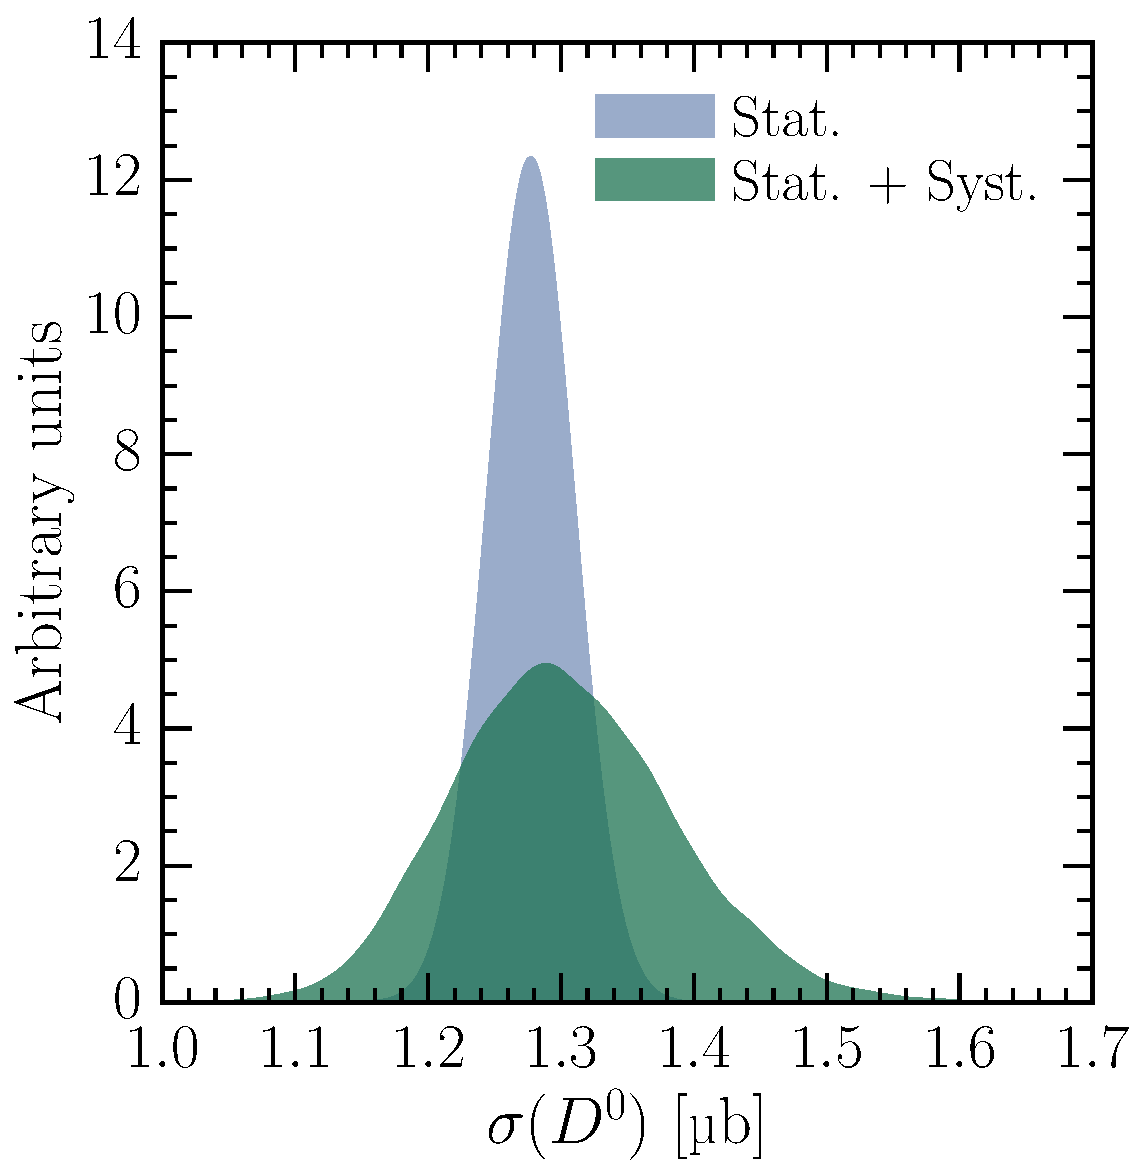
\includegraphics[width=\linewidth]{production/D0ToKpi_posterior_pdf}
  \caption{%
    Posterior probability densities for a measurement of the \PDzero 
    cross-section in the region \pTyrange{12}{13}{2.5}{3}.
    The blue curve shows the density including contributions only from the 
    statistical uncertainty on the prompt signal count.
    The green curve shows the density including contributions from all 
    uncertainties that enter the measurement.
  }
  \label{fig::prod:introduction:uncertainties:posterior}
\end{figure}

\subsection{Document structure}
\label{chap:prod:introduction:structure}

The data used for the measurements were collected in July 2016, under a set of 
special conditions used for the restart of the \ac{LHC} after \ac{LS1}.
The conditions of the \ac{LHC} and of the \lhcb\ detector during this period 
will be described in \cref{chap:prod:data}, along with a description of the 
corresponding simulated data and a summary of the integrated luminosity 
measurement.
The reconstruction and selection of the collected data will be presented in 
\cref{chap:prod:sel}.
The extraction of the prompt charm yields is made on the fully reconstructed 
and selected data using the method of maximum likelihood fits, as described in 
\cref{chap:prod:fitting}.
The evaluation of the associated efficiencies is performed using a mixture of 
simulated \acl{MC} data and dedicated calibration samples, and is discussed in 
\cref{chap:prod:effs}, after which the systematic uncertainties associated with 
all procedures used in the measurement are evaluated, for which the description 
and results are given in \cref{chap:prod:syst}.
Finally, the cross-sections themselves are computed, and are presented in 
\cref{chap:prod:results}.


\chapter{Theory and motivation}
\label{chap:prod:theory}

For an observable cross-section \xsec\ of inclusive production of some object 
$P$, $\decay{h_{A}h_{B}}{PX}$, involving two initial-state hadrons $h_{A}$ and 
$h_{B}$, the dominant contribution to a prediction can be expressed as the 
convolution of several terms
\begin{equation}
  \xsec = \sum_{a,b} \sigma_{a,b} \otimes f_{a,A} \otimes f_{b,B},
  \label{eqn:prod:theory:factorisation}
\end{equation}
where the sum runs over all parton types $a$ and $b$ in the respective hadrons 
$h_{A}$ and $h_{B}$; $\sigma_{a,b}$ is the cross-section of the hard partonic 
interaction $\decay{ab}{PX}$; and $f$ is the \ac{QCDPDF} for the interacting 
parton in the respective hadron~\cite{Collins:1989gx,Forte:2013wc}.
The parton-parton cross-sections $\sigma_{a,b}$, for processes such as heavy 
quark pair production via gluon-gluon fusion shown in 
\cref{fig:intro:lhcb:hf_production:gg_fusion}, can be computed using 
perturbative \ac{QCD}.
The computations of the \acp{QCDPDF} involve low-energy processes below the 
\ac{QCD} scale, and so must be evaluated using non-perturbative \ac{QCD} 
instead.
Clearly, the computation of any cross-section at the \ac{LHC} relies on being 
able to evaluate \cref{eqn:prod:theory:factorisation}, including the 
computation of production rates of the Higgs boson and particles beyond the 
\ac{SM}, and hence on a knowledge of the \acp{QCDPDF}.
As the \acp{PDF} cannot be computed from first principles, they must be derived 
be alternate means, and in practice are constrained using measurements of 
cross-sections by experiments.
Additional measurements of cross-sections can constrain the \acp{QCDPDF} 
further, improving their precision.

Parton density functions are parameterised in terms of \bjorkenx, the fraction 
of the total hadron momentum carried by the interacting parton, and 
\pdfqsquared, a measure of momentum transfer and inversely proportional to the 
spatial `scale' at which the hadron can be probed, with a larger \pdfqsquared\ 
corresponding to a finer resolvable structure.
The \ac{QCDPDF} $f(\bjorkenx, \pdfqsquared)$ for a particular hadron is an 
intrinsic property, and so, for example, experimental measurements that can 
constrain the \ac{QCDPDF} in high-energy proton collisions help not only the 
experiments at that collider, but also experiments at other proton colliders.
This is possible as the evolution of the \acp{QCDPDF} over \pdfqsquared\ for a 
given value of \bjorkenx\ is described by the \ac{DGLAP} differential 
equations~\cite{Gribov:1972ri,Dokshitzer:1977sg,Altarelli:1977zs}.
Measuring a wide range of \bjorkenx\ is important as the individual 
contributions to the total \ac{QCDPDF}, such as from the gluons and the valence 
quarks, vary strongly as a function of \bjorkenx, as shown in 
\cref{fig:prod:theory:pdf_sets}.
The usage of the \ac{DGLAP} equations requires an initial \ac{QCDPDF} from 
which to evolve to different scales, however, as the dependence on \bjorkenx\ 
cannot be computed perturbatively.
Such inputs were first provided by \ac{DIS} experiments, which probe the proton 
structure by colliding leptons and protons.
The subsequent evolution of the \acp{PDF} have been driven by additional 
experimental measurements, and by an improved theoretical understanding of the 
use of the perturbative expansion that must be employed when solving the 
\ac{DGLAP} equations.

The treatment of experimental inputs is a matter of debate, as there are 
somewhat arbitrary choices to be made on what experimental inputs should be 
used, and on how the various experimental uncertainties should be treated.
As a result, different groups of theorists provide so-called `\ac{QCDPDF} 
sets', which differ not only in the treatment of the inputs, but also in the 
treatment of the \emph{theoretical} uncertainties.
These include, for example, the choice of order to which the perturbation 
series are evaluated, and whether the value of the perturbation series scale is 
a parameter of the fit or if it is fixed.
For heavy flavour production, additional uncertainties arise from the choice of 
\emph{fragmentation function} models~\cite{Kneesch:2007ey}, which describe how 
the heavy quarks transition into the observed hadrons, a factor which is not 
included in the factorisation theorem shown in 
\cref{eqn:prod:theory:factorisation}.\footnotemark\
The different \ac{QCDPDF} sets can be used to compute different cross-section 
predictions, and so further experimental measurements can help to distinguish 
between predictions.

\footnotetext{%
  The fragmentation functions are generally assumed to be process independent, 
  e.g.\ they are the same for heavy flavour hadron production from \qqbar\ 
  production at both $\Pelectron\APelectron$ and $\Pproton\Pproton$ colliders.
  They cannot be computed perturbatively, and are extracted from experimental 
  measurements.
}

\begin{figure}
  \begin{subfigure}[b]{0.5\textwidth}
    \centering
    \begin{tikzpicture}
  \node[anchor=south west, inner sep=0] (image) at (0, 0) {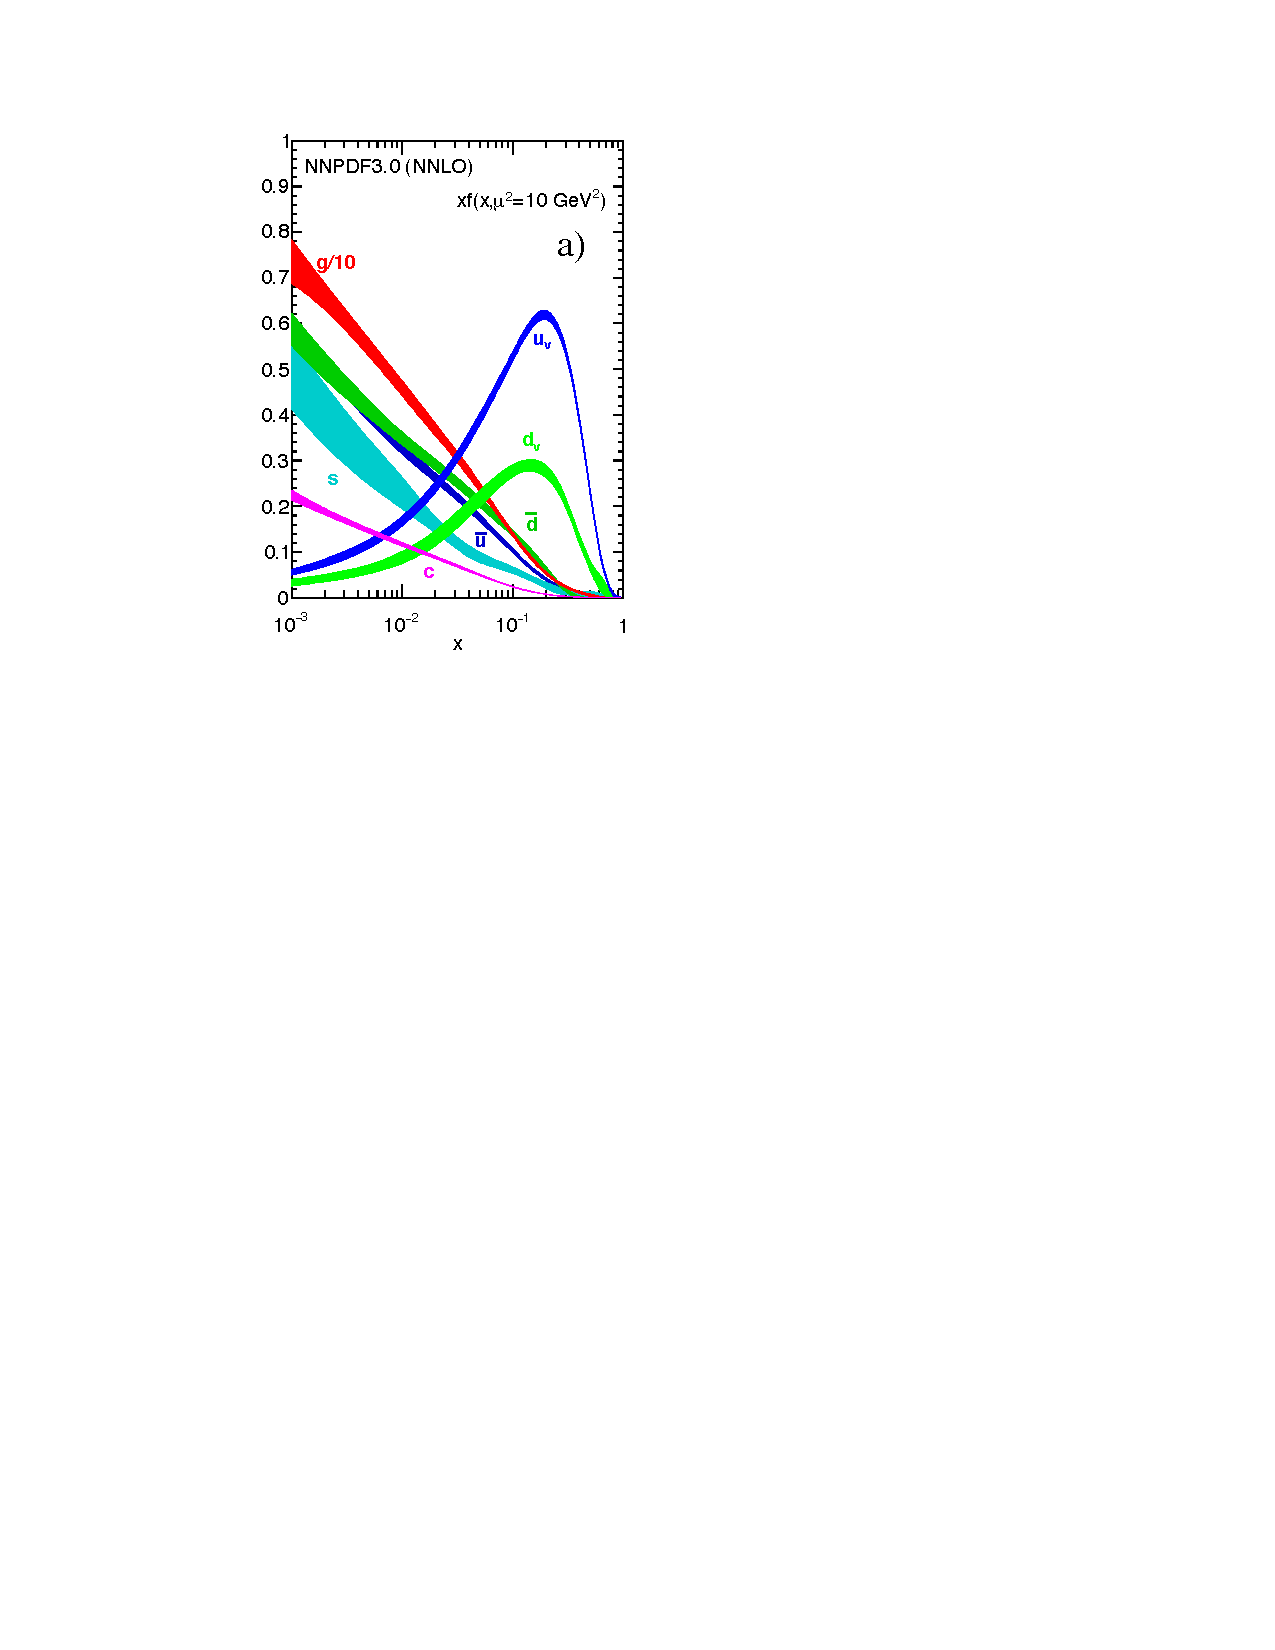
\includegraphics[width=\textwidth]{production/pdf_sets_low_qsquared}};
  \begin{scope}[x={(image.south east)}, y={(image.north west)}]
    % Grid to help find coordinates on the image
    % \draw[step=0.02, gray, very thin] (0, 0) grid (1, 1);
    % Box to cover 'a)' label
    \path[fill=white] (0.8, 0.74) rectangle (0.9, 0.82);
  \end{scope}
\end{tikzpicture}

    \caption{Low \pdfqsquared}
    \label{fig:prod:theory:pdf_sets:low_qsquared}
  \end{subfigure}
  \begin{subfigure}[b]{0.5\textwidth}
    \centering
    \begin{tikzpicture}
  \node[anchor=south west, inner sep=0] (image) at (0, 0) {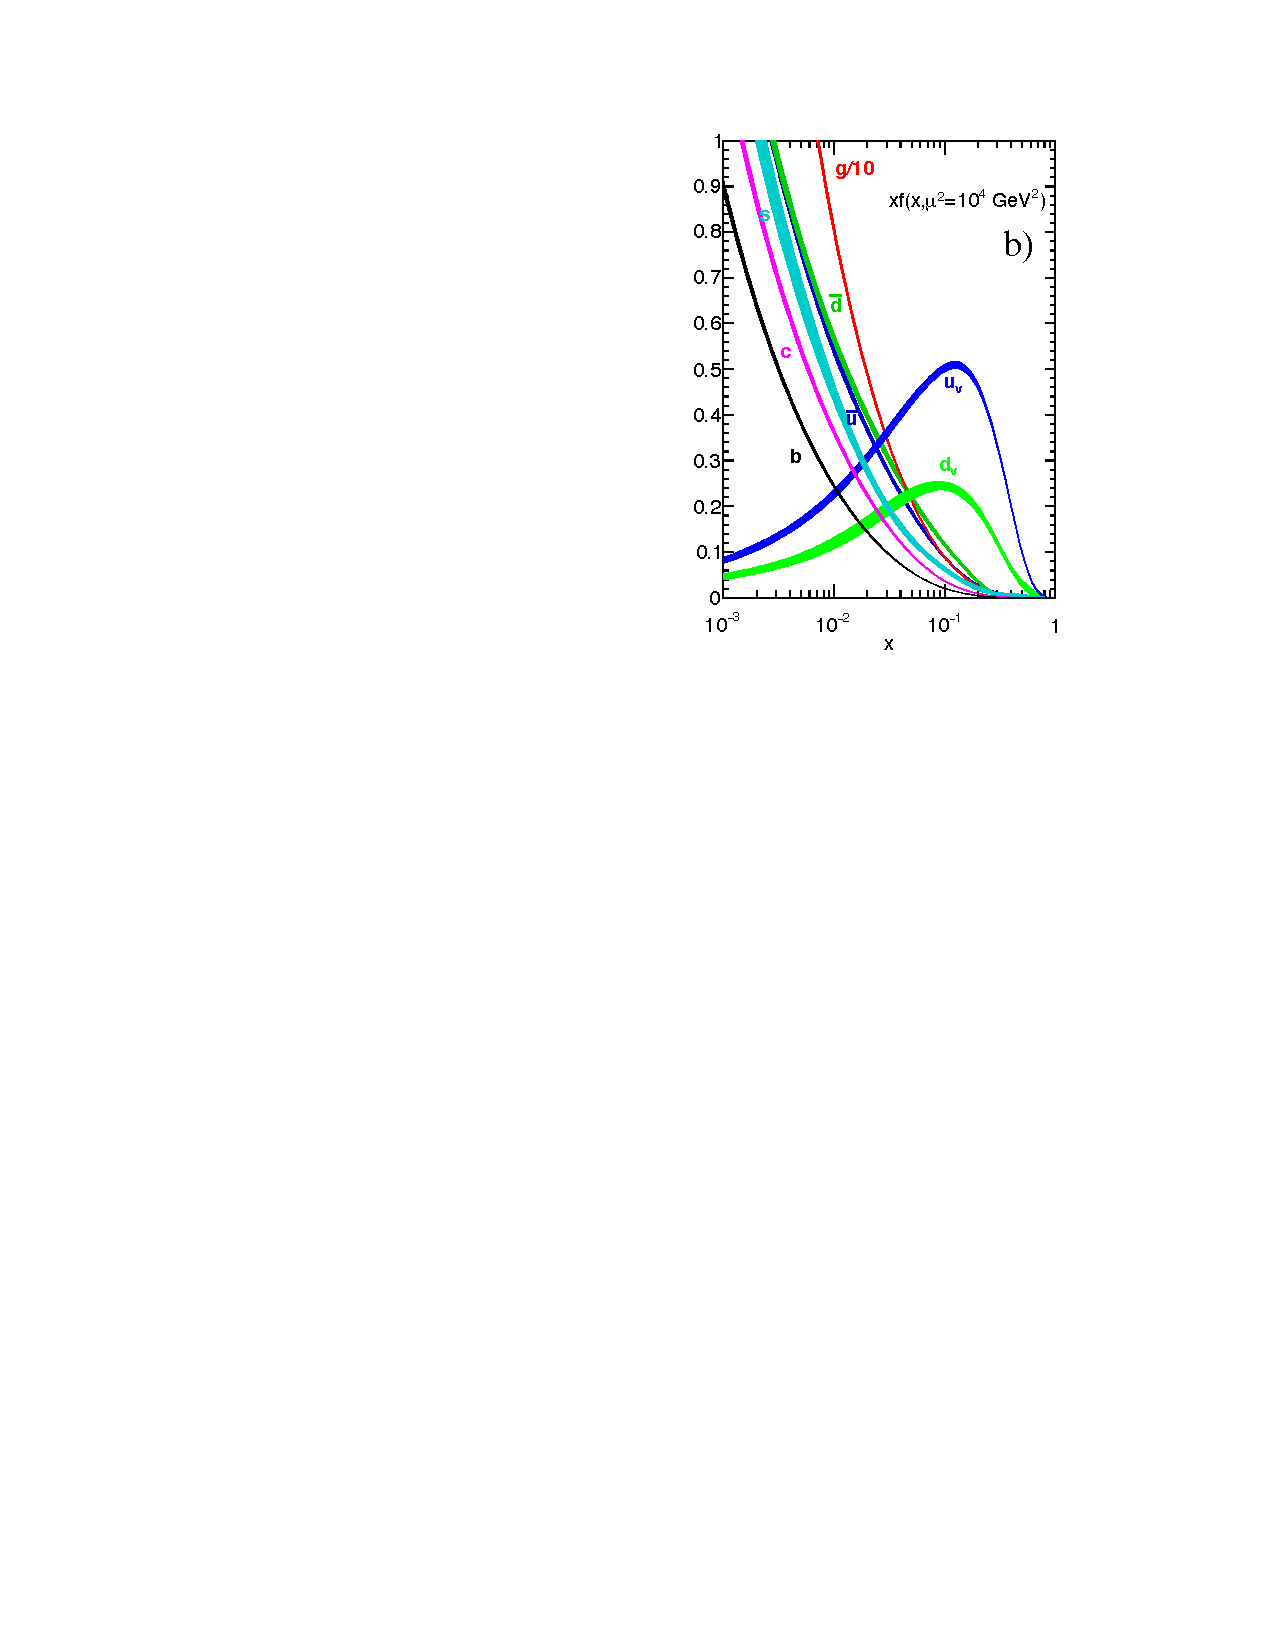
\includegraphics[width=\textwidth]{figures/production/pdf_sets_high_qsquared}};
  \begin{scope}[x={(image.south east)}, y={(image.north west)}]
    % Grid to help find coordinates on the image
    % \draw[step=0.02, gray, very thin] (0, 0) grid (1, 1);
    % Box to cover 'b)' label
    \path[fill=white] (0.82, 0.74) rectangle (0.94, 0.82);
  \end{scope}
\end{tikzpicture}

    \caption{High \pdfqsquared}
    \label{fig:prod:theory:pdf_sets:high_qsquared}
  \end{subfigure}
  \caption{%
    Sets of proton \aclp{QCDPDF} for low \pdfqsquared\ 
    (\subref*{fig:prod:theory:pdf_sets:low_qsquared}) and high \pdfqsquared\ 
    (\subref*{fig:prod:theory:pdf_sets:high_qsquared}), illustrating both 
    \bjorkenx\ and \pdfqsquared\ dependence~\cite{PDG2014}.
    Each band represents the \ac{QCDPDF} for a specific parton, as a function 
    of \bjorkenx, shown on the $x$-axis.
    The $\Pup_{\text{v}}$ and $\Pdown_{\text{v}}$ bands show the contributions 
    from the valance quarks, the \Pgluon band shows the gluon contribution, and 
    the other bands show the contribution from flavour-specific sea quarks.
  }
  \label{fig:prod:theory:pdf_sets}
\end{figure}

\subsection{Experimental input}
\label{chap:prod:theory:pdfs:inputs}

Today, inputs from both \ac{DIS} and hadron-hadron collider experiments serve 
to constrain proton \acp{QCDPDF} over a wide range of \bjorkenx\ and 
\pdfqsquared\ values.
The most recent and most powerful \ac{DIS} measurements have been made by the 
\hone\ and \zeus\ collaborations at the \hera\ $\Pe\Pproton$ 
collider~\cite{Abramowicz:1900rp}.
However, these measurements are largely constrained to measure values of 
\bjorkenx\ above \num{e-4}, leading to large uncertainties at low \bjorkenx.
This low-\bjorkenx\ region is particularly interesting to study not only 
because the current \ac{QCDPDF} uncertainties there are large, but also because 
it is where both the gluon and the sea quark contributions to the total 
\ac{QCDPDF} are large, as shown in \cref{fig:prod:theory:pdf_sets}, and so 
low-\bjorkenx\ measurements probe phenomenologically different processes.

In a hard \decay{2}{2} process, such as $\Pgluon\Pgluon$ fusion or \qqbar\ 
annihilation to a heavy quark pair, the extent in \bjorkenx\ that can be probe 
with heavy flavour hadron production measurements is given by
\begin{equation}
  {\bjorkenx}_{\text{min}} = e^{\pm\rapidity}\frac{%
    \sqrt{\pT^{2} + m_{\Pquark}^{2}}
  }{%
    \sqrts
  },
  \label{fig:prod:theory:hf_bjorkenx}
\end{equation}
where \rapidity\ and \pT\ parameterise the hadron kinematics, and $m_{q}$ is 
the mass of the heavy quark in the hadron under study~\cite{Zenaiev:2015rfa}.
There is then a wide range of \bjorkenx\ values that can be probed at proton 
colliders, with the highest sensitivity to low \bjorkenx\ provided by charm 
production measurements.\footnotemark\
At the \ac{LHC}, the dominant production mechanism is gluon-gluon fusion, as 
depicted in \cref{fig:intro:lhcb:hf_production:gg_fusion}, and so measurements 
at the \ac{LHC} are able to provide particularly strong constraints on the 
gluon densities.
Charm cross-sections have been measured in the $|\rapidity| < 0.5$ region for 
$\pT > \SI{1}{\GeVc}$ at \sqrtseq{2.76}\ and \sqrtseq{7}\ by the \alice\ 
collaboration~\cite{Abelev:2012sx,ALICE:2012ik,ALICE:2011aa},
and for pseudorapidity $|\Eta| < 2.1$ in the \pT\ region $3.5 < \pT < 
\SI{100}{\GeVc}$ at \sqrtseq{7} by the \atlas\ 
collaboration~\cite{Aad:2015zix}.

\footnotetext{%
  The charm quark mass is four times less than that of the bottom quark.
}

Measurements of charm production at \sqrtseq{7}\ were made by the \lhcb\ 
collaboration~\cite{LHCb-PAPER-2012-041}.
By \cref{fig:prod:theory:hf_bjorkenx}, measurements of charm hadron production 
for \pT\ values of the order of \SI{1}{\GeVc} at the lowest rapidities 
accessible to \lhcb\ can probe \bjorkenx\ values down to the order of \SI{e-6}, 
with lower values possible for measurements at a higher \sqrts, as shown in 
\cref{fig:prod:theory:prosa_x_regions}.
These measurements, along with similar measurements of beauty hadron production 
at \lhcb~\cite{LHCb-PAPER-2013-004} and the aforementioned \hone\ and \zeus\ 
measurements, have been used by the \prosa\ 
collaboration~\cite{Zenaiev:2015rfa} to constrain the proton \aclp{QCDPDF}, 
where they see a significant reduction on the gluon \ac{QCDPDF} uncertainty 
when including the \lhcb\ data, with respect to using the \hera\ data only, as 
shown in \cref{fig:prod:theory:prosa_gluon_pdf_fit}.
It is expected that additional measurements, at \sqrtseq{13}, can be used to 
further reduce the gluon \ac{QCDPDF} uncertainties~\cite{Gauld:2015yia}.

% \begin{figure}
%   \centering
%   \begin{tikzpicture}
  \begin{feynman}[scale=1.25,transform shape]
    \vertex (a);
    \vertex [right=of a] (b);

    \vertex [above left=of a] (i1) {\(\Pgluon\)};
    \vertex [below left=of a] (i2) {\(\Pgluon\)};

    \vertex [above right=of b] (f1) {\(\Pquark\)};
    \vertex [below right=of b] (f2) {\(\APquark\)};
    % Vertex in between b and f2, for the radiative gluon
    \vertex (bf1) at ($(b)!0.5!(f2)$);
    \vertex [right=of b] (f3);

    \diagram* [large] {
      (a) -- [gluon, edge label=\(\Pgluon\)] (b),
      (i1) -- [gluon] (a),
      (i2) -- [gluon] (a),
      (b) -- [fermion] (f1),
      (f2) -- [fermion] (b),
      (bf1) -- [gluon, edge label=\(\Pgluon\)] (f3),
    };
  \end{feynman}
\end{tikzpicture}

%   \caption{%
%     Feynman diagram of \qqbar\ pair production via \qqbar\ annihilation.
%   }
%   \label{fig:prod:theory:qqbar_annihilation}
% \end{figure}

\begin{figure}
  \centering
  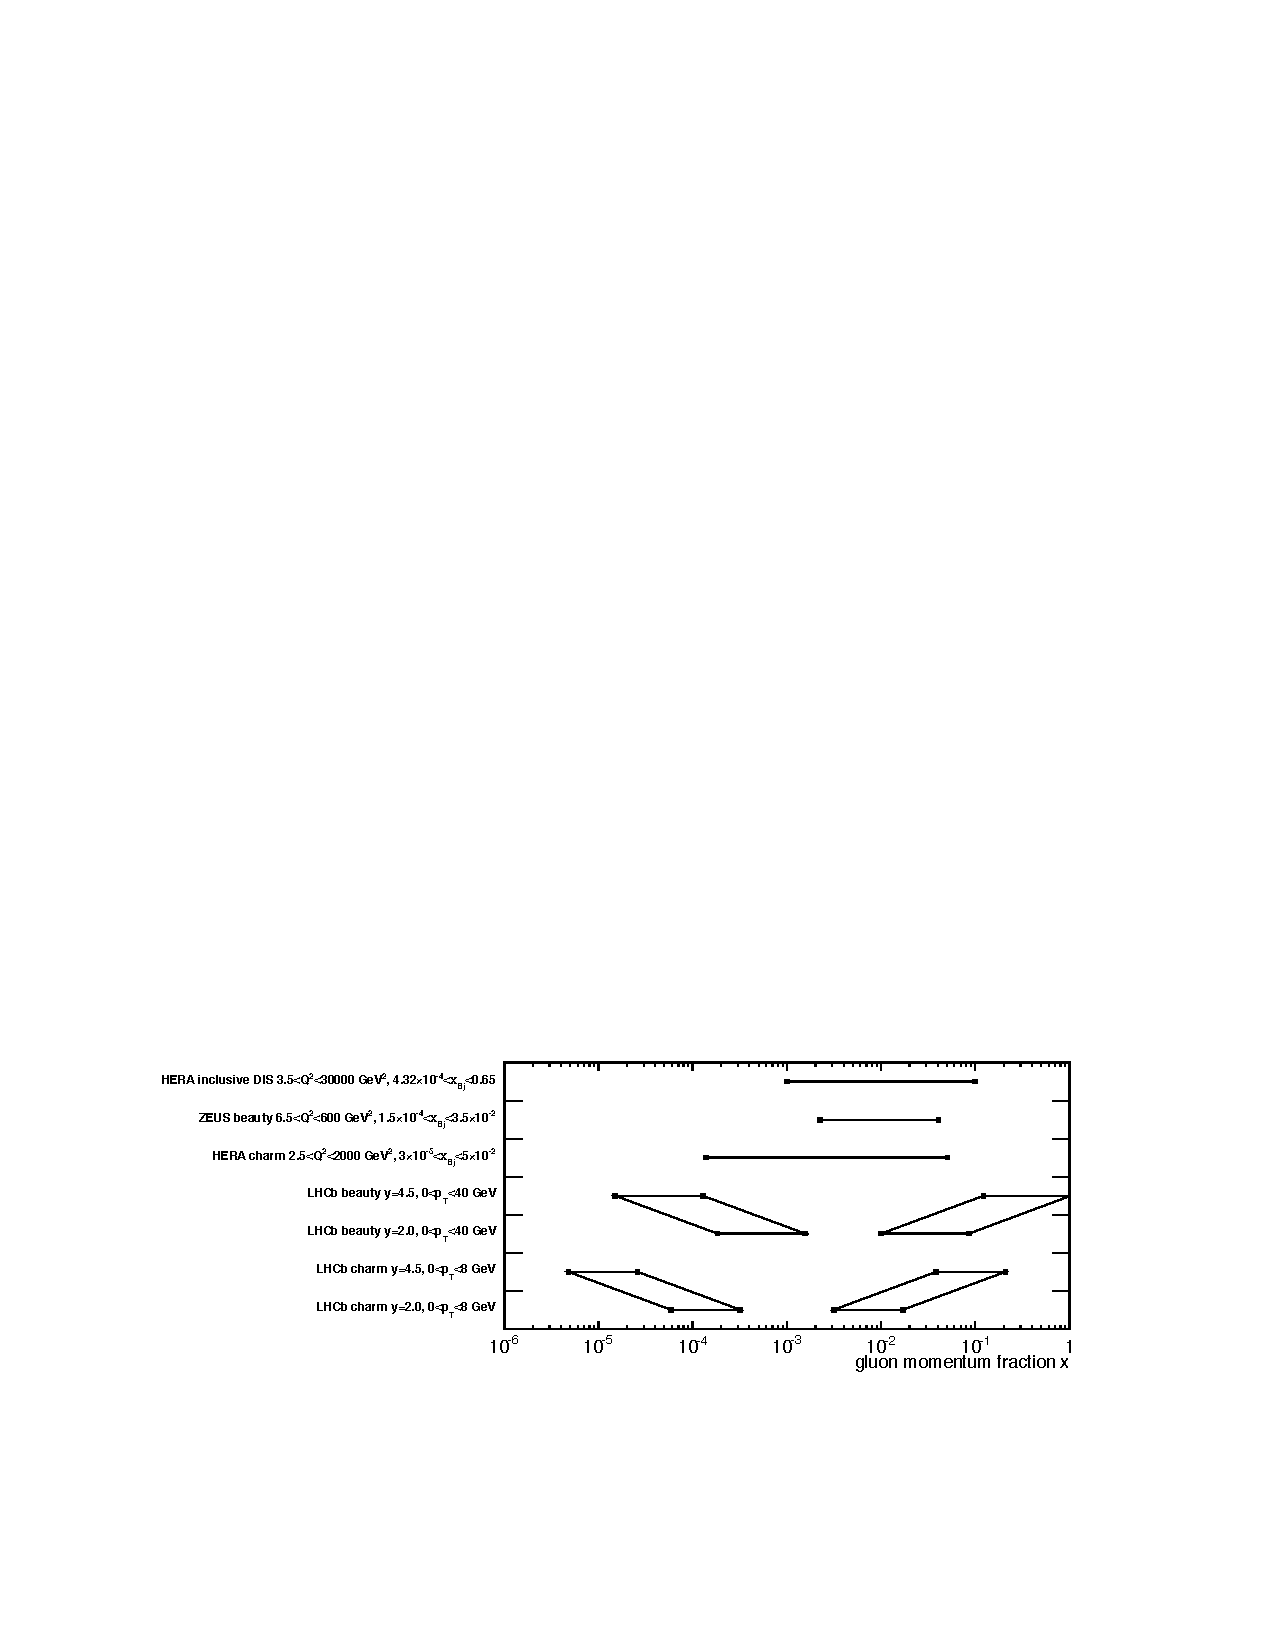
\includegraphics[width=\textwidth]{production/prosa_x_regions}
  \caption{%
    Regions of proton momentum fraction \bjorkenx, on the $x$-axis, probed by 
    different experiments, indicated on the $y$-axis~\cite{Zenaiev:2015rfa}.
  }
  \label{fig:prod:theory:prosa_x_regions}
\end{figure}

\begin{figure}
  \centering
  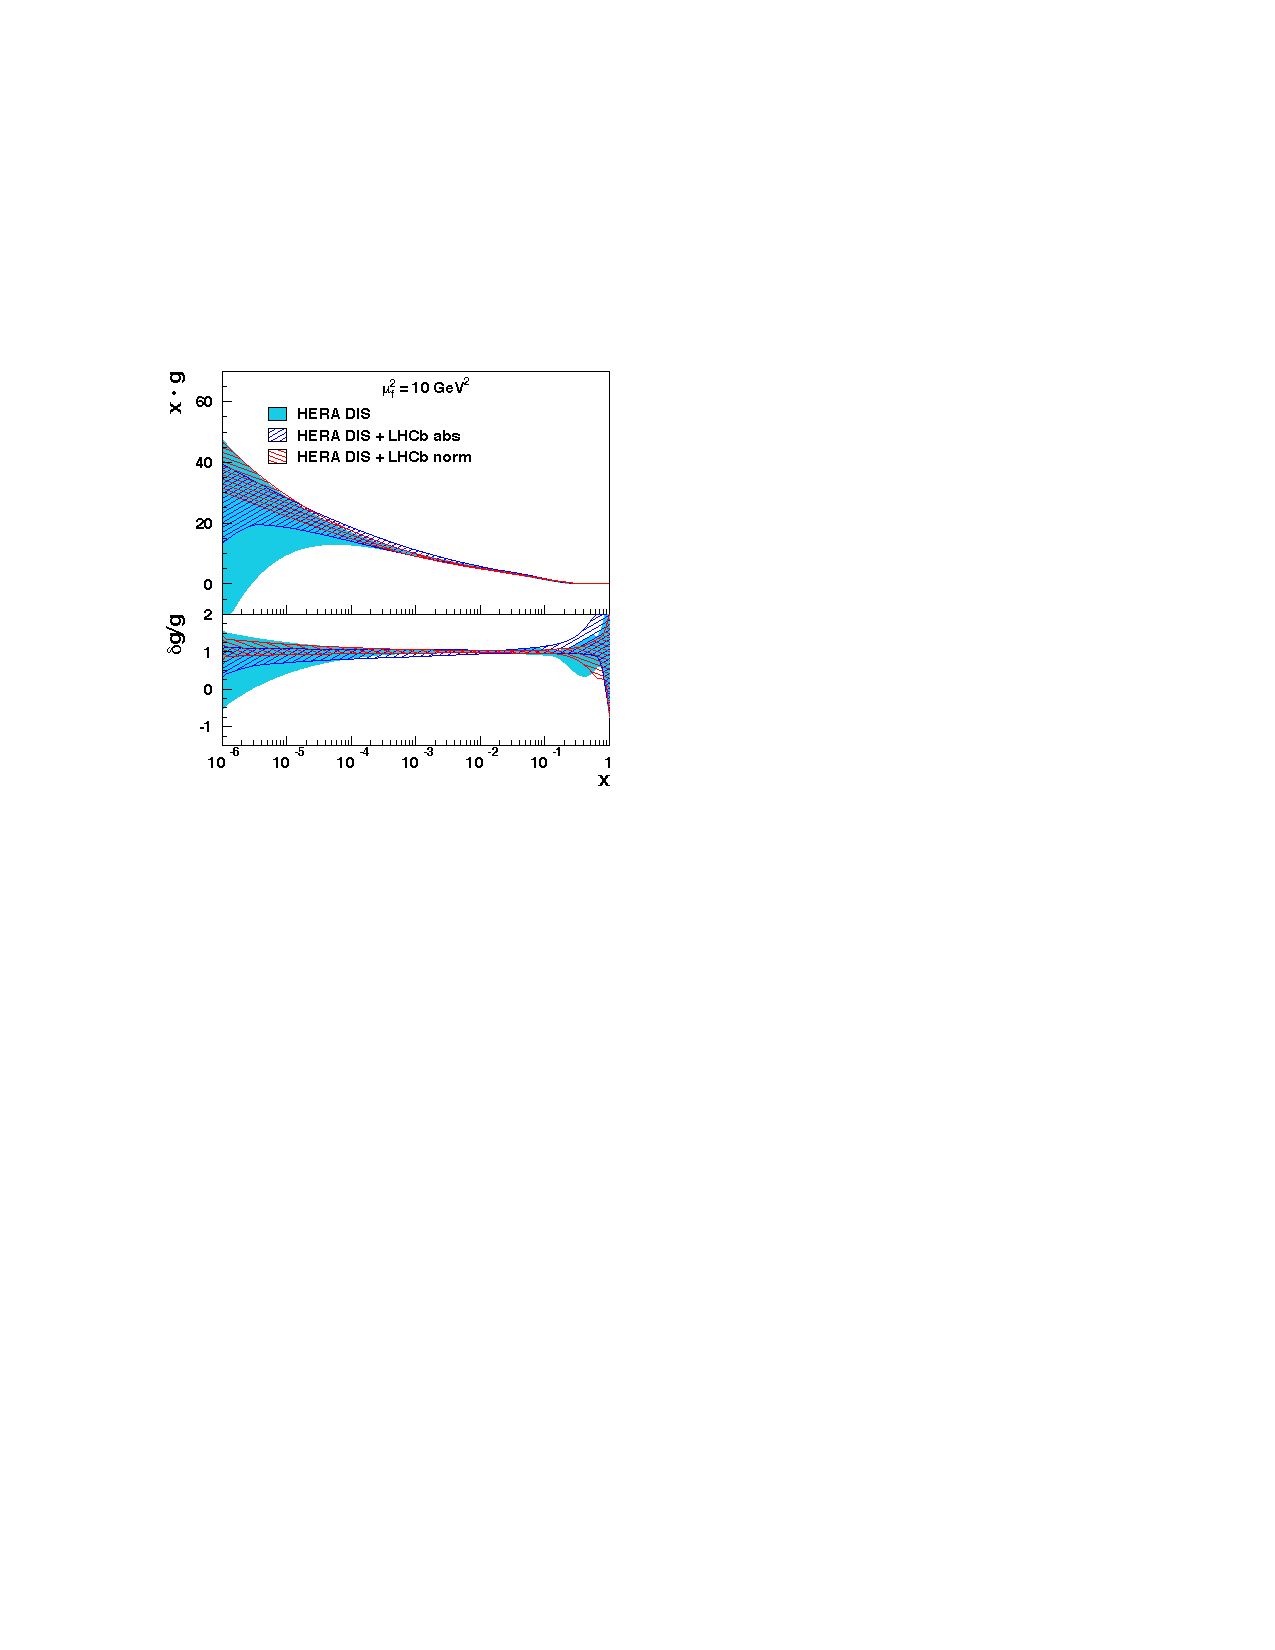
\includegraphics[width=\textwidth]{production/prosa_gluon_pdf_fit}
  \caption{%
    Gluon \acp{QCDPDF} after fitting to experimental 
    data~\cite{Zenaiev:2015rfa}.
    The $x$-axis shows the proton momentum fraction \bjorkenx, the $y$-axis on 
    the top plot shows the gluon \ac{QCDPDF} density, and the $y$-axis on the 
    bottom bottom shows the relative uncertainty on the model.
    The solid band shows the fit when only using the \hera\ measurements as 
    inputs, whilst the hatced bands show the fit when using both the \hera\ and 
    \sqrtseq{7}\ \lhcb\ measurements.
  }
  \label{fig:prod:theory:prosa_gluon_pdf_fit}
\end{figure}

\section{Atmospheric neutrino fluxes}
\label{chap:prod:theory:neutrinos}

The constraints imposed on the proton \acp{QCDPDF} are also useful in 
atmospheric neutrino experiments.
The \icecube\ collaboration aims to measure highly energetic neutrinos of 
astrophysical origin with energies up to the \si{\peta\eV} scale, using the 
IceCube Neutrino Observatory~\cite{Achterberg:2006md}.
This is done to shed light on the mystery of ultra-high-energy cosmic rays 
(protons) whose source is unknown but should also produce similarly energetic
neutrinos.
The so-called conventional neutrino flux constitutes one of the backgrounds for 
astrophysical neutrino experiments.
This is made by cosmic rays interacting in the atmosphere and producing pions 
and kaons, which then decay to final states containing neutrinos.
However, for the high energies the \icecube\ detector is sensitive to, 
beginning at around \SI{100}{\GeV}, this background is suppressed.
The long lifetime of the mesons increases the probability they will interact 
with the atmosphere in flight, losing energy through hadronic interactions, 
hence reducing the energy spectrum of the resulting neutrinos.
However, an additional background comes from the production of charm hadrons in 
the atmosphere, which, with their comparatively short lifetimes, lose very 
little energy in flight, and so the neutrino spectrum from charm decays is very 
similar to the cosmic ray energy spectrum.
The neutrinos produced in the charm decays can interact with the detector in a 
similar manner to the signal and exhibit a similar energy spectrum.
It is then of key importance that the amount of expected background from these 
decays is known, else neutrinos from charm decays may be misinterpreted as 
neutrinos from astrophysical sources.
This contamination can be estimated by predicting the proton-proton 
cross-sections (between the cosmic ray and the nuclei in the atmosphere).

Colliding equal-energy proton-proton beams at a centre-of-mass energy of 
\SI{13}{\TeV} is equivalent to directing a proton beam of energy 
\SI{100}{\peta\eV} into a fixed target, as $\sqrts \approx 
\sqrt{2E_{\Pproton}m_{\Pproton}}$, where $E_{\Pproton}$ is the energy of the 
proton beam and $m_{\Pproton}$ is the proton mass.
Hence, measuring charm cross-sections at \sqrtseq{13}\ at the \ac{LHC} can 
provide constraints on the expected rate of charm production in the atmosphere 
produced by extremely high-energy cosmic rays.
Indeed, the measurements made by \lhcb\ at \sqrtseq{7}\ have already been used 
to that effect, and additional measurements at \SI{13}{\TeV} can help 
further~\cite{Gauld:2015yia,Bhattacharya:2015jpa}.

\section{Cross-section comparisons with theory}
\label{chap:prod:theory:comparisons}

A useful check of \acp{QCDPDF} constrained with past experimental data is to 
compute cross-section predictions using them, for comparison with new 
experimental results.
This was done in the previous \lhcb\ open charm cross-section analysis, shown 
in \cref{fig:prod:theory:comparisons:7tev}, where at low \pT\ the data 
generally lie above the theory prediction.
Additional measurements can help in the understanding of these discrepancies.

For the analysis presented in this \namecref{chap:prod}, a measurement of charm 
production at \sqrtseq{13}, three theory groups have provided predictions for 
the double differential cross-sections.
Each set of predictions is computed at next-to-leading order in the strong 
coupling constant \alphas\ (that is, up to the first power of $\alphas$), and 
includes uncertainties from: the factorisation scale dependence, which is the 
scale \pdfqsquared\ at which the perturbative expansion was made; and the 
renormalisation scale, which is the scale at which the expansion is 
renormalised to remove ultraviolet divergences.
These affect both the evaluation of the partonic cross-sections and the 
evolution of the \ac{QCDPDF} sets with the \ac{DGLAP} equations.

The \nnpdfl\ predictions~\cite{Gauld:2015yia} use a \ac{QCDPDF} set that 
includes the constraints from the \sqrtseq{7}\ \lhcb\ 
measurement~\cite{LHCb-PAPER-2012-041}, and are provided for all \pTy\ bins for 
\PDz and \PDp mesons.
The \ac{GMVFNS} predictions~\cite{Kniehl:2012ti} are provided for $\pT > 
\SI{3}{\GeVc}$ for all mesons under study, and use the CT10 \ac{QCDPDF} set.
These predictions include a factor to account for the \cToHc\ transition 
probability, obtained by convolving the \decay{\ccbar}{\PHc} cross-sections 
with the appropriate fragmentation functions.
Finally, \ac{FONLL} predicitions~\cite{Cacciari:2015fta} using the \nnpdf\ 
\ac{QCDPDF} sets are provided for for the full \pTy\ phase space for \PDz, 
\PDp, and \PDstarp mesons.
The \fonll\ predictions assume a unit \cToHc\ transition probability, and so 
are multiplied by the fragmentation fractions in 
\cref{tab:prod:introduction:fragmentation_fractions} for comparison with the 
measurements.
The comparison of these predictions with the data will be given in 
\cref{chap:prod:results}.

\begin{figure}
  \centering
  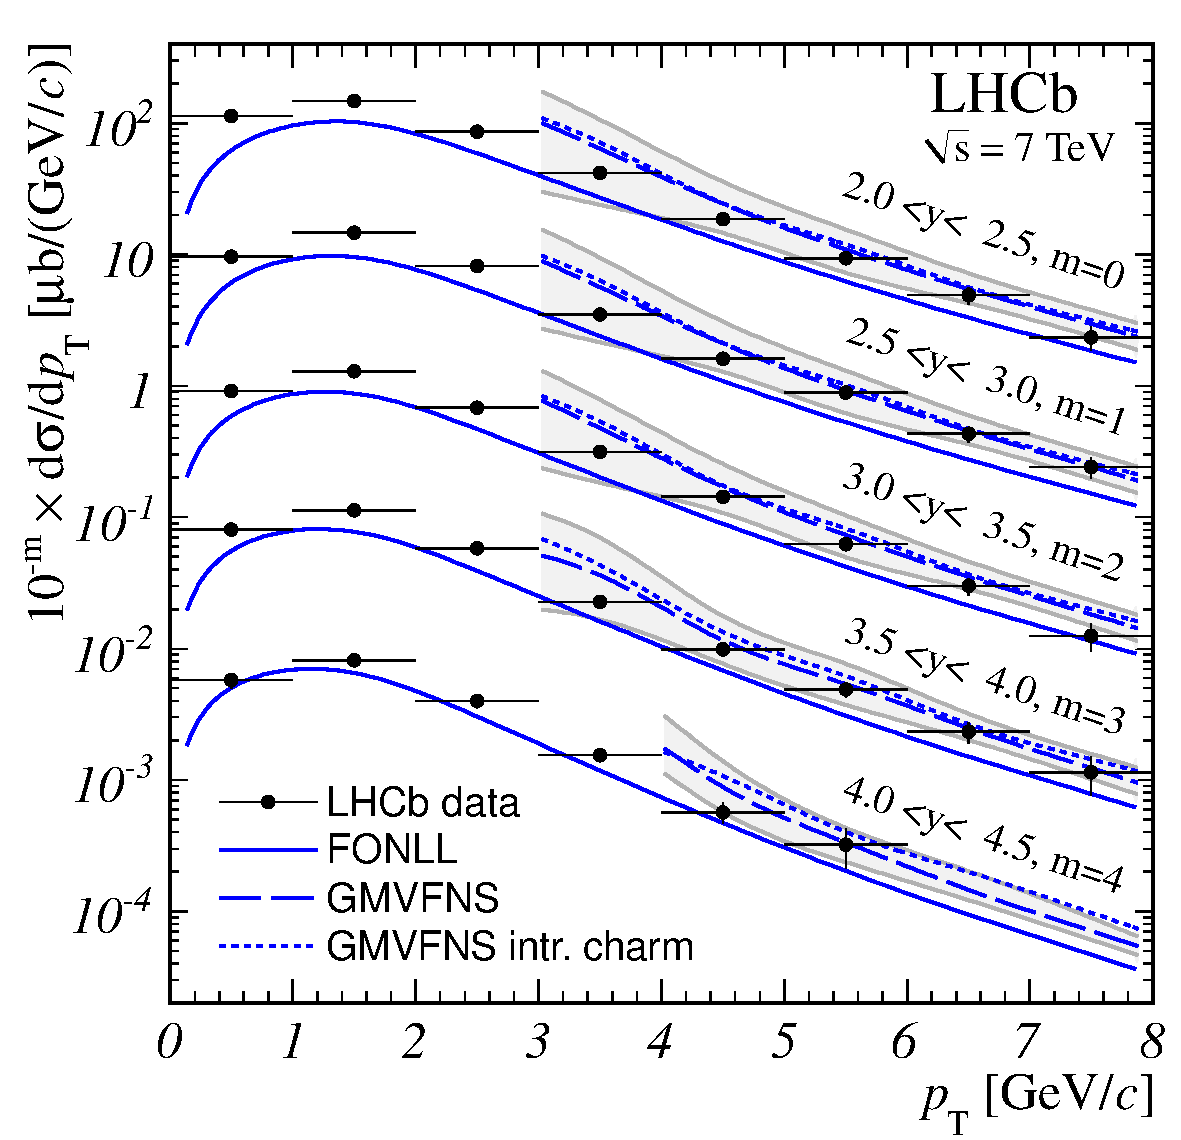
\includegraphics[width=\textwidth]{production/lhcb_dz_xsec_7tev}
  \caption{%
    Prompt \PDzero production rates, measured using the \lhcb\ detector with 
    proton-proton data taken at \sqrtseq{7}~\cite{LHCb-PAPER-2012-041}, in 
    \pTy\ bins.
    The $x$-axis shows the \pT\ of the \PDzero, and the measurements are offset 
    by a multiplicative factor based on the rapidity bin.
  }
  \label{fig:prod:theory:comparisons:7tev}
\end{figure}


\chapter{Datasets and running conditions}
\label{chap:prod:data}

% Luminosity determination
% LHC conditions
% Trigger set up

\lipsum[1-2]


\chapter{Event and candidate selection}
\label{chap:prod:sel}

The decay modes chosen for this analysis,
\DzToKpi, \DpToKpipi, \DspTophipi\ with \phiToKK, and \DstToDzpi\ with 
\DzToKpi, including their charge conjugates, are the amongst the most probable 
fully charged, hadronic final states for each meson.
The advantage of choosing such final states is that it allows the invariant 
mass of the charm hadrons to be computed unambiguously, so that a yield 
determination can be performed by modelling the peaking signal structure in the 
mass distribution via fits.
These fits shall be discussed in detail in \cref{chap:prod:fitting}, but it is 
worth noting at this point that such fits are simpler if the data is `clean', 
that is if the fraction of charm meson signal in the data is high.
It is then advantageous to optimise the selection of the data to reduce 
backgrounds, whilst retaining as much signal as possible to maximise the 
statistical precision of the measurement.

The selection of fully charged, hadronic decay modes of charm mesons has 
already been performed by many other analysis at \lhcb,\footnotemark and their 
selections share several common features.
The first of these is a requirement on the minimum charm candidate \pT, as 
there are many soft particles produced directly in the proton-proton collision, 
and such a requirement removes many of them.
The second is to ask that the charm candidate vertex is significantly displaced 
from the proton-proton collision vertex, or \ac{PV}, exploiting the long flight 
distances of charm hadrons in the laboratory frame.
Finally, it is required that the \ipchisq\ of the charm meson, a measure of the 
\acf{IP} relative to the uncertainty on the \ac{IP}, does not exceed a certain 
value.
This suppresses the background of charm candidates whose three-momentum does 
not point back to the \ac{PV}, which the momentum of random combinations of 
tracks will not, on average.
Each of these three features are powerful discriminators between signal and 
background.

\footnotetext{%
  Representative examples include selections of 
  \decay{\PDzero}{\PKmp\Ppipm}~\cite{Aaij:2012nva}, 
  \decay{\PDp}{\PKminus\PKplus\Ppiplus}~\cite{Aaij:2011cw}, and 
  \DspTophipi~\cite{Aaij:2012cy} decays.
}

For this measurement of prompt charm production it is preferable not to make 
\pT\ requirements on the charm candidate as they would restrict the \pT\ range 
available for differential measurements.
Nor is it desirable to make \ipchisq\ cuts, as the \ipchisq\ distribution is 
used for prompt-secondary discrimination, and having access to only part of the 
distribution can hinder accurate modelling.
The selection used is then informed by previous \lhcb\ studies of fully 
charged, hadronic charm decays, but with modifications to improve the utility 
for the measurement in hand.
The selection variables that are useful for discriminating between signal and 
background, in addition to those discussed, are given and described below.
The `parent' is the charm hadron \PHc, and the `children' are the charged 
hadrons in the final state.

\begin{description}
  \item[Child track \chisq\ per degree of freedom] \hfill \\
    The \chisq\ per degree of freedom of the child track returned by the track 
    fit.
    This variable discriminates between real and fake~(ghost) tracks.
  \item[Child transverse momentum] \hfill \\
    Momentum transverse to the $z$-axis.
    Children of charm hadrons will have a higher \pT\ on average than prompt 
    stable particles produced directly from the \pp\ collision.
  \item[Child momentum] \hfill \\
    Three-momentum magnitude \ptot.
    Must be within the range of acceptable particle identification performance 
    and fall within the kinematic spectrum of the \ac{PID} calibration samples, 
    discussed in \cref{chap:prod:effs:pid}.
  \item[Child pseudorapidity] \hfill \\
    Pseudorapidity \Eta, defined in \cref{eqn:intro:lhcb:pseudorapidity}.
    Must be within the range of acceptable particle identification performance 
    and fall within the kinematic spectrum of the \ac{PID} calibration samples.
  \item[Child \ipchisq] \hfill \\
    Impact parameter with respect to the \ac{PV}, as shown 
    in~\cref{fig:intro:lhcb:vertexing}.
    Prompt stable particles produced directly in the \pp\ collision will have a 
    low impact parameter, whereas particles produced in long-lived charm decays 
    will not have trajectories pointing back to the \ac{PV} on average.\\
    The `\chisq' is computed as $\Delta^{\text{T}}\Sigma^{-1}\Delta$, where 
    $\Delta$ is the difference in the position vectors of the track and the 
    vertex, and $\Sigma$ is the sum of the covariance matrices of the track and 
    vertex fits.
    This quantity is approximately equal to the ratio of the \ac{IP} and the 
    uncertainty on that \ac{IP} measurement.
  \item[Child \ac{PID}] \hfill \\
    Particle identification information as the combined response of the 
    calorimeters, muon stations, and \rich\ detectors, as described in 
    \cref{chap:intro:lhcb:detector:pid}.
  \item[Pairwise child \ac{DOCA}] \hfill \\
    For a set of tracks physically originating from a common vertex, the 
    largest distance between any two tracks, the \ac{DOCA}, should be small.
  \item[Parent reconstructed mass] \hfill \\
    Invariant mass, either computed before the vertex fit as the sum of the 
    child four-momenta, or after as the mass of the fitted vertex.
    In a signal sample, a peaking structure will be seen around the nominal 
    charm hadron invariant mass.
    To be able to model the combinatorial background, the window around the 
    nominal mass should be many times wider than the resolution on this peak.
  \item[Parent vertex quality] \hfill \\
    Quality of the vertex fit.
    A larger \chisq\ value means a lower probability that the input tracks 
    originated from the same spatial point, which would be true if the tracks 
    were the product of a particle decay.
  \item[Parent vertex displacement] \hfill \\
    Displacement of the secondary (decay) vertex from the \ac{PV}, assumed to 
    be the \ac{PV}, as either the reconstructed lifetime $c\lifetime$ or the 
    vertex displacement \chisq.
    The `\chisq' is computed as $\Delta^{\text{T}}\Sigma^{-1}\Delta$, where 
    $\Delta$ is the difference in the spatial positions of the two vertices, and 
    $\Sigma$ is the sum of the covariance matrices of the two vertex fits.
  \item[Parent \ac{DIRA}] \hfill \\
    If the child tracks are from a true decay, all of the child tracks have 
    been reconstructed, and the decay vertex position is correctly 
    reconstructed, then the momentum vector of the parent should point in the 
    same direction as the displacement vector between the \ac{PV} and the decay 
    vertex.
    The angle between the momentum and displacement vectors, the \ac{DIRA}, 
    should be small for a correctly reconstructed signal decay.
\end{description}

The exact numerical requirements made on these quantities were not tuned to 
optimise any specific figure of merit.
Instead, the values were chosen based on those used in previous charm analysis, 
generally being loosened to account for the higher rate available to charm 
triggers during the early measurements period, and the desire to have as high 
an efficiency as possible in the low \pT\ regions of the measurement.

As this analysis uses the Turbo stream, the only selection is `online', in that 
it is only performed on quantities computed in the trigger.
Still, the values computed are available `offline', once the data has been made 
available to analysts.
The selection is then split in two: the `online' part, which is the selection 
defined in the trigger and cannot be tuned once the data has been taken, and 
the `offline' selection, which is any selection made after this.
The use of the Turbo stream permits only one pass of the full event 
reconstruction, that done `online' in the trigger.
The following \namecref{chap:prod:sel:online} shall detail the online selection 
and reconstruction, and will be followed by a description of the offline 
selection in \cref{chap:prod:sel:offline}.

\section{Online selection and reconstruction}
\label{chap:prod:sel:online}

The different purpose and hierarchy of the different stages of the \lhcb\ 
trigger are described in \cref{chap:intro:lhcb:detector:trigger}.
For this analysis, at \lzero\ bunch-bunch crossings are accepted randomly by 
the \nobias\ trigger, so called because it should not bias any distributions of 
interest.
The rate at which the \nobias\ trigger accepts events is programmed into the 
hardware controller manually, with the exact rate depending on the number of 
colliding bunches at \lhcb.
The rates were tuned throughout the early measurements period so as to keep the 
detector `dead time' to a minimum.\footnotemark\
The \lzero\ rate is given for each fill in 
\cref{tab:prod:sel:online:l0_nobias_rateeff}.

\footnotetext{%
  The detector dead time is the period during which triggers by the \lzero\ are 
  `lost' due to the read-out buffer being full.
  The buffer is able to hold 16 events, each of which takes 40 \ac{LHC} clock 
  cycles, of \SI{25}{\nano\second} each, to be sent to the \hlt.
  Dead time can then occur if several triggers occur too close to one 
  another~\cite{Schmelling:1998qta}.
}

In \hltone, the following sequence is performed for events passing \lzero:
\begin{enumerate}
  \item The full offline charged particle (track) reconstruction is run for 
    hits inside the \velo\ sub-detector;
  \item The full offline \ac{PV} reconstruction is run, using as input only the 
    \velo\ tracks reconstructed in the previous step; and
  \item The reconstruction of `long' tracks, by first extrapolating \velo\ 
    tracks into the \ttracker\ and then, if at least two matching hits are 
    found in the \ttracker, extrapolating through the magnetic field.
    To decrease the time taken to assess all combinatorial combinations of 
    \velo+\ttracker\ tracks with hits in the \itracker\ and \otracker, only 
    hits within a search window assuming a \pT\ of at least \SI{800}{\MeVc} are 
    considered.
\end{enumerate}
Requiring all child tracks from a vertex to have $\pT > \SI{800}{\MeVc}$ would 
be inefficient for low \pT\ charm hadrons, and so the full decay is not 
reconstructed in \hltone.
Instead, the presence of a single, good quality track is required, which is 
consistent with having originated from a heavy flavour decay by having a large 
\ipchisq.
The full set of selection requirements is given in 
\cref{tab:prod:sel:online:hlt1_selection}.

\hlttwo\ performs the full, offline-quality event reconstruction on events 
passing \hltone.
One \hlttwo\ selection, or `\hlttwo\ line', is defined per charm decay 
topology, corresponding to: one line for \DzToKpi; one line for the charged 
three-body decays, specifically \DpToKpipi\ and \DspToKKpi; and one line for 
\DstToDzpi.
In the \PDzero, \PDplus, and \PDsplus lines, candidates are made by combining 
long tracks whose particle hypotheses are consistent with the final state under 
consideration.
In the \PDstarp\ line, \PDzero\ candidates passing the \PDzero\ \hlttwo\ line 
are combined with pion candidates, referred to here as `soft pions', 
\Ppiplussoft, due to their soft momentum distribution.
There are three stages to the particle combination: when cuts are applied to 
the input tracks; when cuts are applied to the four-vector sum of these tracks; 
and when cuts are applied to the fitted vertex.
To save computing resources, the combination does not proceed past a failing 
step, and combinations where the vertex fit fails to converge are discarded, 
although the likelihood of a failing vertex fit is suppressed by making 
\ac{DOCA} requirements beforehand.
An event is saved for offline analysis if at least one \hlttwo\ line `fired', 
that is if a charm candidate is made that passes all cuts.
The \DzToKpi, \DTohhh, and \DstToDzpi\ requirements are given in 
\cref{tab:prod:sel:online:hlt2_dztokpi_selection,tab:prod:sel:online:hlt2_dtohhh_selection,tab:prod:sel:online:hlt2_dsttodzpi_selection}.
Distributions of the charm candidate invariant mass after the full trigger 
selection are given in 
\cref{fig:prod:sel:D0ToKpi:online,fig:prod:sel:DpToKpipi:online,fig:prod:sel:DsToKKpi:online,fig:prod:sel:DstToD0pi_D0ToKpi:online}.

\begin{table}
  \caption{%
    List of fills used in analysis, along with the integrated luminosity 
    \intlumi, the \lzero\ \nobias\ rate, and the corresponding effective 
    \lzero\ efficiency (``eff.'') for each fill.
  }
  \label{tab:prod:sel:online:l0_nobias_rateeff}
  \centering
  \begin{tabular}{lS[table-figures-uncertainty=1]cS[table-format=2.2]}
  \toprule
  Fill number & {\intlumi (\si{\per\nb})} & \lzero\ \nobias\ rate (\si{\kilo\hertz}) & {\lzero\ \nobias\ eff. (\si{\percent})} \\
  \midrule
  3976        & 628 \pm 24                & 250                                      & 20.58                                   \\
  3981        & 1101 \pm 43               & 300                                      & 10.84                                   \\
  3988        & 931 \pm 36                & 300                                      & 10.84                                   \\
  3992        & 1310 \pm 51               & 350                                      & 7.84                                    \\
  3996        & 999 \pm 39                & 350                                      & 7.84                                    \\
  \bottomrule
\end{tabular}

\end{table}

\begin{table}
  \caption{%
    Requirements made on the track that fires the \hltone\ trigger line.
  }
  \label{tab:prod:sel:online:hlt1_selection}
  \centering
  \begin{tabular}{lcc}
  \toprule
  Particle                   & Variable     & Cut value          \\
  \midrule
  \multirow{5}{*}{Any track} & \pT          & $> \SI{800}{\MeV}$ \\
                             & \ptot        & $> \SI{3}{\GeV}$   \\
                             & Track \chisq & $< 3$              \\
                             & \ipchisq     & $> 10$             \\
                             & \velo\ hits  & $> 9$              \\
  \bottomrule
\end{tabular}

\end{table}

\begin{table}
  \caption{%
    Requirements made in the \hlttwo\ \DzToKpi\ selection.
    The track \chisq\ criterion is applied in the reconstruction and listed 
    here for completeness.
  }
  \label{tab:prod:sel:online:hlt2_dztokpi_selection}
  \centering
  \begin{tabular}{lccc}
  \toprule
  Particle                        & Variable                   &
  Cut value                      \\
  \midrule
  \multirow{4}{*}{\Ppipm, \PKpm}  & \pT                        & $> \SI{250}{\MeV}$                      \\
                                  & \ptot                      & $\ptot > \SI{2}{\GeV}$                  \\
                                  & Track \chisq               & $< 3$                                   \\
                                  & \ipchisq                   & $> 16$                                  \\
  \midrule
  \Ppipm                          & \dllkpi                    & $< 5$                                   \\
  \midrule
  \PKpm                           & \dllkpi                    & $> 5$                                   \\
  \midrule
  \multirow{5}{*}{\PDzero}        & $m(\PKminus\Ppiplus)$      & $\SI{1784}{\MeV} < m < \SI{1944}{\MeV}$ \\
                                  & \PK to \Ppi DOCA           & $< \SI{0.1}{mm}$                        \\
                                  & Vertex fit \chisq          & $< 10$                                  \\
                                  & Direction angle            & $< \SI{17}{\milli\radian}$              \\
                                  & Vertex displacement \chisq & $> 49$                                  \\
  \bottomrule
\end{tabular}

\end{table}

\begin{table}
  \caption{%
    Requirements made in the \hlttwo\ \DTohhh\ selection.
    The \PDp and \PDsplus candidates are defined according to the three-body 
    mass window after the vertex fit.
    Cuts of the form $x > x_{1},\, x_{2},\, x_{3}$ require that all particles 
    satisfy $x > x_{1}$, at least two satisfy $x > x_{2}$, and at least one 
    satisfies $x > x_{3}$.
    The track \chisq\ criterion is applied in the reconstruction and listed 
    here for completeness.
  }
  \label{tab:prod:sel:online:hlt2_dtohhh_selection}
  \centering
  \begin{tabular}{lccc}
  \toprule
  Particle                          & Variable                   & Cut value                                           \\
  \midrule
  \multirow{4}{*}{\Ppipm, \PKpm}    & \pT                        & $> 200,\, 400,\, \SI{1000}{\MeV}$                   \\
                                    & \ptot                      & $\ptot > \SI{2}{\GeV}$                              \\
                                    & Track \chisq               & $< 3$                                               \\
                                    & \ipchisq                   & $> 4,\, 10,\, 50$                                   \\
  \midrule
  \Ppipm                            & \dllkpi                    & $< 5$                                               \\
  \midrule
  \PKpm                             & \dllkpi                    & $> 5$                                               \\
  \midrule
  \PDplus                           & $m(\Phm\Php\Php)$          & $\SI{1789}{\MeV} < m < \SI{1949}{\MeV}$             \\
  \midrule
  \PDsplus                          & $m(\Phm\Php\Php)$          & $\SI{1889}{\MeV} < m < \SI{2049}{\MeV}$             \\
  \midrule
  \multirow{3}{*}{\PDplus/\PDsplus} & Vertex fit \chisq          & $< 25$                                              \\
                                    & Direction angle            & $< \SI{35}{\milli\radian}$                          \\
                                    & Vertex displacement \chisq & $> 16$ \text{AND} $\tau > \SI{0.150}{\pico\second}$ \\
  \bottomrule
\end{tabular}

\end{table}

\begin{table}
  \caption{%
    Requirements made in the \hlttwo\ \DstToDzpi\ selection.
    The input \PDzero\ candidates are those passing the \PDzero selection 
    defined in \cref{tab:prod:sel:online:hlt2_dztokpi_selection}.
    The track \chisq\ criterion is applied in the reconstruction and listed 
    here for completeness.
  }
  \label{tab:prod:sel:online:hlt2_dsttodzpi_selection}
  \centering
  \begin{tabular}{lccc}
  \toprule
  Particle                  & Variable                 & Cut value                             \\
  \midrule
  \multirow{2}{*}{\Ppipm}   & \pT                      & $> \SI{100}{\MeV}$                    \\
                            & Track \chisq             & $< 3$                                 \\
  \midrule
  \multirow{2}{*}{\PDstarp} & $m(\PDstarp)-m(\PDzero)$ & $\SI{130}{\MeV} < m < \SI{160}{\MeV}$ \\
                            & Vertex fit \chisq        & $< 25$                                \\
  \bottomrule
\end{tabular}

\end{table}

\section{Offline selection}
\label{chap:prod:sel:offline}

To improve the purity of the samples, the pion \ac{PID} requirement is 
tightened to $\dllkpi < 3$.
Furthermore, kinematic requirements are made on all \PDzero, \PDplus, and 
\PDsplus children such that they are within the fiducial region of phase space 
available for \ac{PID} efficiency calibration, which will be described in 
\cref{chap:prod:effs:pid}, specifically $3 < \ptot < \SI{100}{\GeVc}$ and $2 < 
\Eta < 5$.
As the three-body samples contain a large fraction of combinatorial background 
even after these additional cuts, the vertex fit \chisq\ and the direction 
angle cuts are tightened to $\chisq < 6$ and $\ac{DIRA} < 
\SI{14}{\milli\radian}$.

To reduce the combinatorial further in the \DspToKKpi\ data, a requirement is 
made on the kaon pair as
\begin{equation}
  999.46 < m(\PKminus\PKplus) < \SI{1039.46}{\MeVcc}.
  \label{eqn:prod:sel:phi_cut}
\end{equation}
This corresponds to a $\pm\SI{20}{\MeVcc}$ window around the nominal mass of 
the $\phi(1020)$ meson~\cite{PDG2014}, which is referred to here as just 
`\Pphi'.
Around half of all \DspToKKpi\ decays proceed via the 
$\decay{\Pphi}{\PKminus\PKplus}$ channel~\cite{PDG2014}, and the narrow width 
of the \Pphi resonance makes this cut efficient at reducing the fraction of 
combinatorial background in the data, as well as reducing the fraction of $\Ppi 
\to \PK$ mis-identifications.
As the \DspToKKpi sample is then dominated by resonant \DspTophipi, the 
\PDsplus sample is referred as `\DspTophipi'.
The effective reduction of the total number of \PDsplus mesons produced due to 
the \Pphi requirement is treated as part of the branching fraction contribution 
in \cref{eqn:prod:introduction:differential_cross_section}, rather than as part 
of the selection efficiency.
The \DspTophipi\ branching fraction used is that given by the \cleo\ 
collaboration, where the same $\PKm\PKp$ mass window definition is 
used~\cite{Alexander:2008aa}, and hence includes the branching fraction of the 
\phiToKK\ decay.
The $\PKminus\PKplus$ mass spectrum from the \cleo\ measurement is shown in 
Figure~\ref{fig:sel:offline:cleo_phi}, along with the various mass windows with 
which they make several `\DspTophipi' branching fraction measurements.
The window corresponding to the measurement used in this analysis is delimited 
by solid red lines.

\begin{figure}
  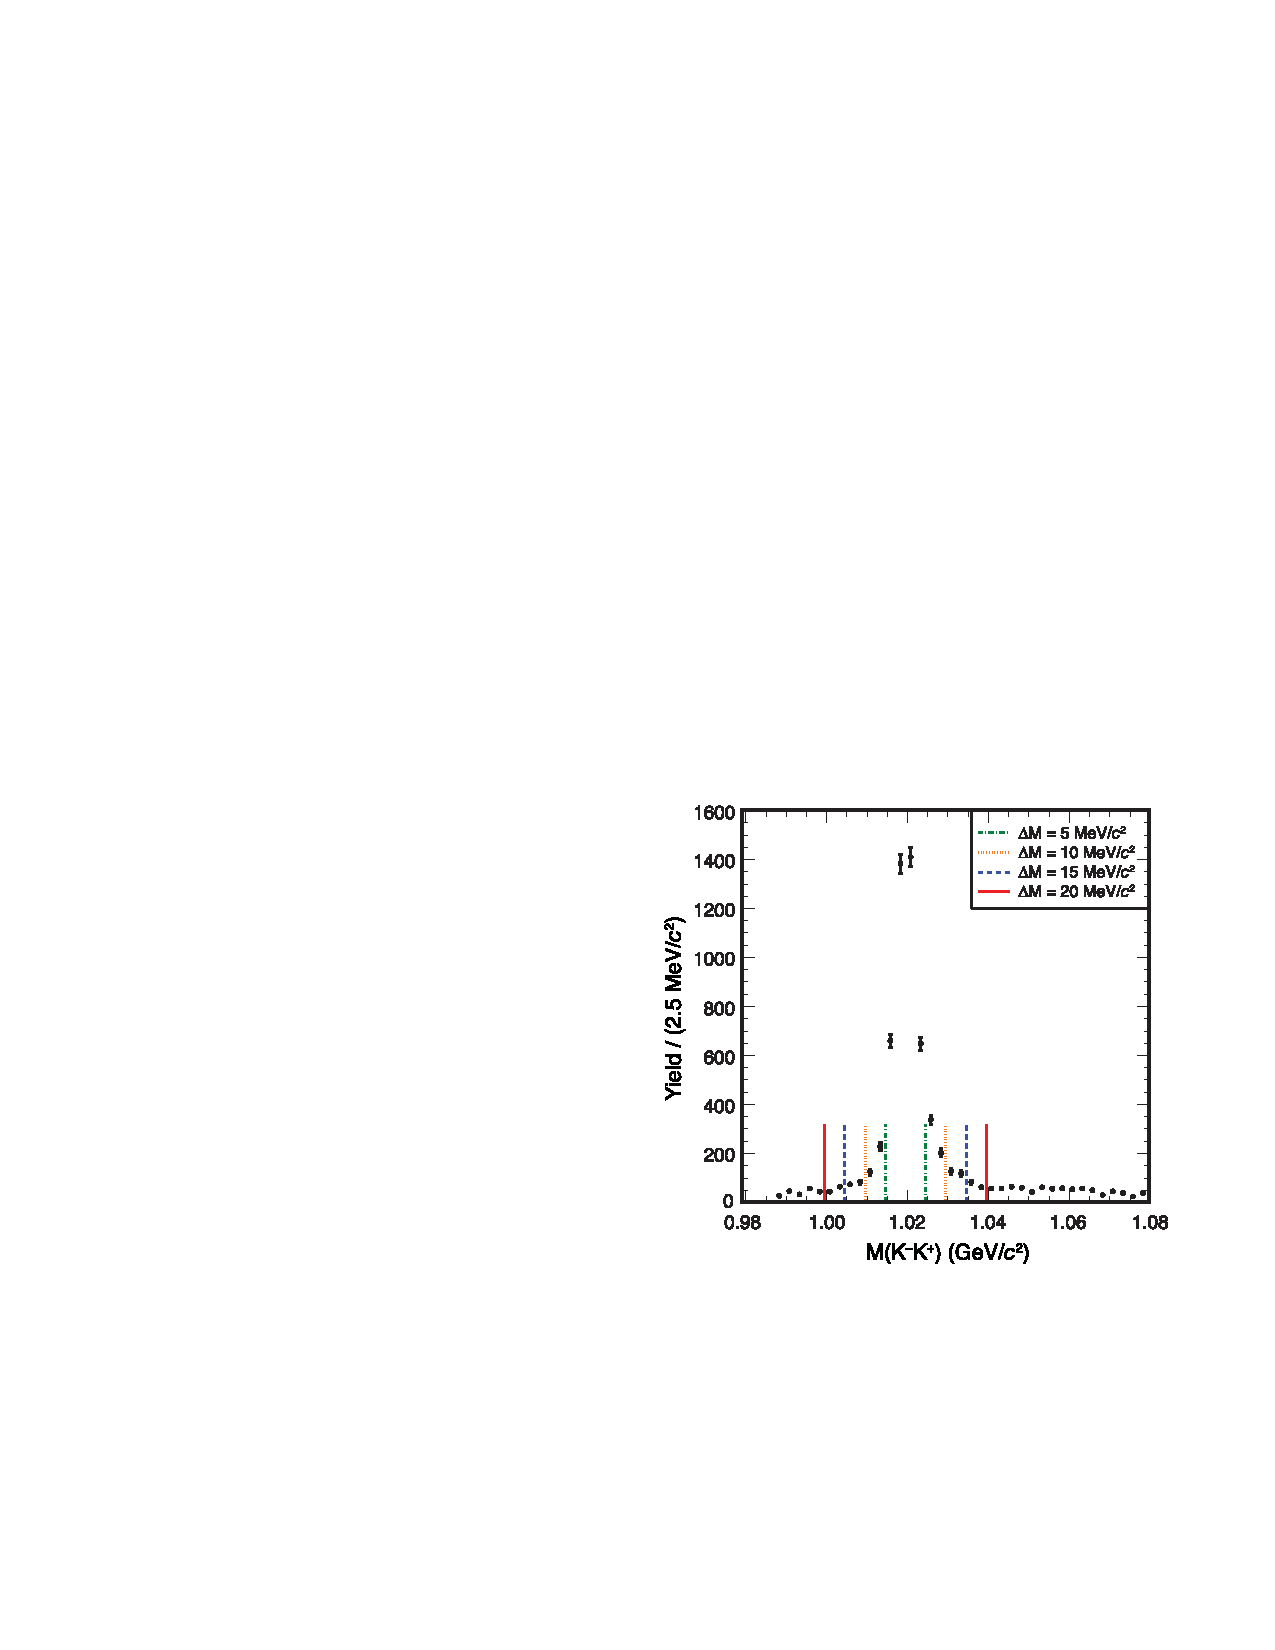
\includegraphics[width=\textwidth]{production/selection/cleo_phi_definition}
  \caption{%
    Definition of the $\PKminus\PKplus$ mass windows used by the \cleo\ 
    collaboration to measure \DspTophipi branching 
    fractions~\cite{Alexander:2008aa}.
    The $\PKminus\PKplus$ mass window used in the charm production measurement 
    corresponds to the window delimited by the solid red lines in the figure.
  }
  \label{fig:sel:offline:cleo_phi}
\end{figure}

The charm candidate invariant mass distributions after the full offline 
selection after given in 
\cref{fig:prod:sel:D0ToKpi:offline,fig:prod:sel:DpToKpipi:offline,fig:prod:sel:DsToKKpi:offline,fig:prod:sel:DstToD0pi_D0ToKpi:offline}.
The number of charm candidates before and after the offline requirements are 
given in \cref{tab:prod:sel:candidates}.

\begin{figure}
  \begin{subfigure}[b]{0.5\textwidth}
    \centering
    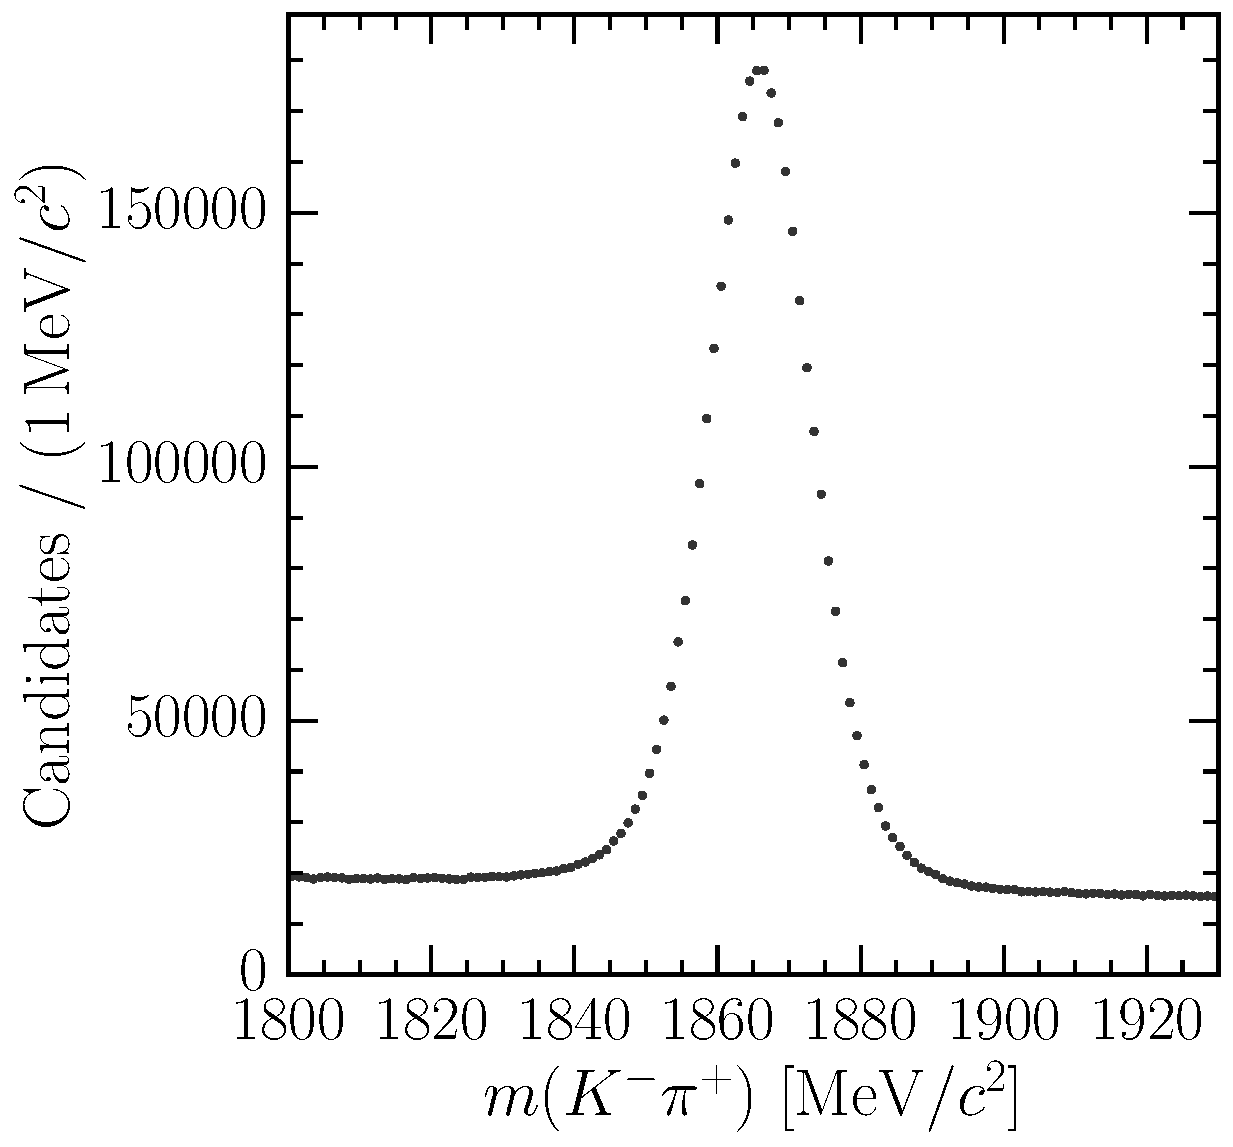
\includegraphics[width=\textwidth]{production/selection/D0ToKpi_mass}
    \caption{Online selected}
    \label{fig:prod:sel:D0ToKpi:online}
  \end{subfigure}
  \begin{subfigure}[b]{0.5\textwidth}
    \centering
    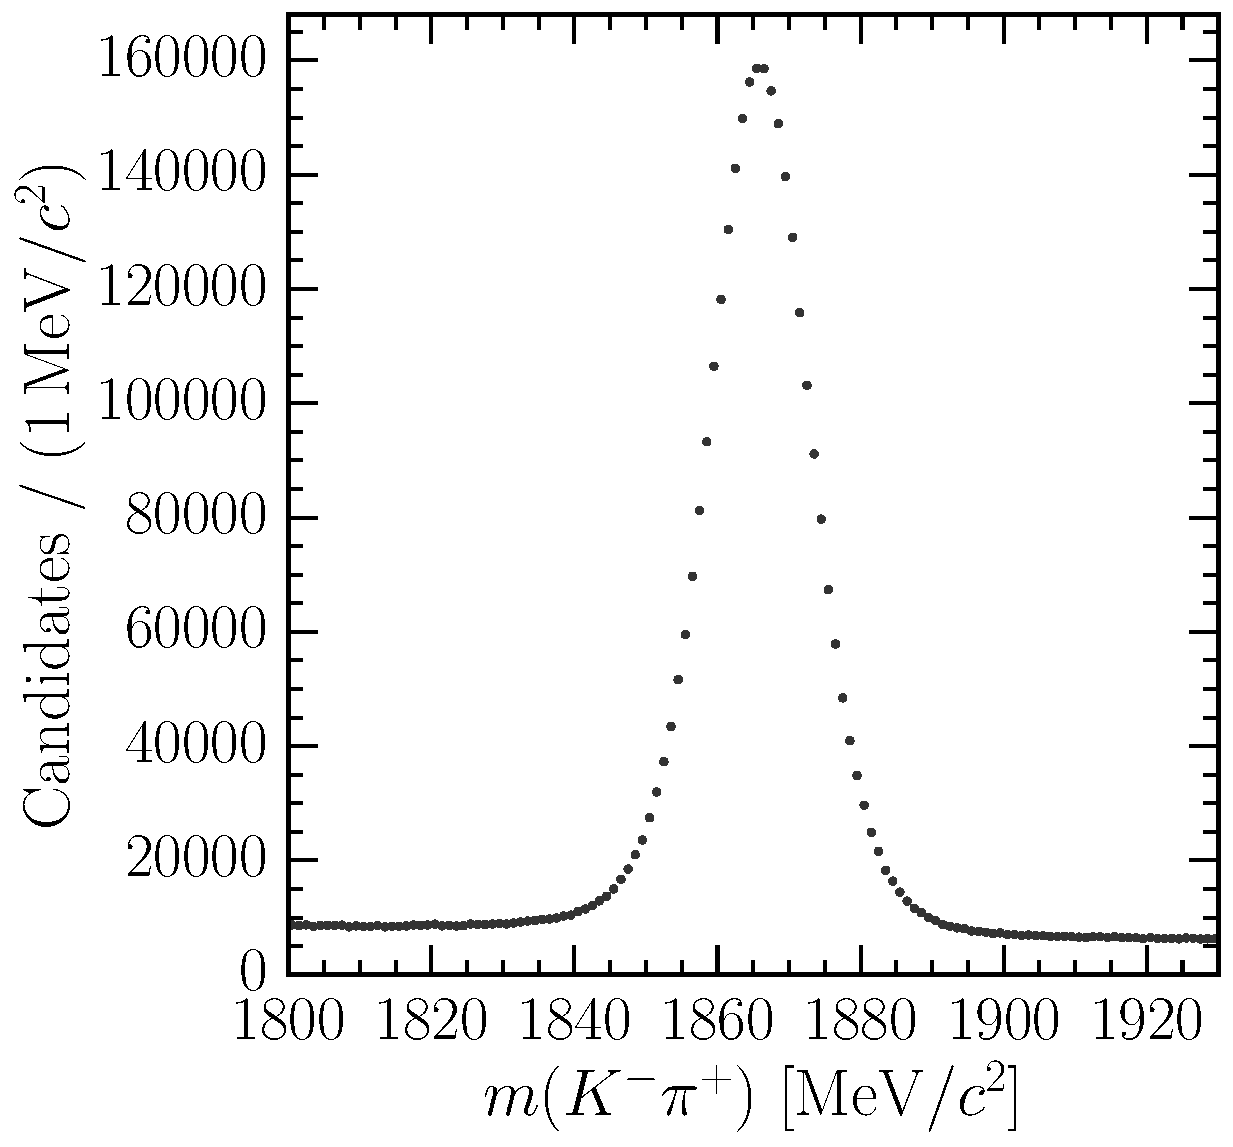
\includegraphics[width=\textwidth]{production/selection/D0ToKpi_mass_offline_selection}
    \caption{Offline selected}
    \label{fig:prod:sel:D0ToKpi:offline}
  \end{subfigure}
  \caption{%
    Mass distributions of \DzToKpi\ candidates after the online (trigger) 
    selection (\subref*{fig:prod:sel:D0ToKpi:online}) and after the offline 
    selection (\subref*{fig:prod:sel:D0ToKpi:offline}).
  }
  \label{fig:prod:sel:D0ToKpi}
\end{figure}

\begin{figure}
  \begin{subfigure}[b]{0.5\textwidth}
    \centering
    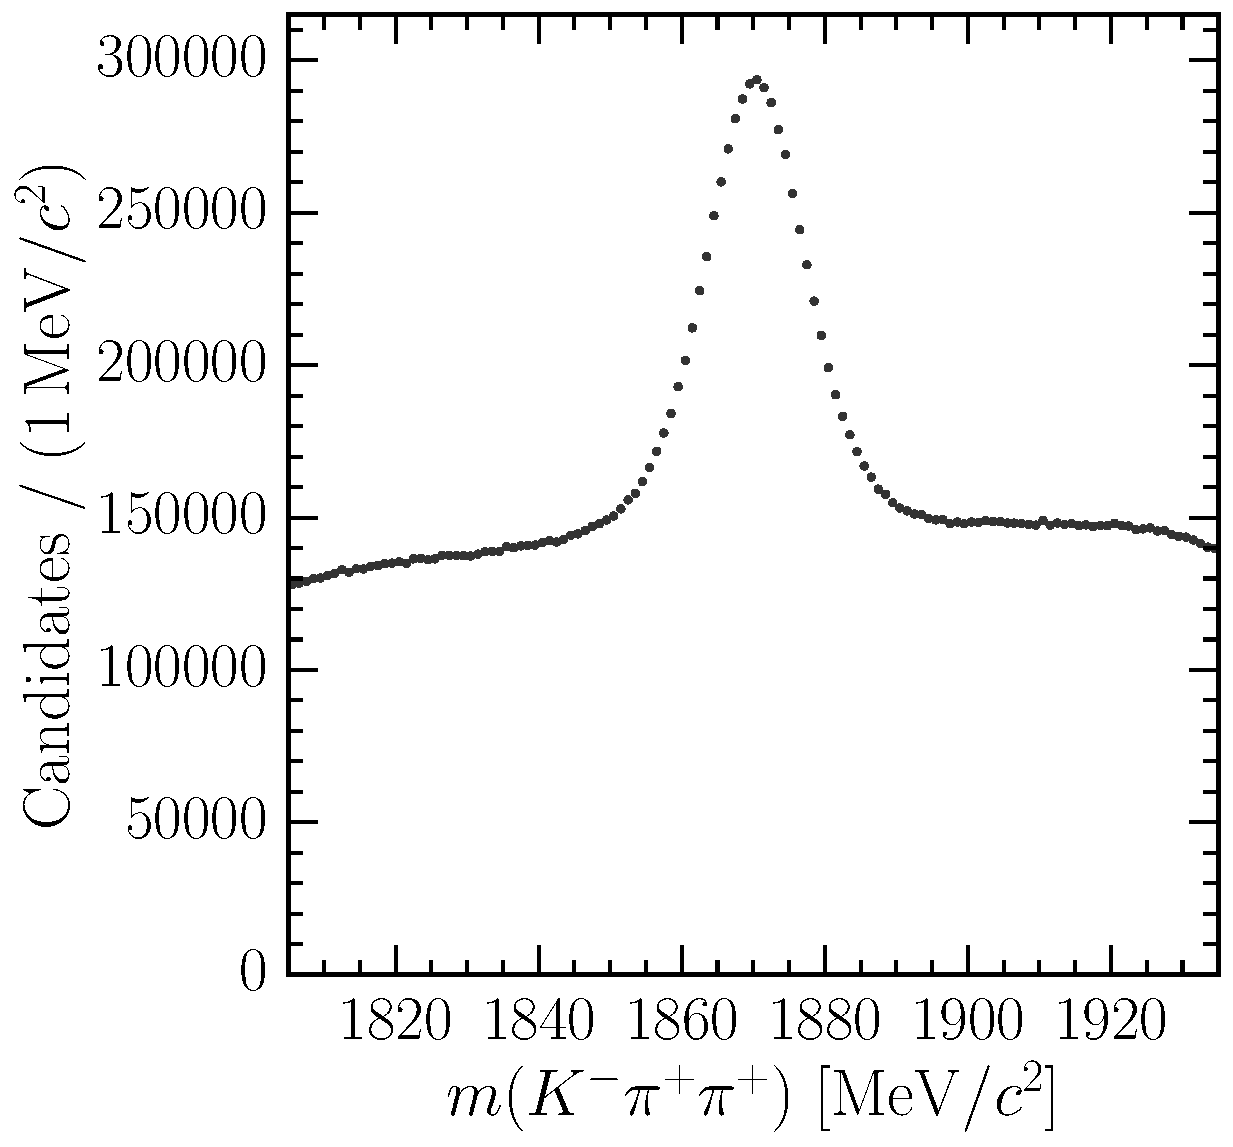
\includegraphics[width=\textwidth]{production/selection/DpToKpipi_mass}
    \caption{Online selected}
    \label{fig:prod:sel:DpToKpipi:online}
  \end{subfigure}
  \begin{subfigure}[b]{0.5\textwidth}
    \centering
    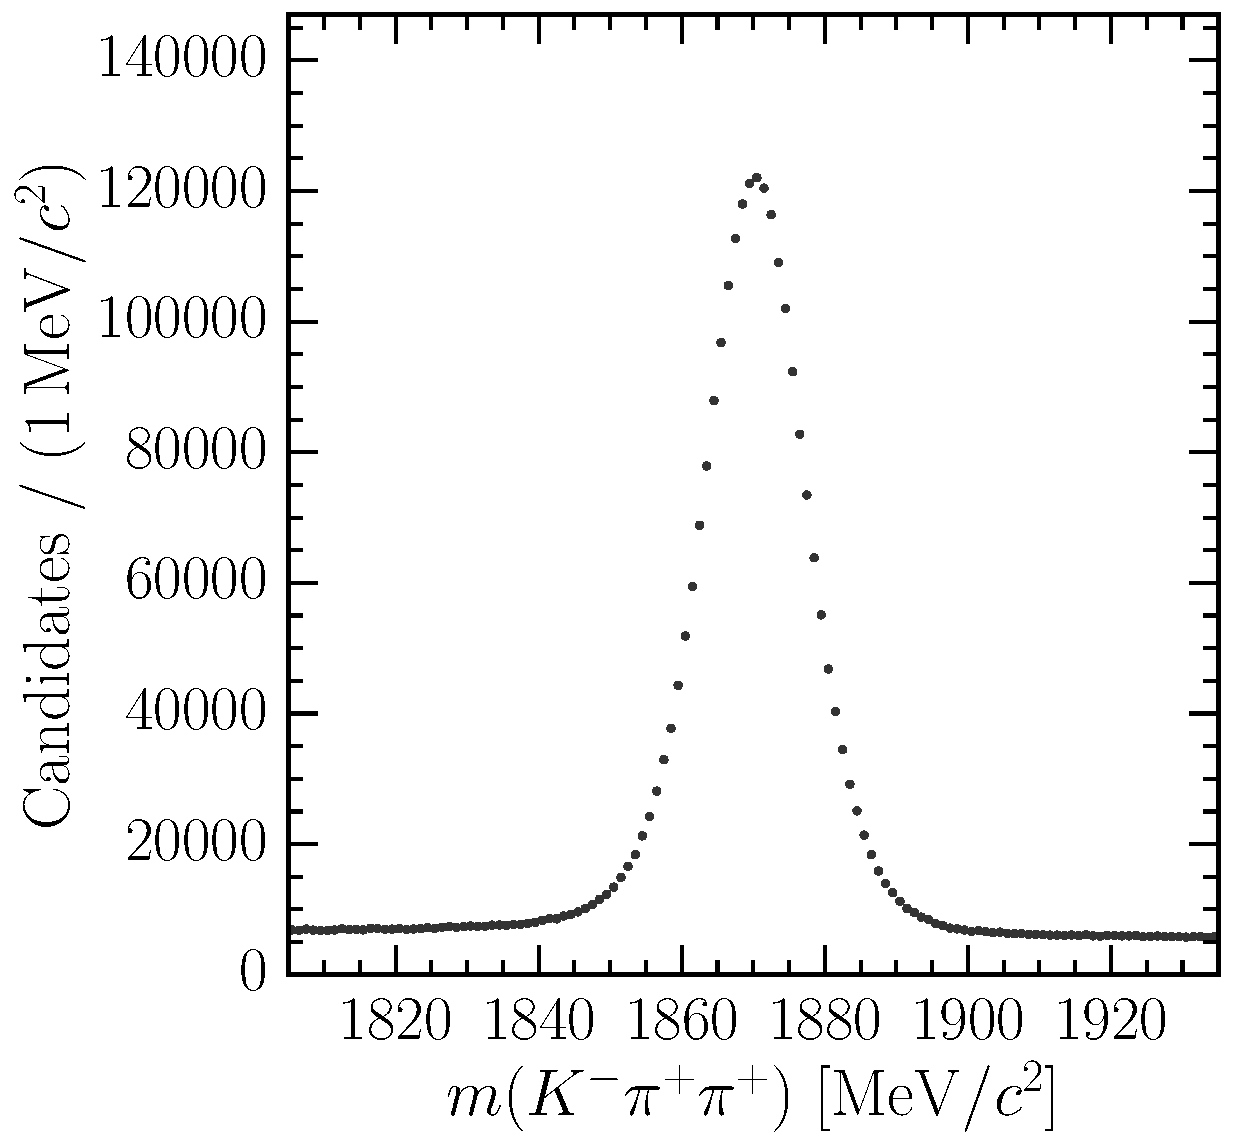
\includegraphics[width=\textwidth]{production/selection/DpToKpipi_mass_offline_selection}
    \caption{Offline selected}
    \label{fig:prod:sel:DpToKpipi:offline}
  \end{subfigure}
  \caption{%
    Mass distributions of \DpToKpipi\ candidates after the online (trigger) 
    selection (\subref*{fig:prod:sel:DpToKpipi:online}) and after the offline 
    selection (\subref*{fig:prod:sel:DpToKpipi:offline}).
  }
  \label{fig:prod:sel:DpToKpipi}
\end{figure}

\begin{figure}
  \begin{subfigure}[b]{0.5\textwidth}
    \centering
    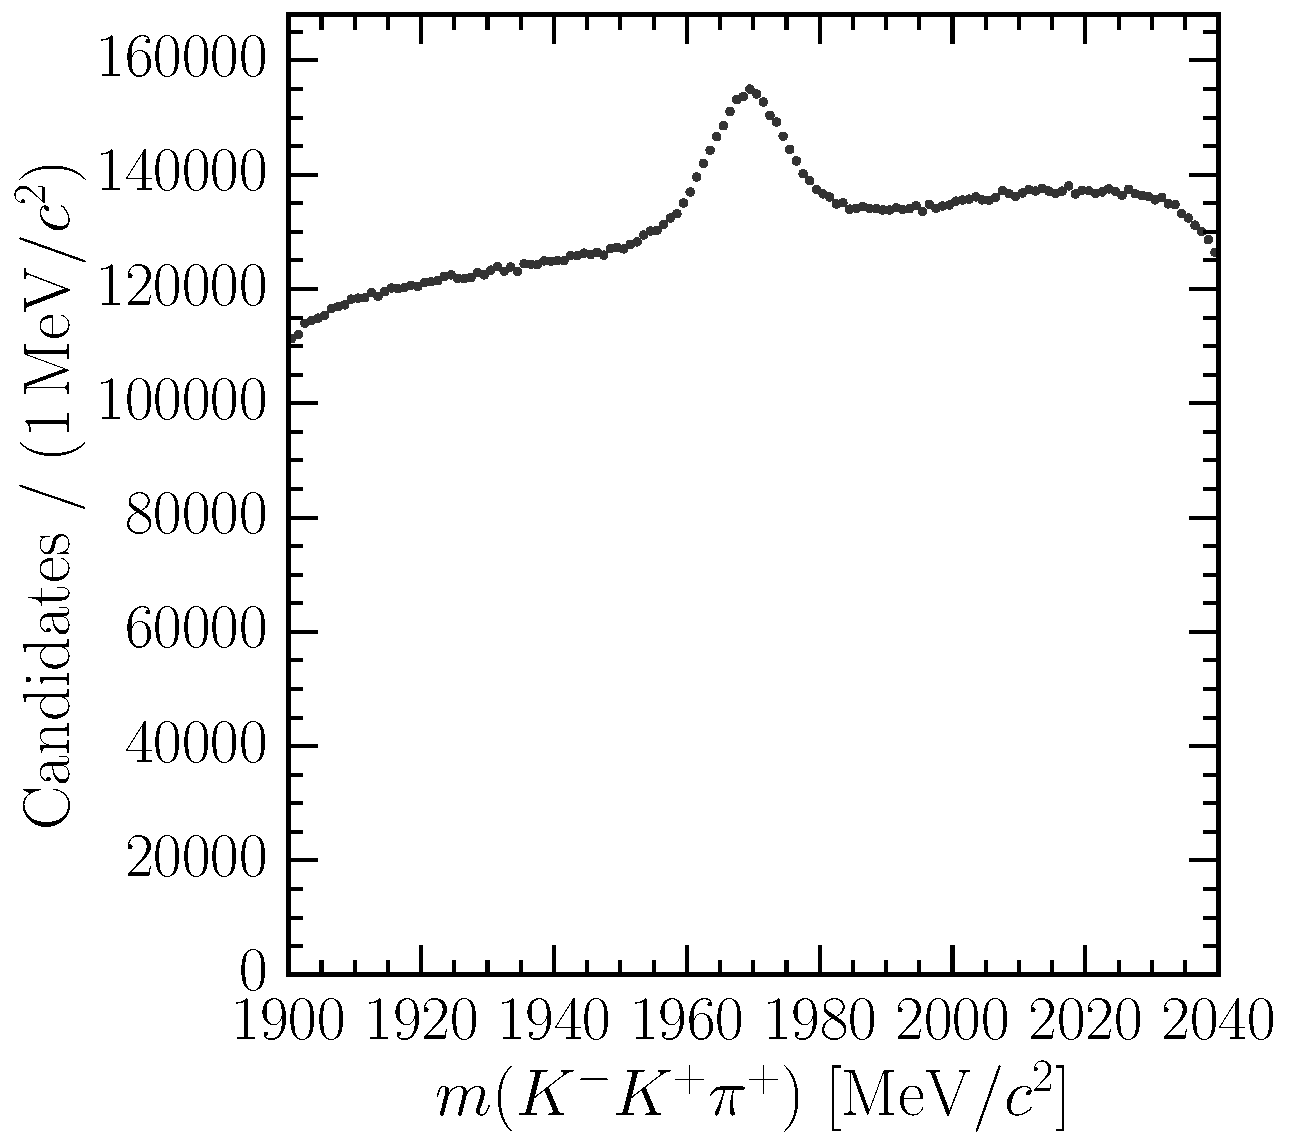
\includegraphics[width=\textwidth]{production/selection/DsToKKpi_mass}
    \caption{Online selected}
    \label{fig:prod:sel:DsToKKpi:online}
  \end{subfigure}
  \begin{subfigure}[b]{0.5\textwidth}
    \centering
    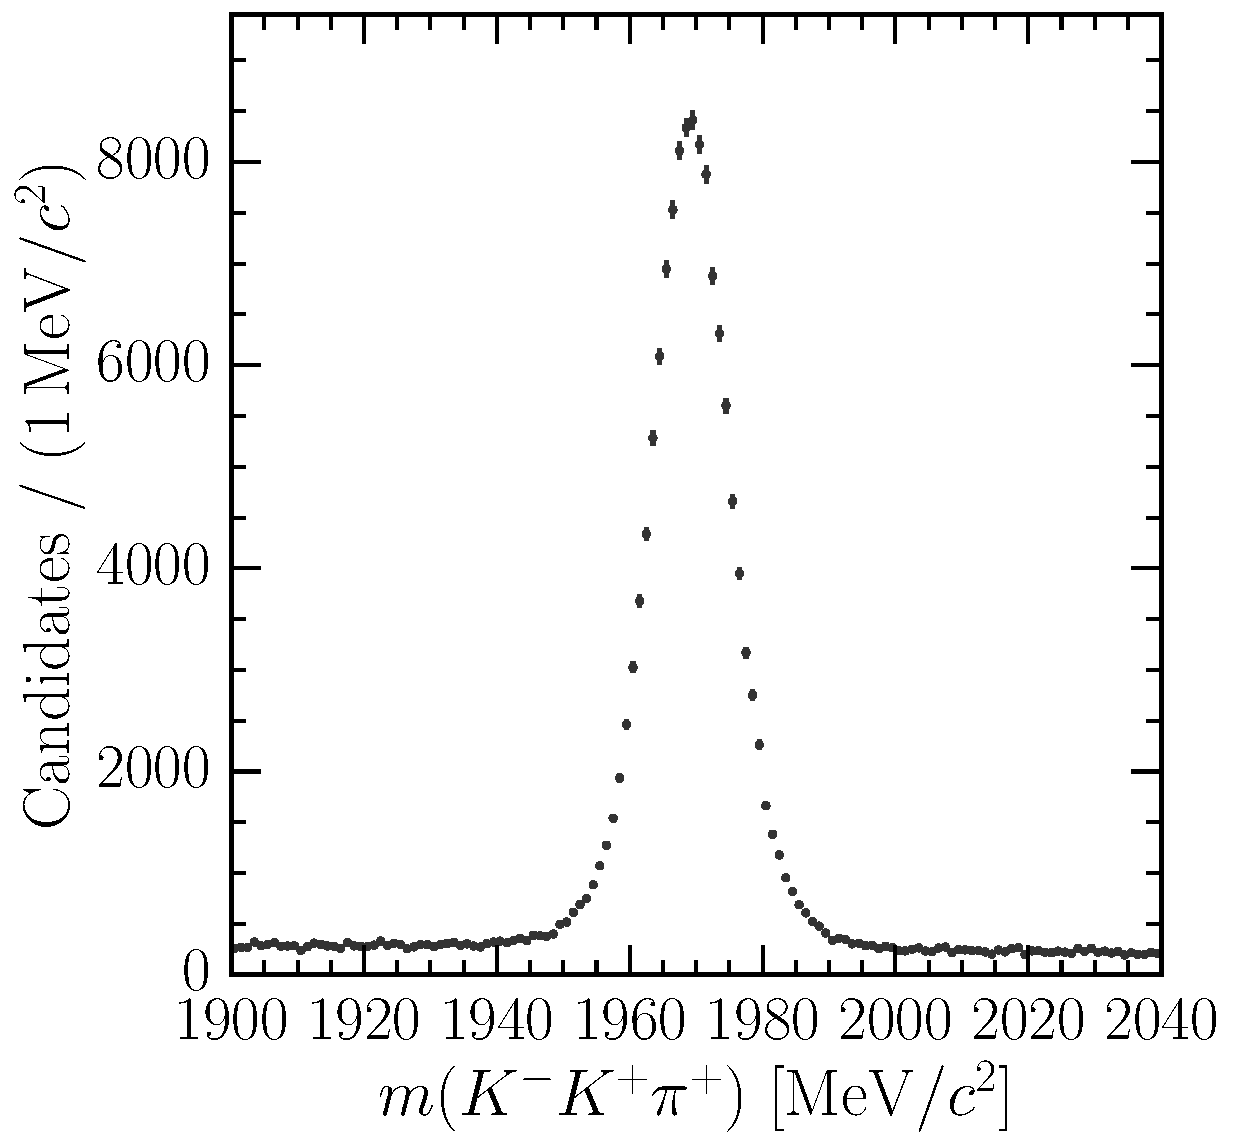
\includegraphics[width=\textwidth]{production/selection/DsToKKpi_mass_offline_selection}
    \caption{Offline selected}
    \label{fig:prod:sel:DsToKKpi:offline}
  \end{subfigure}
  \caption{%
    Mass distributions of \DspToKKpi\ candidates after the online (trigger) 
    selection (\subref*{fig:prod:sel:DsToKKpi:online}) and after the offline 
    selection (\subref*{fig:prod:sel:DsToKKpi:offline}).
    The offline selection includes the requirement that the kaon pair are 
    within a $\pm\SI{20}{\MeVcc}$ window around the nominal $\phi(1020)$ mass.
  }
  \label{fig:prod:sel:DsToKKpi}
\end{figure}

\begin{figure}
  \begin{subfigure}[b]{0.5\textwidth}
    \centering
    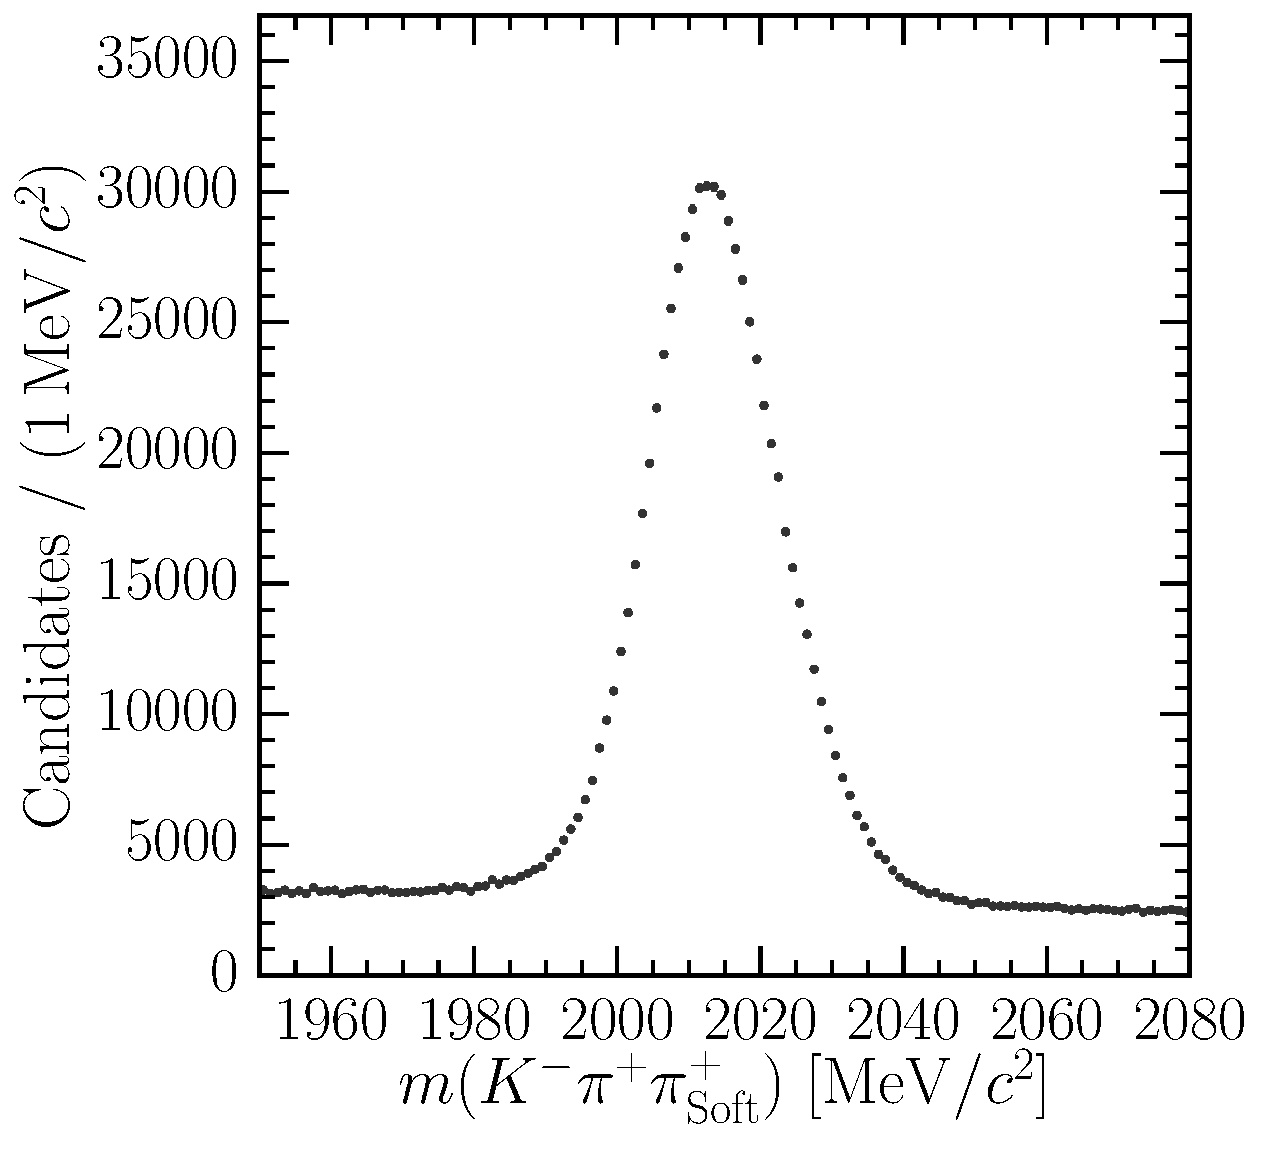
\includegraphics[width=\textwidth]{production/selection/DstToD0pi_D0ToKpi_mass}
    \caption{Online selected}
    \label{fig:prod:sel:DstToD0pi_D0ToKpi:online}
  \end{subfigure}
  \begin{subfigure}[b]{0.5\textwidth}
    \centering
    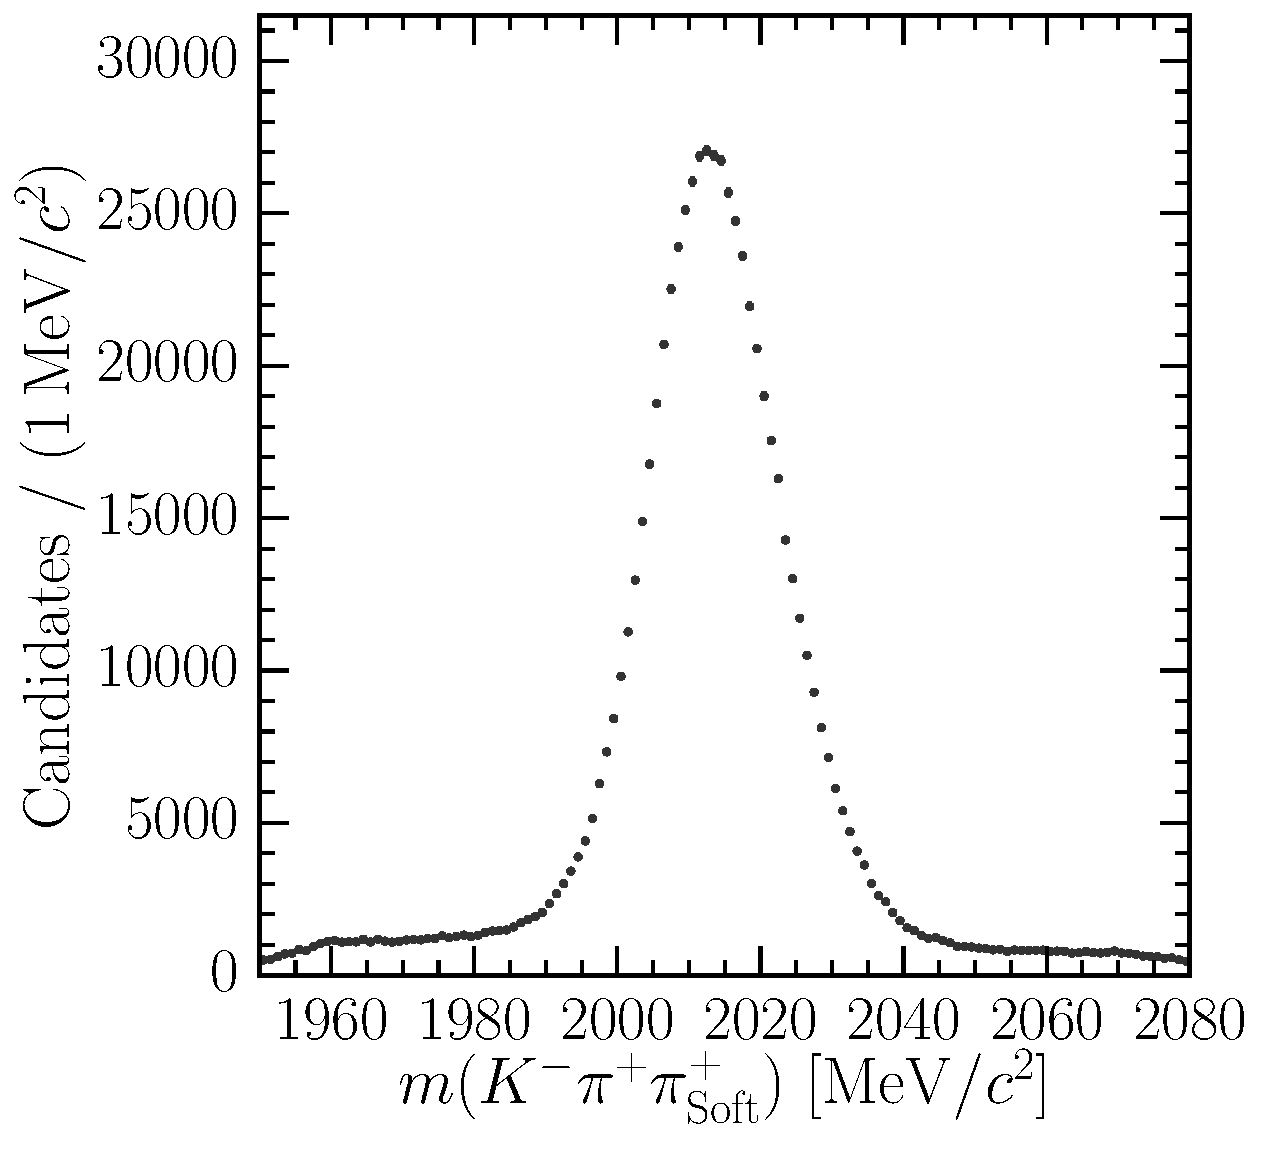
\includegraphics[width=\textwidth]{production/selection/DstToD0pi_D0ToKpi_mass_offline_selection}
    \caption{Offline selected}
    \label{fig:prod:sel:DstToD0pi_D0ToKpi:offline}
  \end{subfigure}
  \caption{%
    Mass distributions of \DstToDzpi\ candidates after the online (trigger) 
    selection (\subref*{fig:prod:sel:DstToD0pi_D0ToKpi:online}) and after the 
    offline selection (\subref*{fig:prod:sel:DstToD0pi_D0ToKpi:offline}).
  }
  \label{fig:prod:sel:DstToD0pi_D0ToKpi}
\end{figure}

\begin{table}
  \caption{%
    Number of candidates before and after the offline selection for each charm 
    candidate under study.
  }
  \label{tab:prod:sel:candidates}
  \centering
  \begin{tabular}{lccc}
  \toprule
  Decay mode & {$N_{\text{Online}}$} [\num{e6}] & {$N_{\text{Offline}}$} [\num{e6}] & {$N_{\text{Offline}}/N_{\text{Online}}$ (\%)} \\
  \midrule
  \DzToKpi   & 5.8 & 3.8 & 65 \\
  \DpToKpipi & 25  & 3.1 & 12 \\
  \DspToKKpi & 21  & 0.16 & 0.8 \\
  \DstToDzpi & 1.1 & 0.72 & 66 \\
  \bottomrule
\end{tabular}

\end{table}


\chapter{Yield extraction}
\label{chap:prod:fitting}

Signal charm mesons can be distinguished from combinatorial background in the 
invariant mass distribution of the vertex, as shown in 
\cref{fig:prod:sel:D0ToKpi:offline} for example.
However, the generating \acf{PDF} in this distribution is the same for both 
prompt and secondary charm, and so another distribution must be used to 
distinguish between these two sources of charm decays.

This analysis uses the natural logarithm of the \chisq\ of the \acf{IP}, 
\lnipchisq, to obtain the prompt charm yields.
The momentum vector of prompt charm should point back to the \acf{PV}, and so 
the \lnipchisq\ distribution is expected be centred around zero.
For secondary charm, the momentum vector will in general not point back to the 
\ac{PV}, and so the \lnipchisq\ distribution is expected to peak at higher 
values.
This separation is exploited to distinguish between prompt and secondary charm, 
where the prompt signal yield in each \pTy\ bin is measured by a binned 
\emph{maximum likelihood fit} to the \lnipchisq\ distribution, the general 
% Can't use \namecref here as it inserts 'Chapter' for some reason
formalism of which will be presented in the following Section.
The prompt and secondary models in this fit are described analytically as 
peaking functions.
The combinatorial background is described by a non-parametric model taken from 
the data outside the signal peak in the \emph{mass} distribution.
This background model is normalised in the \lnipchisq\ fit to the number of 
combinatorial background candidates in a signal window defined in the mass 
distribution, measured in a fit to the charm hadron mass spectrum.

For all cases but the \PDstarp\ measurement, it is the mass of the charm hadron 
that is used to discriminate all signal from combinatorial background.
For the \PDstarp\ measurement, the delta mass distribution, the difference 
\deltam\ between the reconstructed \PDstarp mass and the reconstructed \PDzero 
mass
\begin{equation}
  \deltam = m(\PKminus\Ppiplus\Ppiplussoft) - m(\PKminus\Ppiplus),
  \label{eqn:prod:fitting:delta_mass}
\end{equation}
is used instead.
This has a nominal value of \SI{145.4}{\MeVcc}~\cite{PDG2014}.
The narrower signal peak allows for a better signal-to-background ratio.

After an overview of the technique of maximum likelihood estimation is given, 
the two-step fit is described.
Firstly, a description of the parameterisation of the signal and combinatorial 
components in the mass and \deltam\ fits is given.
Secondly, the parameterisation of the prompt signal, secondary signal, and 
combinatorial background models in the \lnipchisq\ fit is given.
Specific details on the models used for each charm meson then follow, after 
which the fit results are presented.

\subsection{Maximum likelihood estimation}
\label{chap:prod:fitting:mle}

The technique used for the yield extraction is the method of maximum 
likelihood, where an objective function is defined that assumes some particular 
model truly generated the data.
The vector of parameters $\vec{\theta}$ of that model are varied given a vector 
$\vec{x}$ of $N$ independent, randomly distributed measurements $x_{i}$ until 
the objective is maximised.
This objective is the likelihood \likelihood, and is defined as
\begin{equation}
  \likelihood(\vec{\theta}|\vec{x}) = \prod_{i}^{N} f(x_{i}|\vec{\theta}),
\end{equation}
where $f$ is the \ac{PDF} that the data are assumed to have been sampled 
from.\footnotemark
Practically, it is useful to work with the logarithm of the likelihood, as sums 
are more convenient to work with numerically than products, and to use the 
negative of this, in order to be able to exploit the available numerical 
algorithms for minimisation problems such as \minuit~\cite{James:1975dr}
\begin{equation}
  -\ln{\likelihood(\vec{\theta}|\vec{x})} =
  -\sum_{i}^{N} \ln{f(x_{i}|\vec{\theta})}.
\end{equation}
This is the \acf{NLL}.
The practice of minimising the \ac{NLL} is also called \emph{fitting}.

\footnotetext{%
  The properties of any given \ac{PDF} $f(x)$ that are important here are: 
  $f(x) \geq 0$ for all $x$; and $\int_{-\infty}^{\infty} f(x)\dif{x} = 1$.
}

For the purposes of this analysis, the total \ac{PDF} $f$ is the sum of several 
models $f_{s}$, one for each physical source $s$ under consideration, such as 
signal and combinatorial background or different \pTy\ bins
\begin{equation}
  \ln{\likelihood(\vec{\theta}|\vec{x})} =
  \sum_{i}^{N} \ln{\sum_{s} f_{s}(x_{i}|\vec{\theta})}.
\end{equation}
The notation here that each model $f_{s}$ receives the full parameter vector 
$\vec{\theta}$ implies that each $f_{s}$ may share parameters with other 
components.
In order to not only model the shape of the components but also their absolute 
size, an \emph{extended} maximum likelihood fit~\cite{Barlow:1990vc} is 
performed that relaxes the normalisation requirement on the total \acp{PDF} to 
allow for Poisson fluctuations around the observed number of events 
$N_{\text{obvs.}}$
\begin{equation}
  \ln{\likelihood(\vec{\theta}, \vec{N}|\vec{x})} =
  \sum_{i}^{N}
    \ln{\sum_{s} N_{s}f_{s}(x_{i}|\vec{\theta})}
    - \sum_{s} N_{s}
  ,
\end{equation}
where $N_{s}$ is the \emph{yield} associated to each component model $f_{s}$ 
and $\vec{N}$ is the vector of those yields.

After defining the full model, the \acl{NLL} is minimised numerically using 
\minuit.
Minimising the \ac{NLL} is equivalent to finding the parameter vector 
$\hat{\theta}$ where the first derivatives of the likelihood with respect to 
each parameter are all zero
\begin{equation}
  \vec{u}(\vec{\theta}) = \frac{%
    \partial\ln{\likelihood}
  }{%
    \partial\vec{\theta}
  },\quad
  \vec{u}(\hat{\theta}) = \vec{0},
\end{equation}
where for compactness $\vec{\theta}$ includes the $\vec{N}$ parameter vector.
The uncertainties on the parameters can be found by inspecting the diagonal 
terms of the covariance matrix, which can be computed numerically by inverting 
the \emph{observed} Fisher information matrix $I(\hat{\theta})$, defined via
\begin{equation}
  I(\vec{\theta}) = \frac{%
    \partial^{2}\ln{\likelihood}
  }{%
    \partial\vec{\theta}\partial\vec{\theta}'
  }.
\end{equation}
The second derivative around the likelihood can be thought of as describing the 
`peakiness' of the minimum, where a shallower peak corresponds to less 
certainty in the measurement of the parameter, and conversely a sharper peak 
corresponds to a greater certainty in the value at the minimum.
The computation of the set of second derivatives, and the proceeding matrix 
inversion to obtain the covariance matrix, is performed numerically from the 
minimised \ac{NLL} by the \hesse\ algorithm, part of \minuit.

To estimate the yields in the data, suitable models must be constructed.
The following Sections shall describe the construction of these models for the 
various fits.

\section{Signal-background discrimination}
\label{chap:prod:fitting:mass}

For each one-dimensional mass and \deltam\ fit, one PDF is defined per 
discriminatory species: signal and combinatorial background.
In both the mass and \deltam\ distributions, the prompt and secondary signal 
shapes are assumed to be identical, and for the \deltam\ fits the combinatorial 
background is assumed to be indistinguishable from \emph{random soft pion} 
backgrounds, where a true \PDzero is combined with a random track in the event.
The total \ac{PDF} is constructed as the sum of the per-species \acp{PDF}, each $f_{s}$, 
each weighted by the respective yield $N_{s}$
\begin{align}
  f(m) &= \frac{1}{\sum_{\textnormal{s}} N_{\textnormal{s}}}
          \sum_{\textnormal{s}} N_{\textnormal{s}}
          f_{\textnormal{s}}(m),\\
  f(\deltam) &= \frac{1}{\sum_{\textnormal{s}} N_{\textnormal{s}}}
                \sum_{\textnormal{s}} N_{\textnormal{s}}
                f_{\textnormal{s}}(\deltam).
\end{align}

For every mass fit, the background PDF $f_{\textnormal{Bkg.}}(m)$ is taken to 
be a first-order polynomial, and the signal PDF $f_{\textnormal{Sig.}}(m)$ is 
dependent on the charm hadron candidate, given in 
Section~\ref{chap:prod:fitting:details}.

The combinatorial and random soft pion background in the \deltam\ fits is 
modelled as an empirical threshold function of the (un-normalised) form
\begin{equation}
  % (dm - dm0)^A * exp(B*dm)
  R(x; \deltam_{0}, A, B) = e^{B\deltam}
    {(x - \deltam_{0})}^A,
\end{equation}
where $\deltam_{0}$ is the threshold value, fixed to the charged pion rest mass 
$m_{\Ppipm} = \SI{139.57}{\MeVcc}$~\cite{PDG2014}, and the parameter $B$ is 
fixed to zero.
The signal PDF in \deltam\ is the sum of three normal distributions, sharing a 
common mean but allowed to have different widths.

One mass or \deltam\ PDF, $f(m)$ or $f(\deltam)$, is constructed per \pTy\ bin, 
and the likelihood is formed as the product of these such that each PDF is 
fitted simultaneously when the \ac{NLL} is minimised.

\section{Prompt-secondary discrimination}
\label{chap:prod:fitting:ipchisq}

The prompt and secondary signal distributions are modelled by continuous, 
parametric \acp{PDF}.
% TODO: explain KDE?
Rather than attempting to parameterise the combinatorial background 
distribution, a \acf{KDE} \ac{PDF}~\cite{Poluektov:2014rxa}, or `template', is 
created from a histogram of the \lnipchisq\ distribution in the lower and upper 
sidebands of the reconstructed charm hadron mass.
In the case of the \PDstarp measurements, the data in the upper sideband of the 
\deltam\ distribution is used instead.
This approach assumes that the \lnipchisq\ shape in the signal region is the 
same as that in the sidebands, that is that the mass and \lnipchisq\ are 
uncorrelated in the background sample.

The signal region in each long-lived charm hadron mass distribution is defined 
as a \SI{40}{\MeVcc}-wide window centred on the nominal rest mass of the given 
charm hadron, taken to be $m_{\PDzero} = \SI{1864.84}{\MeVcc}$, $m_{\PDplus} = 
\SI{1869.61}{MeV}$, and $m_{\PDsplus} = \SI{1968.30}{\MeVcc}$~\cite{PDG2014}.
The lower sideband is a \SI{20}{\MeVcc}-wide window centred \SI{50}{\MeVcc} 
below the centre of the signal window, and the upper sideband is a 
\SI{20}{\MeVcc}-wide window centred \SI{50}{\MeVcc} above the centre of the 
signal window.
For the \PDstarp\ measurements, the signal region is defined as a window 
\SI{6}{\MeVcc} wide, centred on the nominal \deltam\ value of 
\SI{145.43}{\MeVcc}~\cite{PDG2014}.
The upper sideband, or just `sideband' as a lower sideband region is not 
defined in \deltam, is defined as the region from \SI{4.5}{\MeVcc} to 
\SI{9}{\MeVcc} above the centre of the signal region.
\Cref{fig:prod:fitting:regions:D0ToKpi,fig:prod:fitting:regions:DpToKpipi,fig:prod:fitting:regions:DsToKKpi,fig:prod:fitting:regions:DstToD0pi_D0ToKpi}
show the signal and sideband regions for each mode.

The integral of the \lnipchisq\ background template \ac{PDF} is constrained to 
be near the number of background candidates in the mass or \deltam\ signal 
region.
To avoid any complications due to correlations between the background template 
\ac{PDF} and the fitted data, only the data in signal region is used in the 
\lnipchisq\ fit.
For the \PDstarp\ measurements, this signal region requirement is made in both 
the \PDzero mass and the \deltam\ distributions.

For each one-dimensional \lnipchisq\ fit, we assign one \ac{PDF} $f_{s}$ per 
discriminatory species: prompt signal, secondary signal, and combinatorial 
background.
The total \acp{PDF} are constructed as the sum of per-species \acp{PDF}, 
each weighted by the respective yield $N_{s}$
\begin{equation}
  f(\lnipchisq) = \frac{1}{\sum_{\textnormal{s}} N_{\textnormal{s}}}
                  \sum_{\text{s}} N_{\text{s}}
                  f_{\text{s}}(\lnipchisq).
\end{equation}
The constraint on the background yield \nbkg\ is applied by multiplying the 
likelihood by a normal distribution in \nbkg, whose mean is the number of 
background candidates $N_{\text{Bkg}}$ measured by the mass fit and whose width 
is the uncertainty on $N_{\text{Bkg}}$ returned by the fitter.
This penalises the likelihood by reducing its value when the fitted \nbkg\ 
parameter is far away from the value found in the mass fit.

One \lnipchisq\ \ac{PDF}, $f(\lnipchisq)$, and background constraint is 
constructed per \pTy\ bin, and the likelihood is formed as the product of these 
such that each \ac{PDF} is fitted simultaneously when the negative 
log-likelihood is minimised.
The benefit of this construction is that some shape parameters can be shared 
across bins, reducing the uncertainty on the fit parameters.
Which parameters are shared across bins and which are fitted independently is 
dependent on the charm meson, and are enumerated in 
\cref{chap:prod:fitting:details}.

The prompt signal model $H$ in the \lnipchisq\ distribution is a modified 
normal distribution, where the width is allowed to be asymmetric with respect 
to the mean and the tails are described by exponential functions
\begin{equation}
  H(x; \mu, \sigma, \epsilon, \rho_{L}, \rho_{R}) =
  \begin{cases}
    \exp\left(\frac{\rho_{L}^{2}}{2} + \rho_{L}\frac{x - \mu}{(1 - 
    \epsilon)\sigma}\right) & x < \mu - (\rho_{L}\sigma(1 - 
        \epsilon)), \\
    \exp\left(-\left(\frac{x - \mu}{\sqrt{2}\sigma(1 - 
    \epsilon)}\right)^{2}\right) & \mu - (\rho_{L}\sigma(1 - \epsilon)) 
          \leq x < \mu, \\
    \exp\left(-\left(\frac{x - \mu}{\sqrt{2}\sigma(1 + 
    \epsilon)}\right)^{2}\right) & \mu \leq x < \mu + (\rho_{R}\sigma(1 + 
          \epsilon)), \\
    \exp\left(\frac{\rho_{R}^{2}}{2} - \rho_{R}\frac{x - \mu}{(1 + 
    \epsilon)\sigma}\right) & x \geq \mu + (\rho_{R}\sigma(1 + 
        \epsilon)),
  \end{cases}
  \label{eqn:prod:fitting:ipchisq:signal_model}
\end{equation}
where the parameter $\mu$ is the mode of the distribution, $\sigma$ is the 
average of the left and right widths, $\epsilon$ is the asymmetry between the 
left and right widths, and $\rho_{L(R)}$ is the exponent for the left (right) 
tail.
The secondary signal distribution is modelled by a normal distribution $G$ with 
mean $\mu$ and width $\sigma$
\begin{equation}
  G(x; \mu, \sigma) = \frac{1}{\sqrt{2\pi}\sigma}
                      e^{-\frac{{(x - \mu)}^{2}}{2\sigma^{2}}}.
\end{equation}
These shapes are motivated by the \lnipchisq\ distributions for prompt and 
secondary signal decays observed in the \ac{MC} samples.

Given the large number of parameters to be fitted, some shape parameters in the 
prompt and secondary singal \lnipchisq\ \acp{PDF} are fixed to values obtained 
from `prefits' to the pure samples of prompt and secondary signal \ac{MC} 
described in \cref{chap:prod:data:mc}.
The set of parameters that is fixed is dependent on the charm meson, given in 
\cref{chap:prod:fitting:details}.

\section{Mode-specific details}
\label{chap:prod:fitting:details}

As different final states exhibit different features in the mass, \deltam, and 
\lnipchisq\ distributions, several aspects of the fits are different between 
modes.
This \namecref{chap:prod:fitting:details} gives the list of parameters that are 
split between \pTy\ bins, and the list of parameters that are allowed to float 
after the \ac{MC} prefits, for each mode.

Initially, no knowledge is assumed on which parameters should be independent 
(to be `split') across the \pTy\ bins, nor of whether the \lnipchisq\ 
distribution is well-modelled by the \ac{MC}.
The chosen parameterisation is that which best describes the data.
For the mass fits, all parameters are initially fixed such that they are same 
across all \pTy\ bins, and are then split one by one when it is observed that a 
feature varies across the bins, such as the width of the signal peak.
All parameters of the \lnipchisq\ fits are first kept fixed to values found 
from the fits to the simulated data, and then individual parameters are floated 
if the total PDF does not model the data well.
Parameters are then split across \pTy\ bins in the same manner as in the mass 
fits.

\subsection{Fit details for \PDzero}
\label{chap:prod:fitting:details:D0ToKpi}

For the \DzToKpi\ mode, the signal shape in the mass fit is the sum of a normal 
and a Crystal Ball distribution~\cite{Skwarnicki:1986xj}, sharing a common mode 
but allowed to have different widths.
The Crystal Ball function $C$ is a normal distribution but with a power-law 
tail on one side, defined (un-normalised) as
\begin{equation}
  C(x; \mu, \sigma, \alpha, n) = \begin{cases}
    e^{-\frac{{(x - \mu)}^{2}}{2\sigma^{2}}}                          & \frac{x - \mu}{\sigma} > -\alpha, \\
    e^{-\frac{|\alpha|^{2}}{2}}
      {(\frac{n}{|\alpha|})}^{n}
      {(\frac{n}{|\alpha|} - |\alpha| - \frac{x - \mu}{\sigma})}^{-n} & \frac{x - \mu}{\sigma} \leq -\alpha,
  \end{cases}
  \label{eqn:prod:fitting:crystal_ball}
\end{equation}
where $\alpha$ defines how far away from the mode $\mu$ the power-law tail 
begins, in units of the width of the core Gaussian $\sigma$, and $n$ is the 
power law exponent.
The mode and width of the total signal mass \ac{PDF} are split across \pTy\ 
bins, as is the slope of the background mass \ac{PDF}.
The mode of the \lnipchisq\ prompt signal \ac{PDF} and the width of the 
secondary signal \ac{PDF} are also split across \pTy\ bins.
The mode and width of the prompt signal \lnipchisq\ \ac{PDF} and all parameters 
of the secondary signal \lnipchisq\ \ac{PDF} are floated in the fit to data, 
and all other \lnipchisq\ shape parameters are fixed to the values from 
\ac{MC}.

Prefits to the prompt signal and secondary signal data samples in \lnipchisq\ 
are given in \cref{fig:prod:fitting:prefits:D0ToKpi}.

\subsubsection*{Fit details for \PDplus}
\label{chap:prod:fitting:details:DpToKpipi}

For the \DpToKpipi\ mode, the signal shape in the mass fit is the sum of a 
normal and a Crystal Ball distribution, sharing a common mode but allowed to 
have different widths.
The mode of the signal mass \ac{PDF} as well as the width of the Crystal Ball 
component in the mass \ac{PDF} are split across \pTy\ bins, as is the slope of 
the background mass \ac{PDF}.
The mode of the \lnipchisq\ prompt signal and secondary signal distributions 
are split across \pTy\ bins.
The mode and tail parameters of the signal \lnipchisq\ \ac{PDF}, are floated 
during the fit to data, with all other shape parameters fixed to the values 
from \ac{MC}.

Prefits to the prompt signal and secondary signal data samples in \lnipchisq\ 
are given in \cref{fig:prod:fitting:prefits:DpToKpipi}.

\subsubsection*{Fit details for \PDsplus}
\label{chap:prod:fitting:details:DsToKKpi}

For the \DspTophipi\ mode, the signal shape in the mass fit is the sum of a two 
normal distributions, sharing a common mean but allowed to have different 
widths.
The mean and width of the signal mass \ac{PDF} and the slope of the background 
mass \ac{PDF}, along with the mode of the \lnipchisq\ prompt signal \ac{PDF}, 
are split across \pTy\ bins.
The mode of the prompt signal \lnipchisq\ \ac{PDF} and all parameters of the 
secondary \ac{PDF} are floated during the fit to data, with all other shape 
parameters fixed to the values from \ac{MC}.

Prefits to the prompt signal and secondary signal data samples in \lnipchisq\ 
are given in \cref{fig:prod:fitting:prefits:DsToKKpi}.

\subsubsection*{Fit details for \PDstarp}
\label{chap:prod:fitting:details:DstToD0pi}

For the \PDstarp-tagged \DzToKpi\ mode, the width of the widest component of 
the signal model, described in \cref{chap:prod:fitting:mass}, is split across 
\pTy\ bins, along with the mean of the prompt signal \lnipchisq\ \ac{PDF}.
The mean of the prompt signal \lnipchisq\ \ac{PDF} and all parameters of the 
secondary \ac{PDF} are floated during the fit to data, with all other shape 
parameters fixed to the values from \ac{MC}.

Prefits to the prompt signal and secondary signal data samples in \PDzero 
\lnipchisq\ are given in \cref{fig:prod:fitting:prefits:DstToD0pi_D0ToKpi}.

\subsection{Fit results}
\label{chap:prod:fitting:results}

For all fits, the covariance matrix is checked to be positive definite, and the 
goodness-of-fit within each \pTy\ bin is checked visually to ensure that the 
\ac{NLL} minimisation stopped at a sensible parameter value set.
Mass, \deltam, and \lnipchisq\ fits are given in 
\cref{fig:prod:fitting:D0ToKpi,fig:prod:fitting:DpToKpipi,fig:prod:fitting:DsToKKpi,fig:prod:fitting:DstToD0pi_D0ToKpi}, 
where the data and models shown are the sums of the data and models over all 
\pTy\ bins.
Prompt signal yields per \pTy\ bin are given in 
\cref{tab:prod:fitting:D0ToKpi,tab:prod:fitting:DpToKpipi,tab:prod:fitting:DsToKKpi,tab:prod:fitting:DstToD0pi_D0ToKpi}, 
and those integrated across all bins in \cref{tab:prod:fitting:integrated}.

The plots show that the models match the data well, but there are some 
significant discrepancies such as in 
\cref{fig:prod:fitting:DsToKKpi:ipchisq,fig:prod:fitting:DstToD0pi_D0ToKpi:delta_mass}.
However, the discrepancies in these integrated plots are exaggerations of those 
in the individual \pTy\ bin fits: they indicate that there is a consistent bias 
in the individual bins, but do not necessarily indicate that these are 
statistically significant.
For comparison, 
\cref{fig:prod:fitting:D0ToKpi:sig_bkg,fig:prod:fitting:DpToKpipi:sig_bkg,fig:prod:fitting:DsToKKpi:sig_bkg,fig:prod:fitting:DstToD0pi_D0ToKpi:sig_bkg} 
show the mass (or \deltam) and \lnipchisq\ fits for each meson in the \pTy\ bin 
with the highest prompt signal yield and in the \pTy\ bin with the highest 
combinatorial background yield.
These show that, in the individual \pTy\ bins, the fits model the data 
significantly better than the integrated plots would suggest, and also that the 
fit is flexible enough to model both high prompt signal and high combinatorial 
background datasets.
The effect of the cross-section measurements of mis-modelling will be discussed 
further in \cref{chap:prod:syst:fitting}.

In some \pTy\ bins, it is not possible to make a prompt signal yield 
measurement due to insufficient data in those bins.
At this stage in the analysis, a cross-section measurement in a bin is 
considered infeasible if there is either no data (zero candidates), or if the 
prompt signal yield $N_{i} \pm \sigma_{N_{i}}$ in that bin as determined in the 
fit does not satisfy $N_{i} > 3\sigma_{N_{i}}$.

\begin{figure}
  \centering
  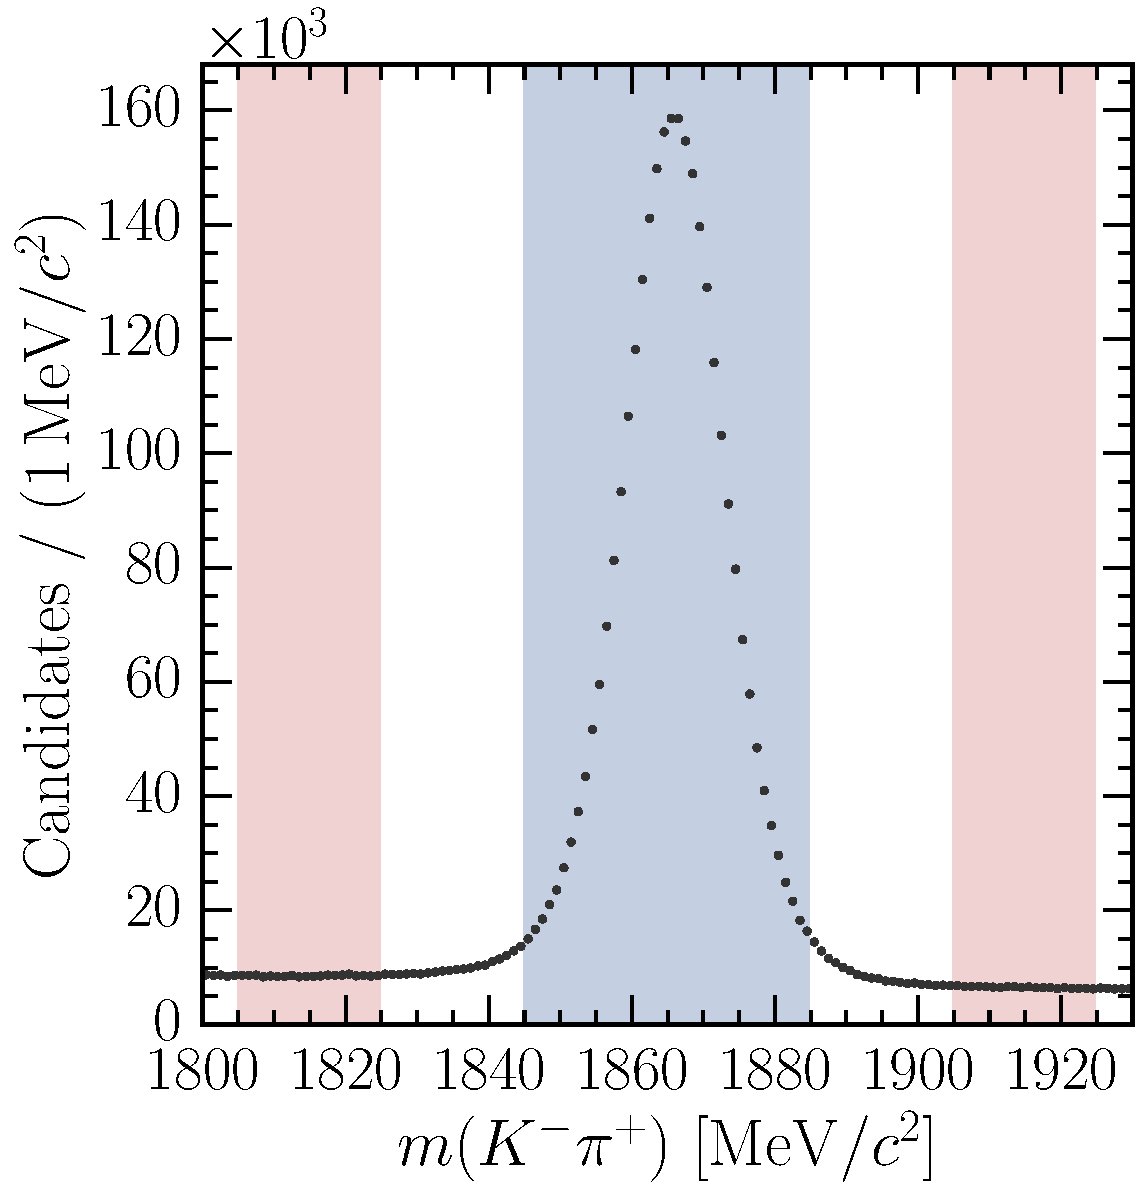
\includegraphics[width=\textwidth]{production/fitting/D0ToKpi_mass_offline_selection_regions}
  \caption{%
    Definition of signal window, in blue, and sidebands, in red, for \DzToKpi\ 
    candidates.
    The signal window is $\pm\SI{20}{\MeVcc}$ either side of the nominal 
    \PDzero mass of \SI{1864.84}{\MeVcc}~\cite{PDG2014}.
    The upper and lower sidebands are each \SI{20}{\MeVcc} wide, with the lower 
    sideband ending \SI{40}{\MeVcc} below the nominal \PDzero mass and the 
    upper sideband beginning \SI{40}{\MeVcc} above the nominal \PDzero mass.
    The full dataset is shown.
  }
  \label{fig:prod:fitting:regions:D0ToKpi}
\end{figure}

\begin{figure}
  \centering
  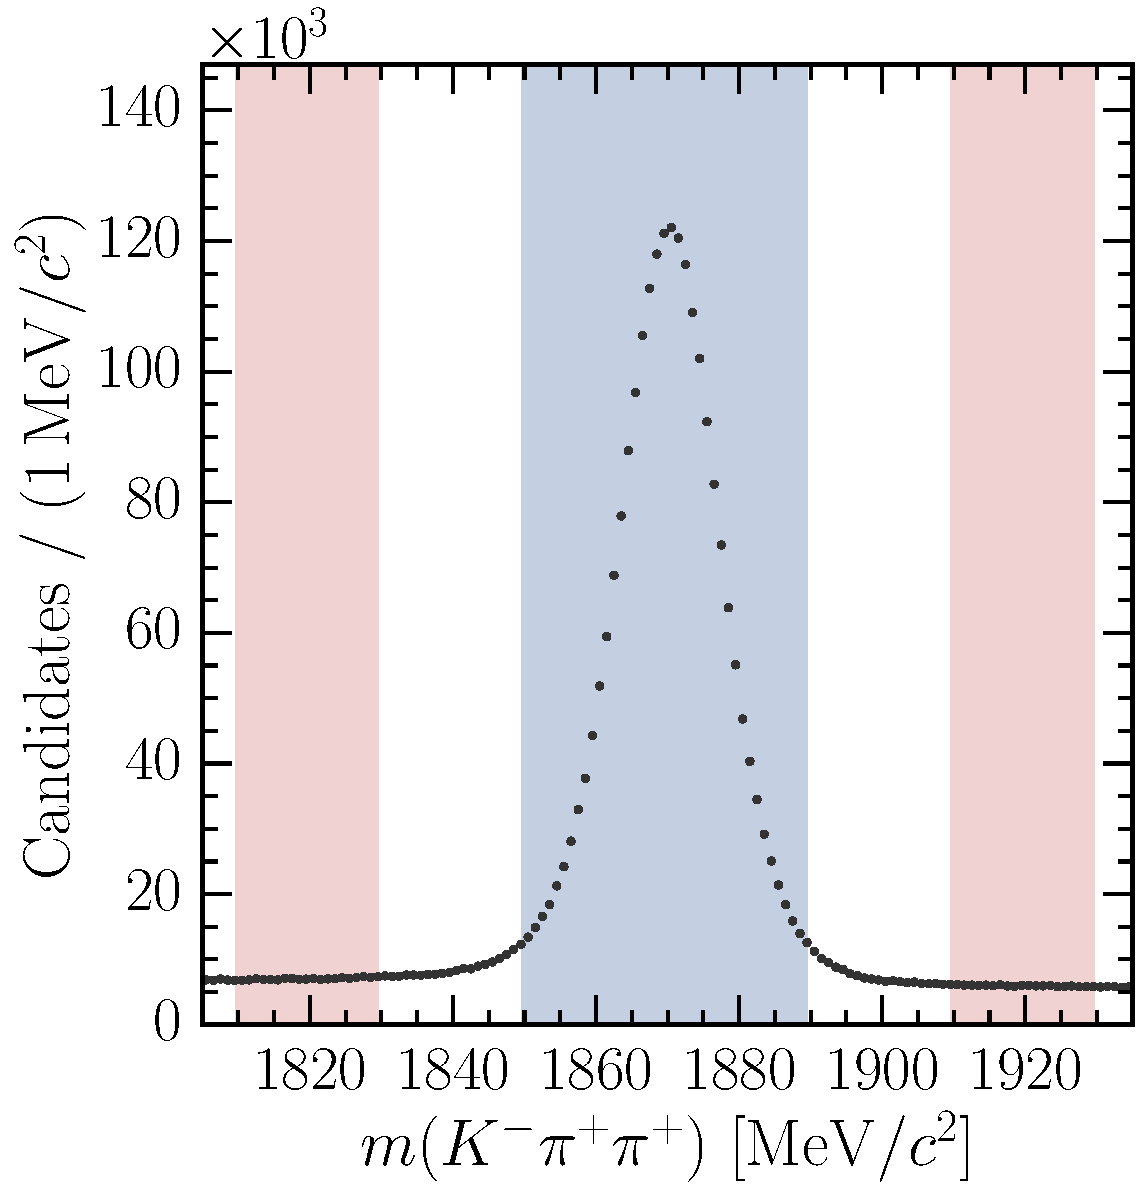
\includegraphics[width=\textwidth]{production/fitting/DpToKpipi_mass_offline_selection_regions}
  \caption{%
    Definition of signal window, in blue, and sidebands, in red, for 
    \DpToKpipi\ candidates.
    The signal window is $\pm\SI{20}{\MeVcc}$ either side of the nominal 
    \PDplus mass of \SI{1869.61}{\MeVcc}~\cite{PDG2014}.
    The upper and lower sidebands are each \SI{20}{\MeVcc} wide, with the lower 
    sideband ending \SI{40}{\MeVcc} below the nominal \PDplus mass and the 
    upper sideband beginning \SI{40}{\MeVcc} above the nominal \PDplus mass.
    The full dataset is shown.
  }
  \label{fig:prod:fitting:regions:DpToKpipi}
\end{figure}

\begin{figure}
  \centering
  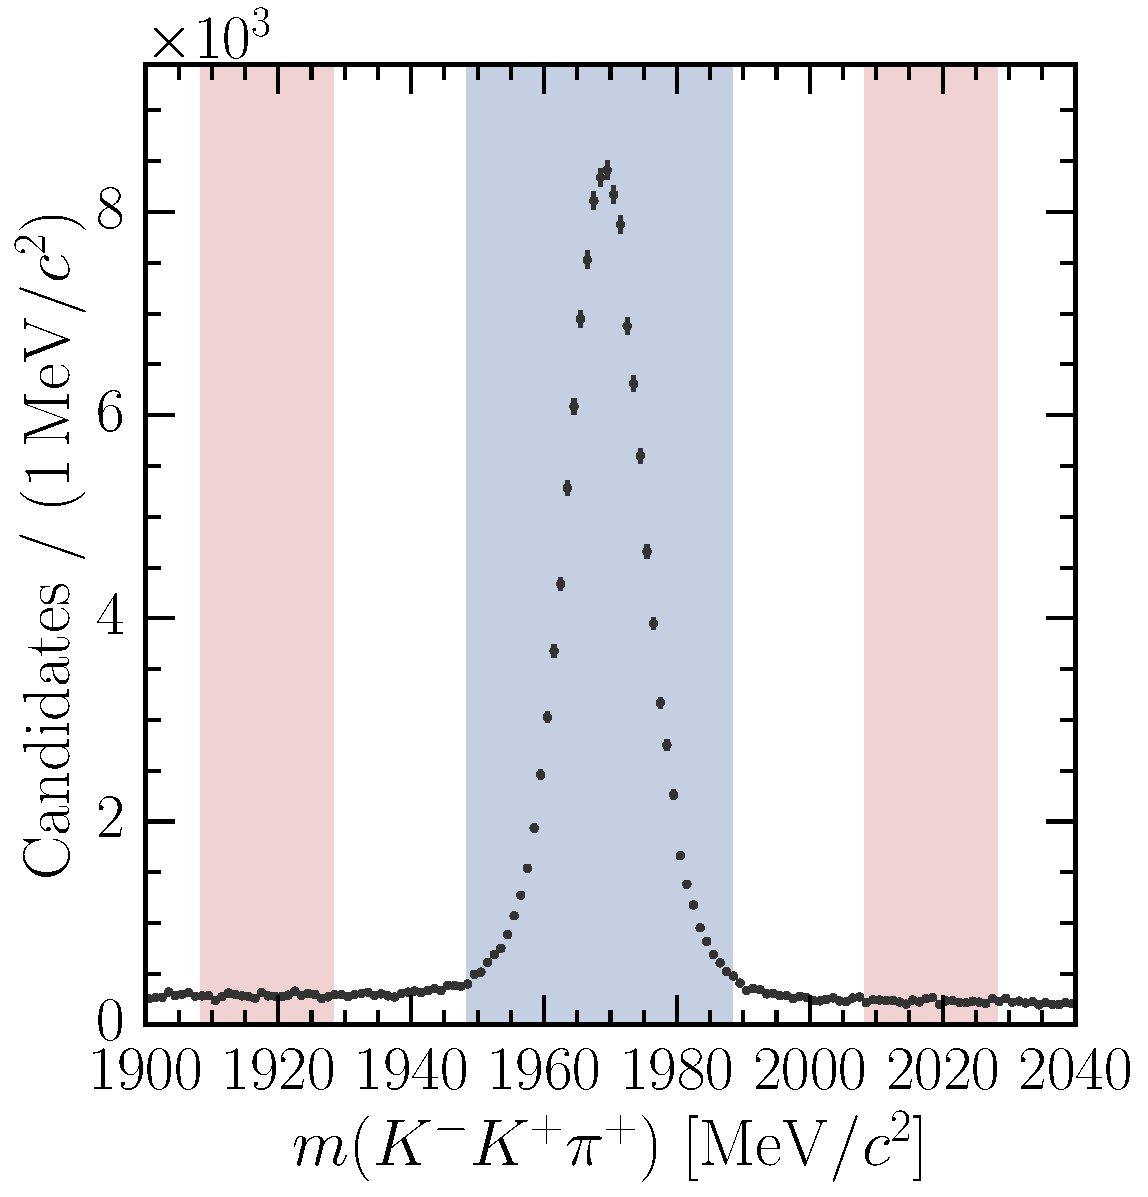
\includegraphics[width=\textwidth]{production/fitting/DsToKKpi_mass_offline_selection_regions}
  \caption{%
    Definition of signal window, in blue, and sidebands, in red, for 
    \DspTophipi\ candidates.
    The signal window is $\pm\SI{20}{\MeVcc}$ either side of the nominal 
    \PDsplus mass of \SI{1968.30}{\MeVcc}~\cite{PDG2014}.
    The upper and lower sidebands are each \SI{20}{\MeVcc} wide, with the lower 
    sideband ending \SI{40}{\MeVcc} below the nominal \PDsplus mass and the 
    upper sideband beginning \SI{40}{\MeVcc} above the nominal \PDsplus mass.
    The full dataset is shown.
  }
  \label{fig:prod:fitting:regions:DsToKKpi}
\end{figure}

\begin{figure}
  \centering
  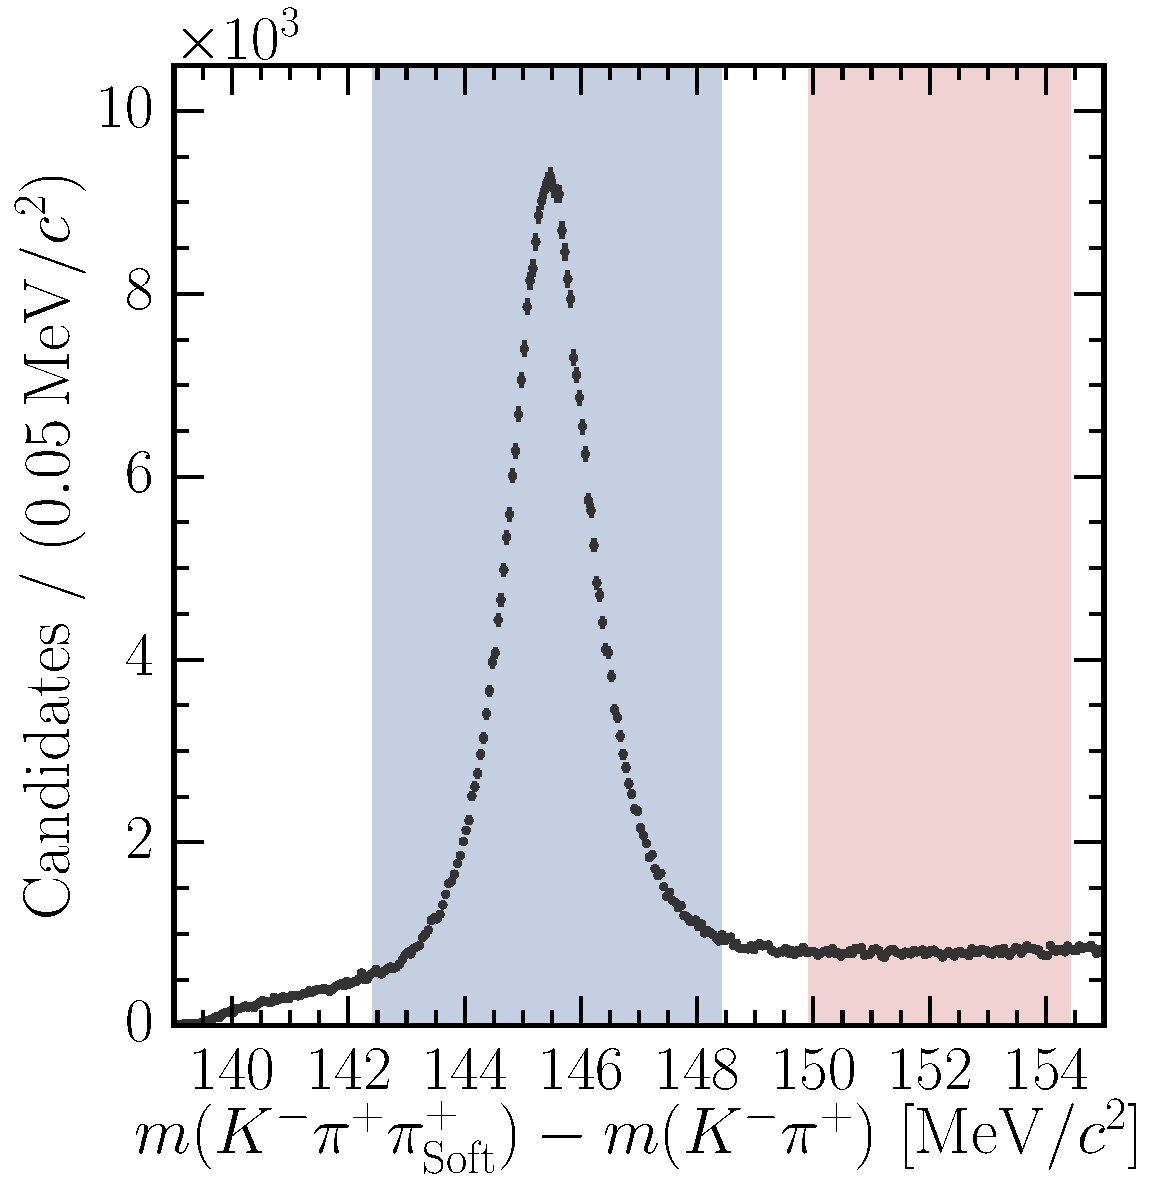
\includegraphics[width=\textwidth]{production/fitting/DstToD0pi_D0ToKpi_delta_mass_offline_selection_regions}
  \caption{%
    Definition of signal window, in blue, and sidebands, in red, for 
    \DstToDzpi, with \DzToKpi, candidates.
    The signal window is $\pm\SI{3}{\MeVcc}$ either side of the nominal 
    $\deltam = m(\PDstarp) - m(\PDzero)$ mass of 
    \SI{145.43}{\MeVcc}~\cite{PDG2014}.
    The upper sideband is \SI{4.5}{\MeVcc} wide, beginning \SI{4.5}{\MeVcc} 
    above the nominal \deltam\ value.
    The full dataset within the \PDzero signal region, given in 
    \cref{fig:prod:fitting:regions:D0ToKpi},is shown.
  }
  \label{fig:prod:fitting:regions:DstToD0pi_D0ToKpi}
\end{figure}

\begin{figure}
  \begin{subfigure}[b]{0.5\textwidth}
    \centering
    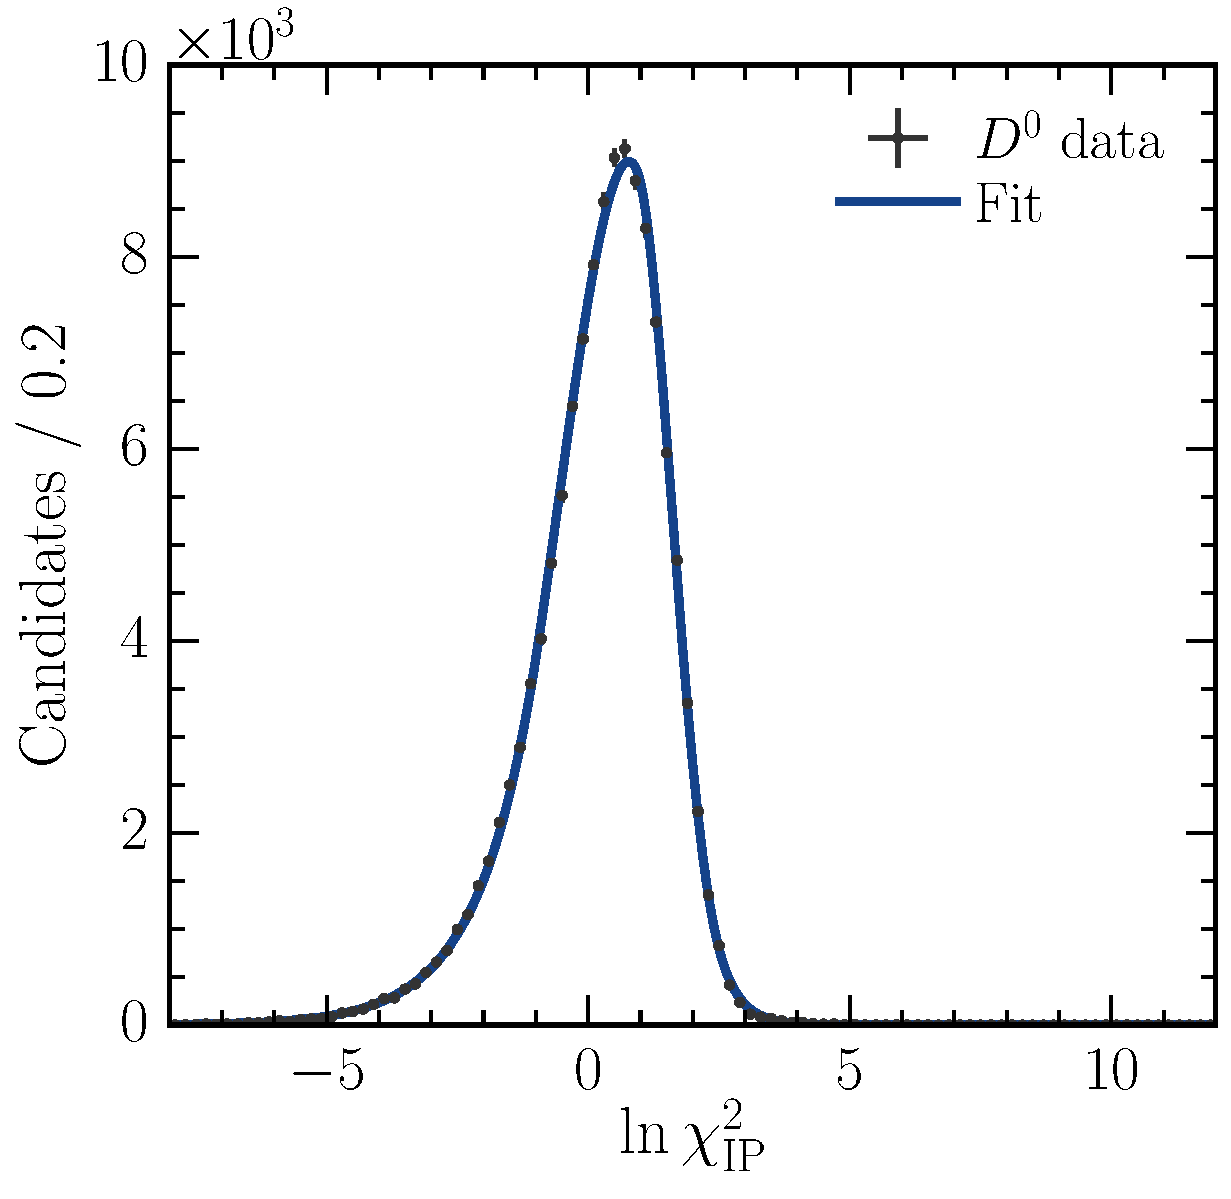
\includegraphics[width=\textwidth]{production/fitting/D0ToKpi_ipchisq_fit_pT_integrated_y_integrated_sig}
    \caption{Prompt}
    \label{fig:prod:fitting:prefits:D0ToKpi:prompt}
  \end{subfigure}
  \begin{subfigure}[b]{0.5\textwidth}
    \centering
    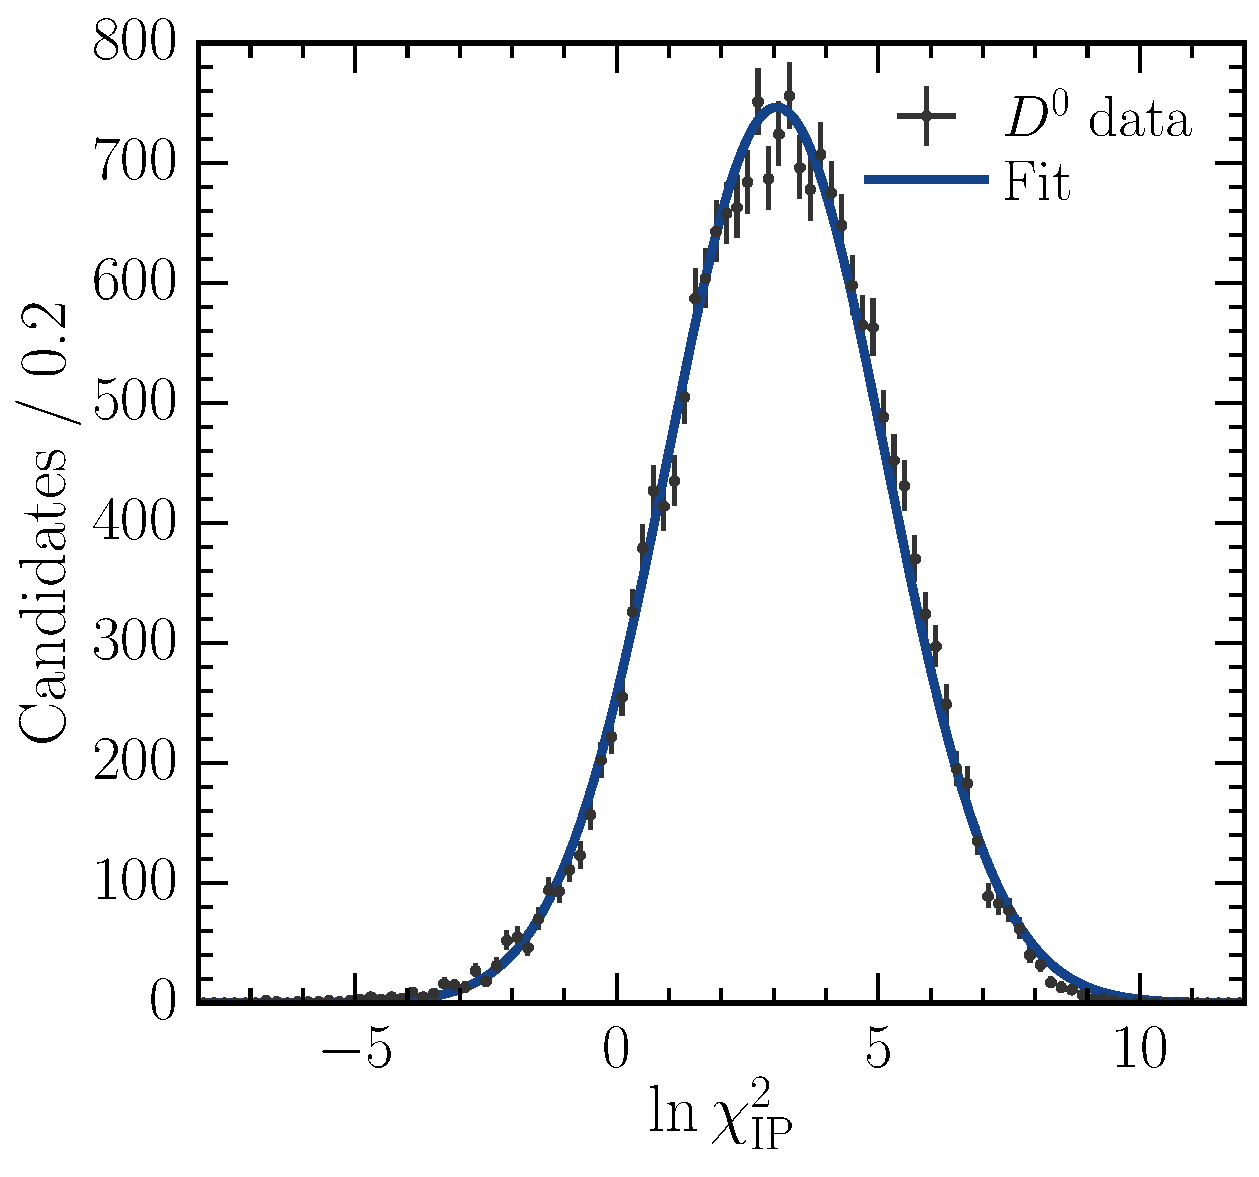
\includegraphics[width=\textwidth]{production/fitting/D0ToKpi_ipchisq_fit_pT_integrated_y_integrated_sec}
    \caption{Secondary}
    \label{fig:prod:fitting:prefits:D0ToKpi:secondary}
  \end{subfigure}
  \caption{%
    Distributions of \lnipchisq\ for simulated \DzToKpi\ decays: prompt signal 
    \PDzero (\subref*{fig:prod:fitting:prefits:D0ToKpi:prompt}) and secondary 
    signal \PDzero (\subref*{fig:prod:fitting:prefits:D0ToKpi:secondary}).
    The sum of the simultaneous likelihood fits in each \pTy\ bin is overlaid.
  }
  \label{fig:prod:fitting:prefits:D0ToKpi}
\end{figure}

\begin{figure}
  \begin{subfigure}[b]{0.5\textwidth}
    \centering
    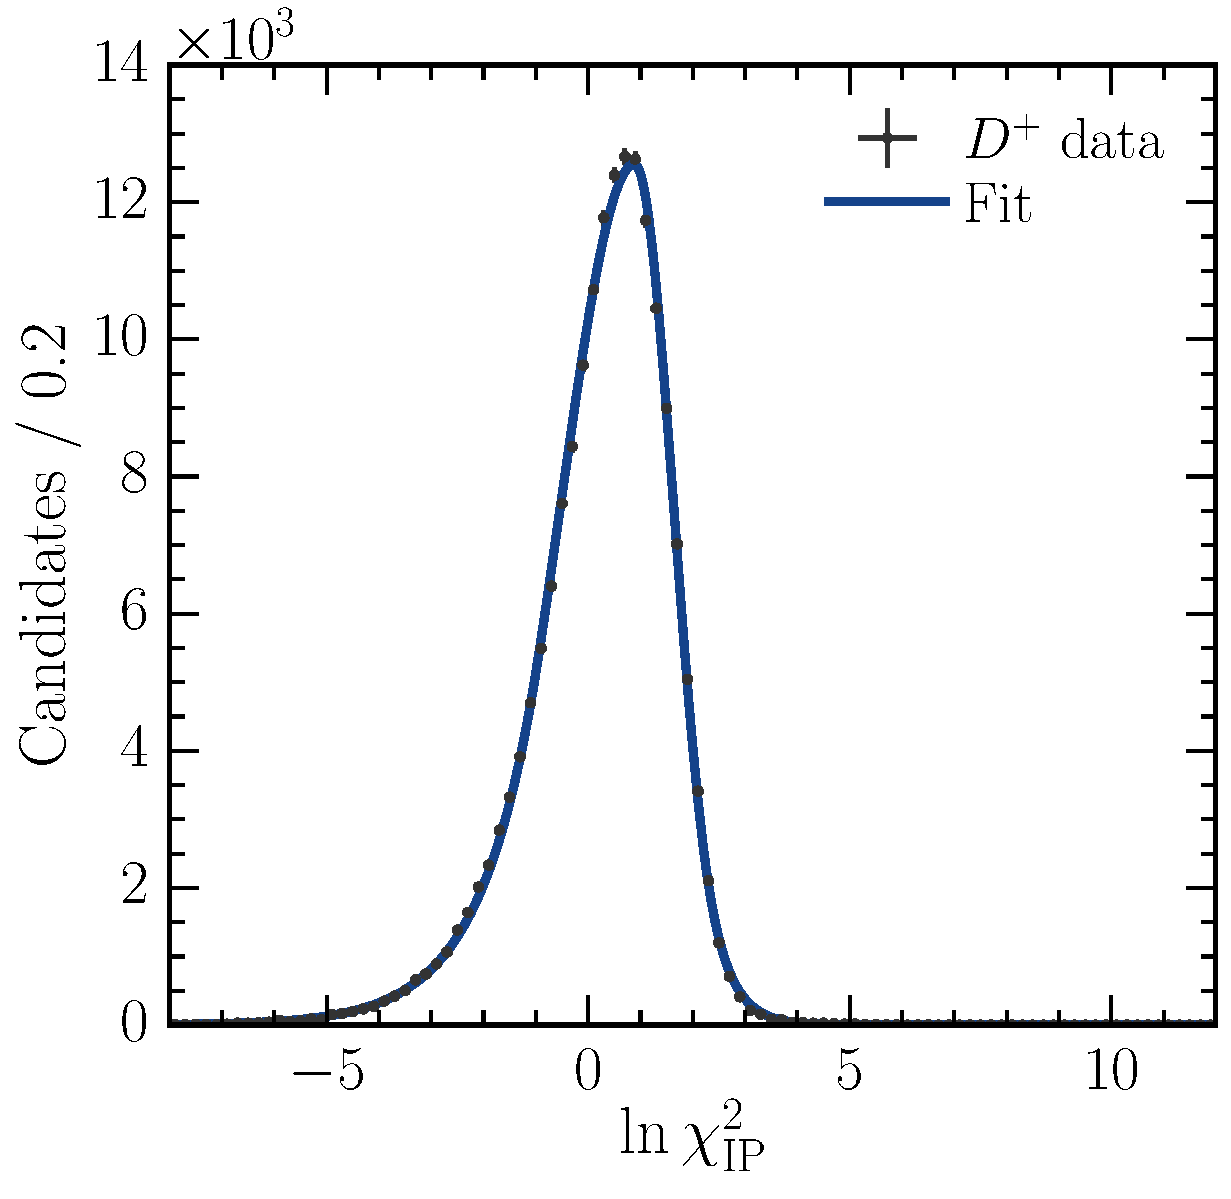
\includegraphics[width=\textwidth]{production/fitting/DpToKpipi_ipchisq_fit_pT_integrated_y_integrated_sig}
    \caption{Prompt}
    \label{fig:prod:fitting:prefits:DpToKpipi:prompt}
  \end{subfigure}
  \begin{subfigure}[b]{0.5\textwidth}
    \centering
    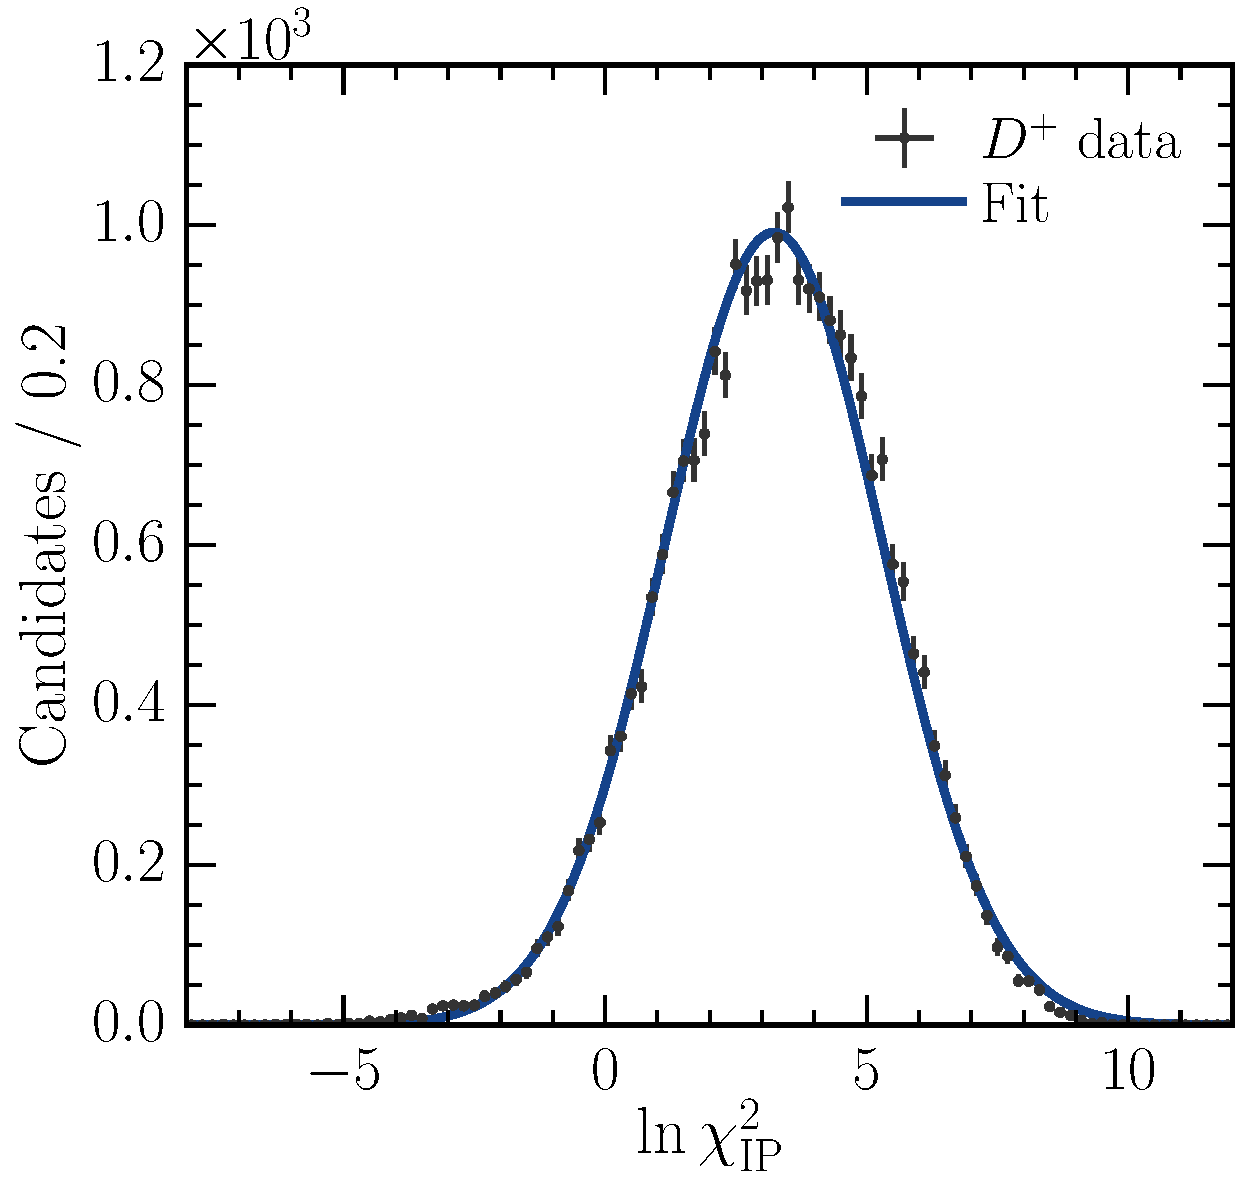
\includegraphics[width=\textwidth]{production/fitting/DpToKpipi_ipchisq_fit_pT_integrated_y_integrated_sec}
    \caption{Secondary}
    \label{fig:prod:fitting:prefits:DpToKpipi:secondary}
  \end{subfigure}
  \caption{%
    Distributions of \lnipchisq\ for simulated \DpToKpipi\ decays: prompt 
    signal \PDplus (\subref*{fig:prod:fitting:prefits:DpToKpipi:prompt}) and 
    secondary signal \PDplus 
    (\subref*{fig:prod:fitting:prefits:DpToKpipi:secondary}).
    The sum of the simultaneous likelihood fits in each \pTy\ bin is overlaid.
  }
  \label{fig:prod:fitting:prefits:DpToKpipi}
\end{figure}

\begin{figure}
  \begin{subfigure}[b]{0.5\textwidth}
    \centering
    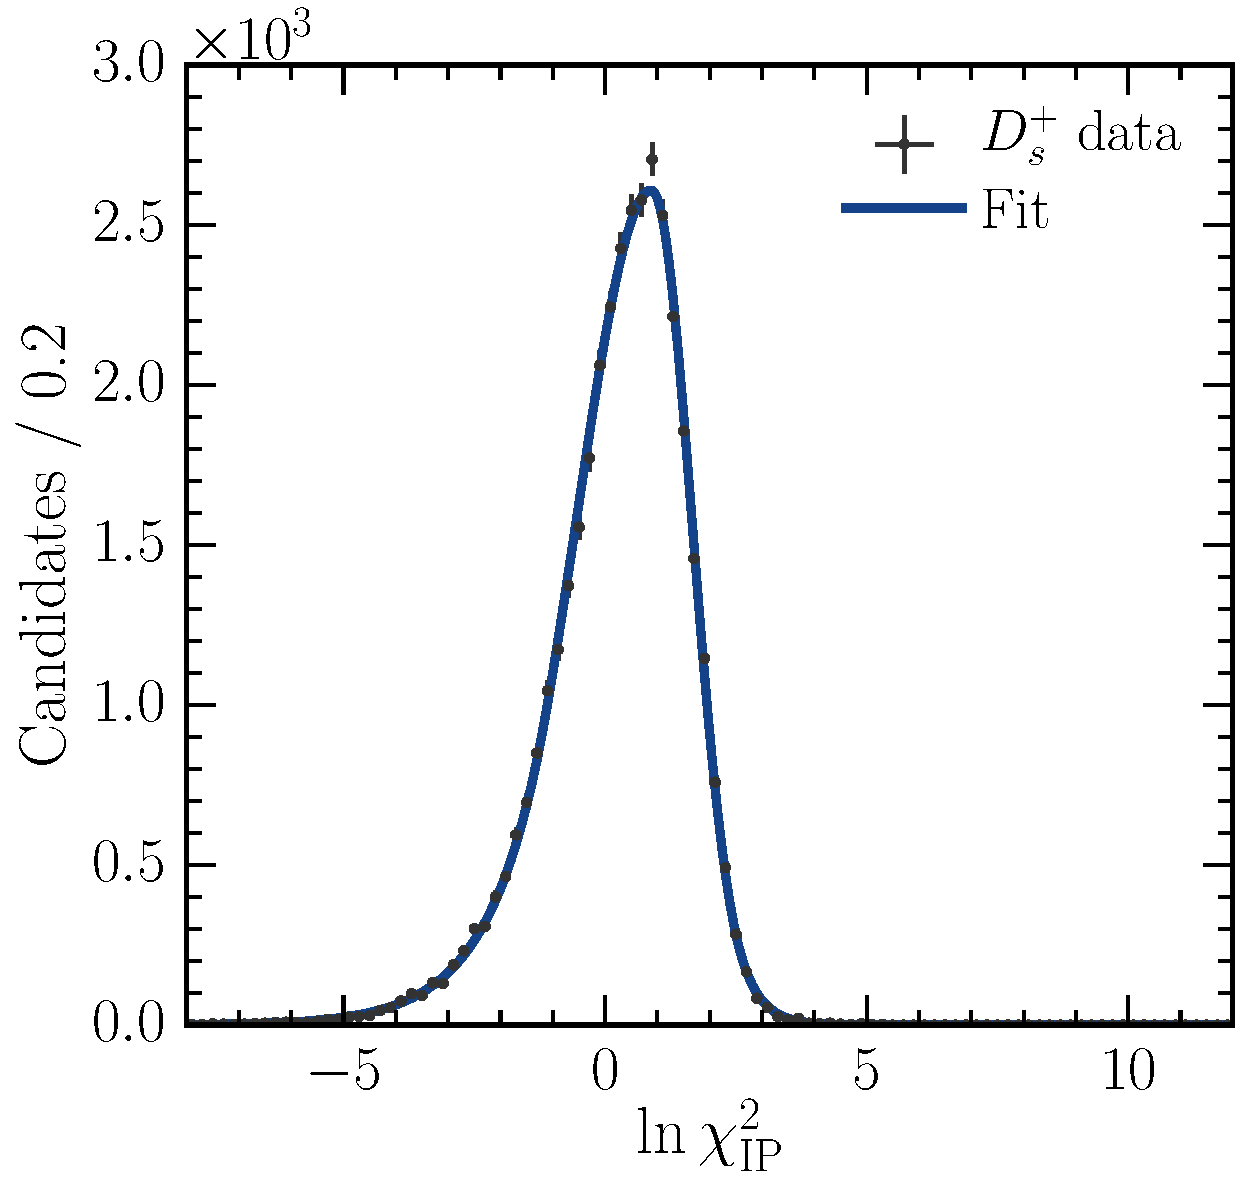
\includegraphics[width=\textwidth]{production/fitting/DsToKKpi_ipchisq_fit_pT_integrated_y_integrated_sig}
    \caption{Prompt}
    \label{fig:prod:fitting:prefits:DsToKKpi:prompt}
  \end{subfigure}
  \begin{subfigure}[b]{0.5\textwidth}
    \centering
    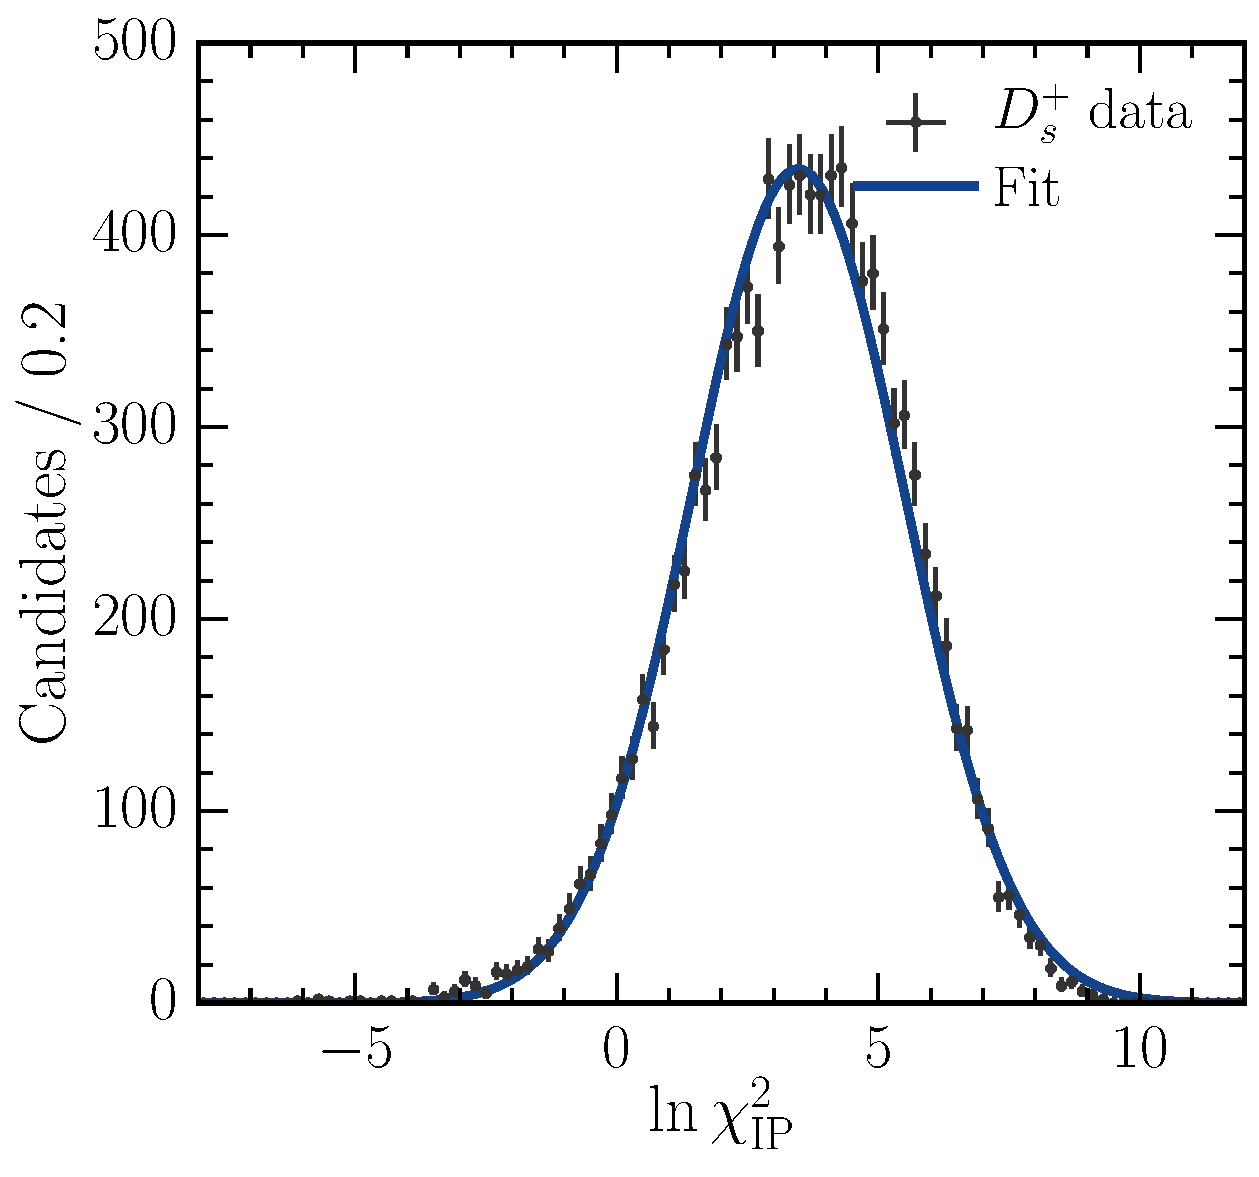
\includegraphics[width=\textwidth]{production/fitting/DsToKKpi_ipchisq_fit_pT_integrated_y_integrated_sec}
    \caption{Secondary}
    \label{fig:prod:fitting:prefits:DsToKKpi:secondary}
  \end{subfigure}
  \caption{%
    Distributions of \lnipchisq\ for simulated \DspTophipi\ decays: prompt 
    signal \PDsplus (\subref*{fig:prod:fitting:prefits:DsToKKpi:prompt}) and 
    secondary signal \PDsplus 
    (\subref*{fig:prod:fitting:prefits:DsToKKpi:secondary}).
    The sum of the simultaneous likelihood fits in each \pTy\ bin is overlaid.
  }
  \label{fig:prod:fitting:prefits:DsToKKpi}
\end{figure}

\begin{figure}
  \begin{subfigure}[b]{0.5\textwidth}
    \centering
    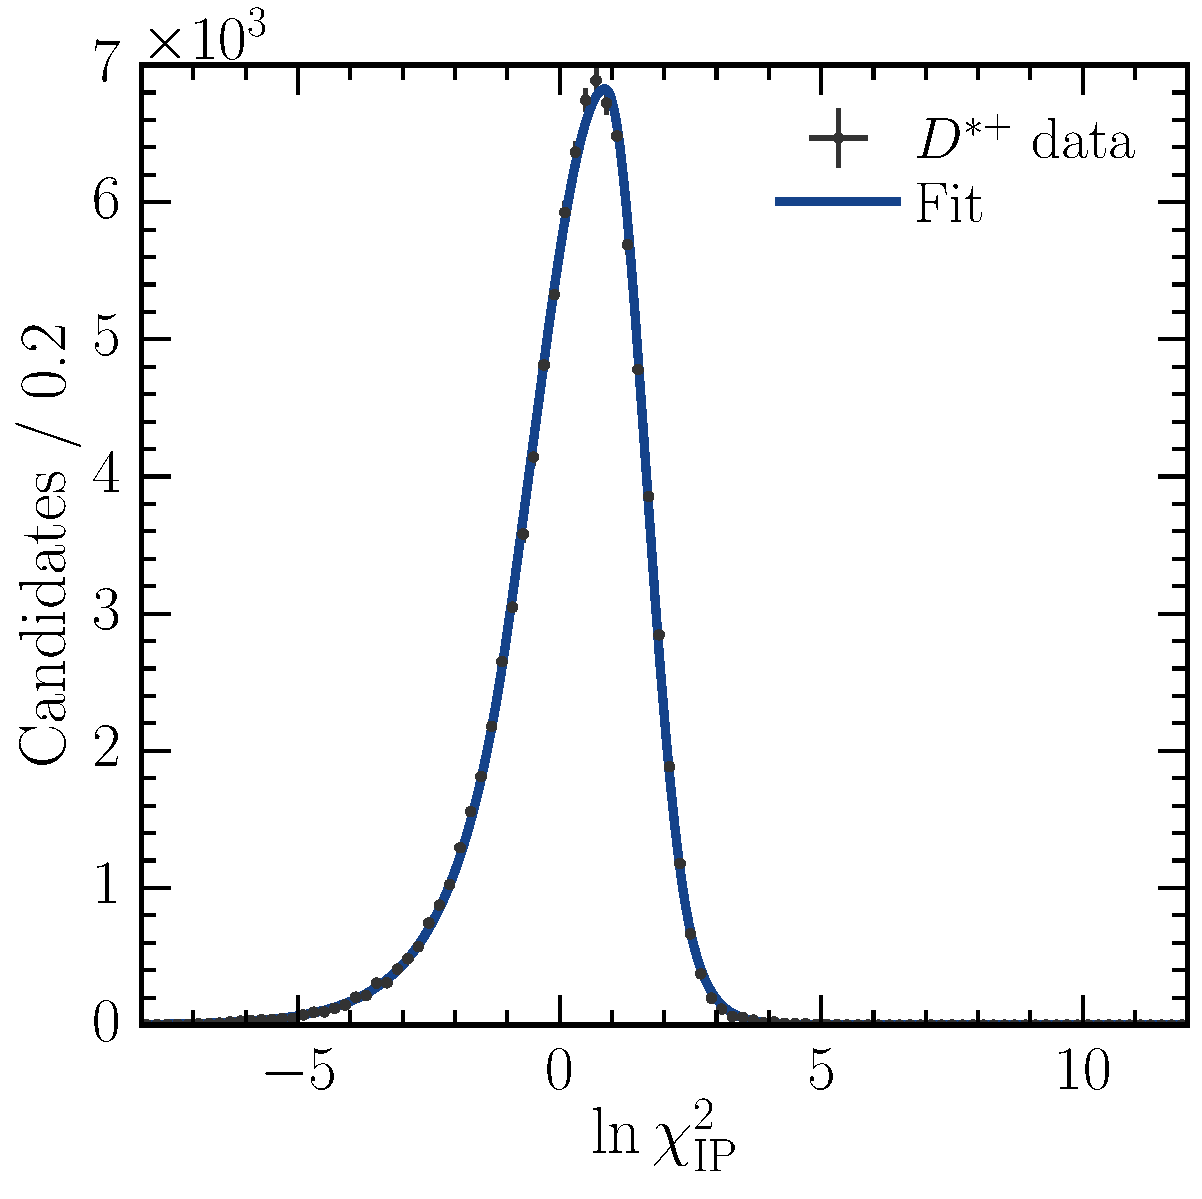
\includegraphics[width=\textwidth]{production/fitting/DstToD0pi_D0ToKpi_ipchisq_fit_pT_integrated_y_integrated_sig}
    \caption{Prompt}
    \label{fig:prod:fitting:prefits:DstToD0pi_D0ToKpi:prompt}
  \end{subfigure}
  \begin{subfigure}[b]{0.5\textwidth}
    \centering
    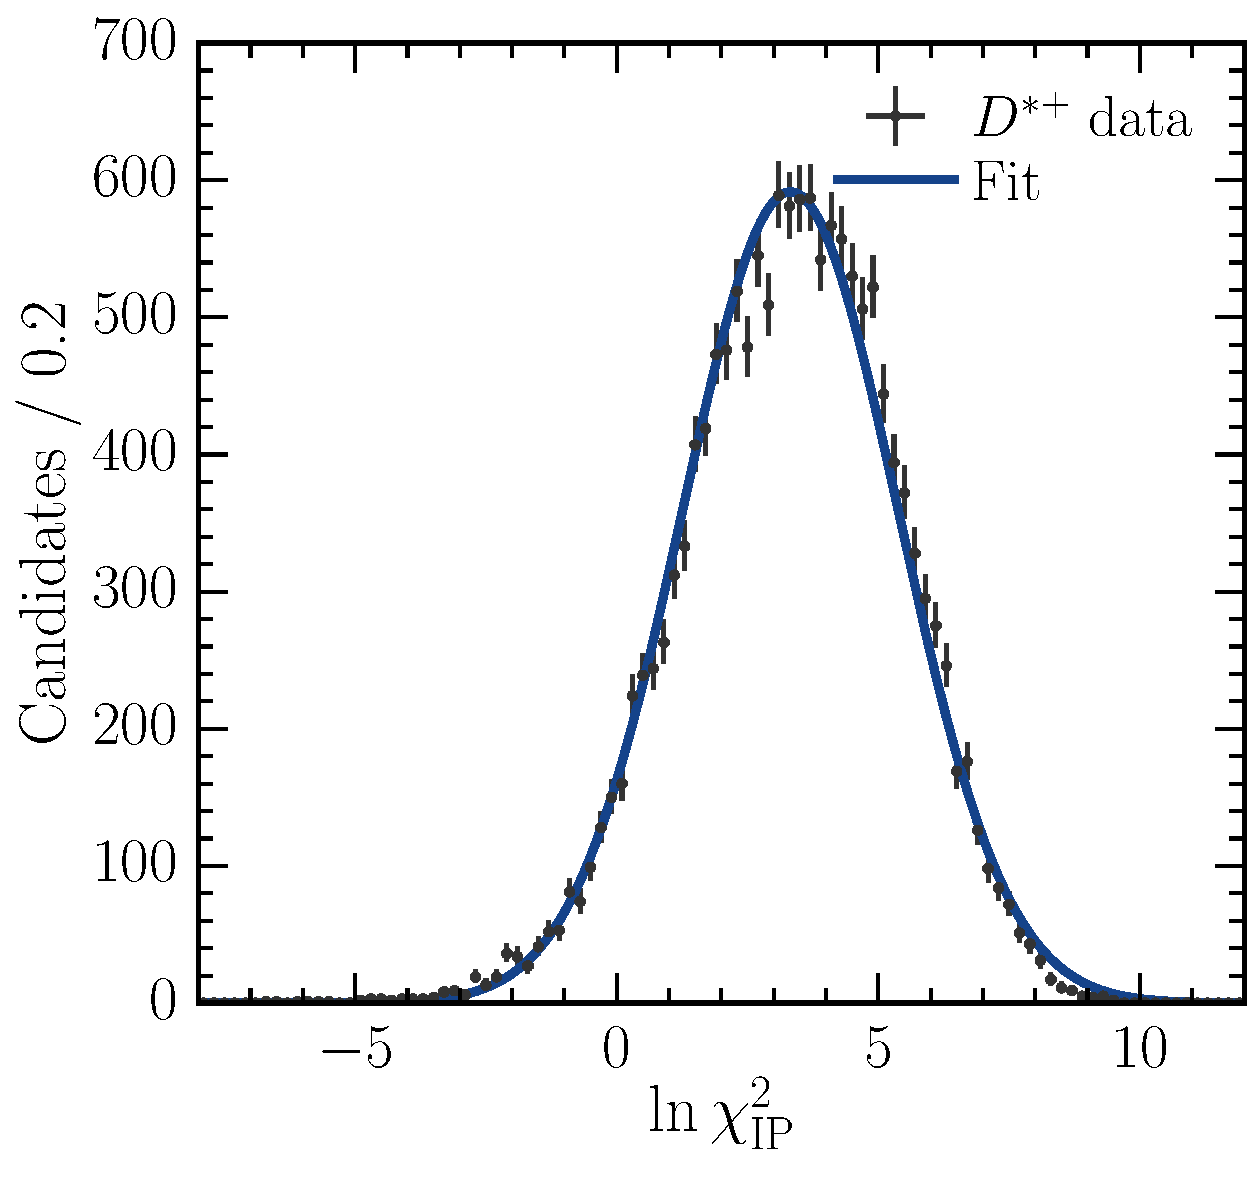
\includegraphics[width=\textwidth]{production/fitting/DstToD0pi_D0ToKpi_ipchisq_fit_pT_integrated_y_integrated_sec}
    \caption{Secondary}
    \label{fig:prod:fitting:prefits:DstToD0pi_D0ToKpi:secondary}
  \end{subfigure}
  \caption{%
    Distributions of \PDzero \lnipchisq\ for simulated \DstToDzpi, with 
    \DzToKpi, decays: prompt signal \PDstarp\
    (\subref*{fig:prod:fitting:prefits:DstToD0pi_D0ToKpi:prompt}) and secondary 
    signal \PDstarp\
    (\subref*{fig:prod:fitting:prefits:DstToD0pi_D0ToKpi:secondary}).
    The sum of the simultaneous likelihood fits in each \pTy\ bin is overlaid.
  }
  \label{fig:prod:fitting:prefits:DstToD0pi_D0ToKpi}
\end{figure}

\begin{figure}
  \begin{subfigure}[b]{0.5\textwidth}
    \centering
    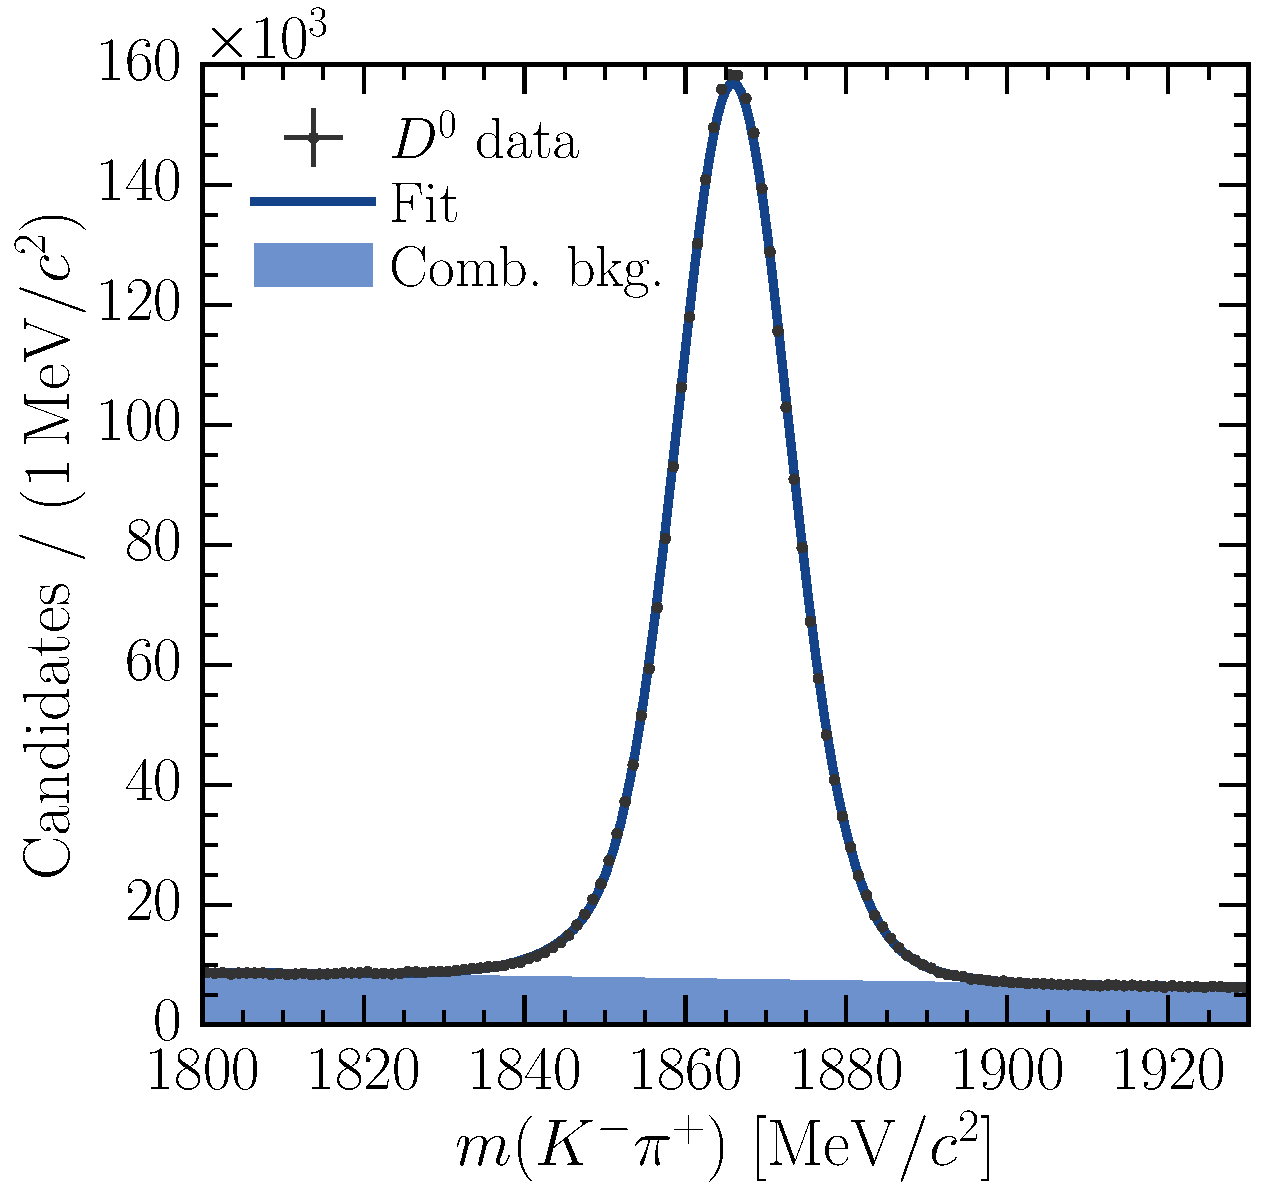
\includegraphics[width=\textwidth]{production/fitting/D0ToKpi_mass_fit_pT_integrated_y_integrated}
    \caption{Mass}
    \label{fig:prod:fitting:D0ToKpi:mass}
  \end{subfigure}
  \begin{subfigure}[b]{0.5\textwidth}
    \centering
    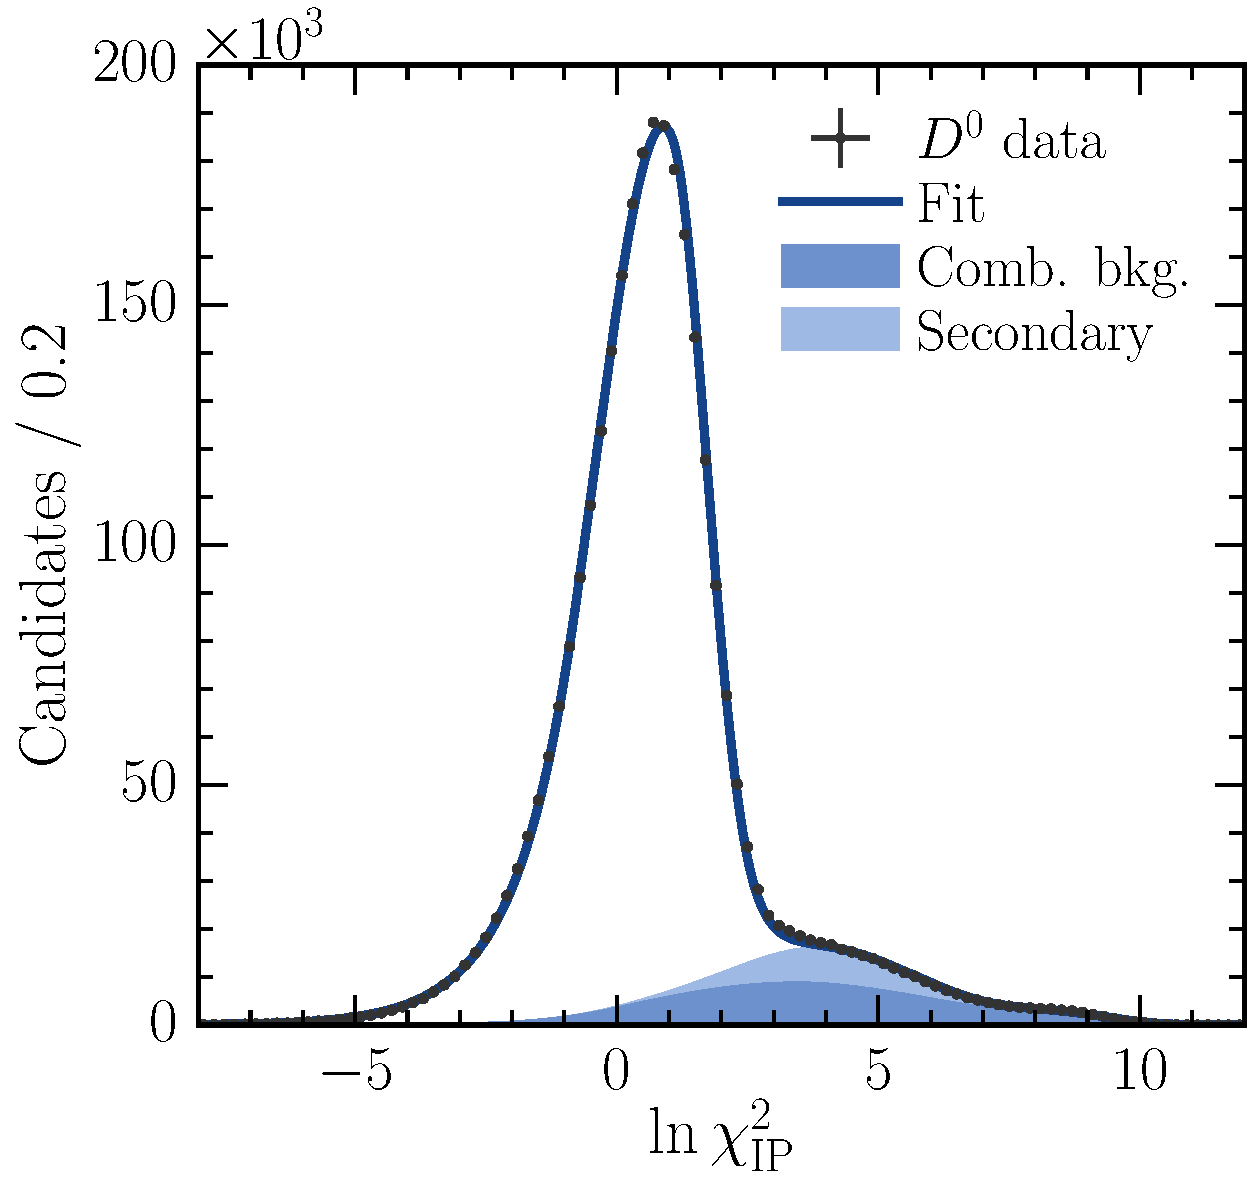
\includegraphics[width=\textwidth]{production/fitting/D0ToKpi_ipchisq_fit_pT_integrated_y_integrated}
    \caption{\lnipchisq}
    \label{fig:prod:fitting:D0ToKpi:ipchisq}
  \end{subfigure}
  \caption{%
    Distributions for fully selected \DzToKpi\ candidates: \PDzero\ invariant 
    mass (\subref*{fig:prod:fitting:D0ToKpi:mass}); and \PDzero\ \lnipchisq\ 
    (\subref*{fig:prod:fitting:D0ToKpi:ipchisq}) for a mass window of 
    $\pm\SI{20}{\MeVcc}$ around the nominal \PDzero mass.
    The sum of the simultaneous likelihood fits in each \pTy\ bin is shown, 
    with components as indicated in the legends.
  }
  \label{fig:prod:fitting:D0ToKpi}
\end{figure}

\begin{figure}
  \begin{subfigure}[b]{0.5\textwidth}
    \centering
    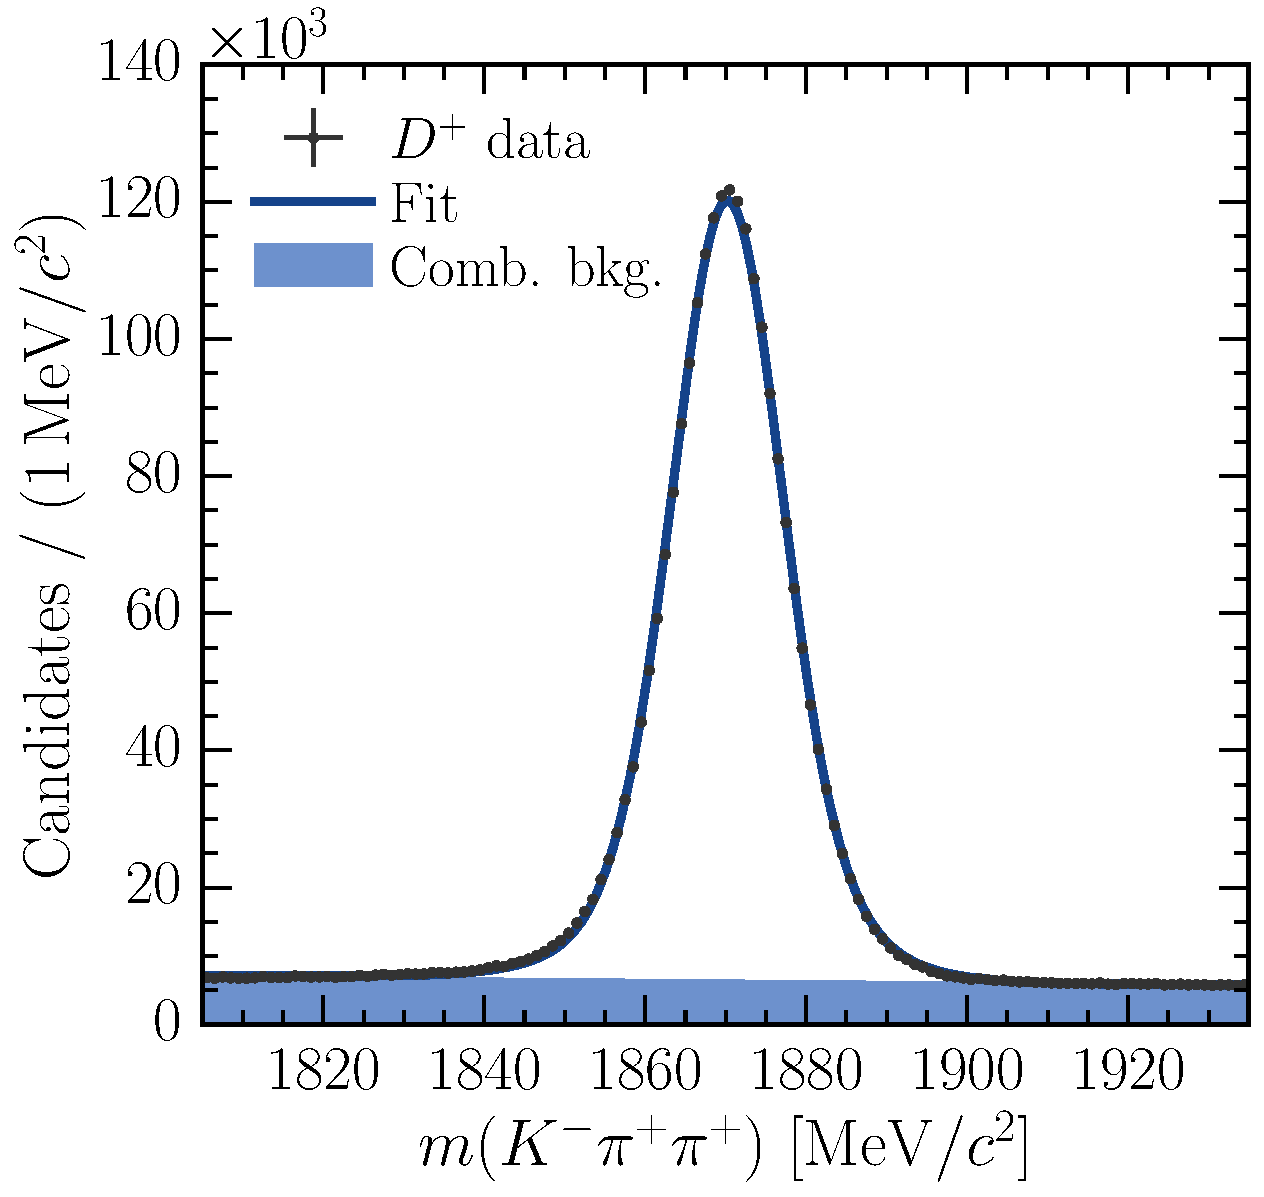
\includegraphics[width=\textwidth]{production/fitting/DpToKpipi_mass_fit_pT_integrated_y_integrated}
    \caption{Mass}
    \label{fig:prod:fitting:DpToKpipi:mass}
  \end{subfigure}
  \begin{subfigure}[b]{0.5\textwidth}
    \centering
    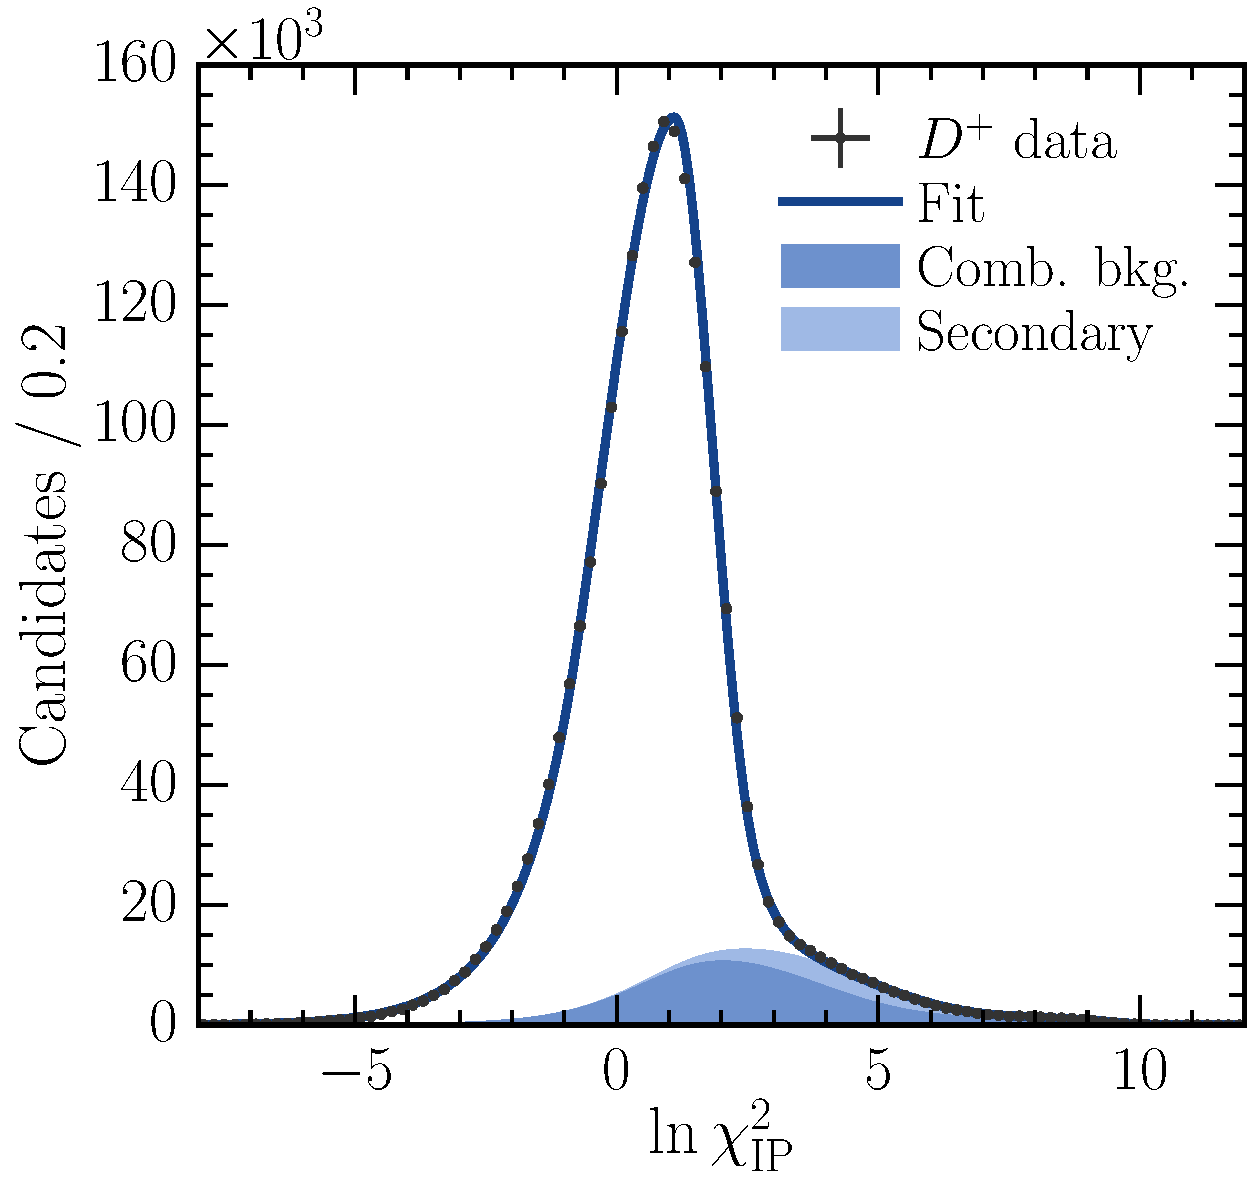
\includegraphics[width=\textwidth]{production/fitting/DpToKpipi_ipchisq_fit_pT_integrated_y_integrated}
    \caption{\lnipchisq}
    \label{fig:prod:fitting:DpToKpipi:ipchisq}
  \end{subfigure}
  \caption{%
    Distributions for fully selected \DpToKpipi\ candidates: \PDplus\ invariant 
    mass (\subref*{fig:prod:fitting:DpToKpipi:mass}); and \PDplus\ \lnipchisq\ 
    (\subref*{fig:prod:fitting:DpToKpipi:ipchisq}) for a mass window of 
    $\pm\SI{20}{\MeVcc}$ around the nominal \PDplus mass.
    The sum of the simultaneous likelihood fits in each \pTy\ bin is shown, 
    with components as indicated in the legends.
  }
  \label{fig:prod:fitting:DpToKpipi}
\end{figure}

\begin{figure}
  \begin{subfigure}[b]{0.5\textwidth}
    \centering
    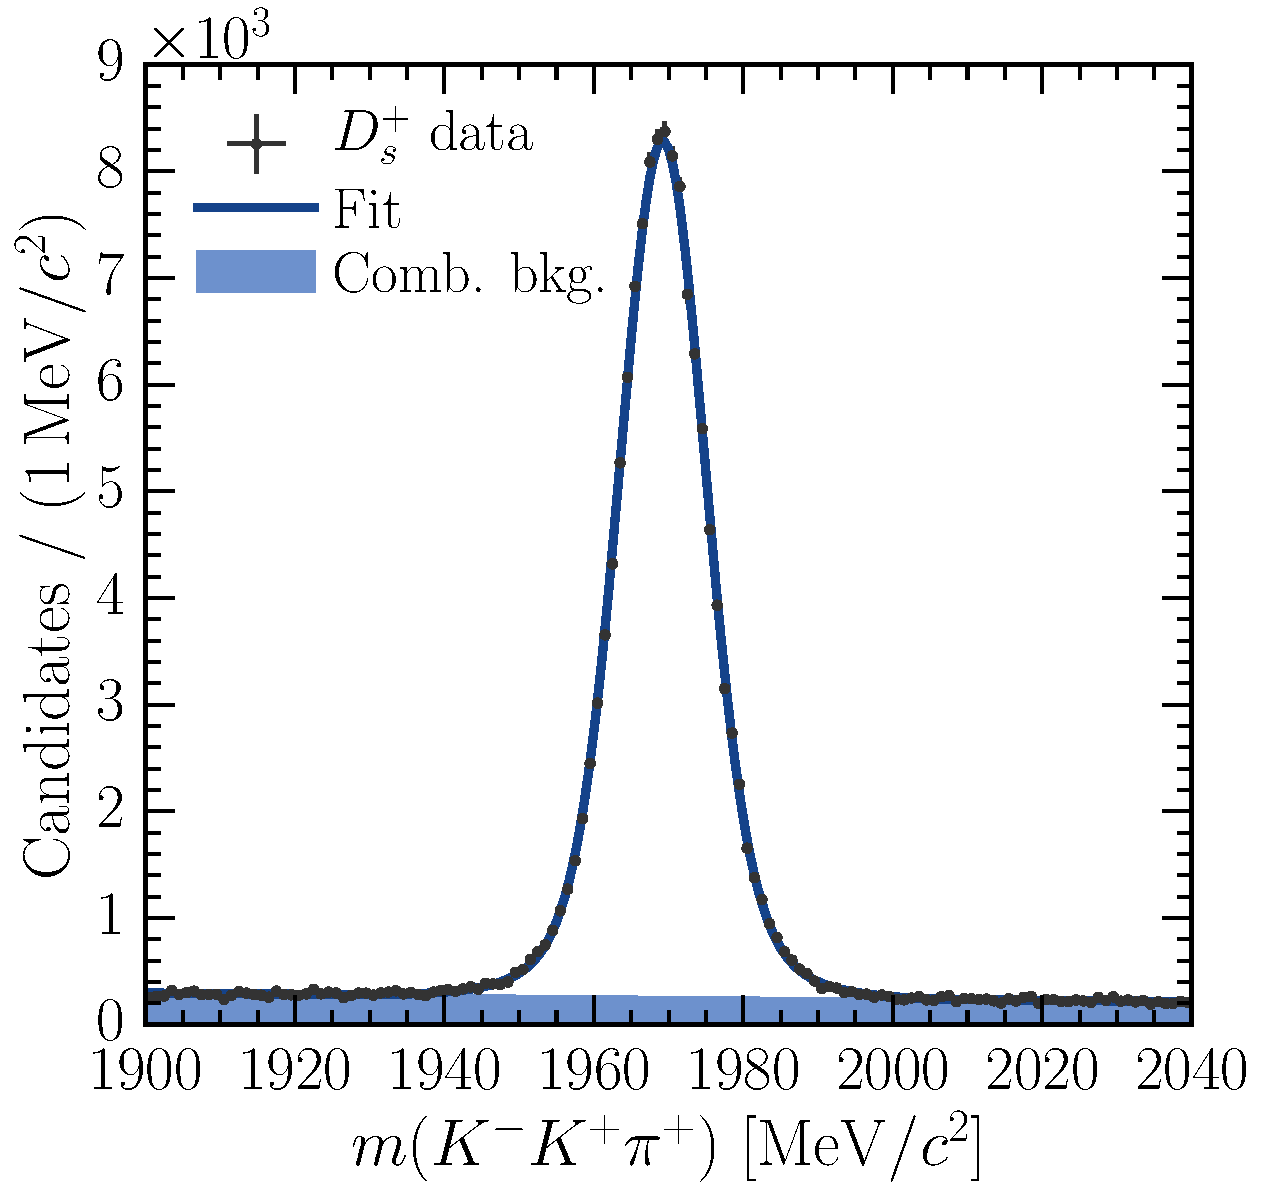
\includegraphics[width=\textwidth]{production/fitting/DsToKKpi_mass_fit_pT_integrated_y_integrated}
    \caption{Mass}
    \label{fig:prod:fitting:DsToKKpi:mass}
  \end{subfigure}
  \begin{subfigure}[b]{0.5\textwidth}
    \centering
    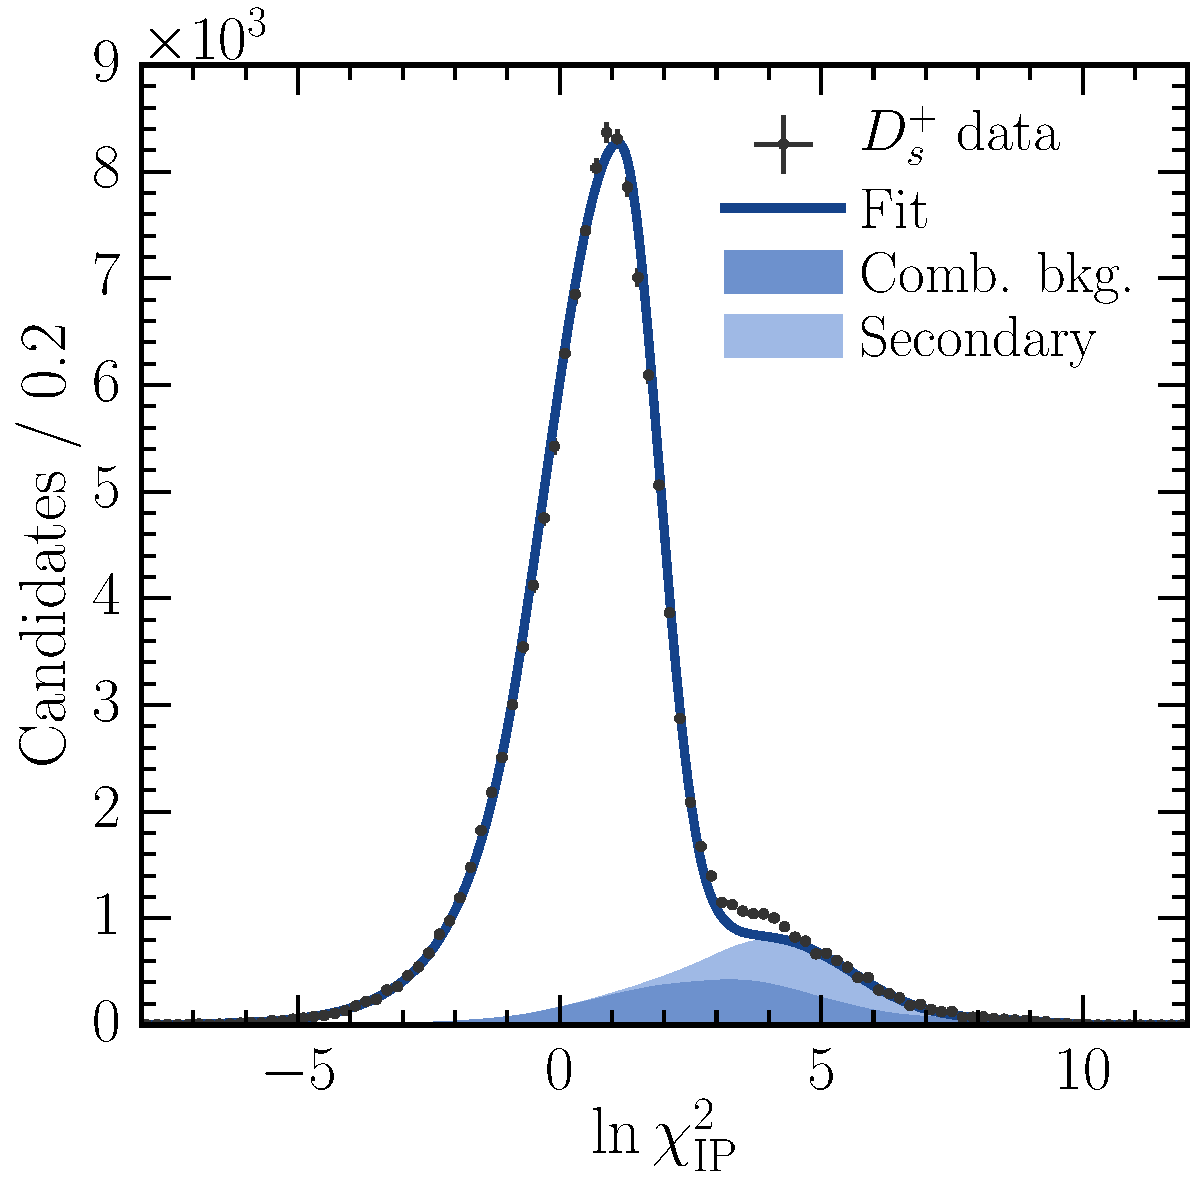
\includegraphics[width=\textwidth]{production/fitting/DsToKKpi_ipchisq_fit_pT_integrated_y_integrated}
    \caption{\lnipchisq}
    \label{fig:prod:fitting:DsToKKpi:ipchisq}
  \end{subfigure}
  \caption{%
    Distributions for fully selected \DspTophipi\ candidates: \PDsplus\ 
    invariant mass (\subref*{fig:prod:fitting:DpToKpipi:mass}); and \PDsplus\ 
    \lnipchisq\ (\subref*{fig:prod:fitting:DpToKpipi:ipchisq}) for a mass 
    window of $\pm\SI{20}{\MeVcc}$ around the nominal \PDsplus mass.
    The sum of the simultaneous likelihood fits in each \pTy\ bin is shown, 
    with components as indicated in the legends.
  }
  \label{fig:prod:fitting:DsToKKpi}
\end{figure}

\begin{figure}
  \begin{subfigure}[b]{0.5\textwidth}
    \centering
    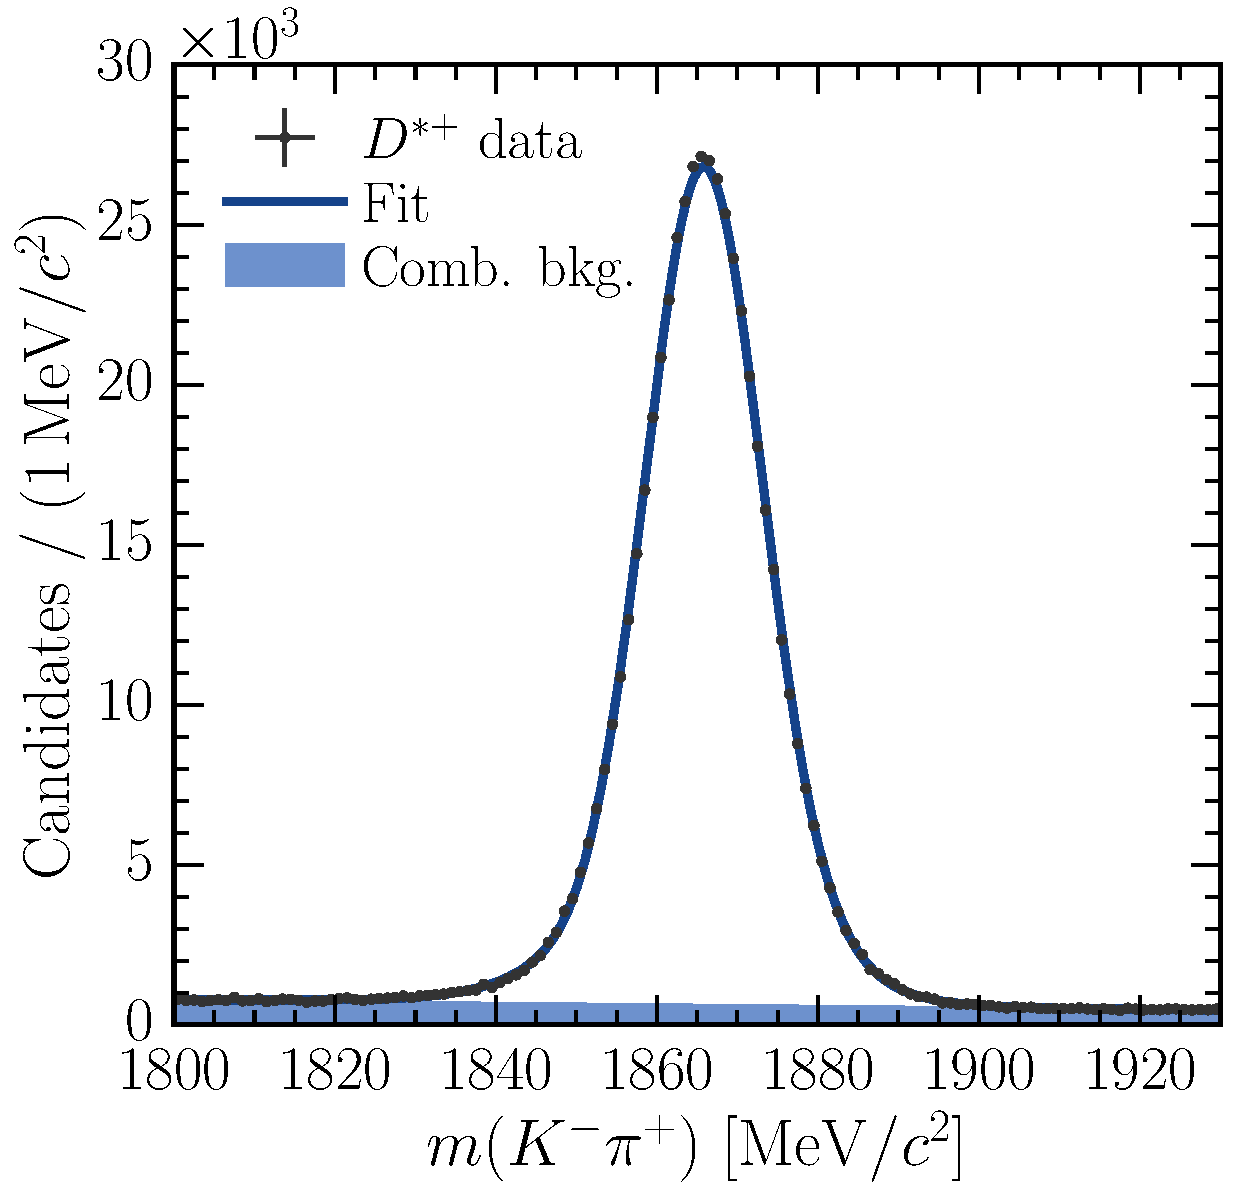
\includegraphics[width=\textwidth]{production/fitting/DstToD0pi_D0ToKpi_mass_fit_pT_integrated_y_integrated}
    \caption{\PDzero mass}
    \label{fig:prod:fitting:DstToD0pi_D0ToKpi:mass}
  \end{subfigure}
  \begin{subfigure}[b]{0.5\textwidth}
    \centering
    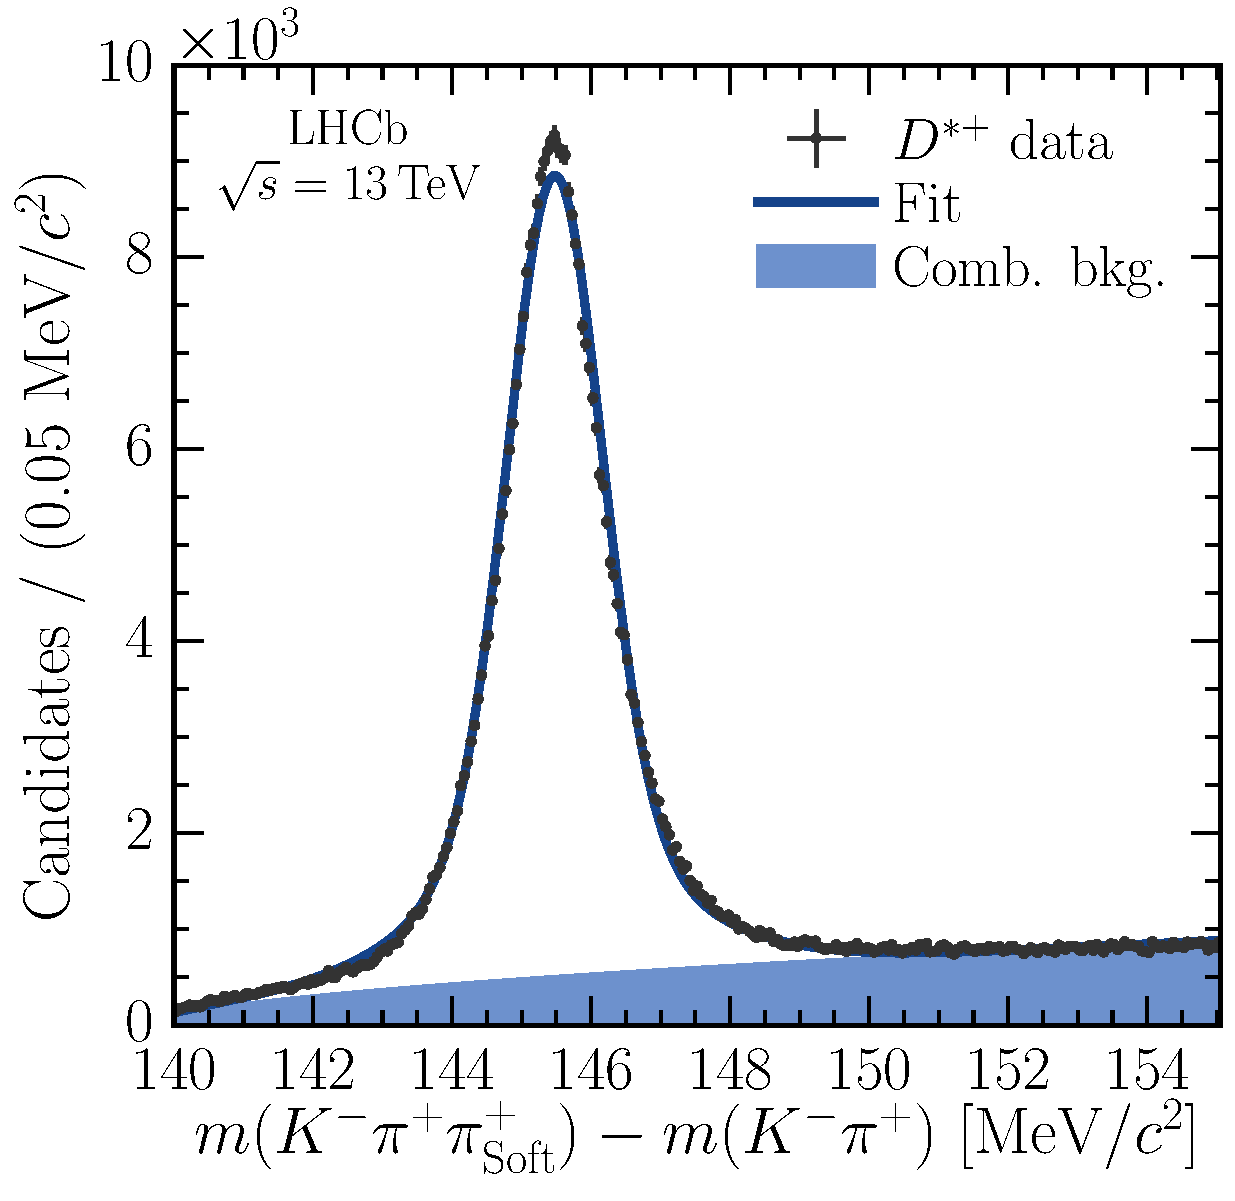
\includegraphics[width=\textwidth]{production/fitting/DstToD0pi_D0ToKpi_delta_mass_fit_pT_integrated_y_integrated}
    \caption{Delta mass}
    \label{fig:prod:fitting:DstToD0pi_D0ToKpi:delta_mass}
  \end{subfigure}
  \begin{subfigure}[b]{0.5\textwidth}
    \centering
    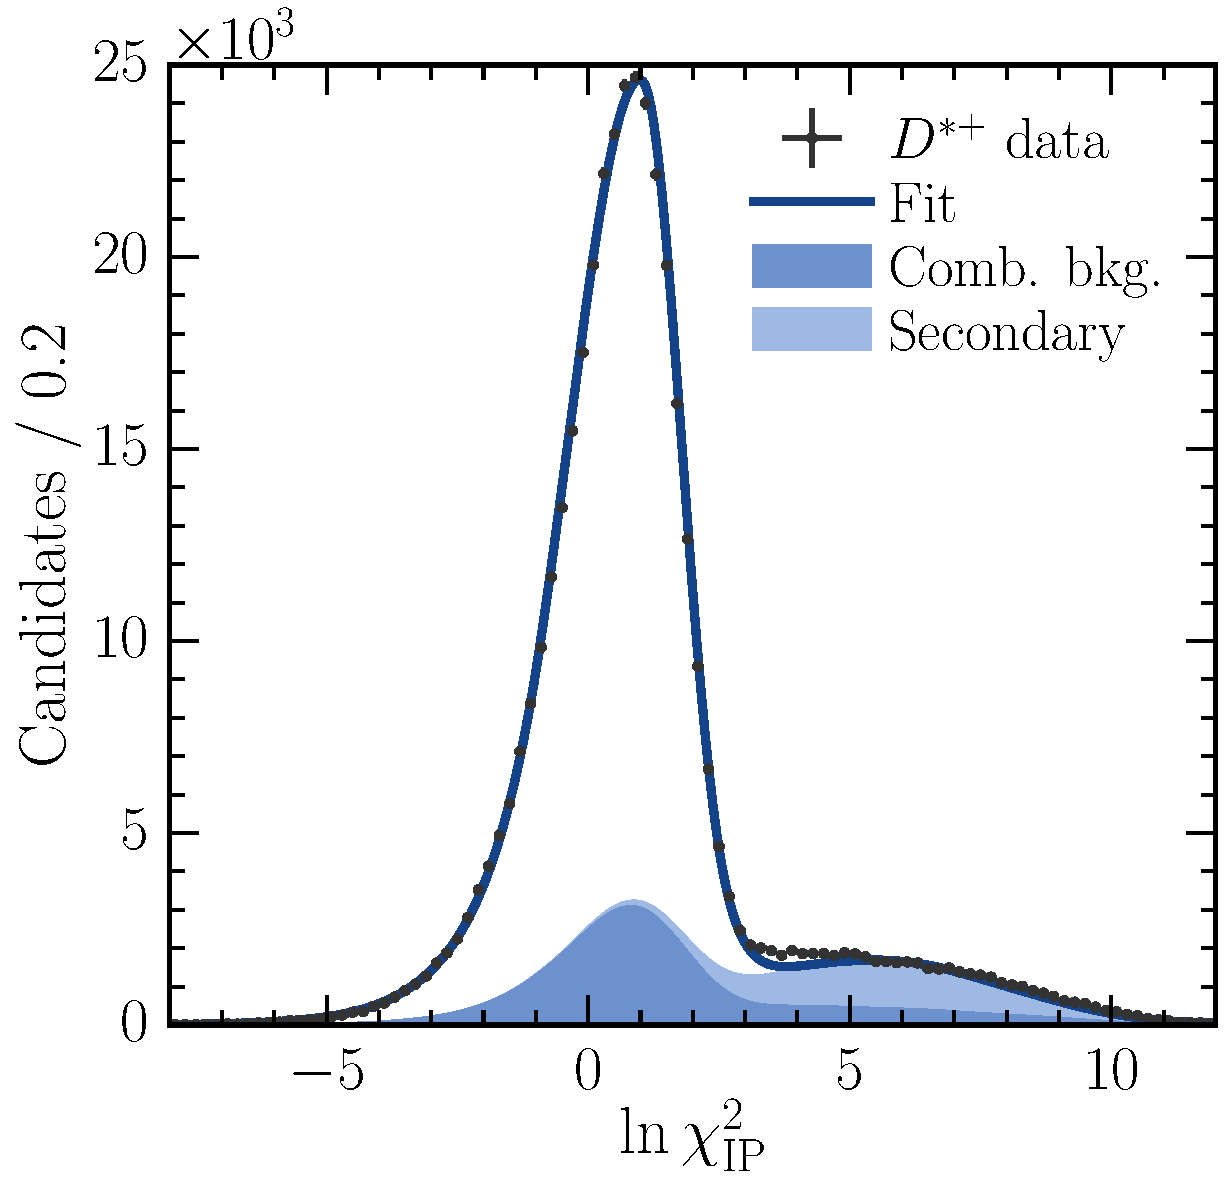
\includegraphics[width=\textwidth]{production/fitting/DstToD0pi_D0ToKpi_ipchisq_fit_pT_integrated_y_integrated}
    \caption{\lnipchisq}
    \label{fig:prod:fitting:DstToD0pi_D0ToKpi:ipchisq}
  \end{subfigure}
  \caption{%
    Distributions for fully selected \PDstarp\ candidates, with \DzToKpi: 
    \PDzero\ invariant mass 
    (\subref*{fig:prod:fitting:DstToD0pi_D0ToKpi:mass}); $\deltam = m(\PDstarp) 
    - m(\PDzero)$ (\subref*{fig:prod:fitting:DstToD0pi_D0ToKpi:delta_mass}) for 
    a mass window of $\pm\SI{20}{\MeVcc}$ around the nominal \PDzero mass; and 
    \PDzero\ \lnipchisq\ (\subref*{fig:prod:fitting:DstToD0pi_D0ToKpi:ipchisq}) 
    with an additional mass window of $\pm\SI{3}{\MeVcc}$ around the nominal 
    \PDstarp-\PDzero\ mass difference.
    The sum of the simultaneous likelihood fits in each \pTy\ bin is shown, 
    with components as indicated in the legends.
  }
  \label{fig:prod:fitting:DstToD0pi_D0ToKpi}
\end{figure}

% TODO empty cells don't have a dash in anymore. that's OK as long as the
% caption is updated (and that it's consistent with the presentation in the
% other tables).
\begin{sidewaystable}
  \caption{%
    Prompt signal yields for \DzToKpi\ measured in \PDzero \pTy\ bins.
    Cells marked with a dash `-' indicate bins where insufficient data were 
    available for a statistically significant prompt signal yield measurement.
  }
  \label{tab:prod:fitting:D0ToKpi}
  \centering
  \renewcommand{\arraystretch}{1.0}
\begin{tabular}{lr@{\hskip+0.2em}c@{\hskip+0.2em}r@{\hskip+0.2em}c@{\hskip+0.2em}rr@{\hskip+0.2em}c@{\hskip+0.2em}r@{\hskip+0.2em}c@{\hskip+0.2em}rr@{\hskip+0.2em}c@{\hskip+0.2em}r@{\hskip+0.2em}c@{\hskip+0.2em}rr@{\hskip+0.2em}c@{\hskip+0.2em}r@{\hskip+0.2em}c@{\hskip+0.2em}rr@{\hskip+0.2em}c@{\hskip+0.2em}r@{\hskip+0.2em}c@{\hskip+0.2em}r}
\toprule&\multicolumn{25}{c}{$y$}\\
$p_{\text{T}} [\text{MeV}/c]$ & \multicolumn{5}{c}{$[2,2.5]$} & \multicolumn{5}{c}{$[2.5,3]$} & \multicolumn{5}{c}{$[3,3.5]$} & \multicolumn{5}{c}{$[3.5,4]$} & \multicolumn{5}{c}{$[4,4.5]$} \\
\midrule$[14000,15000]$ & \multicolumn{5}{c}{$550 \pm 30$} & \multicolumn{5}{c}{$610 \pm 30$} & \multicolumn{5}{c}{$72 \pm 9$} & \multicolumn{5}{c}{ } & \multicolumn{5}{c}{ } \\
$[13000,14000]$ & \multicolumn{5}{c}{$860 \pm 30$} & \multicolumn{5}{c}{$970 \pm 40$} & \multicolumn{5}{c}{$180 \pm 20$} & \multicolumn{5}{c}{ } & \multicolumn{5}{c}{ } \\
$[12000,13000]$ & \multicolumn{5}{c}{$1250 \pm 40$} & \multicolumn{5}{c}{$1580 \pm 40$} & \multicolumn{5}{c}{$420 \pm 30$} & \multicolumn{5}{c}{ } & \multicolumn{5}{c}{ } \\
$[11000,12000]$ & \multicolumn{5}{c}{$1910 \pm 50$} & \multicolumn{5}{c}{$2520 \pm 50$} & \multicolumn{5}{c}{$890 \pm 30$} & \multicolumn{5}{c}{ } & \multicolumn{5}{c}{ } \\
$[10000,11000]$ & \multicolumn{5}{c}{$2990 \pm 60$} & \multicolumn{5}{c}{$3890 \pm 70$} & \multicolumn{5}{c}{$1880 \pm 50$} & \multicolumn{5}{c}{$32 \pm 6$} & \multicolumn{5}{c}{ } \\
$[9000,10000]$ & \multicolumn{5}{c}{$4830 \pm 70$} & \multicolumn{5}{c}{$6420 \pm 80$} & \multicolumn{5}{c}{$3810 \pm 70$} & \multicolumn{5}{c}{$170 \pm 20$} & \multicolumn{5}{c}{ } \\
$[8000,9000]$ & \multicolumn{5}{c}{$7570 \pm 90$} & \multicolumn{5}{c}{$10900 \pm 200$} & \multicolumn{5}{c}{$7250 \pm 90$} & \multicolumn{5}{c}{$680 \pm 30$} & \multicolumn{5}{c}{ } \\
$[7000,8000]$ & \multicolumn{5}{c}{$12000 \pm 200$} & \multicolumn{5}{c}{$18600 \pm 200$} & \multicolumn{5}{c}{$13700 \pm 200$} & \multicolumn{5}{c}{$2460 \pm 50$} & \multicolumn{5}{c}{ } \\
$[6000,7000]$ & \multicolumn{5}{c}{$19100 \pm 200$} & \multicolumn{5}{c}{$32400 \pm 200$} & \multicolumn{5}{c}{$25500 \pm 200$} & \multicolumn{5}{c}{$7510 \pm 90$} & \multicolumn{5}{c}{$39 \pm 6$} \\
$[5000,6000]$ & \multicolumn{5}{c}{$30100 \pm 200$} & \multicolumn{5}{c}{$56300 \pm 300$} & \multicolumn{5}{c}{$47000 \pm 300$} & \multicolumn{5}{c}{$19000 \pm 200$} & \multicolumn{5}{c}{$670 \pm 30$} \\
$[4000,5000]$ & \multicolumn{5}{c}{$44800 \pm 300$} & \multicolumn{5}{c}{$98500 \pm 400$} & \multicolumn{5}{c}{$85500 \pm 300$} & \multicolumn{5}{c}{$41900 \pm 300$} & \multicolumn{5}{c}{$3990 \pm 70$} \\
$[3500,4000]$ & \multicolumn{5}{c}{$28000 \pm 200$} & \multicolumn{5}{c}{$70900 \pm 300$} & \multicolumn{5}{c}{$63600 \pm 300$} & \multicolumn{5}{c}{$34100 \pm 200$} & \multicolumn{5}{c}{$5290 \pm 80$} \\
$[3000,3500]$ & \multicolumn{5}{c}{$30600 \pm 200$} & \multicolumn{5}{c}{$85600 \pm 300$} & \multicolumn{5}{c}{$80500 \pm 300$} & \multicolumn{5}{c}{$44400 \pm 300$} & \multicolumn{5}{c}{$8560 \pm 100$} \\
$[2500,3000]$ & \multicolumn{5}{c}{$31700 \pm 200$} & \multicolumn{5}{c}{$98100 \pm 400$} & \multicolumn{5}{c}{$97000 \pm 400$} & \multicolumn{5}{c}{$54400 \pm 300$} & \multicolumn{5}{c}{$11800 \pm 200$} \\
$[2000,2500]$ & \multicolumn{5}{c}{$30100 \pm 200$} & \multicolumn{5}{c}{$102200 \pm 400$} & \multicolumn{5}{c}{$106700 \pm 400$} & \multicolumn{5}{c}{$62200 \pm 300$} & \multicolumn{5}{c}{$14400 \pm 200$} \\
$[1500,2000]$ & \multicolumn{5}{c}{$27500 \pm 200$} & \multicolumn{5}{c}{$96600 \pm 400$} & \multicolumn{5}{c}{$107700 \pm 400$} & \multicolumn{5}{c}{$64400 \pm 300$} & \multicolumn{5}{c}{$15300 \pm 200$} \\
$[1000,1500]$ & \multicolumn{5}{c}{$22100 \pm 200$} & \multicolumn{5}{c}{$84900 \pm 300$} & \multicolumn{5}{c}{$99900 \pm 400$} & \multicolumn{5}{c}{$60700 \pm 300$} & \multicolumn{5}{c}{$14900 \pm 200$} \\
$[0,1000]$ & \multicolumn{5}{c}{$20300 \pm 200$} & \multicolumn{5}{c}{$85900 \pm 300$} & \multicolumn{5}{c}{$108800 \pm 400$} & \multicolumn{5}{c}{$69400 \pm 300$} & \multicolumn{5}{c}{$17200 \pm 200$} \\
\bottomrule\end{tabular}

\end{sidewaystable}

\begin{sidewaystable}
  \caption{%
    Prompt signal yields for \DpToKpipi\ measured in \PDplus \pTy\ bins.
    Cells marked with a dash `-' indicate bins where insufficient data were 
    available for a statistically significant prompt signal yield measurement.
  }
  \label{tab:prod:fitting:DpToKpipi}
  \centering
  \renewcommand{\arraystretch}{1.0}
\begin{tabular}{lccccc}
\toprule&\multicolumn{5}{c}{$y$}\\
$p_{\text{T}} [\text{MeV}/c]$ & $[2,2.5[$ & $[2.5,3[$ & $[3,3.5[$ & $[3.5,4[$ & $[4,4.5[$ \\
\midrule$[0,1000[$ & $20.8 \pm 1.8$ & $895.1 \pm 34.2$ & $2582.2 \pm 63.6$ & $2032.8 \pm 64.1$ & $457.8 \pm 30.2$ \\
$[1000,1500[$ & $632.1 \pm 23.9$ & $11274.3 \pm 117.7$ & $21812.8 \pm 171.3$ & $16199.2 \pm 156.2$ & $3822.3 \pm 76.7$ \\
$[1500,2000[$ & $3873.6 \pm 63.4$ & $39656.3 \pm 215.8$ & $62963.3 \pm 281.5$ & $44300.2 \pm 243.0$ & $10247.4 \pm 116.4$ \\
$[2000,2500[$ & $9884.4 \pm 100.9$ & $70631.5 \pm 282.8$ & $99062.7 \pm 343.7$ & $67130.2 \pm 287.0$ & $15744.4 \pm 139.2$ \\
$[2500,3000[$ & $14409.6 \pm 122.3$ & $83863.9 \pm 304.5$ & $107012.2 \pm 351.2$ & $70423.1 \pm 288.4$ & $17345.3 \pm 142.8$ \\
$[3000,3500[$ & $16796.2 \pm 131.8$ & $78838.1 \pm 293.5$ & $93292.9 \pm 324.5$ & $60555.9 \pm 263.8$ & $14807.9 \pm 130.1$ \\
$[3500,4000[$ & $16972.7 \pm 132.2$ & $68260.3 \pm 271.7$ & $76260.2 \pm 291.5$ & $48134.3 \pm 233.9$ & $11515.3 \pm 113.4$ \\
$[4000,5000[$ & $30571.0 \pm 178.1$ & $99186.0 \pm 328.1$ & $103817.4 \pm 340.4$ & $63395.0 \pm 267.1$ & $12705.9 \pm 118.6$ \\
$[5000,6000[$ & $22656.6 \pm 153.5$ & $61121.3 \pm 256.8$ & $59612.1 \pm 256.2$ & $33210.3 \pm 191.8$ & $4746.6 \pm 72.9$ \\
$[6000,7000[$ & $16151.9 \pm 129.4$ & $35998.3 \pm 197.2$ & $33704.5 \pm 191.5$ & $16377.2 \pm 133.3$ & $1260.6 \pm 35.8$ \\
$[7000,8000[$ & $10806.7 \pm 106.1$ & $22215.4 \pm 154.5$ & $19385.3 \pm 144.6$ & $7547.0 \pm 90.1$ & $260.6 \pm 14.2$ \\
$[8000,9000[$ & $7532.2 \pm 88.0$ & $13683.2 \pm 120.7$ & $11362.8 \pm 110.0$ & $3302.6 \pm 58.7$ & $40.9 \pm 3.3$ \\
$[9000,10000[$ & $5014.7 \pm 71.2$ & $8727.6 \pm 95.8$ & $6817.4 \pm 84.6$ & $1386.0 \pm 37.0$ & - \\
$[10000,11000[$ & $3361.3 \pm 58.0$ & $5446.1 \pm 75.1$ & $3908.4 \pm 63.5$ & $491.4 \pm 20.9$ & - \\
$[11000,12000[$ & $2376.2 \pm 48.4$ & $3565.6 \pm 60.5$ & $2325.9 \pm 48.1$ & $187.1 \pm 10.8$ & - \\
$[12000,13000[$ & $1600.2 \pm 38.7$ & $2377.4 \pm 48.6$ & $1283.0 \pm 35.2$ & $61.4 \pm 3.8$ & - \\
$[13000,14000[$ & $1114.2 \pm 31.8$ & $1594.6 \pm 39.3$ & $760.9 \pm 26.0$ & $12.9 \pm 1.2$ & - \\
$[14000,15000[$ & $783.6 \pm 26.3$ & $1070.3 \pm 31.6$ & $423.3 \pm 18.0$ & $3.2 \pm 0.3$ & - \\
\bottomrule\end{tabular}

\end{sidewaystable}

\begin{sidewaystable}
  \caption{%
    Prompt signal yields for \DspTophipi\ measured in \PDsplus \pTy\ bins.
    Cells marked with a dash `-' indicate bins where insufficient data were 
    available for a statistically significant prompt signal yield measurement.
  }
  \label{tab:prod:fitting:DsToKKpi}
  \centering
  \renewcommand{\arraystretch}{1.0}
\begin{tabular}{lccccc}
\toprule&\multicolumn{5}{c}{$y$}\\
$p_{\text{T}} [\text{MeV}/c]$ & $[2,2.5[$ & $[2.5,3[$ & $[3,3.5[$ & $[3.5,4[$ & $[4,4.5[$ \\
\midrule
$[0,1000[$ & - & - & - & - & - \\
$[1000,1500[$ & $15.4 \pm 3.8$ & $235.4 \pm 16.7$ & $325.4 \pm 19.6$ & $135.6 \pm 13.4$ & $12.2 \pm 3.9$ \\
$[1500,2000[$ & $286.0 \pm 18.0$ & $1715.1 \pm 44.6$ & $1939.3 \pm 48.6$ & $963.9 \pm 34.5$ & $125.6 \pm 12.9$ \\
$[2000,2500[$ & $846.4 \pm 30.5$ & $3804.3 \pm 65.3$ & $4116.2 \pm 68.9$ & $2202.8 \pm 51.1$ & $305.8 \pm 20.0$ \\
$[2500,3000[$ & $1343.8 \pm 38.3$ & $5205.9 \pm 75.6$ & $5440.9 \pm 77.7$ & $2876.6 \pm 56.7$ & $487.4 \pm 23.7$ \\
$[3000,3500[$ & $1557.1 \pm 41.1$ & $5187.3 \pm 74.9$ & $5169.9 \pm 75.4$ & $2854.1 \pm 56.0$ & $479.0 \pm 23.1$ \\
$[3500,4000[$ & $1632.7 \pm 42.2$ & $4497.7 \pm 69.5$ & $4337.8 \pm 68.4$ & $2484.8 \pm 51.9$ & $393.3 \pm 21.3$ \\
$[4000,5000[$ & $2859.5 \pm 55.5$ & $6989.8 \pm 86.2$ & $6253.4 \pm 81.6$ & $3529.6 \pm 61.7$ & $577.8 \pm 25.1$ \\
$[5000,6000[$ & $2301.9 \pm 49.7$ & $4481.7 \pm 69.1$ & $3869.3 \pm 64.1$ & $2156.3 \pm 47.9$ & $254.0 \pm 16.5$ \\
$[6000,7000[$ & $1502.9 \pm 40.1$ & $2728.7 \pm 53.8$ & $2232.8 \pm 48.6$ & $1092.9 \pm 34.2$ & $75.3 \pm 8.8$ \\
$[7000,8000[$ & $987.7 \pm 32.7$ & $1590.7 \pm 41.1$ & $1314.6 \pm 37.3$ & $510.7 \pm 23.2$ & $12.9 \pm 3.4$ \\
$[8000,9000[$ & $658.8 \pm 26.5$ & $998.3 \pm 32.6$ & $816.6 \pm 29.1$ & $252.0 \pm 16.1$ & - \\
$[9000,10000[$ & $449.6 \pm 21.6$ & $614.9 \pm 25.5$ & $500.5 \pm 23.0$ & $111.9 \pm 10.7$ & - \\
$[10000,11000[$ & $301.8 \pm 17.6$ & $401.1 \pm 20.4$ & $261.8 \pm 16.4$ & $34.3 \pm 5.9$ & - \\
$[11000,12000[$ & $190.5 \pm 14.2$ & $260.7 \pm 16.5$ & $179.4 \pm 13.5$ & $10.0 \pm 2.9$ & - \\
$[12000,13000[$ & $146.9 \pm 12.2$ & $149.7 \pm 12.6$ & $106.5 \pm 10.1$ & $4.0 \pm 1.3$ & - \\
$[13000,14000[$ & $79.1 \pm 9.0$ & $139.8 \pm 11.9$ & $56.0 \pm 7.5$ & $2.0 \pm 0.4$ & - \\
$[14000,15000[$ & $50.8 \pm 7.2$ & $85.0 \pm 9.3$ & $27.6 \pm 5.0$ & - & - \\
\bottomrule\end{tabular}

\end{sidewaystable}

\begin{sidewaystable}
  \caption{%
    Prompt signal yields for \DstToDzpi, with \DzToKpi, measured in \PDstarp\ 
    \pTy\ bins.
    Cells marked with a dash `-' indicate bins where insufficient data were 
    available for a statistically significant prompt signal yield measurement.
  }
  \label{tab:prod:fitting:DstToD0pi_D0ToKpi}
  \centering
  \renewcommand{\arraystretch}{1.0}
\begin{tabular}{lr@{\hskip+0.2em}c@{\hskip+0.2em}r@{\hskip+0.2em}c@{\hskip+0.2em}rr@{\hskip+0.2em}c@{\hskip+0.2em}r@{\hskip+0.2em}c@{\hskip+0.2em}rr@{\hskip+0.2em}c@{\hskip+0.2em}r@{\hskip+0.2em}c@{\hskip+0.2em}rr@{\hskip+0.2em}c@{\hskip+0.2em}r@{\hskip+0.2em}c@{\hskip+0.2em}rr@{\hskip+0.2em}c@{\hskip+0.2em}r@{\hskip+0.2em}c@{\hskip+0.2em}r}
\toprule&\multicolumn{25}{c}{$y$}\\
$p_{\text{T}} [\text{MeV}/c]$ & \multicolumn{5}{c}{$[2,2.5]$} & \multicolumn{5}{c}{$[2.5,3]$} & \multicolumn{5}{c}{$[3,3.5]$} & \multicolumn{5}{c}{$[3.5,4]$} & \multicolumn{5}{c}{$[4,4.5]$} \\
\midrule$[14000,15000]$ & \multicolumn{5}{c}{$121 \pm 9$} & \multicolumn{5}{c}{$180 \pm 20$} & \multicolumn{5}{c}{$26 \pm 4$} & \multicolumn{5}{c}{ } & \multicolumn{5}{c}{ } \\
$[13000,14000]$ & \multicolumn{5}{c}{$210 \pm 20$} & \multicolumn{5}{c}{$250 \pm 20$} & \multicolumn{5}{c}{$84 \pm 7$} & \multicolumn{5}{c}{ } & \multicolumn{5}{c}{ } \\
$[12000,13000]$ & \multicolumn{5}{c}{$270 \pm 20$} & \multicolumn{5}{c}{$460 \pm 20$} & \multicolumn{5}{c}{$158 \pm 10$} & \multicolumn{5}{c}{ } & \multicolumn{5}{c}{ } \\
$[11000,12000]$ & \multicolumn{5}{c}{$400 \pm 20$} & \multicolumn{5}{c}{$670 \pm 20$} & \multicolumn{5}{c}{$290 \pm 20$} & \multicolumn{5}{c}{$4.0 \pm 0.5$} & \multicolumn{5}{c}{ } \\
$[10000,11000]$ & \multicolumn{5}{c}{$610 \pm 20$} & \multicolumn{5}{c}{$1020 \pm 30$} & \multicolumn{5}{c}{$610 \pm 20$} & \multicolumn{5}{c}{$19 \pm 4$} & \multicolumn{5}{c}{ } \\
$[9000,10000]$ & \multicolumn{5}{c}{$780 \pm 30$} & \multicolumn{5}{c}{$1770 \pm 40$} & \multicolumn{5}{c}{$1130 \pm 30$} & \multicolumn{5}{c}{$81 \pm 7$} & \multicolumn{5}{c}{ } \\
$[8000,9000]$ & \multicolumn{5}{c}{$1300 \pm 30$} & \multicolumn{5}{c}{$2750 \pm 50$} & \multicolumn{5}{c}{$1930 \pm 40$} & \multicolumn{5}{c}{$270 \pm 20$} & \multicolumn{5}{c}{ } \\
$[7000,8000]$ & \multicolumn{5}{c}{$1790 \pm 40$} & \multicolumn{5}{c}{$4420 \pm 60$} & \multicolumn{5}{c}{$3460 \pm 50$} & \multicolumn{5}{c}{$830 \pm 30$} & \multicolumn{5}{c}{ } \\
$[6000,7000]$ & \multicolumn{5}{c}{$2330 \pm 40$} & \multicolumn{5}{c}{$7320 \pm 70$} & \multicolumn{5}{c}{$5950 \pm 70$} & \multicolumn{5}{c}{$1850 \pm 40$} & \multicolumn{5}{c}{$24 \pm 4$} \\
$[5000,6000]$ & \multicolumn{5}{c}{$3110 \pm 50$} & \multicolumn{5}{c}{$11330 \pm 90$} & \multicolumn{5}{c}{$10820 \pm 90$} & \multicolumn{5}{c}{$4470 \pm 60$} & \multicolumn{5}{c}{$220 \pm 20$} \\
$[4000,5000]$ & \multicolumn{5}{c}{$3510 \pm 50$} & \multicolumn{5}{c}{$16700 \pm 200$} & \multicolumn{5}{c}{$18700 \pm 200$} & \multicolumn{5}{c}{$8980 \pm 80$} & \multicolumn{5}{c}{$890 \pm 30$} \\
$[3500,4000]$ & \multicolumn{5}{c}{$1500 \pm 40$} & \multicolumn{5}{c}{$10210 \pm 90$} & \multicolumn{5}{c}{$13520 \pm 100$} & \multicolumn{5}{c}{$6880 \pm 70$} & \multicolumn{5}{c}{$1000 \pm 30$} \\
$[3000,3500]$ & \multicolumn{5}{c}{$1050 \pm 30$} & \multicolumn{5}{c}{$9990 \pm 90$} & \multicolumn{5}{c}{$16000 \pm 200$} & \multicolumn{5}{c}{$8310 \pm 80$} & \multicolumn{5}{c}{$1560 \pm 40$} \\
$[2500,3000]$ & \multicolumn{5}{c}{$570 \pm 20$} & \multicolumn{5}{c}{$8810 \pm 80$} & \multicolumn{5}{c}{$17600 \pm 200$} & \multicolumn{5}{c}{$9600 \pm 90$} & \multicolumn{5}{c}{$1960 \pm 40$} \\
$[2000,2500]$ & \multicolumn{5}{c}{$104 \pm 10$} & \multicolumn{5}{c}{$6010 \pm 70$} & \multicolumn{5}{c}{$17400 \pm 200$} & \multicolumn{5}{c}{$10210 \pm 90$} & \multicolumn{5}{c}{$2090 \pm 40$} \\
$[1500,2000]$ & \multicolumn{5}{c}{ } & \multicolumn{5}{c}{$2850 \pm 50$} & \multicolumn{5}{c}{$12170 \pm 100$} & \multicolumn{5}{c}{$7750 \pm 80$} & \multicolumn{5}{c}{$1680 \pm 40$} \\
$[1000,1500]$ & \multicolumn{5}{c}{ } & \multicolumn{5}{c}{$620 \pm 30$} & \multicolumn{5}{c}{$5420 \pm 70$} & \multicolumn{5}{c}{$3600 \pm 60$} & \multicolumn{5}{c}{$910 \pm 30$} \\
$[0,1000]$ & \multicolumn{5}{c}{ } & \multicolumn{5}{c}{ } & \multicolumn{5}{c}{$160 \pm 30$} & \multicolumn{5}{c}{$130 \pm 20$} & \multicolumn{5}{c}{$67 \pm 10$} \\
\bottomrule\end{tabular}

\end{sidewaystable}

\begin{table}
  \caption{%
    Prompt signal yields in the fully selected dataset, summed over all
    \pTy\ bins in which a measurement is made.
  }
  \label{tab:prod:fitting:integrated}
  \centering
  \begin{tabular}{lr}
  \toprule
  Hadron   & Prompt signal yield              \\
  \midrule
  \PDzero  & $(25.77 \pm 0.02) \times 10^{5}$ \\
  \PDplus  & $(19.74 \pm 0.02) \times 10^{5}$ \\
  \PDsplus & $(11.32 \pm 0.04) \times 10^{4}$ \\
  \PDstarp & $(30.12 \pm 0.06) \times 10^{4}$ \\
  \bottomrule
\end{tabular}

\end{table}

\begin{figure}
  \begin{subfigure}[b]{0.5\textwidth}
    \centering
    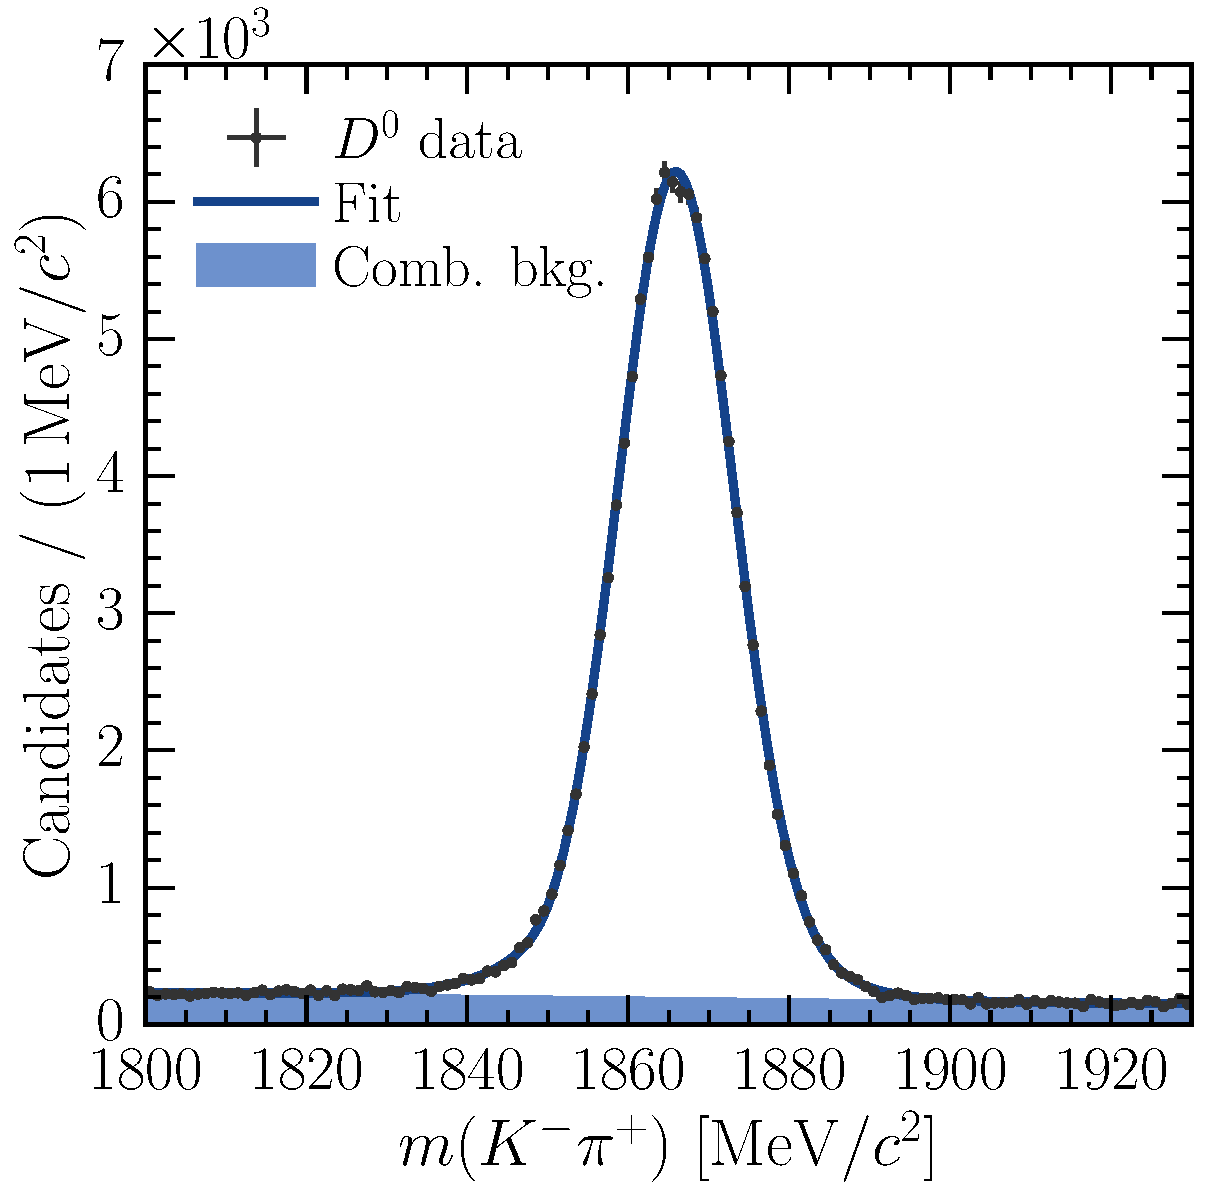
\includegraphics[width=\textwidth]{production/fitting/D0ToKpi_mass_fit_pT_3_y_2}
    \caption{Mass}
    \label{fig:prod:fitting:D0ToKpi:mass_high_sig}
  \end{subfigure}
  \begin{subfigure}[b]{0.5\textwidth}
    \centering
    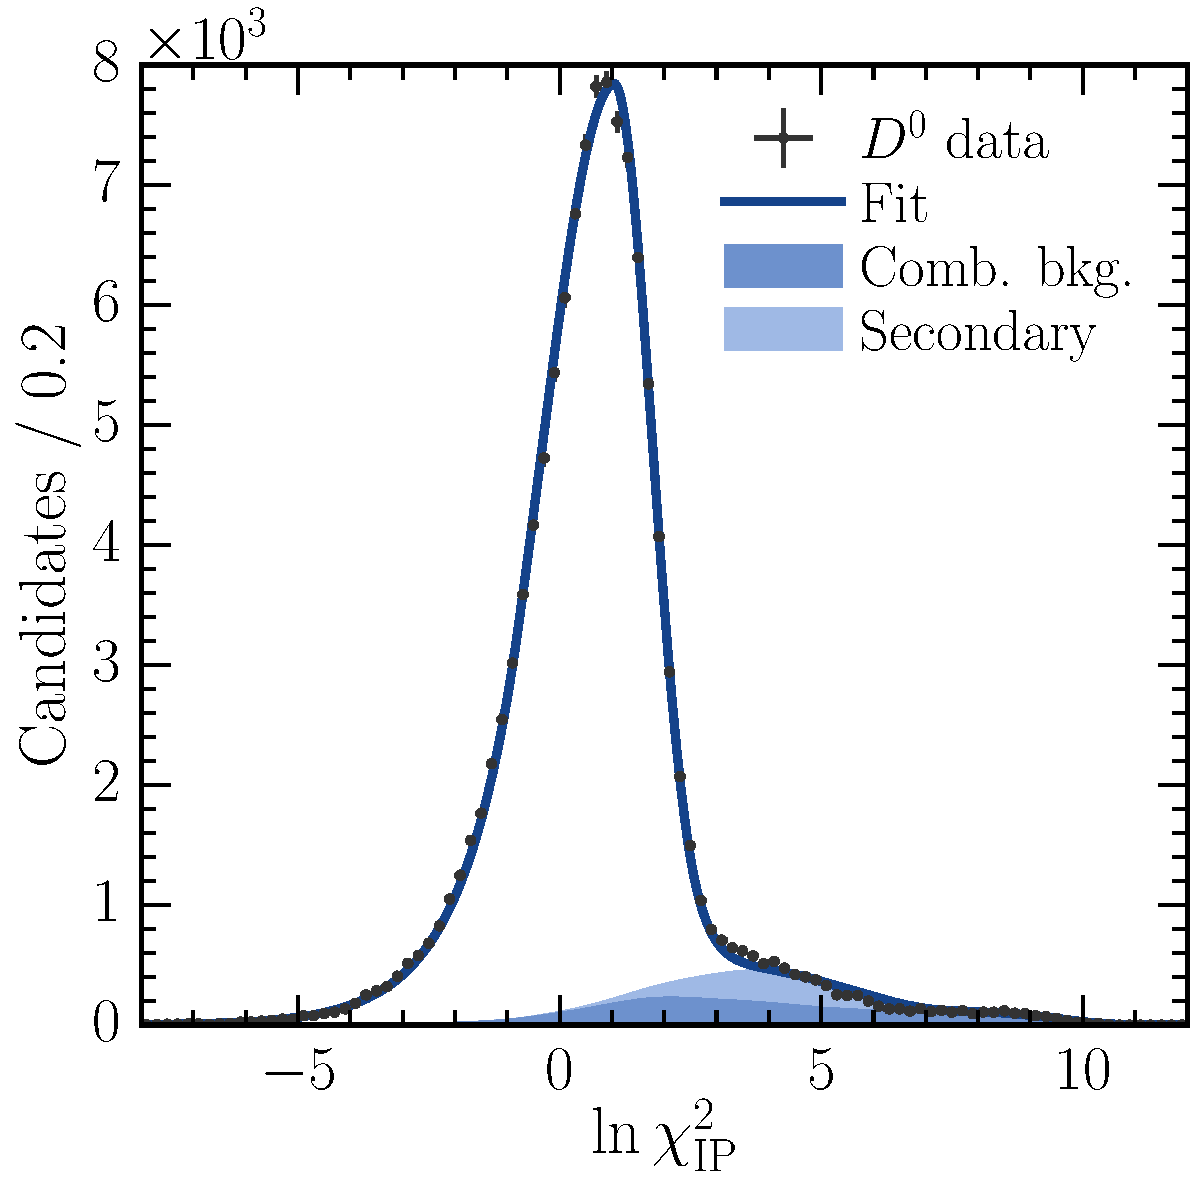
\includegraphics[width=\textwidth]{production/fitting/D0ToKpi_ipchisq_fit_pT_3_y_2}
    \caption{\lnipchisq}
    \label{fig:prod:fitting:D0ToKpi:ipchisq_high_sig}
  \end{subfigure}
  \begin{subfigure}[b]{0.5\textwidth}
    \centering
    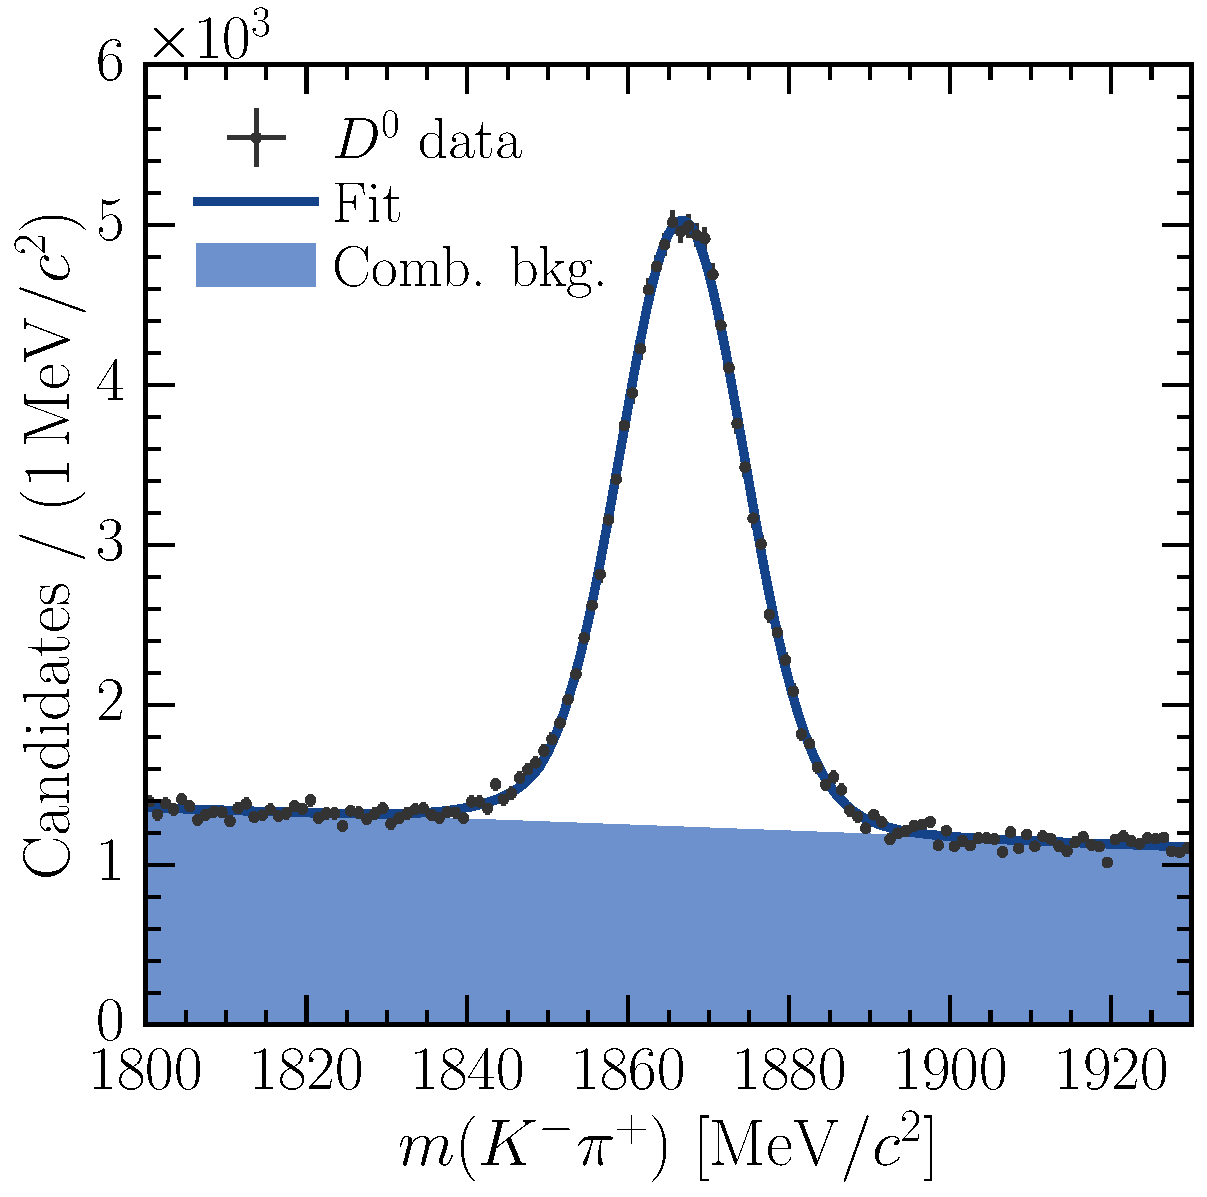
\includegraphics[width=\textwidth]{production/fitting/D0ToKpi_mass_fit_pT_0_y_3}
    \caption{Mass}
    \label{fig:prod:fitting:D0ToKpi:mass_high_bkg}
  \end{subfigure}
  \begin{subfigure}[b]{0.5\textwidth}
    \centering
    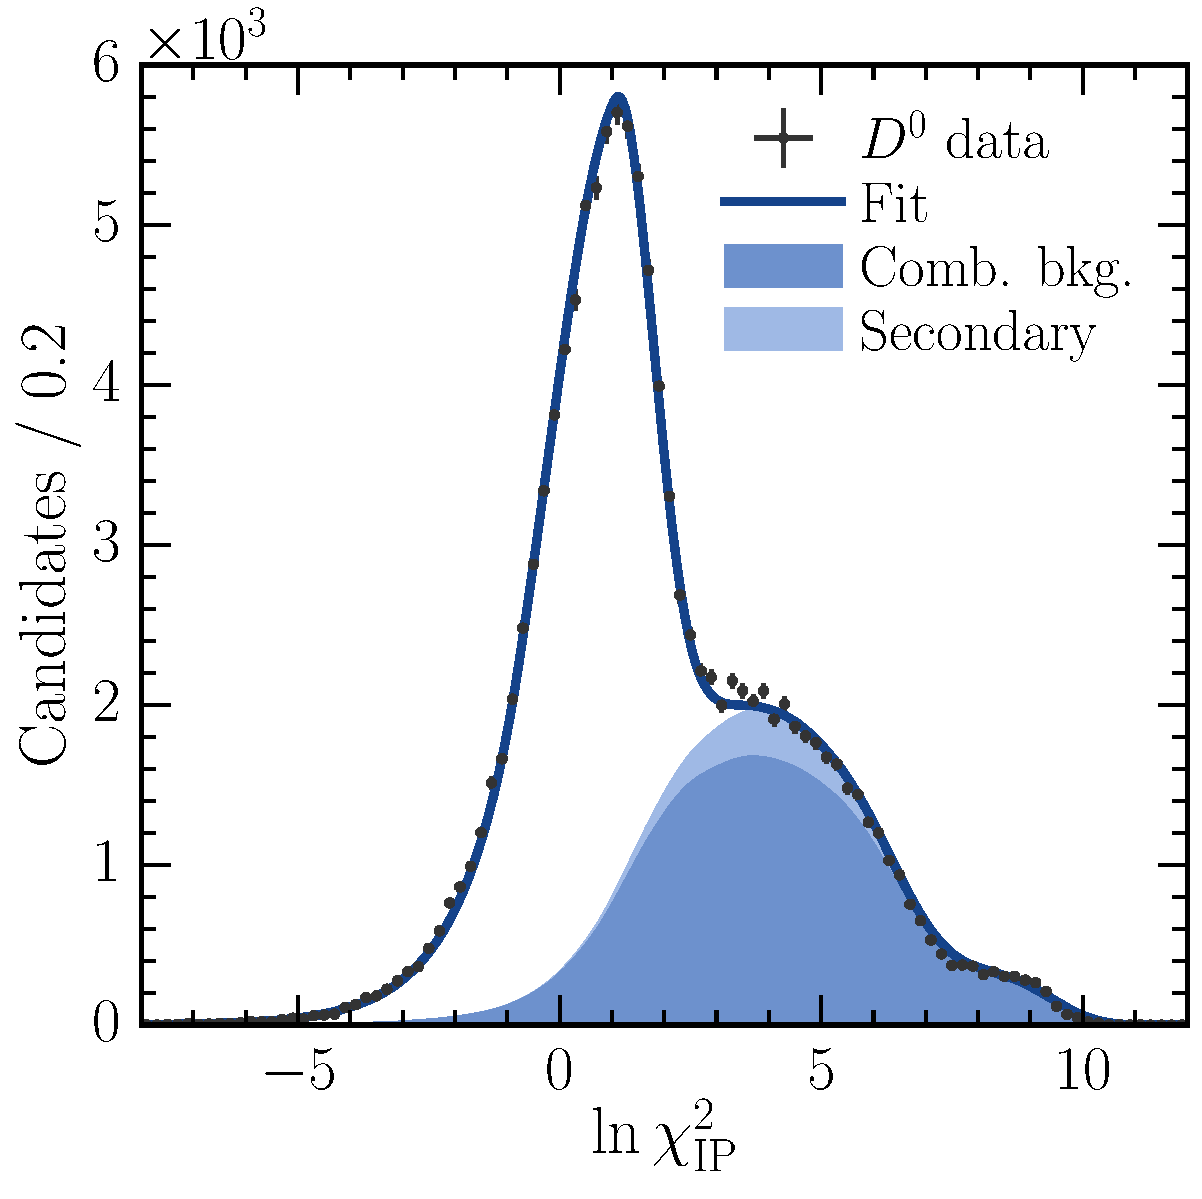
\includegraphics[width=\textwidth]{production/fitting/D0ToKpi_ipchisq_fit_pT_0_y_3}
    \caption{\lnipchisq}
    \label{fig:prod:fitting:D0ToKpi:ipchisq_high_bkg}
  \end{subfigure}
  \caption{%
    Distributions for fully selected \DzToKpi\ candidates: \PDzero\ invariant 
    mass (\subref*{fig:prod:fitting:D0ToKpi:mass_high_sig} and 
    \subref*{fig:prod:fitting:D0ToKpi:mass_high_bkg}); and \PDzero\ \lnipchisq\ 
    (\subref*{fig:prod:fitting:D0ToKpi:ipchisq_high_sig} and 
    \subref*{fig:prod:fitting:D0ToKpi:ipchisq_high_bkg}) for a mass window of 
    $\pm\SI{20}{\MeVcc}$ around the nominal \PDzero mass.
    The top Figures (\subref*{fig:prod:fitting:D0ToKpi:mass_high_sig} and 
    \subref*{fig:prod:fitting:D0ToKpi:ipchisq_high_sig}) show the data and fits 
    in the region \pTyrange{2}{2.5}{3}{3.5}, whilst the bottom Figures 
    (\subref*{fig:prod:fitting:D0ToKpi:mass_high_bkg} and 
    \subref*{fig:prod:fitting:D0ToKpi:ipchisq_high_bkg}) show the data and fits 
    in the \pTyrange{0}{1}{3.5}{4} region.
  }
  \label{fig:prod:fitting:D0ToKpi:sig_bkg}
\end{figure}

\begin{figure}
  \begin{subfigure}[b]{0.5\textwidth}
    \centering
    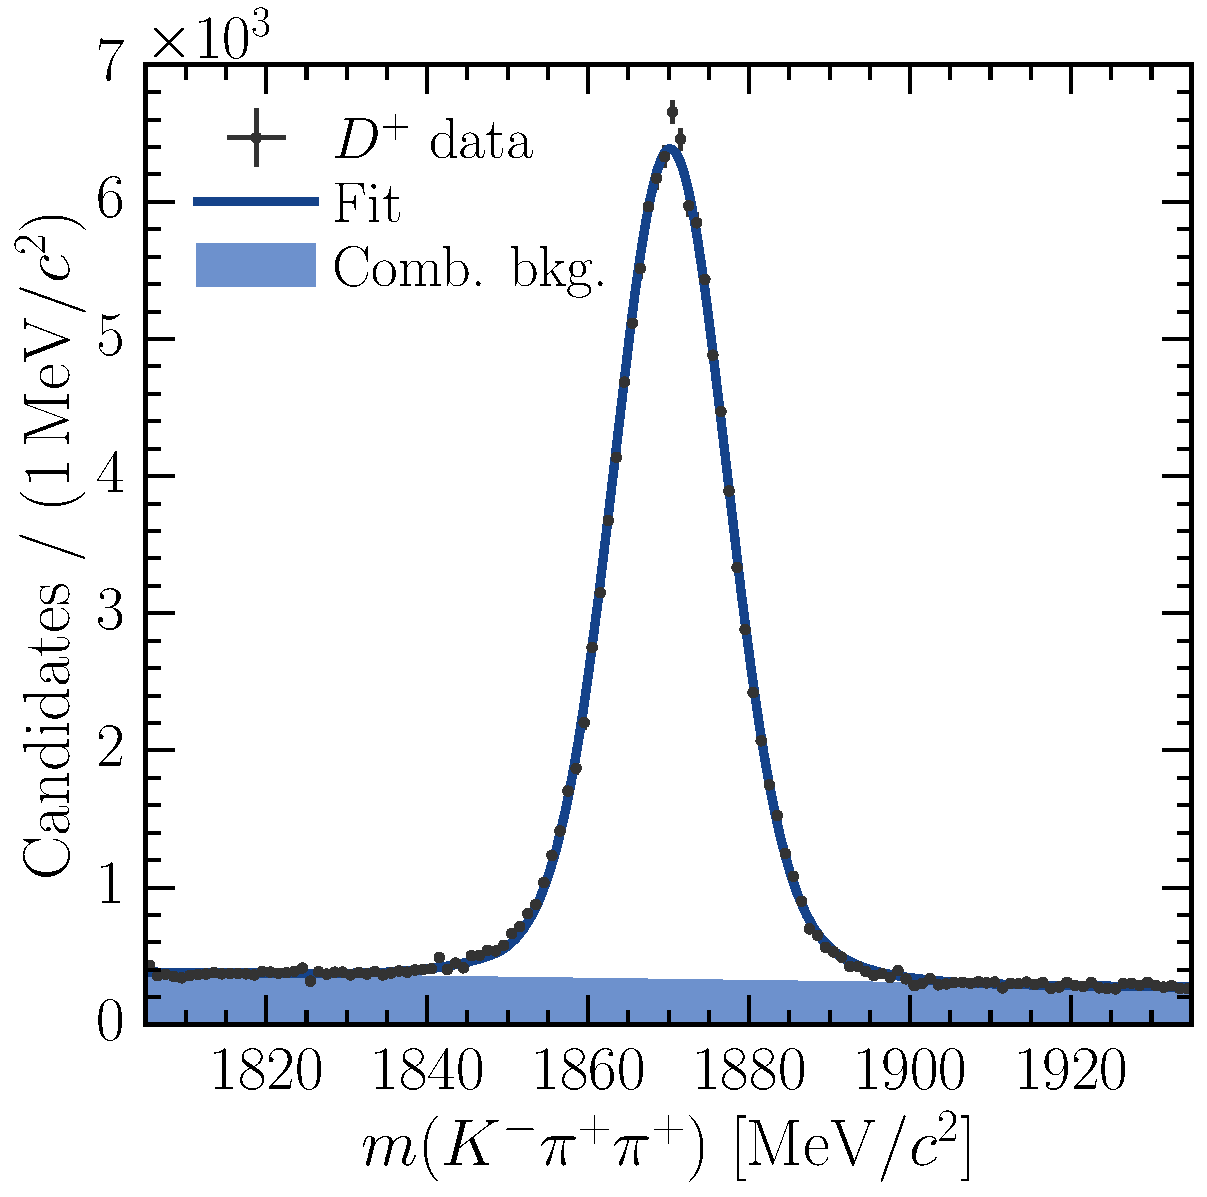
\includegraphics[width=\textwidth]{production/fitting/DpToKpipi_mass_fit_pT_4_y_2}
    \caption{Mass}
    \label{fig:prod:fitting:DpToKpipi:mass_high_sig}
  \end{subfigure}
  \begin{subfigure}[b]{0.5\textwidth}
    \centering
    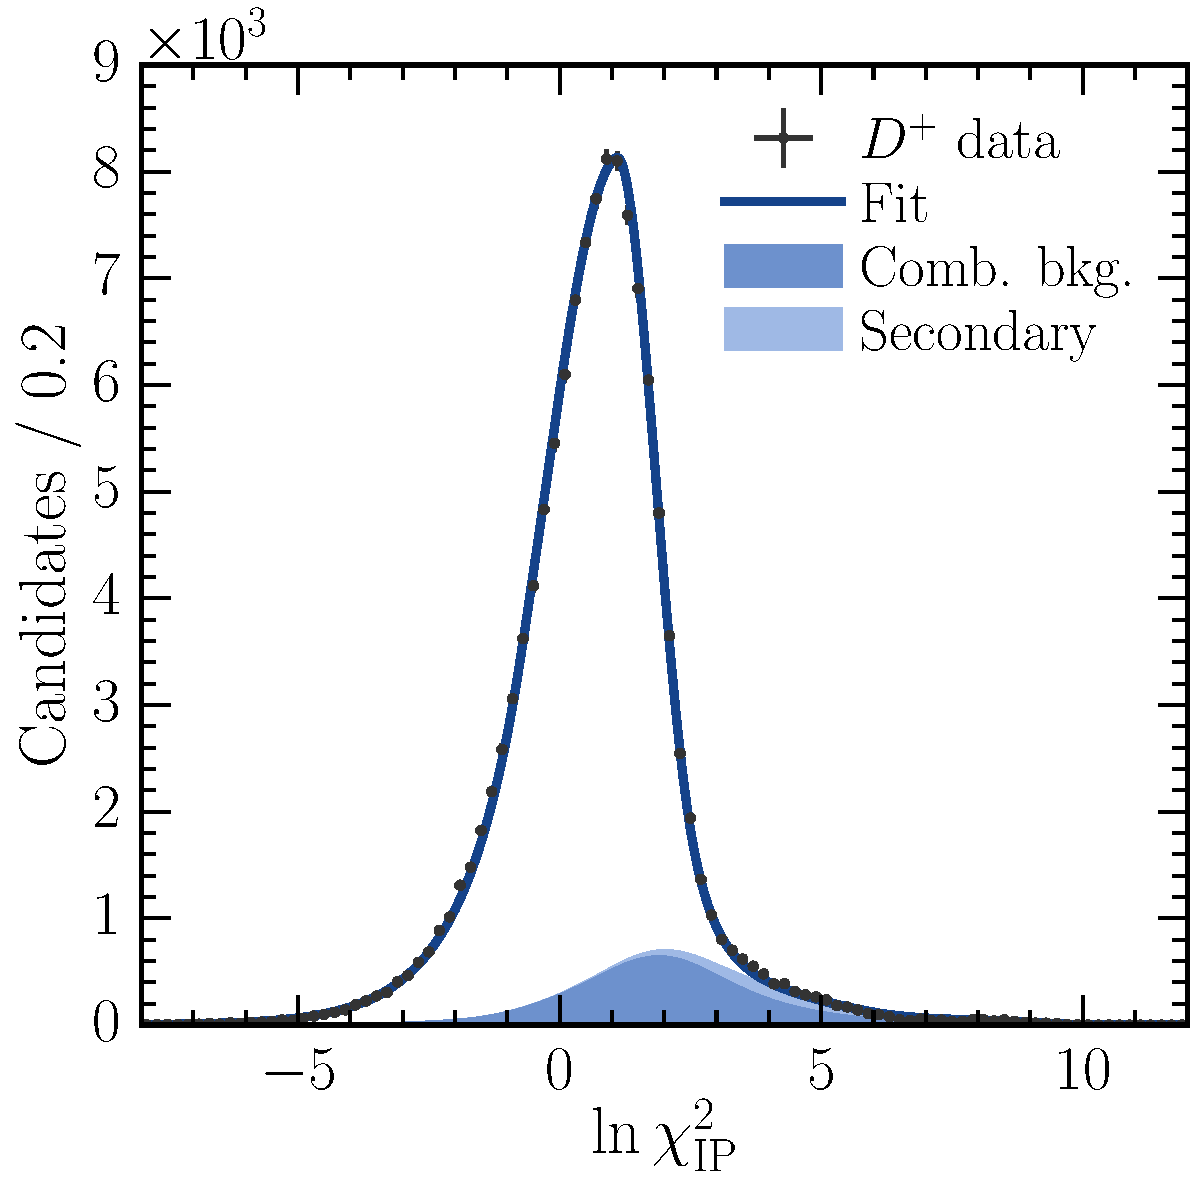
\includegraphics[width=\textwidth]{production/fitting/DpToKpipi_ipchisq_fit_pT_4_y_2}
    \caption{\lnipchisq}
    \label{fig:prod:fitting:DpToKpipi:ipchisq_high_sig}
  \end{subfigure}
  \begin{subfigure}[b]{0.5\textwidth}
    \centering
    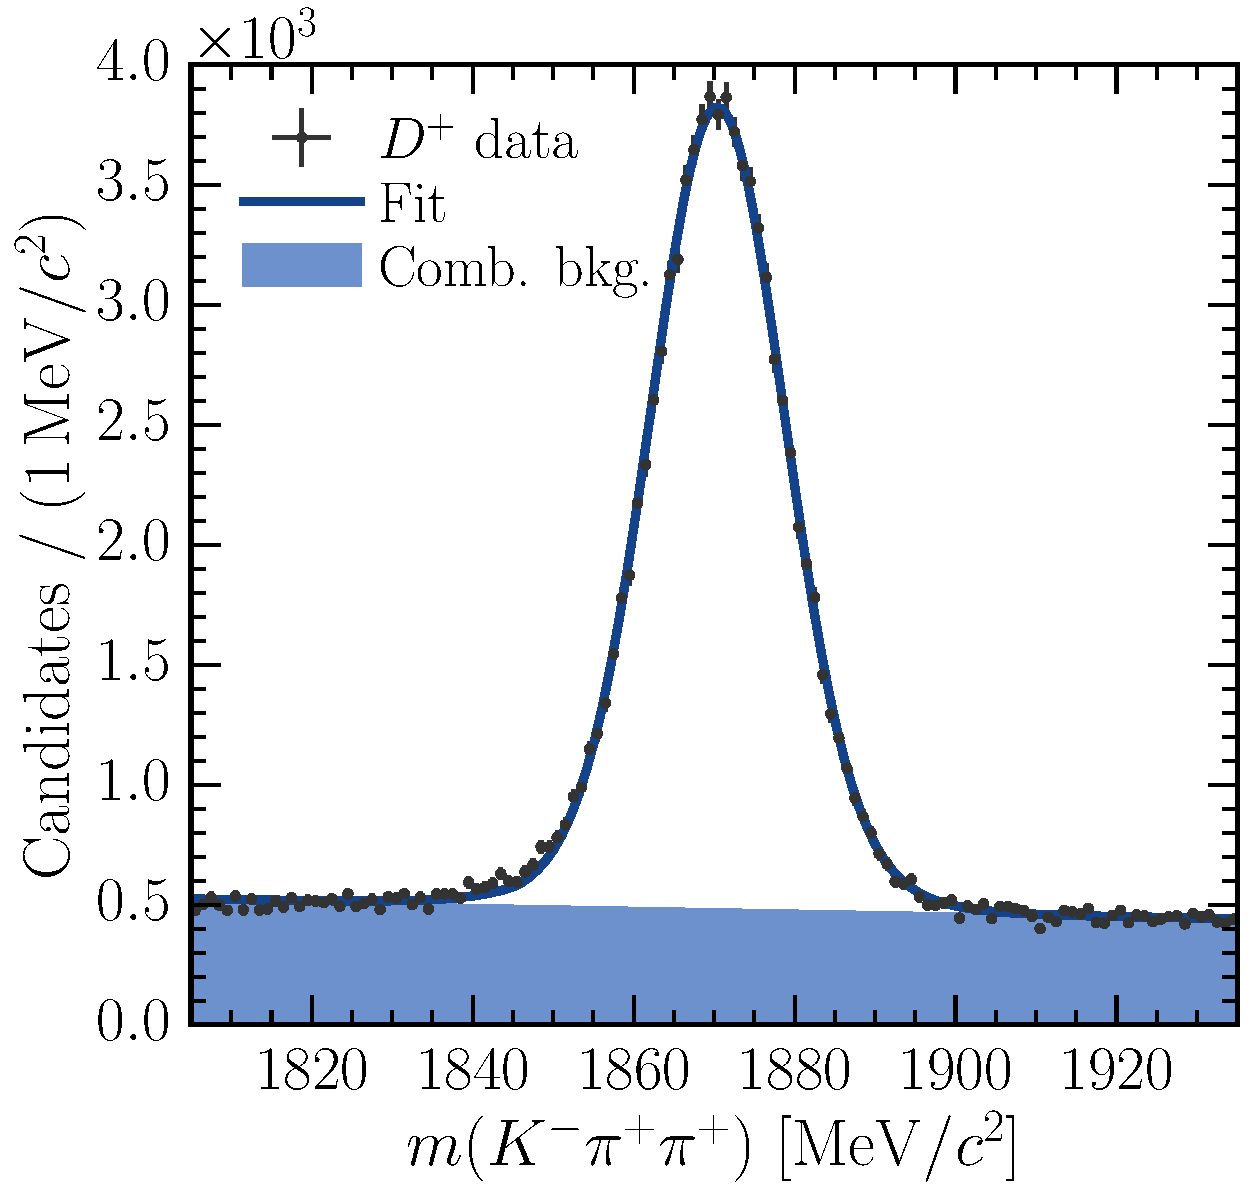
\includegraphics[width=\textwidth]{production/fitting/DpToKpipi_mass_fit_pT_3_y_3}
    \caption{Mass}
    \label{fig:prod:fitting:DpToKpipi:mass_high_bkg}
  \end{subfigure}
  \begin{subfigure}[b]{0.5\textwidth}
    \centering
    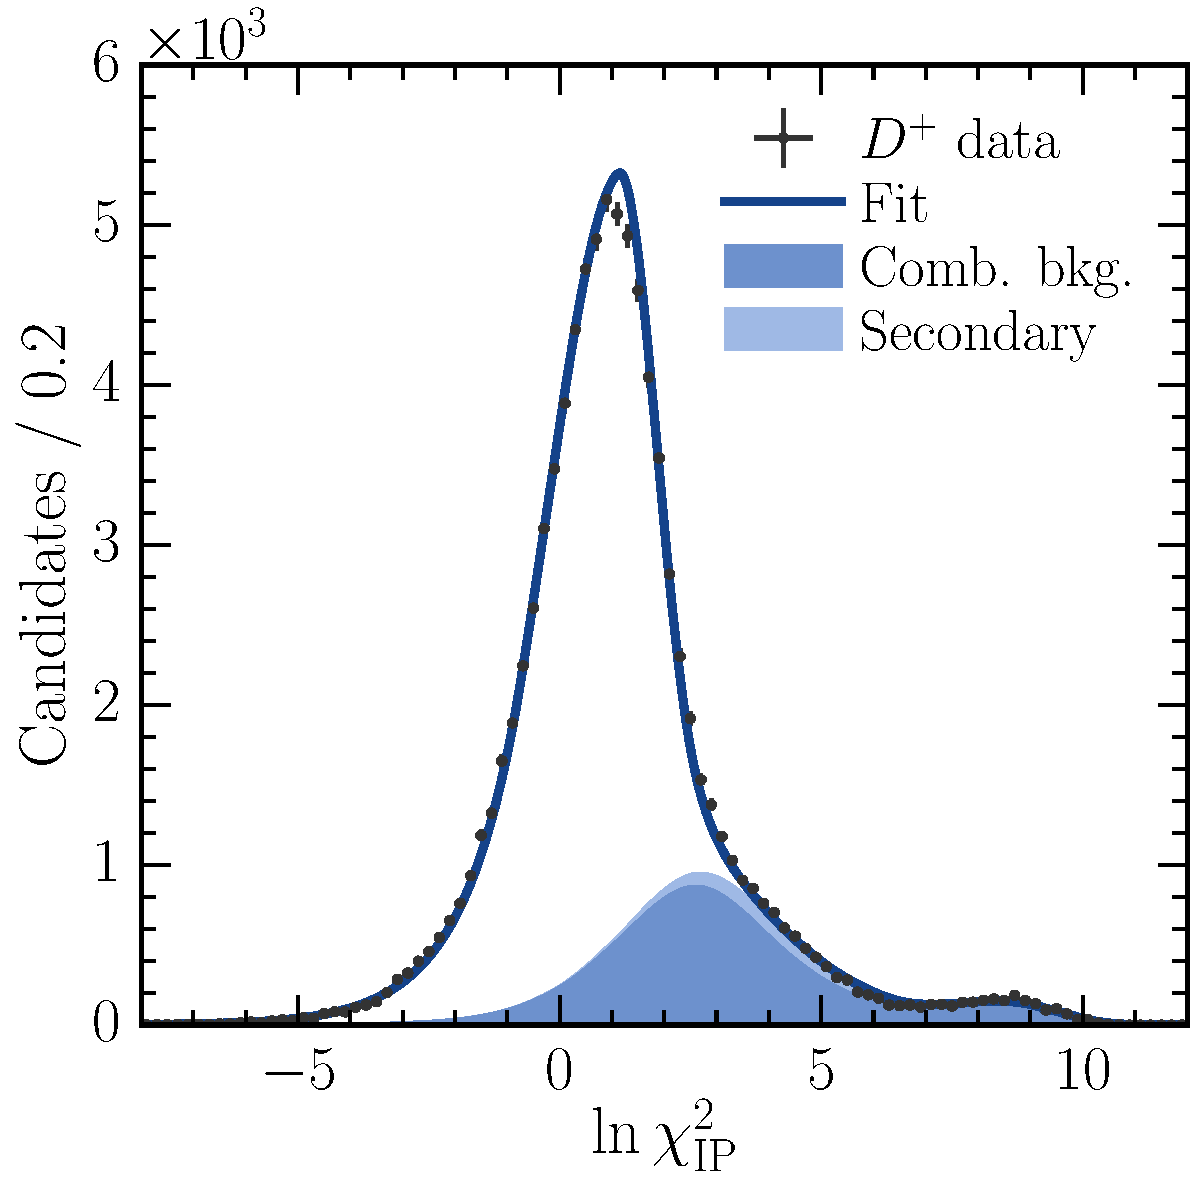
\includegraphics[width=\textwidth]{production/fitting/DpToKpipi_ipchisq_fit_pT_3_y_3}
    \caption{\lnipchisq}
    \label{fig:prod:fitting:DpToKpipi:ipchisq_high_bkg}
  \end{subfigure}
  \caption{%
    Distributions for fully selected \DpToKpipi\ candidates: \PDplus\ invariant 
    mass (\subref*{fig:prod:fitting:DpToKpipi:mass_high_sig} and 
    \subref*{fig:prod:fitting:DpToKpipi:mass_high_bkg}); and \PDplus\ 
    \lnipchisq\ (\subref*{fig:prod:fitting:DpToKpipi:ipchisq_high_sig} and 
    \subref*{fig:prod:fitting:DpToKpipi:ipchisq_high_bkg}) for a mass window of 
    $\pm\SI{20}{\MeVcc}$ around the nominal \PDplus mass.
    The top Figures (\subref*{fig:prod:fitting:DpToKpipi:mass_high_sig} and 
    \subref*{fig:prod:fitting:DpToKpipi:ipchisq_high_sig}) show the data and 
    fits in the region \pTyrange{2.5}{3}{3}{3.5}, whilst the bottom Figures 
    (\subref*{fig:prod:fitting:DpToKpipi:mass_high_bkg} and 
    \subref*{fig:prod:fitting:DpToKpipi:ipchisq_high_bkg}) show the data and 
    fits in the \pTyrange{2}{2.5}{3.5}{4} region.
  }
  \label{fig:prod:fitting:DpToKpipi:sig_bkg}
\end{figure}

\begin{figure}
  \begin{subfigure}[b]{0.5\textwidth}
    \centering
    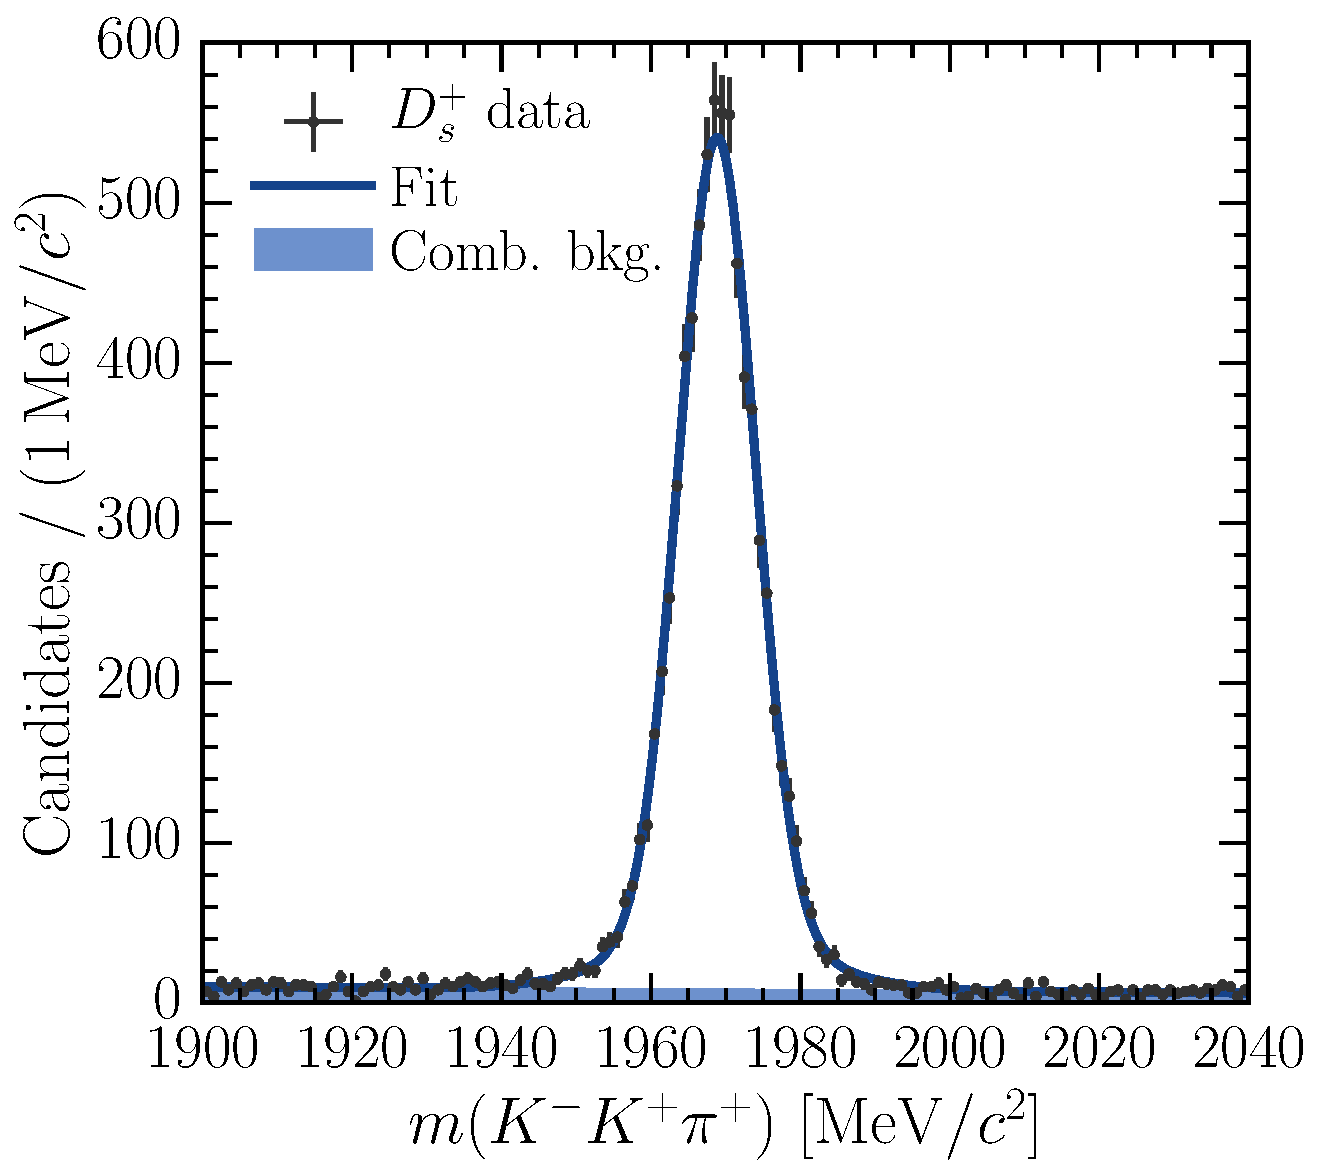
\includegraphics[width=\textwidth]{production/fitting/DsToKKpi_mass_fit_pT_6_y_1}
    \caption{Mass}
    \label{fig:prod:fitting:DsToKKpi:mass_high_sig}
  \end{subfigure}
  \begin{subfigure}[b]{0.5\textwidth}
    \centering
    \includegraphics[width=\textwidth]{production/fitting/DsToKKpi_ipchisq_fit_pT_6_y_1}
    \caption{\lnipchisq}
    \label{fig:prod:fitting:DsToKKpi:ipchisq_high_sig}
  \end{subfigure}
  \begin{subfigure}[b]{0.5\textwidth}
    \centering
    \includegraphics[width=\textwidth]{production/fitting/DsToKKpi_mass_fit_pT_2_y_3}
    \caption{Mass}
    \label{fig:prod:fitting:DsToKKpi:mass_high_bkg}
  \end{subfigure}
  \begin{subfigure}[b]{0.5\textwidth}
    \centering
    \includegraphics[width=\textwidth]{production/fitting/DsToKKpi_ipchisq_fit_pT_2_y_3}
    \caption{\lnipchisq}
    \label{fig:prod:fitting:DsToKKpi:ipchisq_high_bkg}
  \end{subfigure}
  \caption{%
    Distributions for fully selected \DspTophipi\ candidates: \PDsplus\ 
    invariant mass (\subref*{fig:prod:fitting:DsToKKpi:mass_high_sig} and 
    \subref*{fig:prod:fitting:DsToKKpi:mass_high_bkg}); and \PDsplus\ 
    \lnipchisq\ (\subref*{fig:prod:fitting:DsToKKpi:ipchisq_high_sig} and 
    \subref*{fig:prod:fitting:DsToKKpi:ipchisq_high_bkg}) for a mass window of 
    $\pm\SI{20}{\MeVcc}$ around the nominal \PDsplus mass.
    The top Figures (\subref*{fig:prod:fitting:DsToKKpi:mass_high_sig} and 
    \subref*{fig:prod:fitting:DsToKKpi:ipchisq_high_sig}) show the data and 
    fits in the region \pTyrange{4}{5}{2.5}{3}, whilst the bottom Figures 
    (\subref*{fig:prod:fitting:DsToKKpi:mass_high_bkg} and 
    \subref*{fig:prod:fitting:DsToKKpi:ipchisq_high_bkg}) show the data and 
    fits in the \pTyrange{2}{2.5}{3.5}{4} region.
  }
  \label{fig:prod:fitting:DsToKKpi:sig_bkg}
\end{figure}

\begin{figure}
  \begin{subfigure}[b]{0.5\textwidth}
    \centering
    \includegraphics[width=\textwidth]{production/fitting/DstToD0pi_D0ToKpi_delta_mass_fit_pT_7_y_2}
    \caption{Delta mass}
    \label{fig:prod:fitting:DstToD0pi_D0ToKpi:delta_mass_high_sig}
  \end{subfigure}
  \begin{subfigure}[b]{0.5\textwidth}
    \centering
    \includegraphics[width=\textwidth]{production/fitting/DstToD0pi_D0ToKpi_ipchisq_fit_pT_7_y_2}
    \caption{\lnipchisq}
    \label{fig:prod:fitting:DstToD0pi_D0ToKpi:ipchisq_high_sig}
  \end{subfigure}
  \begin{subfigure}[b]{0.5\textwidth}
    \centering
    \includegraphics[width=\textwidth]{production/fitting/DstToD0pi_D0ToKpi_delta_mass_fit_pT_2_y_3}
    \caption{Delta mass}
    \label{fig:prod:fitting:DstToD0pi_D0ToKpi:delta_mass_high_bkg}
  \end{subfigure}
  \begin{subfigure}[b]{0.5\textwidth}
    \centering
    \includegraphics[width=\textwidth]{production/fitting/DstToD0pi_D0ToKpi_ipchisq_fit_pT_2_y_3}
    \caption{\lnipchisq}
    \label{fig:prod:fitting:DstToD0pi_D0ToKpi:ipchisq_high_bkg}
  \end{subfigure}
  \caption{%
    Distributions for fully selected \DstToDzpi, with \DzToKpi, candidates: 
    $\deltam = m(\PDstarp) - m(\PDzero)$ 
    (\subref*{fig:prod:fitting:DstToD0pi_D0ToKpi:delta_mass_high_sig} and 
    \subref*{fig:prod:fitting:DstToD0pi_D0ToKpi:delta_mass_high_bkg}) for a 
    mass window of $\pm\SI{20}{\MeVcc}$ around the nominal \PDzero mass; and 
    \PDzero\ \lnipchisq\ 
    (\subref*{fig:prod:fitting:DstToD0pi_D0ToKpi:ipchisq_high_sig} and 
    \subref*{fig:prod:fitting:DstToD0pi_D0ToKpi:ipchisq_high_bkg}) with an 
    additional mass window of $\pm\SI{3}{\MeVcc}$ around the nominal 
    \PDstarp-\PDzero\ mass difference.
    The top Figures 
    (\subref*{fig:prod:fitting:DstToD0pi_D0ToKpi:delta_mass_high_sig} and 
    \subref*{fig:prod:fitting:DstToD0pi_D0ToKpi:ipchisq_high_sig}) show the 
    data and fits in the region \pTyrange{4}{5}{3}{3.5}, whilst the bottom 
    Figures (\subref*{fig:prod:fitting:DstToD0pi_D0ToKpi:delta_mass_high_bkg} 
    and \subref*{fig:prod:fitting:DstToD0pi_D0ToKpi:ipchisq_high_bkg}) show the 
    data and fits in the \pTyrange{1.5}{2}{3.5}{4} region.
  }
  \label{fig:prod:fitting:DstToD0pi_D0ToKpi:sig_bkg}
\end{figure}


\chapter{Efficiency evaluation}
\label{chap:prod:effs}

The efficiency chain defines the fraction of prompt charm mesons that survive 
the full reconstruction and selection procedure.
The chain is defined in steps grouped by physical requirements and those 
imposed by software, with each step being relative to the previous one.
This starts with the efficiency of a signal charm hadron to decay within the 
\lhcb\ acceptance having been produced in a \pp\ collision, \effacc.
The efficiency of such a decay to be fully reconstructed is the reconstruction 
efficiency is \effreco, and then the efficiency of the reconstructed decay to 
be triggered through \lzero, \hltone, and \hlttwo\ is the trigger efficiency 
\efftrig.
There is also the efficiency of triggered candidates to pass through the 
offline selection \effoffline, and finally there is the signal window 
efficiency \effsigwin\ due to the requirement imposed before the \lnipchisq\ 
fit.
The total efficiency, \eff, is the product of these, and is what enters in 
\cref{eqn:prod:introduction:differential_cross_section}.

Two methods are used for efficiency estimation: using the \acf{MC} data, where 
true information is available before and after all steps; and methods of 
calibration, where proxy data selected without the use of particular 
information can be used to assess the effects of using that information in the 
analysis data.
Efficiency evaluation with \ac{MC} can be simple, but differences between the 
data and the \ac{MC} must be accounted for, which may not be obvious.
Calibration techniques use real data, and so can be more robust than \ac{MC}, 
but obtaining clean calibration samples can be challenging.

In \lhcb, it is known that the \ac{PID} selection efficiencies are not 
well-modelled in the \ac{MC} due to an under-estimation of the detector 
occupancies.
The same is true, albeit to a lesser extent, for the reconstruction 
efficiencies.
Kinematic variables, such as charm hadron and final state momenta, are 
comparatively well-modelled.
This motivates a two-step procedure for evaluating the \emph{selection} 
efficiency, whereby the \ac{PID} efficiency is computed using calibration 
techniques, described in \cref{chap:prod:effs:pid}, and the efficiency of the remaining 
requirements is made using \ac{MC}, detailed in \cref{chap:prod:effs:sel}.
The reconstruction efficiency will be computed using \ac{MC}, but corrected 
with a factor obtained from calibration samples, described in \cref{chap:prod:effs:acc}.
The extent to which these techniques do not accurately model the efficiencies 
will be discussed in the context of systematic uncertainties in 
\cref{chap:prod:syst:mc}.

The matching of true \ac{MC} particles to reconstructed objects, the process of 
truth-matching as described in \cref{chap:prod:data:mc}, is not \SI{100}{\%} 
efficient, and so a correction factor \efftruth\ is be computed to account for 
the deficit.

To summarise: the total efficiency $\eff_{i}(\decay{\PHc}{f})$, for charm 
candidates in the $i$th \pTy\ bin, is the product of the individual 
efficiencies and correction factors
\begin{align}
  \eff_{i}(\decay{\PHc}{f}) = \effacc &\times \effreco \times \efftruth \times \efftracking \nonumber\\
                                      &\times \efftrig \times \effoffline \times \effpid \times \effsigwin.
  \label{eqn:prod:effs:total_eff}
\end{align}
where each efficiency \eff\ is dependent on the charm hadron \PHc\ and the 
final state $f$, and is conditional on the previous step.

In this \namecref{chap:prod:effs} the details of the efficiency computation for 
each step are given, along with example efficiency tables in \pTy\ for the 
two-body \DzToKpi\ and three-body \DpToKpipi\ decays.
The notation for conditional yields will be used throughout, where $N_{B|A}$ 
denotes the prompt signal yield after process $B$ given that process $A$ 
preceded $B$.

\section{Detector acceptance}
\label{chap:prod:effs:acc}

The acceptance efficiency is due to the finite spatial acceptance of the \lhcb\ 
detector.
There is no way to access these particles in data, and so simulated data is 
used.
The acceptance is modelled by a set of cuts requiring that all stable charged 
particles in the final state have a momentum direction satisfying $10 < \theta 
< \SI{400}{\milli\radian}$, and that all the particles in the final state point 
in the positive $z$ direction.
These requirements are applied at the generator level, before the detector 
simulation, on the true kinematics of the particles.

By counting the number of prompt charm hadrons passing and failing the cut, the 
acceptance efficiency is defined as
\begin{equation}
  \effacc = \frac{%
    N_{\text{Accepted}|\text{Generated}}
  }
  {%
    N_{\text{\text{Generated}}}
  }.
  \label{eqn:prod:effs:acc}
\end{equation}
The input dataset to this computation is the generator-level set described in 
\cref{chap:prod:data:mc}.
The acceptance efficiencies for \DzToKpi\ and \DpToKpipi, in \pTy\ bins, are 
given in \cref{tab:prod:effs:acc:dztokpi,tab:prod:effs:acc:dptokpipi}.

\section{Reconstruction}
\label{chap:prod:effs:reco}

The reconstruction efficiency \effreco\ parameterises the fraction of charm 
meson decays passing the acceptance requirements that are also fully 
reconstructed as tracks, for the final state particles, and vertices, for the 
charm mesons.
This folds in several effects: whether the final state particles have a large 
enough momentum not to be bent out of the detector acceptance by the magnetic 
field; whether the final state particles leave enough hits in the tracking 
system to be reconstructible (that is, above the minimum threshold at which the 
tracking system \emph{could} reconstruct a track); whether, given that enough 
hits were deposited by a final state particle, a track was actually 
reconstructed; and whether a vertex can be formed, given that all final state 
particles have associated tracks.

The reconstruction efficiency is defined as the ratio of fully reconstructed 
decays to those passing the acceptance requirements
\begin{equation}
  \effreco = \frac{%
    N_{\text{Reconstructed}|\text{Accepted}}
  }
  {%
    N_{\text{\text{Accepted}}}
  }.
  \label{eqn:prod:effs:reco}
\end{equation}
The reconstruction efficiencies for \DzToKpi\ and \DpToKpipi, in \pTy\ bins, are 
given in \cref{tab:prod:effs:reco:dztokpi,tab:prod:effs:reco:dptokpipi}.

\subsection{Truth matching inefficiency}
\label{chap:prod:effs:truth}

The evaluation of \cref{eqn:prod:effs:reco} requires that the reconstructed 
objects, tracks and vertices, be correctly associated back to the `truth-level' 
information, that is the \ac{MC} objects which were generated and then 
propagated through the detector simulation.
The truth-matching procedure is described in \cref{chap:prod:data:mc}.
The background category information is used to filter the \ac{MC} such that the 
number of remaining candidates are counted to obtain the input to some 
efficiency computation, such as \cref{eqn:prod:effs:reco}.
However, the requirement that a track is matched to \SI{70}{\percent} of the 
hits created by an \ac{MC} particle is not \SI{100}{\percent} efficient at 
accepting signal.
The magnitude of the size of the inefficiency can be determined by counting the 
number of signal decays that fail the truth matching requirement.
\cref{fig:prod:effs:truth:categories} shows the \PDzero and \PDplus mass 
distributions for the various background categories.
The `ghost' category exhibits a peak identical in nature to that seen in the 
`signal' category.
As not all signal decays that are truly reconstructed will be counted as such 
when only the `signal' category is considered, associated efficiencies are 
underestimated, leading to an overestimation of the cross-section.

Given that the number of correctly matched signal decays is $N$, and the number 
of incorrectly labelled signal decays is $U$, the selection efficiency defined 
in \cref{eqn:prod:effs:reco} is incorrect by a factor
\begin{equation}
  \efftruth = \frac{U+N}{N}.
  \label{eqn:prod:effs:truth}
\end{equation}
The number of decays passing the signal requirement is used for $N$, and $U$ is 
measured with a maximum likelihood fit to the mass or \deltam\ distribution of 
the decays not passing the requirement.
As shown in \cref{fig:prod:effs:truth:categories}, the fraction of incorrectly 
identified signal decays is small, and so a single fit is performed with the 
data integrated across all \pTy\ bins, and a single correction factor is 
measured.
The details of the fit are identical to those for the mass fits used in the 
prompt charm yield extraction with real data, described in 
\cref{chap:prod:fitting:mass}.
The result of the fits to the \DzToKpi\ and the \DpToKpipi\ simulated datasets 
are shown in \cref{fig:prod:effs:truth:fit}.
Table~\ref{tab:prod:effs:truth_matching} lists the obtained correction factors.

\begin{figure}
  \begin{subfigure}[b]{0.5\textwidth}
    \centering
    \includegraphics[width=\textwidth]{production/efficiencies/D0ToKpi_BKGCAT}
    \caption{\PDzero}
    \label{fig:prod:effs:truth:categories:D0ToKpi}
  \end{subfigure}
  \begin{subfigure}[b]{0.5\textwidth}
    \centering
    \includegraphics[width=\textwidth]{production/efficiencies/DpToKpipi_BKGCAT}
    \caption{\PDplus}
    \label{fig:prod:effs:truth:categories:DpToKpipi}
  \end{subfigure}
  \caption{%
    Mass distributions of \ac{MC} 
    \PDzero~(\subref*{fig:prod:effs:truth:categories:D0ToKpi}) and 
    \PDplus~(\subref*{fig:prod:effs:truth:categories:DpToKpipi}) candidates for 
    various background categories, as indicated in the legends.
    The most prominent features are the signal-like peak in the `ghost' 
    distribution, indicative of a truth-matching inefficiency, and the long 
    tail extending below the mass peak in the `other' distribution, which 
    mostly consists of partially reconstructed physics backgrounds such as 
    \decay{\PDzero}{\PKminus\Ppiplus\Ppizero} and 
    \decay{\PDplus}{\PKminus\Ppiplus\Ppiplus\Ppizero}.
  }
  \label{fig:prod:effs:truth:categories}
\end{figure}

\begin{figure}
  \begin{subfigure}[b]{0.5\textwidth}
    \centering
    \includegraphics[width=\textwidth]{production/efficiencies/D0ToKpi_BKGCAT_fit}
    \caption{\DzToKpi}
    \label{fig:prod:effs:truth:fit:D0ToKpi}
  \end{subfigure}
  \begin{subfigure}[b]{0.5\textwidth}
    \centering
    \includegraphics[width=\textwidth]{production/efficiencies/DpToKpipi_BKGCAT_fit}
    \caption{\DpToKpipi}
    \label{fig:prod:effs:truth:fit:DpToKpipi}
  \end{subfigure}
  \caption{%
    Mass distributions of \ac{MC} 
    \PDzero~(\subref*{fig:prod:effs:truth:fit:D0ToKpi}) and 
    \PDplus~(\subref*{fig:prod:effs:truth:fit:DpToKpipi}) candidates not 
    passing the `signal' truth-matching requirement, that is the sum of the 
    ``Ghost'' and ``Other'' categories shown in 
    \cref{fig:prod:effs:truth:categories}.
    Overlaid on each distribution is the result of a maximum likelihood fit, 
    with the total model shown as a blue curve, and the background model as a 
    red dotted line.
  }
  \label{fig:prod:effs:truth:fit}
\end{figure}

\subsection{Tracking efficiency correction}
\label{chap:prod:effs:tracking}

The track reconstruction efficiency, or tracking efficiency, measures the 
efficiency for a charged particle to be reconstructed as a track, and is part 
of the definition of the reconstruction efficiency in 
\cref{eqn:prod:effs:reco}.
The \ac{MC} may not accurately model the tracking efficiency, and so a 
data-driven technique is used to compute correction factors based on the 
observed differences between the data and the \ac{MC}.

Only long tracks are used in this analysis, which requires that the particles 
create hits in the \velo\ and in the T stations.
Hits in the \ttracker\ are not required to form long tracks, although matching 
hits are added to tracks to improve their momentum resolution.
To measure the efficiency of long track creation, \JpsiTomumu\ decays are 
reconstructed using a `tag-and-probe' technique, where one particle is fully 
reconstructed as a long track, as usual, and the other track is created using 
track segments made only using information from the muon stations.
The momentum of the latter track, the `probe', can be inferred by treating the 
magnetic field as an optical system that imparts a momentum `kick' in the $x$ 
direction.
By assuming the muon track segment was made by a particle originating from the 
\ac{PV}, the probe segment can be extrapolated back from the muon stations to 
the $yz$ plane where the kick is modelled, and then the difference in slopes 
between the \ac{PV}-plane line and the probe track gives the probe momentum.
The invariant mass of the dimuon system can then be computed, the distribution 
for many tag-and-probe candidates can be used to distinguish between 
backgrounds and true \PJpsi decays.
The mass resolution of \JpsiTomumu\ decays reconstructed using long+muon tracks 
is about \SI{200}{\MeVcc}, to be compared with a resolution of about 
\SI{16}{\MeVcc} using long+long tracks.
To improve the mass resolution, the muon tracks are combined with hits in the 
\ttracker, improving the resolution to around 
\SI{57}{\MeVcc}~\cite{Aaij:2014pwa,DeCian:2013zua}.

The tracking efficiency is evaluated as the ratio of \PJpsi mesons 
reconstructed using the long+muon+\ttracker\ method, with those that can 
\emph{also} be reconstructed using the long+long method
\begin{equation}
  \eff_{\text{Tracking}} = 
  \frac{%
    N_{\text{long+long}|\text{long+muon+TT}}
  }{%
    N_{\text{long+muon+TT}}
  }.
  \label{eqn:prod:effs:tracking_eff}
\end{equation}
A long track in an event is considered as `matched' to the probe track if there 
is a \SI{70}{\percent} overlap of their hits in the muon stations.
The tag-and-probe method is performed using real data and \ac{MC}, and a ratio 
is formed
\begin{equation}
  \efftracking = \frac{%
    \eff_{\text{Tracking}}^{\text{Data}}
  }{%
    \eff_{\text{Tracking}}^{\text{MC}}
  }.
  \label{eqn:prod:effs:tracking_ratio}
\end{equation}
This ratio is evaluated in bins of probe track momentum \ptot\ and 
pseudorapidity \Eta, as the tracking efficiency is found to vary as a function 
of these variables, and is shown in \cref{fig:prod:effs:tracking_table}.
As it is found to also vary as a function of the total number of reconstructed 
long tracks in the event, the input tracks in the \ac{MC} are weighted such 
that the event multiplicity distributions match those in the data.

The correction factor in \cref{eqn:prod:effs:tracking_ratio} can be applied to 
the tracking efficiency found using any decay, as it is only a function of 
\ptot\ and \Eta.
It is then applied to the reconstruction efficiency in 
\cref{eqn:prod:effs:reco}, where for a single decay the total correction factor 
is the product of the correction factors for all the tracks comprising the 
final states.
Tracking efficiency correction factors for \DzToKpi\ and \DpToKpipi\ are given 
in \cref{tab:prod:effs:tracking:dztokpi,tab:prod:effs:tracking:dptokpipi}.

The correction factors given do not account for the differences between muon 
and hadron interactions with the detector.
These differences will result in different tracking efficiencies, which may not 
be the same between data and \ac{MC}.
The effect of these differences will be discussed in the context of systematic 
uncertainties in \cref{chap:prod:syst:tracking}.

\begin{figure}
  \centering
  \includegraphics[width=\textwidth]{production/efficiencies/tracking_correction_table}
  \caption{%
    Tracking efficiency correction factors \efftracking\ in bins of track 
    momentum and pseudorapidity.
    The value is labelled in each bin, along with the statistical uncertainty 
    on those values due to the finite size of the calibration datasets.
    Bins in which a measurement could not be made are empty.
  }
  \label{fig:prod:effs:tracking_table}
\end{figure}

Combining the truth-matching efficiency and tracking efficiency correction 
factors, the `corrected reconstruction' efficiency $\effreco'$ can be 
considered to be
\begin{equation}
  \effreco' = \efftruth\times\efftracking\times\effreco.
  \label{eqn:prod:effs:reco_corrected}
\end{equation}

\section{Selection}
\label{chap:prod:effs:sel}

At this stage, the efficiency chain includes the effects of the detector 
acceptance, of the reconstruction, of the truth-matching used to evaluate the 
reconstruction efficiency, and of the data-\ac{MC} differences in the tracking 
efficiency.
What it left is the selection efficiencies due to the online and offline 
selections, as described in \cref{chap:prod:sel}.
For simplicity, the `online' and `offline' selection are treated as a single 
requirement, with the caveat that \ac{PID} requirements are not included.
The \ac{PID} efficiency can be computed using data-driven methods, and will be 
described in \cref{chap:prod:effs:pid}.

The \lzero\ trigger selects bunch-bunch crossings randomly at a predetermined 
rate, and so the \lzero\ efficiency is just the ratio of accepted crossings to 
the total number, or equivalently
\begin{equation}
  \efflzero = \frac{%
    R_{\nobias}
  }{%
    \ncollbunches\revfreq
  },
  \label{eqn:prod:effs:sel:l0}
\end{equation}
where $R_{\nobias}$ is the rate at which the \lzero\ trigger was programmed to 
accept crossings; \ncollbunches\ is the number of bunches in the \ac{LHC} which 
collided at the \lhcb\ \acl{LHCIP}; and \revfreq\ is the bunch revolution 
frequency of \SI{11.246}{\kilo\hertz}~\cite{Bruning:2004ej}.
Both $R_{\nobias}$ and \ncollbunches\ can vary as a function of the \ac{LHC} 
fill, and hence so can $\eff_{\nobias}$.
The corresponding values are tabulated in 
\cref{tab:prod:sel:online:l0_nobias_rateeff}.

The combined \hltone, \hlttwo, and offline selection efficiency is computed as 
the ratio of the number of truth-matched decays passing the full selection (but 
without \ac{PID} requirements) to the number of truth-matched, reconstructed 
decays, giving
\begin{equation}
  \efftrig \times \effoffline = \effselection = \efflzero \times \frac{%
    N_{\text{Selected}|\text{Reconstructed}}
  }{%
    N_{\text{Reconstructed}}
  }.
  \label{eqn:prod:effs:sel}
\end{equation}
Selection efficiencies for \DzToKpi\ and \DpToKpipi\ are given in 
\cref{tab:prod:effs:sel:dztokpi,tab:prod:effs:sel:dptokpipi}.

\section{Particle identification}
\label{chap:prod:effs:pid}

The efficiency of a decay to pass all requirements on the variables that are 
discriminatory between particle species is the \ac{PID} efficiency \effpid.
The variables are those in the \acf{DLL} family, whose computation is described 
in \cref{chap:intro:lhcb:detector:pid}.
This analysis uses the \dllkpi\ variable to discriminate between kaon and pion 
tracks, with the exception of the soft pion in the \DstToDzpi\ decay on which 
no \ac{PID} requirement is made.
This \namecref{chap:prod:effs:pid} will describe how \effpid\ is computed using 
a calibration technique.

It is assumed that the efficiency of a \ac{PID} cut for a given particle type 
can be parameterised as a function of three variables: the track momentum 
\ptot, the track pseudorapidity \Eta, and a measure of the detector occupancy.
These particular variables are chosen as the performance of the \rich\ 
detectors is known to depend them~\cite{Adinolfi:2012qfa}.
As a measure of the detector occupancy, the number \nspd\ of hits in the \spd\ 
detector is used.
If a model can be constructed of the efficiency for a particular \ac{PID} 
requirement as a function of \ptot, \Eta, and \nspd, the model can then be used 
to determine the \ac{PID} efficiency of that requirement on any sample.
The purpose of the calibration technique is to construct such a model.

A clean sample of \DzToKpi\ decays can be obtained without the use of \ac{PID} 
information.
The \DzToKpi\ decay is reconstructed, and \PDzero mesons are then combined with 
the remaining tracks in the event to form candidate \DstToDzpi\ decays.
Kaon (pion) candidates are those with the opposite (same) electric charge as 
the pion from the \PDstarp.
Mis-identifications of other true \PDzero decays, such as 
\decay{\PDzero}{\Ppiplus\Ppiminus} and \decay{\PDzero}{\PKplus\PKminus}, can be 
resolved in the \PDzero invariant mass spectrum due to the high momentum 
resolution of the detector, and true \PDstarp\ decays can be separated from 
combinatorial background in the \deltam\ distribution.

The sample of \PDstarp-tagged \PDzero decays is referred to here as the 
calibration sample, and has a \SI{20}{\percent} overlap with the sample used 
for the cross-section measurement.
This is partly due to the different selection strategy that is necessary when 
\ac{PID} information is ignored, and also due to inclusive trigger requirements 
imposed on the calibration sample.
To compute the efficiency of a given \ac{PID} requirement on either a kaon or a 
pion track, kaons or pions from the calibration sample are partitioned in 
\ptot, \Eta, and \nspd\ as a three-dimensional histogram.
The number $C_{i}$ of signal tracks in the $i$th bin is computed, and then the 
number $C_{i}'$  of signal tracks after the \ac{PID} requirement is computed, 
such that the efficiency in the $i$th bin is
\begin{equation}
  \eff_{i} = \frac{C_{i}'}{C_{i}}.
\end{equation}
It is assumed that the \ptotetanspd\ partitions are sufficiently small that the 
\ac{PID} efficiency within a bin is single-valued.
The three-dimensional histogram of efficiencies is an estimate of the 
efficiency model for the given \ac{PID} requirement on the given particle.

One method to obtain the track counts $C_{i}$ and $C_{i}'$ is to perform two 
two-dimensional maximum likelihood fits to the \PDzero mass and delta mass 
distributions, one before and one after the \ac{PID} requirement.
This can take a substantial amount of time, however, as many fits must be 
performed and checked.
Instead, a single two-dimensional fit is run on the entire calibration sample, 
and weights are computed that can be used to statistically remove the 
background contribution in variable distributions that are uncorrelated with 
the invariant mass~\cite{Pivk:2004ty}.
As \ptot, \Eta, and \nspd\ are found to be uncorrelated with the fit variables, 
these weights are be used to compute $C_{i}$ by summing the weights of the 
tracks that fall in the $i$th bin.
The weights are also used to compute $C_{i}'$ in the same way, as the \dll\ 
variables are found to be uncorrelated with the fit variables.
Once the efficiency in each \ptotetanspd\ bin is known, the \ac{PID}\ 
efficiency for the same cut on \emph{any} track can be evaluated by looking up 
which bin the track falls into, and assigning the corresponding efficiency to 
it.

For the calibration sample, the average efficiency across the parameterisation 
space can be expressed as
\begin{equation}
  \effpid = \frac{%
    \displaystyle\sum_{i \in \textnormal{bins}} C_{i}\eff_{i}
    }{%
    \displaystyle\sum_{i \in \textnormal{bins}} C_{i}
    }
\end{equation}
For some other sample of tracks, referred to here as the reference 
sample,\footnotemark\ the contents of each bin can be scaled by a weight 
$w_{i}$ based on the fraction of the total reference sample size in the $i$th 
bin relative to that of the calibration sample
\begin{equation}
  w_{i} = \frac{%
    R_{i}
  }{%
    C_{i}
  }\frac{%
    C
  }{%
    R
  },
  \label{eqn:prod:effs:pid:ref_weight}
\end{equation}
where $C_{i}$ ($R_{i}$) is the number of signal calibration (reference) tracks 
in the $i$th bin, as before, and $C$ ($R$) is the total number of signal 
calibration (reference) tracks in the sample.
The average \ac{PID} efficiency for the weighted reference sample is then
\begin{equation}
  \effpid = \frac{%
    \displaystyle\sum_{i \in \textnormal{bins}} w_{i}C_{i}\eff_{i}
  }{%
    \displaystyle\sum_{i \in \textnormal{bins}} w_{i}C_{i}
  }.
  \label{eqn:prod:effs:pid:single_track_ref_eff}
\end{equation}

\footnotetext{%
  It is the ``reference'' sample because it does not have to be equal to the 
  sample of tracks in data one wishes to know the efficiencies for.
  It can be a sample of simulated data that describes the kinematics of the 
  decay well, or even a different decay mode with similar properties (often 
  called a control channel or a reference channel).
}

For this cross-section analysis, all the final states have multiple charged 
tracks, of different species, upon which \ac{PID} requirements are made.
\Cref{eqn:prod:effs:pid:single_track_ref_eff} gives the average \ac{PID} 
efficiency for a final state where a \ac{PID} requirement is made only on one 
track, and so the formalism must be extended to the multi-track case.
The average efficiency is first modified by substituting 
\cref{eqn:prod:effs:pid:ref_weight} into 
\cref{eqn:prod:effs:pid:single_track_ref_eff} to give
\begin{equation}
  \effpid = \frac{%
    \displaystyle\sum_{i \in \textnormal{bins}} R_{i}\eff_{i}
  }{%
    \displaystyle\sum_{i \in \textnormal{bins}} R_{i}
  }
  = \frac{1}{R}\sum_{i \in \textnormal{bins}} R_{i}\eff_{i},
\end{equation}
and then expanding in terms of $a_{ij}$, the \emph{weight} of the $j$th 
reference track in the $i$th \ptotetanspd\ bin
\begin{equation}
  \effpid = \frac{1}{R}
            \sum_{i \in \textnormal{bins}}\sum_{j} a_{ij}\eff_{i}.
  \label{eqn:prod:effs:pid:expanded_ref_eff}
\end{equation}
The weight term can account for the possibility of an impure reference sample, 
where, for example, it can be the same type of background-subtracting weight as 
used for the creation the efficiency histogram from the calibration sample.
With this, the \ac{PID} efficiency calculation can be thought of as either of 
two equivalent methods: weighting the calibration sample to look like the 
reference sample, as in \cref{eqn:prod:effs:pid:single_track_ref_eff}, or 
assigning per-track efficiencies to the reference sample based on \ptotetanspd\ 
bins they fall into, as in \cref{eqn:prod:effs:pid:expanded_ref_eff}.
The latter can be generalised to multi-track efficiencies by summing over all 
\emph{decays} in the reference sample, replacing the per-track efficiency by a 
per-decay efficiency \effpiddecay
\begin{equation}
  \effpid = \frac{1}{R}\sum_{d\in\text{decays}} a_{d}\effpiddecay,
\end{equation}
where $a_{d}$ is the weight of the decay, and \effpiddecay\ is the \ac{PID} 
efficiency for that decay.
The per-decay efficiency \effpiddecay\ for the case in which a \ac{PID} 
requirement is made on only a single track is \effpidtrack, whilst for a 
multi-track decay it is
\begin{equation}
  \effpiddecay = \prod_{t \in \textnormal{tracks}} \effpidtrack.
\end{equation}

In this analysis, the reference sample used for the calibration is the fully 
selected data, which includes \ac{PID} cuts applied both in the trigger and 
offline.
The use of a reference sample that includes \ac{PID} cuts is a valid approach 
under the assumption that no efficiency bins have a reference sample size of 
zero~\cite{Anderlini:2202412}.
The benefit is that one does not rely on a proxy or \ac{MC} dataset modelling 
the track kinematics, and the inter-track correlations, correctly.

The statistical component of the uncertainty on the \ac{PID} efficiency due to 
the finite size of the calibration sample is computed via a series of 
pseudo-experiments, which will be described in \cref{chap:prod:syst:pid:stat}.
As the reference sample is also of a finite size, there is an additional, 
associated uncertainty on the per-decay \ac{PID} efficiency.
However, the reference sample is identical to the sample entering the fits 
described in \cref{chap:prod:fitting}, and so this uncertainty is already 
accounted for in the uncertainty on the fitted signal yields.

\subsection{Optimisation of \texorpdfstring{\ptotetanspd}{(p, eta, Nspd)} binning scheme}
\label{chap:prod:effs:pid:binning}

An assumption in the method of \ac{PID} calibration previously described is 
that the \ac{PID} efficiency within a \ptotetanspd\ bin is single-valued.
This can be guaranteed by employing an infinitely fine binning.
In reality, this cannot be used due to the finite size of the calibration 
sample.
This Section will discuss how the binning for the \ac{PID} calibration was 
chosen for this analysis.

\Cref{fig:prod:effs:pid:binning:kaon_no_optimisation} illustrates the 
dependence of the efficiency of the kaon \ac{PID} requirement on kaon momentum, 
as computed in equal-probability bins based on the calibration sample 
populations.
It is noted firstly that the efficiency varies strongly with track momentum, 
and secondly that the equal-probability binning can lead to neighbouring bins 
where the efficiency is near-constant, as in the 14--\SI{25}{\GeVc} region, 
such that a single bin would be a sufficient model.
In addition, the relative softness of the reference sample distribution 
(black), compared to that of the calibration sample (red), leads to a large 
fraction of the reference data being covered by a single bin ($p < 
\SI{14}{\GeVc}$).
If the efficiency varies strongly within the first bin, the average value of 
the \ac{PID} efficiency in that bin is different for the reference and 
calibration samples, and so estimating the reference efficiency with that 
obtained from the calibration samples will give a biased result.

In an attempt to minimise potential biases in the evaluation of the \ac{PID} 
efficiency on the reference sample, for each dimension of \ptotetanspd\ the 
following iterative procedure is used, assuming each dimension is initially 
partitioned as a single bin:
\begin{enumerate}
  \item Divide each bin into ten equal-probability sub-bins.
  \item For each bin:
    \begin{enumerate}
      \item Compute the \ac{PID} efficiency using the calibration sample in the 
        bin \eff\ and in the ten sub-bins $\eff_{i}$, and evaluate a \chisq\ 
        statistic as
        \begin{equation}
          \chisq = \sum_{i}^{10} \frac{{(\eff - \eff_{i})}^{2}}{\unc{\eff_{i}}^{2}},
          \label{eqn:prod:effs:pid:bin_chisq}
        \end{equation}
      \item Compute the $p$-value of the \chisq\ value given 9 degrees of 
        freedom. If $p < 0.001$, the null hypothesis that the \ac{PID} 
        efficiency within the bin is constant is rejected, and so the bin 
        should be divided in two. Otherwise, the bin is not split.
    \end{enumerate}
  \item For each bin that should be divided in two:
    \begin{enumerate}
      \item Divide the bin into twenty equal probability sub-bins.
      \item For each of the 19 new boundaries, compute the \chisq\ statistic in 
        the union of the sub-bins below the boundary and in the union of the 
        sub-bins above the boundary using \cref{eqn:prod:effs:pid:bin_chisq}, 
        and record the sum of the two \chisq\ values.
      \item Record the boundary with the smallest \chisq\ sum.
      \item If the two sub-bin unions either side of the recorded boundary do 
        not each contain at least 2000 tracks, the original bin is not split.
        Otherwise, the original bin is split in two at the recorded boundary.
    \end{enumerate}
  \item If no additional bins were created in this iteration, stop.  Otherwise, 
    repeat from Step 1
\end{enumerate}
The iteration stops when either all bins satisfy the $p$-value requirement or 
no further divisions are possible due to the lower sample size limit.
The sample size limit of 2000 tracks was chosen to reduce the possibility that 
the three one-dimensional binning schemes could be combined to form a 
three-dimensional binning which contained empty bins.
\Cref{fig:prod:pid:binning:kaon,fig:prod:pid:binning:pion} shows the resulting 
\ptotetanspd\ binning (dark red) for kaon and pion tracks.
It can be seen that there are still bins where the finer binning (blue) shows a 
large variation in the efficiency.
The effect of this on the cross-section measurement is considered as a 
systematic uncertainty in \cref{chap:prod:syst:pid}.

The \acl{PID} efficiencies computed using the discussed calibration procedure 
are given in \cref{tab:prod:effs:pid:dztokpi,tab:prod:effs:pid:dptokpipi} for 
\DzToKpi\ and \DpToKpipi.
The uncertainties given are those due to the finite size of the calibration 
sample.

\begin{figure}
  \centering
  \includegraphics[width=\textwidth]{production/efficiencies/PID_binning_kaon_p_no_optimisation}
  \caption{%
    Unoptimised binning scheme (blue) for computing kaon \ac{PID} efficiencies.
    The kaon momentum distributions are shown for the calibration sample 
    distribution (red) and the reference sample distribution (black).
  }
  \label{fig:prod:effs:pid:binning:kaon_no_optimisation}
\end{figure}

\section{Signal window}
\label{chap:prod:effs:signal_window}

As described in Section~\ref{chap:prod:fitting}, the number of prompt signal 
candidates is measured by fitting the \lnipchisq\ distribution of candidates in 
a signal window defined in the mass distribution.
This mass window requirement removes some signal candidates.
The efficiency of the requirement is evaluated by computing the fractional 
integral of the signal component of the model $f_{\text{Sig.}}(m)$ fitted to 
the mass distribution
\begin{equation}
  \effsigwin = \frac{%
    \int_{M - \delta_{M}}^{M +\delta_{M}} f_{\text{Sig.}}(m) \dif{m}
  }{%
    \int_{-\infty}^{\infty} f_{\text{Sig.}}(m) \dif{m}
  }
  = \int_{M - \delta_{M}}^{M +\delta_{M}} f_{\text{Sig.}}(m) \dif{m},
    \label{eqn:prod:effs:signal_window}
\end{equation}
where $M$ is the nominal charm meson mass, on which the signal window is 
centred, and $\delta_{M}$ is half the width of the signal window.
In the case of the \PDstarp measurement, there is an additional requirement 
that the candidates used in the \lnipchisq\ fit fall in a signal window defined 
in the \deltam\ distribution.
The efficiency of the \deltam\ signal window requirement is computed in the 
same way as for the mass signal window requirement, except the signal component 
of the model fitted to the \deltam\ distribution $g_{\text{Sig}}(\deltam)$ is 
used.
The total signal window for the \PDstarp\ measurement is then
\begin{equation}
  \effsigwin^{\PDstarp} =
    \int_{\deltam_{0} - \delta_{\deltam}}^{\deltam_{0} +\delta_{\deltam}} g_{\text{Sig.}}(\deltam) \dif{\deltam}
    \int_{M - \delta_{M}}^{M +\delta_{M}} f_{\text{Sig.}}(m) \dif{m},
    \label{eqn:prod:effs:signal_window:dst}
\end{equation}
where $\deltam_{0}$ is the nominal \PDstarp-\PDzero mass difference, and $\delta_{\deltam}$ is half the width of the \deltam\ window.

The integral of a probability density function, as in \cref{eqn:prod:effs:signal_window,eqn:prod:effs:signal_window:dst}, is a number.
To assign an uncertainty to this number, the fractional integral is recomputed 
in a series of 500 pseudo-experiments.
Within each one, each shape parameter is assigned a value sampled from a 
normal distribution with a mean as the `nominal' value of that parameter, the 
value found by the fit, and with a width equal to the uncertainty on that 
% TODO: what does this mean?
nominal value. Correlations between the different shape parameters are taken 
into account by sampling parameter values from the covariance matrix found in 
the nominal fit.
The variance on the deviation of the integrals, with respect to the integral 
computed using the nominal shape parameter values, is taken as the square of 
the uncertainty on the nominal integral value.

As the shape of some mass signal models are \pTy\ bin dependent, as described 
in Section~\ref{chap:prod:fitting:details}, the signal window efficiency is computed 
separately in each \pTy\ bin.
\Cref{tab:prod:effs:sigwin:dztokpi,tab:prod:effs:sigwin:dptokpipi}
give the per-bin signal window efficiencies for each mode.

\section{Uncertainties on efficiencies}
\label{chap:prod:effs:tot}

% TODO normalise tables. D+ tables use [0, 1000[, D0 use [0, 1000]

For the efficiencies computed by counting the number $N$ of decays before and 
the number $k$ after some selection, the estimator \effest\ of the true 
efficiency is taken to be $k/N$.
The application of the selection on the $N$ decays is considered as a binomial 
process, with the probability $P$ to observe $k$ counts given the true 
efficiency \eff\ and the number of initial $N$ counts given by
\begin{equation}
  P(k | \eff, N) = \begin{pmatrix}n\\k\end{pmatrix}\eff^{k}{(1 - \eff)}^{N - k}.
  \label{eqn:prod:effs:binomial_pdf}
\end{equation}
To utilise the \ac{MC} error propagation discussed in 
\cref{chap:prod:introduction:uncertainties}, a \ac{PDF} of $\eff$ given $k$ and 
$N$ is needed.
This can be found by using Bayes' theorem
\begin{equation}
  P(\eff | k, N) \propto P(k | \eff, N)P(\eff |N).
  \label{eqn:prod:effs:binomial_bayes}
\end{equation}
where $P(\eff | N)$ is the prior probability and $P(\eff | k, N)$ is the 
posterior probability.
For this analysis, a flat prior in $\eff$ is chosen, encoding the belief that, 
given only $N$, any value of \eff\ between 0 and 1 is reasonable.
Substituting such a prior and \cref{eqn:prod:effs:binomial_pdf} into 
\cref{eqn:prod:effs:binomial_bayes}, the posterior becomes
\begin{equation}
  P(\eff | k, N) \propto \eff^{k}{(1 - \eff)}^{N - k}.
\end{equation}
This is the beta distribution $B(\alpha, \beta)$ for $\alpha = k + 1$ and 
$\beta = N - k - 1$, and is what is used as the generating \ac{PDF} in the 
\ac{MC} error propagation.

For the purposes of visualisation, it is useful to quote an uncertainty on the 
estimator \effest.
The standard treatments of uncertainty evaluation on an efficiency can yield 
symmetric uncertainties of zero, or even $\pm1\sigma$ intervals that include 
unphysical efficiencies, when extreme values of $k$ and $N$ are 
used~\cite{Paterno:2004cb}.
Instead, asymmetric \SI{68.2}{\percent} confidence intervals are computed using 
the Agresti-Coull method~\cite{Agresti:2685469}, and are given as uncertainties 
on all efficiencies computed as ratios of counts.

% These tables are big and ugly, so stick them all at the end of the Chapter
\begin{sidewaystable}
  \caption{%
    Acceptance efficiencies \effacc\ for \DzToKpi\ measured in \PDzero \pTy\ 
    bins.
  }
  \label{tab:prod:effs:acc:dztokpi}
  \centering
  \renewcommand{\arraystretch}{1.3}
\begin{tabular}{lr@{\hskip+0.2em}c@{\hskip+0.2em}r@{\hskip+0.2em}c@{\hskip+0.2em}rr@{\hskip+0.2em}c@{\hskip+0.2em}r@{\hskip+0.2em}c@{\hskip+0.2em}rr@{\hskip+0.2em}c@{\hskip+0.2em}r@{\hskip+0.2em}c@{\hskip+0.2em}rr@{\hskip+0.2em}c@{\hskip+0.2em}r@{\hskip+0.2em}c@{\hskip+0.2em}rr@{\hskip+0.2em}c@{\hskip+0.2em}r@{\hskip+0.2em}c@{\hskip+0.2em}r}
\toprule&\multicolumn{25}{c}{$\text{$y$}$}\\
$\text{$p_{\text{T}}$ [\text{MeV}/c]}$ & \multicolumn{5}{c}{$[2,2.5]$} & \multicolumn{5}{c}{$[2.5,3]$} & \multicolumn{5}{c}{$[3,3.5]$} & \multicolumn{5}{c}{$[3.5,4]$} & \multicolumn{5}{c}{$[4,4.5]$} \\
\midrule
$[0,1000]$ & $76.41$ & $^+_-$ & $^{0.29}_{0.29}$ & &  & $91.57$ & $^+_-$ & $^{0.20}_{0.20}$ & &  & $95.30$ & $^+_-$ & $^{0.15}_{0.16}$ & &  & $91.45$ & $^+_-$ & $^{0.22}_{0.22}$ & &  & $77.80$ & $^+_-$ & $^{0.35}_{0.36}$ & &  \\
$[1000,1500]$ & $78.50$ & $^+_-$ & $^{0.34}_{0.35}$ & &  & $93.35$ & $^+_-$ & $^{0.22}_{0.22}$ & &  & $96.34$ & $^+_-$ & $^{0.17}_{0.18}$ & &  & $93.02$ & $^+_-$ & $^{0.25}_{0.26}$ & &  & $80.22$ & $^+_-$ & $^{0.44}_{0.45}$ & &  \\
$[1500,2000]$ & $81.59$ & $^+_-$ & $^{0.36}_{0.37}$ & &  & $94.56$ & $^+_-$ & $^{0.22}_{0.23}$ & &  & $97.60$ & $^+_-$ & $^{0.15}_{0.17}$ & &  & $94.42$ & $^+_-$ & $^{0.26}_{0.27}$ & &  & $83.44$ & $^+_-$ & $^{0.47}_{0.48}$ & &  \\
$[2000,2500]$ & $84.59$ & $^+_-$ & $^{0.38}_{0.39}$ & &  & $96.22$ & $^+_-$ & $^{0.21}_{0.22}$ & &  & $98.30$ & $^+_-$ & $^{0.15}_{0.16}$ & &  & $95.79$ & $^+_-$ & $^{0.26}_{0.27}$ & &  & $87.13$ & $^+_-$ & $^{0.50}_{0.51}$ & &  \\
$[2500,3000]$ & $87.75$ & $^+_-$ & $^{0.40}_{0.42}$ & &  & $97.14$ & $^+_-$ & $^{0.21}_{0.23}$ & &  & $98.70$ & $^+_-$ & $^{0.15}_{0.17}$ & &  & $95.95$ & $^+_-$ & $^{0.29}_{0.32}$ & &  & $89.27$ & $^+_-$ & $^{0.54}_{0.57}$ & &  \\
$[3000,3500]$ & $89.45$ & $^+_-$ & $^{0.44}_{0.45}$ & &  & $98.31$ & $^+_-$ & $^{0.19}_{0.21}$ & &  & $98.93$ & $^+_-$ & $^{0.16}_{0.18}$ & &  & $97.07$ & $^+_-$ & $^{0.29}_{0.33}$ & &  & $91.56$ & $^+_-$ & $^{0.56}_{0.60}$ & &  \\
$[3500,4000]$ & $91.66$ & $^+_-$ & $^{0.45}_{0.48}$ & &  & $98.56$ & $^+_-$ & $^{0.20}_{0.23}$ & &  & $99.70$ & $^+_-$ & $^{0.09}_{0.13}$ & &  & $98.51$ & $^+_-$ & $^{0.24}_{0.29}$ & &  & $94.09$ & $^+_-$ & $^{0.56}_{0.61}$ & &  \\
$[4000,5000]$ & $94.34$ & $^+_-$ & $^{0.33}_{0.35}$ & &  & $99.32$ & $^+_-$ & $^{0.12}_{0.14}$ & &  & $99.73$ & $^+_-$ & $^{0.08}_{0.11}$ & &  & $99.19$ & $^+_-$ & $^{0.16}_{0.19}$ & &  & $96.22$ & $^+_-$ & $^{0.40}_{0.44}$ & &  \\
$[5000,6000]$ & $95.83$ & $^+_-$ & $^{0.37}_{0.40}$ & &  & $99.87$ & $^+_-$ & $^{0.06}_{0.10}$ & &  & $99.64$ & $^+_-$ & $^{0.11}_{0.17}$ & &  & $99.56$ & $^+_-$ & $^{0.14}_{0.20}$ & &  & $98.10$ & $^+_-$ & $^{0.38}_{0.47}$ & &  \\
$[6000,7000]$ & $96.75$ & $^+_-$ & $^{0.41}_{0.46}$ & &  & $100.00$ & $^+_-$ & $^{0.00}_{0.09}$ & &  & $99.90$ & $^+_-$ & $^{0.07}_{0.16}$ & &  & $99.66$ & $^+_-$ & $^{0.15}_{0.27}$ & &  & $99.26$ & $^+_-$ & $^{0.30}_{0.48}$ & &  \\
$[7000,8000]$ & $98.62$ & $^+_-$ & $^{0.33}_{0.44}$ & &  & $99.87$ & $^+_-$ & $^{0.09}_{0.21}$ & &  & $100.00$ & $^+_-$ & $^{0.00}_{0.17}$ & &  & $99.80$ & $^+_-$ & $^{0.14}_{0.34}$ & &  & $99.69$ & $^+_-$ & $^{0.23}_{0.53}$ & &  \\
$[8000,9000]$ & $98.48$ & $^+_-$ & $^{0.43}_{0.60}$ & &  & $100.00$ & $^+_-$ & $^{0.00}_{0.26}$ & &  & $100.00$ & $^+_-$ & $^{0.00}_{0.30}$ & &  & $100.00$ & $^+_-$ & $^{0.00}_{0.41}$ & &  & $98.51$ & $^+_-$ & $^{0.68}_{1.16}$ & &  \\
$[9000,10000]$ & $99.28$ & $^+_-$ & $^{0.33}_{0.57}$ & &  & $100.00$ & $^+_-$ & $^{0.00}_{0.36}$ & &  & $100.00$ & $^+_-$ & $^{0.00}_{0.45}$ & &  & $100.00$ & $^+_-$ & $^{0.00}_{0.62}$ & &  & $99.19$ & $^+_-$ & $^{0.58}_{1.38}$ & &  \\
$[10000,11000]$ & $99.65$ & $^+_-$ & $^{0.25}_{0.60}$ & &  & $100.00$ & $^+_-$ & $^{0.00}_{0.63}$ & &  & $100.00$ & $^+_-$ & $^{0.00}_{0.70}$ & &  & $100.00$ & $^+_-$ & $^{0.00}_{0.99}$ & &  & $100.00$ & $^+_-$ & $^{0.00}_{1.50}$ & &  \\
$[11000,12000]$ & $97.65$ & $^+_-$ & $^{0.94}_{1.50}$ & &  & $100.00$ & $^+_-$ & $^{0.00}_{0.81}$ & &  & $100.00$ & $^+_-$ & $^{0.00}_{1.13}$ & &  & $100.00$ & $^+_-$ & $^{0.00}_{1.40}$ & &  & $100.00$ & $^+_-$ & $^{0.00}_{2.50}$ & &  \\
$[12000,13000]$ & $100.00$ & $^+_-$ & $^{0.00}_{0.88}$ & &  & $100.00$ & $^+_-$ & $^{0.00}_{1.37}$ & &  & $100.00$ & $^+_-$ & $^{0.00}_{1.23}$ & &  & $100.00$ & $^+_-$ & $^{0.00}_{2.04}$ & &  & $100.00$ & $^+_-$ & $^{0.00}_{4.13}$ & &  \\
$[13000,14000]$ & $100.00$ & $^+_-$ & $^{0.00}_{1.32}$ & &  & $100.00$ & $^+_-$ & $^{0.00}_{1.91}$ & &  & $100.00$ & $^+_-$ & $^{0.00}_{2.67}$ & &  & $100.00$ & $^+_-$ & $^{0.00}_{3.33}$ & &  & $100.00$ & $^+_-$ & $^{0.00}_{3.86}$ & &  \\
$[14000,15000]$ & $100.00$ & $^+_-$ & $^{0.00}_{1.67}$ & &  & $100.00$ & $^+_-$ & $^{0.00}_{2.07}$ & &  & $100.00$ & $^+_-$ & $^{0.00}_{2.35}$ & &  & $100.00$ & $^+_-$ & $^{0.00}_{5.69}$ & &  & $93.75$ & $^+_-$ & $^{4.30}_{9.43}$ & &  \\
\bottomrule\end{tabular}

\end{sidewaystable}

\begin{sidewaystable}
  \caption{%
    Acceptance efficiencies \effacc\ for \DpToKpipi\ measured in \PDplus \pTy\ 
    bins.
  }
  \label{tab:prod:effs:acc:dptokpipi}
  \centering
  \renewcommand{\arraystretch}{1.3}
\begin{tabular}{lr@{\hskip+0.2em}c@{\hskip+0.2em}r@{\hskip+0.2em}c@{\hskip+0.2em}rr@{\hskip+0.2em}c@{\hskip+0.2em}r@{\hskip+0.2em}c@{\hskip+0.2em}rr@{\hskip+0.2em}c@{\hskip+0.2em}r@{\hskip+0.2em}c@{\hskip+0.2em}rr@{\hskip+0.2em}c@{\hskip+0.2em}r@{\hskip+0.2em}c@{\hskip+0.2em}rr@{\hskip+0.2em}c@{\hskip+0.2em}r@{\hskip+0.2em}c@{\hskip+0.2em}r}
\toprule&\multicolumn{25}{c}{$\text{$y$}$}\\
$\text{$p_{\text{T}}$ [\text{MeV}/c]}$ & \multicolumn{5}{c}{$[2,2.5]$} & \multicolumn{5}{c}{$[2.5,3]$} & \multicolumn{5}{c}{$[3,3.5]$} & \multicolumn{5}{c}{$[3.5,4]$} & \multicolumn{5}{c}{$[4,4.5]$} \\
\midrule
$[0,1000]$ & $67.05$ & $^+_-$ & $^{0.34}_{0.34}$ & &  & $88.70$ & $^+_-$ & $^{0.24}_{0.24}$ & &  & $93.18$ & $^+_-$ & $^{0.19}_{0.20}$ & &  & $83.11$ & $^+_-$ & $^{0.31}_{0.32}$ & &  & $59.35$ & $^+_-$ & $^{0.44}_{0.44}$ & &  \\
$[1000,1500]$ & $70.61$ & $^+_-$ & $^{0.40}_{0.41}$ & &  & $91.98$ & $^+_-$ & $^{0.25}_{0.26}$ & &  & $95.14$ & $^+_-$ & $^{0.21}_{0.22}$ & &  & $88.42$ & $^+_-$ & $^{0.33}_{0.34}$ & &  & $69.86$ & $^+_-$ & $^{0.53}_{0.53}$ & &  \\
$[1500,2000]$ & $75.54$ & $^+_-$ & $^{0.42}_{0.43}$ & &  & $94.67$ & $^+_-$ & $^{0.23}_{0.24}$ & &  & $97.06$ & $^+_-$ & $^{0.18}_{0.19}$ & &  & $91.77$ & $^+_-$ & $^{0.32}_{0.34}$ & &  & $76.51$ & $^+_-$ & $^{0.56}_{0.57}$ & &  \\
$[2000,2500]$ & $80.04$ & $^+_-$ & $^{0.45}_{0.46}$ & &  & $96.60$ & $^+_-$ & $^{0.21}_{0.23}$ & &  & $98.23$ & $^+_-$ & $^{0.16}_{0.18}$ & &  & $94.44$ & $^+_-$ & $^{0.32}_{0.33}$ & &  & $82.68$ & $^+_-$ & $^{0.59}_{0.60}$ & &  \\
$[2500,3000]$ & $83.81$ & $^+_-$ & $^{0.49}_{0.50}$ & &  & $98.08$ & $^+_-$ & $^{0.18}_{0.20}$ & &  & $98.42$ & $^+_-$ & $^{0.18}_{0.20}$ & &  & $96.32$ & $^+_-$ & $^{0.30}_{0.32}$ & &  & $88.16$ & $^+_-$ & $^{0.59}_{0.62}$ & &  \\
$[3000,3500]$ & $87.14$ & $^+_-$ & $^{0.50}_{0.52}$ & &  & $98.86$ & $^+_-$ & $^{0.16}_{0.18}$ & &  & $99.01$ & $^+_-$ & $^{0.16}_{0.19}$ & &  & $96.96$ & $^+_-$ & $^{0.32}_{0.35}$ & &  & $91.10$ & $^+_-$ & $^{0.60}_{0.64}$ & &  \\
$[3500,4000]$ & $89.87$ & $^+_-$ & $^{0.53}_{0.55}$ & &  & $99.01$ & $^+_-$ & $^{0.17}_{0.21}$ & &  & $99.31$ & $^+_-$ & $^{0.15}_{0.19}$ & &  & $97.82$ & $^+_-$ & $^{0.31}_{0.35}$ & &  & $93.66$ & $^+_-$ & $^{0.61}_{0.67}$ & &  \\
$[4000,5000]$ & $92.32$ & $^+_-$ & $^{0.41}_{0.43}$ & &  & $99.59$ & $^+_-$ & $^{0.09}_{0.12}$ & &  & $99.49$ & $^+_-$ & $^{0.11}_{0.15}$ & &  & $98.35$ & $^+_-$ & $^{0.24}_{0.28}$ & &  & $95.20$ & $^+_-$ & $^{0.48}_{0.53}$ & &  \\
$[5000,6000]$ & $95.96$ & $^+_-$ & $^{0.38}_{0.42}$ & &  & $99.76$ & $^+_-$ & $^{0.09}_{0.13}$ & &  & $99.56$ & $^+_-$ & $^{0.13}_{0.19}$ & &  & $98.64$ & $^+_-$ & $^{0.28}_{0.36}$ & &  & $97.23$ & $^+_-$ & $^{0.47}_{0.57}$ & &  \\
$[6000,7000]$ & $96.79$ & $^+_-$ & $^{0.44}_{0.50}$ & &  & $100.00$ & $^+_-$ & $^{0.00}_{0.10}$ & &  & $99.50$ & $^+_-$ & $^{0.18}_{0.28}$ & &  & $99.15$ & $^+_-$ & $^{0.27}_{0.39}$ & &  & $97.21$ & $^+_-$ & $^{0.61}_{0.78}$ & &  \\
$[7000,8000]$ & $98.68$ & $^+_-$ & $^{0.33}_{0.44}$ & &  & $99.87$ & $^+_-$ & $^{0.10}_{0.23}$ & &  & $99.51$ & $^+_-$ & $^{0.22}_{0.38}$ & &  & $99.58$ & $^+_-$ & $^{0.22}_{0.43}$ & &  & $99.67$ & $^+_-$ & $^{0.24}_{0.56}$ & &  \\
$[8000,9000]$ & $99.46$ & $^+_-$ & $^{0.24}_{0.42}$ & &  & $99.80$ & $^+_-$ & $^{0.15}_{0.35}$ & &  & $100.00$ & $^+_-$ & $^{0.00}_{0.32}$ & &  & $98.31$ & $^+_-$ & $^{0.62}_{0.94}$ & &  & $98.91$ & $^+_-$ & $^{0.58}_{1.11}$ & &  \\
$[9000,10000]$ & $99.46$ & $^+_-$ & $^{0.29}_{0.55}$ & &  & $100.00$ & $^+_-$ & $^{0.00}_{0.36}$ & &  & $100.00$ & $^+_-$ & $^{0.00}_{0.46}$ & &  & $99.42$ & $^+_-$ & $^{0.42}_{0.98}$ & &  & $98.25$ & $^+_-$ & $^{0.94}_{1.78}$ & &  \\
$[10000,11000]$ & $99.60$ & $^+_-$ & $^{0.29}_{0.68}$ & &  & $100.00$ & $^+_-$ & $^{0.00}_{0.64}$ & &  & $100.00$ & $^+_-$ & $^{0.00}_{0.67}$ & &  & $99.12$ & $^+_-$ & $^{0.64}_{1.49}$ & &  & $100.00$ & $^+_-$ & $^{0.00}_{1.72}$ & &  \\
$[11000,12000]$ & $100.00$ & $^+_-$ & $^{0.00}_{0.75}$ & &  & $100.00$ & $^+_-$ & $^{0.00}_{0.88}$ & &  & $100.00$ & $^+_-$ & $^{0.00}_{1.27}$ & &  & $100.00$ & $^+_-$ & $^{0.00}_{1.37}$ & &  & $100.00$ & $^+_-$ & $^{0.00}_{2.61}$ & &  \\
$[12000,13000]$ & $100.00$ & $^+_-$ & $^{0.00}_{1.05}$ & &  & $100.00$ & $^+_-$ & $^{0.00}_{1.05}$ & &  & $100.00$ & $^+_-$ & $^{0.00}_{1.62}$ & &  & $100.00$ & $^+_-$ & $^{0.00}_{2.61}$ & &  & $100.00$ & $^+_-$ & $^{0.00}_{4.79}$ & &  \\
$[13000,14000]$ & $100.00$ & $^+_-$ & $^{0.00}_{1.50}$ & &  & $100.00$ & $^+_-$ & $^{0.00}_{1.91}$ & &  & $100.00$ & $^+_-$ & $^{0.00}_{2.04}$ & &  & $100.00$ & $^+_-$ & $^{0.00}_{3.86}$ & &  & $100.00$ & $^+_-$ & $^{0.00}_{3.53}$ & &  \\
$[14000,15000]$ & $100.00$ & $^+_-$ & $^{0.00}_{2.40}$ & &  & $100.00$ & $^+_-$ & $^{0.00}_{2.40}$ & &  & $100.00$ & $^+_-$ & $^{0.00}_{3.00}$ & &  & $100.00$ & $^+_-$ & $^{0.00}_{4.99}$ & &  & $100.00$ & $^+_-$ & $^{0.00}_{7.95}$ & &  \\
\bottomrule\end{tabular}

\end{sidewaystable}

\begin{table}
  \caption{%
    Reconstruction efficiencies \effreco\ for \DzToKpi\ measured in \PDzero 
    \pTy\ bins.
  }
  \label{tab:prod:effs:reco:dztokpi}
  \centering
  \renewcommand{\arraystretch}{1.3}
\begin{tabular}{lccccc}
\toprule&\multicolumn{5}{c}{$\text{$y$}$}\\
$\text{$p_{\text{T}}$ [\text{MeV}/c]}$ & $[2,2.5]$ & $[2.5,3]$ & $[3,3.5]$ & $[3.5,4]$ & $[4,4.5]$ \\
\midrule
$[0,1000]$ & $18.02^{+0.13}_{-0.13}$ & $38.33^{+0.15}_{-0.15}$ & $47.13^{+0.16}_{-0.16}$ & $45.23^{+0.18}_{-0.18}$ & $32.30^{+0.23}_{-0.23}$ \\
$[1000,1500]$ & $19.83^{+0.15}_{-0.15}$ & $39.65^{+0.17}_{-0.17}$ & $48.14^{+0.18}_{-0.18}$ & $45.81^{+0.19}_{-0.19}$ & $32.59^{+0.21}_{-0.21}$ \\
$[1500,2000]$ & $21.07^{+0.16}_{-0.15}$ & $42.66^{+0.18}_{-0.18}$ & $50.40^{+0.19}_{-0.19}$ & $47.87^{+0.20}_{-0.20}$ & $34.09^{+0.22}_{-0.22}$ \\
$[2000,2500]$ & $23.73^{+0.17}_{-0.17}$ & $45.20^{+0.20}_{-0.20}$ & $52.59^{+0.21}_{-0.21}$ & $50.76^{+0.22}_{-0.22}$ & $37.56^{+0.25}_{-0.25}$ \\
$[2500,3000]$ & $25.73^{+0.20}_{-0.20}$ & $47.72^{+0.22}_{-0.22}$ & $55.08^{+0.23}_{-0.23}$ & $53.32^{+0.25}_{-0.25}$ & $40.25^{+0.28}_{-0.28}$ \\
$[3000,3500]$ & $28.43^{+0.23}_{-0.23}$ & $50.24^{+0.25}_{-0.25}$ & $56.76^{+0.26}_{-0.26}$ & $55.78^{+0.29}_{-0.29}$ & $43.01^{+0.33}_{-0.33}$ \\
$[3500,4000]$ & $30.34^{+0.27}_{-0.27}$ & $51.59^{+0.29}_{-0.29}$ & $58.42^{+0.31}_{-0.31}$ & $56.82^{+0.33}_{-0.33}$ & $44.93^{+0.39}_{-0.39}$ \\
$[4000,5000]$ & $32.73^{+0.24}_{-0.24}$ & $53.86^{+0.26}_{-0.26}$ & $60.06^{+0.27}_{-0.27}$ & $58.29^{+0.30}_{-0.30}$ & $46.44^{+0.35}_{-0.35}$ \\
$[5000,6000]$ & $35.49^{+0.32}_{-0.32}$ & $55.24^{+0.34}_{-0.34}$ & $61.62^{+0.36}_{-0.37}$ & $60.30^{+0.40}_{-0.41}$ & $48.14^{+0.48}_{-0.48}$ \\
$[6000,7000]$ & $36.87^{+0.43}_{-0.42}$ & $56.76^{+0.45}_{-0.45}$ & $62.26^{+0.48}_{-0.49}$ & $62.14^{+0.54}_{-0.55}$ & $49.30^{+0.66}_{-0.66}$ \\
$[7000,8000]$ & $40.13^{+0.56}_{-0.56}$ & $59.07^{+0.59}_{-0.60}$ & $63.58^{+0.63}_{-0.64}$ & $63.37^{+0.72}_{-0.73}$ & $49.26^{+0.91}_{-0.91}$ \\
$[8000,9000]$ & $44.84^{+0.72}_{-0.72}$ & $63.71^{+0.74}_{-0.74}$ & $67.73^{+0.79}_{-0.80}$ & $66.13^{+0.92}_{-0.93}$ & $53.24^{+1.13}_{-1.13}$ \\
$[9000,10000]$ & $42.14^{+0.21}_{-0.21}$ & $58.50^{+0.23}_{-0.23}$ & $62.46^{+0.25}_{-0.25}$ & $61.69^{+0.29}_{-0.30}$ & $50.16^{+0.38}_{-0.38}$ \\
$[10000,11000]$ & $43.57^{+0.22}_{-0.22}$ & $59.30^{+0.23}_{-0.23}$ & $62.32^{+0.26}_{-0.26}$ & $61.79^{+0.31}_{-0.31}$ & $49.33^{+0.39}_{-0.39}$ \\
$[11000,12000]$ & $44.30^{+0.26}_{-0.26}$ & $59.05^{+0.29}_{-0.29}$ & $60.99^{+0.32}_{-0.32}$ & $62.21^{+0.38}_{-0.38}$ & $50.12^{+0.50}_{-0.50}$ \\
$[12000,13000]$ & $44.79^{+0.32}_{-0.32}$ & $58.79^{+0.35}_{-0.35}$ & $62.00^{+0.39}_{-0.39}$ & $61.65^{+0.47}_{-0.47}$ & $49.14^{+0.63}_{-0.63}$ \\
$[13000,14000]$ & $45.09^{+0.38}_{-0.38}$ & $58.05^{+0.42}_{-0.42}$ & $61.85^{+0.47}_{-0.48}$ & $61.14^{+0.58}_{-0.58}$ & $50.36^{+0.77}_{-0.77}$ \\
$[14000,15000[$ & $44.90^{+0.45}_{-0.45}$ & $58.84^{+0.49}_{-0.50}$ & $61.51^{+0.57}_{-0.57}$ & $61.41^{+0.69}_{-0.70}$ & $46.16^{+0.94}_{-0.94}$ \\
\bottomrule\end{tabular}

\end{table}

\begin{table}
  \caption{%
    Reconstruction efficiencies \effreco\ for \DpToKpipi\ measured in \PDplus 
    \pTy\ bins.
  }
  \label{tab:prod:effs:reco:dptokpipi}
  \centering
  \renewcommand{\arraystretch}{1.3}
\begin{tabular}{lr@{\hskip+0.2em}c@{\hskip+0.2em}r@{\hskip+0.2em}c@{\hskip+0.2em}rr@{\hskip+0.2em}c@{\hskip+0.2em}r@{\hskip+0.2em}c@{\hskip+0.2em}rr@{\hskip+0.2em}c@{\hskip+0.2em}r@{\hskip+0.2em}c@{\hskip+0.2em}rr@{\hskip+0.2em}c@{\hskip+0.2em}r@{\hskip+0.2em}c@{\hskip+0.2em}rr@{\hskip+0.2em}c@{\hskip+0.2em}r@{\hskip+0.2em}c@{\hskip+0.2em}r}
\toprule&\multicolumn{25}{c}{$\text{$y$}$}\\
$\text{$p_{\text{T}}$ [\text{MeV}/c]}$ & \multicolumn{5}{c}{$[2,2.5]$} & \multicolumn{5}{c}{$[2.5,3]$} & \multicolumn{5}{c}{$[3,3.5]$} & \multicolumn{5}{c}{$[3.5,4]$} & \multicolumn{5}{c}{$[4,4.5]$} \\
\midrule
$[0,1000]$ & $4.03$ & $^+_-$ & $^{0.07}_{0.07}$ & &  & $16.32$ & $^+_-$ & $^{0.12}_{0.12}$ & &  & $25.00$ & $^+_-$ & $^{0.14}_{0.14}$ & &  & $23.22$ & $^+_-$ & $^{0.15}_{0.15}$ & &  & $12.17$ & $^+_-$ & $^{0.14}_{0.14}$ & &  \\
$[1000,1500]$ & $5.24$ & $^+_-$ & $^{0.09}_{0.09}$ & &  & $19.01$ & $^+_-$ & $^{0.14}_{0.14}$ & &  & $28.08$ & $^+_-$ & $^{0.16}_{0.16}$ & &  & $26.46$ & $^+_-$ & $^{0.17}_{0.17}$ & &  & $14.25$ & $^+_-$ & $^{0.17}_{0.16}$ & &  \\
$[1500,2000]$ & $6.45$ & $^+_-$ & $^{0.10}_{0.10}$ & &  & $21.87$ & $^+_-$ & $^{0.15}_{0.15}$ & &  & $31.21$ & $^+_-$ & $^{0.18}_{0.18}$ & &  & $29.58$ & $^+_-$ & $^{0.19}_{0.19}$ & &  & $16.69$ & $^+_-$ & $^{0.18}_{0.18}$ & &  \\
$[2000,2500]$ & $8.05$ & $^+_-$ & $^{0.12}_{0.12}$ & &  & $24.99$ & $^+_-$ & $^{0.18}_{0.17}$ & &  & $34.40$ & $^+_-$ & $^{0.20}_{0.20}$ & &  & $32.92$ & $^+_-$ & $^{0.21}_{0.21}$ & &  & $19.53$ & $^+_-$ & $^{0.21}_{0.21}$ & &  \\
$[2500,3000]$ & $9.67$ & $^+_-$ & $^{0.14}_{0.14}$ & &  & $27.95$ & $^+_-$ & $^{0.20}_{0.20}$ & &  & $37.96$ & $^+_-$ & $^{0.23}_{0.23}$ & &  & $36.31$ & $^+_-$ & $^{0.25}_{0.25}$ & &  & $22.32$ & $^+_-$ & $^{0.25}_{0.24}$ & &  \\
$[3000,3500]$ & $11.56$ & $^+_-$ & $^{0.17}_{0.17}$ & &  & $30.52$ & $^+_-$ & $^{0.24}_{0.24}$ & &  & $40.04$ & $^+_-$ & $^{0.27}_{0.27}$ & &  & $39.10$ & $^+_-$ & $^{0.29}_{0.29}$ & &  & $24.56$ & $^+_-$ & $^{0.29}_{0.29}$ & &  \\
$[3500,4000]$ & $13.20$ & $^+_-$ & $^{0.20}_{0.20}$ & &  & $32.40$ & $^+_-$ & $^{0.28}_{0.28}$ & &  & $42.36$ & $^+_-$ & $^{0.31}_{0.31}$ & &  & $41.58$ & $^+_-$ & $^{0.34}_{0.34}$ & &  & $26.97$ & $^+_-$ & $^{0.35}_{0.35}$ & &  \\
$[4000,5000]$ & $15.34$ & $^+_-$ & $^{0.18}_{0.18}$ & &  & $35.45$ & $^+_-$ & $^{0.25}_{0.25}$ & &  & $44.07$ & $^+_-$ & $^{0.27}_{0.27}$ & &  & $43.21$ & $^+_-$ & $^{0.30}_{0.30}$ & &  & $29.37$ & $^+_-$ & $^{0.32}_{0.32}$ & &  \\
$[5000,6000]$ & $17.90$ & $^+_-$ & $^{0.26}_{0.26}$ & &  & $38.05$ & $^+_-$ & $^{0.33}_{0.33}$ & &  & $45.64$ & $^+_-$ & $^{0.37}_{0.37}$ & &  & $45.53$ & $^+_-$ & $^{0.41}_{0.41}$ & &  & $31.44$ & $^+_-$ & $^{0.45}_{0.45}$ & &  \\
$[6000,7000]$ & $20.46$ & $^+_-$ & $^{0.36}_{0.35}$ & &  & $40.01$ & $^+_-$ & $^{0.45}_{0.45}$ & &  & $46.55$ & $^+_-$ & $^{0.50}_{0.50}$ & &  & $45.80$ & $^+_-$ & $^{0.56}_{0.56}$ & &  & $31.61$ & $^+_-$ & $^{0.62}_{0.61}$ & &  \\
$[7000,8000]$ & $23.55$ & $^+_-$ & $^{0.48}_{0.48}$ & &  & $41.90$ & $^+_-$ & $^{0.59}_{0.59}$ & &  & $48.49$ & $^+_-$ & $^{0.65}_{0.65}$ & &  & $48.03$ & $^+_-$ & $^{0.73}_{0.73}$ & &  & $34.60$ & $^+_-$ & $^{0.86}_{0.85}$ & &  \\
$[8000,9000]$ & $24.06$ & $^+_-$ & $^{0.62}_{0.61}$ & &  & $44.13$ & $^+_-$ & $^{0.76}_{0.75}$ & &  & $49.20$ & $^+_-$ & $^{0.85}_{0.85}$ & &  & $49.41$ & $^+_-$ & $^{0.98}_{0.98}$ & &  & $33.08$ & $^+_-$ & $^{1.14}_{1.12}$ & &  \\
$[9000,10000]$ & $31.30$ & $^+_-$ & $^{0.74}_{0.73}$ & &  & $50.40$ & $^+_-$ & $^{0.79}_{0.79}$ & &  & $56.39$ & $^+_-$ & $^{0.80}_{0.81}$ & &  & $52.83$ & $^+_-$ & $^{0.83}_{0.83}$ & &  & $37.42$ & $^+_-$ & $^{0.90}_{0.89}$ & &  \\
$[10000,11000]$ & $26.73$ & $^+_-$ & $^{0.18}_{0.17}$ & &  & $44.57$ & $^+_-$ & $^{0.21}_{0.21}$ & &  & $49.27$ & $^+_-$ & $^{0.24}_{0.24}$ & &  & $47.65$ & $^+_-$ & $^{0.29}_{0.29}$ & &  & $33.79$ & $^+_-$ & $^{0.35}_{0.35}$ & &  \\
$[11000,12000]$ & $28.20$ & $^+_-$ & $^{0.22}_{0.22}$ & &  & $45.31$ & $^+_-$ & $^{0.26}_{0.26}$ & &  & $48.61$ & $^+_-$ & $^{0.29}_{0.29}$ & &  & $48.78$ & $^+_-$ & $^{0.35}_{0.35}$ & &  & $33.95$ & $^+_-$ & $^{0.42}_{0.42}$ & &  \\
$[12000,13000]$ & $28.86$ & $^+_-$ & $^{0.26}_{0.26}$ & &  & $45.33$ & $^+_-$ & $^{0.31}_{0.31}$ & &  & $49.59$ & $^+_-$ & $^{0.36}_{0.36}$ & &  & $49.01$ & $^+_-$ & $^{0.43}_{0.43}$ & &  & $33.18$ & $^+_-$ & $^{0.53}_{0.52}$ & &  \\
$[13000,14000]$ & $29.96$ & $^+_-$ & $^{0.32}_{0.31}$ & &  & $45.02$ & $^+_-$ & $^{0.38}_{0.38}$ & &  & $49.19$ & $^+_-$ & $^{0.43}_{0.43}$ & &  & $47.71$ & $^+_-$ & $^{0.52}_{0.52}$ & &  & $33.37$ & $^+_-$ & $^{0.65}_{0.64}$ & &  \\
$[14000,15000]$ & $29.32$ & $^+_-$ & $^{0.37}_{0.37}$ & &  & $44.56$ & $^+_-$ & $^{0.44}_{0.44}$ & &  & $48.73$ & $^+_-$ & $^{0.52}_{0.52}$ & &  & $47.59$ & $^+_-$ & $^{0.63}_{0.63}$ & &  & $33.91$ & $^+_-$ & $^{0.79}_{0.78}$ & &  \\
\bottomrule\end{tabular}

\end{table}

\begin{table}
  \centering
  \caption{%
    Efficiency $1/\efftruth$ of
    the truth matching requirement applied to the simulated data.
  }
  \label{tab:prod:effs:truth_matching}
  \begin{tabular}{lc}
  \toprule
  Mode                 & $1/\efftruth$ (\%) \\
  \midrule
  \DzToKpi             & $98.68 \pm 0.06$   \\
  \DpToKpipi           & $96.53 \pm 0.58$   \\
  \DspTophipi          & $98.53 \pm 0.13$   \\
  \DstToDzpi, \DzToKpi & $96.85 \pm 0.09$   \\
  \bottomrule
\end{tabular}

\end{table}

\begin{sidewaystable}
  \caption{%
    Tracking efficiency correction factors \efftracking\ for \DzToKpi\ measured 
    in \PDzero in \pTy\ bins.
  }
  \label{tab:prod:effs:tracking:dztokpi}
  \centering
  \renewcommand{\arraystretch}{1.0}
\begin{tabular}{lccccc}
\toprule&\multicolumn{5}{c}{$\text{$y$}$}\\
$\text{$p_{\text{T}}$ [\text{MeV}/c]}$ & $[2,2.5]$ & $[2.5,3]$ & $[3,3.5]$ & $[3.5,4]$ & $[4,4.5]$ \\
\midrule
$[0,1000]$ & $110.26 \pm 0.03$ & $107.14 \pm 0.03$ & $104.04 \pm 0.03$ & $100.75 \pm 0.03$ & $99.40 \pm 0.03$ \\
$[1000,1500]$ & $109.14 \pm 0.05$ & $105.85 \pm 0.04$ & $102.95 \pm 0.03$ & $100.30 \pm 0.03$ & $99.03 \pm 0.03$ \\
$[1500,2000]$ & $108.04 \pm 0.06$ & $105.26 \pm 0.04$ & $102.58 \pm 0.03$ & $100.17 \pm 0.03$ & $99.00 \pm 0.04$ \\
$[2000,2500]$ & $107.21 \pm 0.06$ & $104.85 \pm 0.05$ & $102.24 \pm 0.03$ & $99.95 \pm 0.03$ & $99.16 \pm 0.03$ \\
$[2500,3000]$ & $106.94 \pm 0.06$ & $104.58 \pm 0.03$ & $102.02 \pm 0.03$ & $99.70 \pm 0.03$ & $99.52 \pm 0.03$ \\
$[3000,3500]$ & $106.48 \pm 0.07$ & $104.32 \pm 0.04$ & $101.76 \pm 0.04$ & $99.48 \pm 0.03$ & $99.93 \pm 0.03$ \\
$[3500,4000]$ & $106.47 \pm 0.05$ & $104.05 \pm 0.04$ & $101.44 \pm 0.03$ & $99.38 \pm 0.03$ & $100.30 \pm 0.04$ \\
$[4000,5000]$ & $106.12 \pm 0.04$ & $103.79 \pm 0.03$ & $101.14 \pm 0.03$ & $99.40 \pm 0.03$ & $100.78 \pm 0.03$ \\
$[5000,6000]$ & $105.82 \pm 0.04$ & $103.59 \pm 0.04$ & $100.87 \pm 0.04$ & $99.87 \pm 0.04$ & $101.40 \pm 0.04$ \\
$[6000,7000]$ & $105.35 \pm 0.04$ & $103.45 \pm 0.05$ & $100.69 \pm 0.06$ & $100.53 \pm 0.05$ & $102.00 \pm 0.04$ \\
$[7000,8000]$ & $104.99 \pm 0.04$ & $103.37 \pm 0.05$ & $100.84 \pm 0.05$ & $100.91 \pm 0.06$ & $102.26 \pm 0.05$ \\
$[8000,9000]$ & $104.53 \pm 0.06$ & $103.36 \pm 0.06$ & $101.12 \pm 0.07$ & $101.38 \pm 0.06$ & $102.61 \pm 0.07$ \\
$[9000,10000]$ & $104.37 \pm 0.02$ & $103.25 \pm 0.02$ & $101.47 \pm 0.03$ & $101.73 \pm 0.02$ & $102.83 \pm 0.03$ \\
$[10000,11000]$ & $104.15 \pm 0.02$ & $103.14 \pm 0.02$ & $101.73 \pm 0.02$ & $101.97 \pm 0.02$ & $103.00 \pm 0.03$ \\
$[11000,12000]$ & $103.98 \pm 0.02$ & $103.12 \pm 0.02$ & $102.01 \pm 0.03$ & $102.18 \pm 0.03$ & $103.13 \pm 0.04$ \\
$[12000,13000]$ & $103.81 \pm 0.02$ & $103.09 \pm 0.02$ & $102.18 \pm 0.03$ & $102.36 \pm 0.03$ & $103.30 \pm 0.04$ \\
$[13000,14000]$ & $103.65 \pm 0.03$ & $103.17 \pm 0.03$ & $102.37 \pm 0.03$ & $102.48 \pm 0.04$ & $103.45 \pm 0.05$ \\
$[14000,15000]$ & $103.55 \pm 0.03$ & $103.17 \pm 0.03$ & $102.54 \pm 0.04$ & $102.74 \pm 0.05$ & $103.52 \pm 0.08$ \\
\bottomrule\end{tabular}

\end{sidewaystable}

\begin{sidewaystable}
  \caption{%
    Tracking efficiency correction factors \efftracking\ for \DpToKpipi\ 
    measured in \PDplus in \pTy\ bins.
  }
  \label{tab:prod:effs:tracking:dptokpipi}
  \centering
  \renewcommand{\arraystretch}{1.0}
\begin{tabular}{lr@{\hskip+0.2em}c@{\hskip+0.2em}r@{\hskip+0.2em}c@{\hskip+0.2em}rr@{\hskip+0.2em}c@{\hskip+0.2em}r@{\hskip+0.2em}c@{\hskip+0.2em}rr@{\hskip+0.2em}c@{\hskip+0.2em}r@{\hskip+0.2em}c@{\hskip+0.2em}rr@{\hskip+0.2em}c@{\hskip+0.2em}r@{\hskip+0.2em}c@{\hskip+0.2em}rr@{\hskip+0.2em}c@{\hskip+0.2em}r@{\hskip+0.2em}c@{\hskip+0.2em}r}
\toprule&\multicolumn{25}{c}{$\text{$y$}$}\\
$\text{$p_{\text{T}}$ [\text{MeV}/c]}$ & \multicolumn{5}{c}{$[2,2.5]$} & \multicolumn{5}{c}{$[2.5,3]$} & \multicolumn{5}{c}{$[3,3.5]$} & \multicolumn{5}{c}{$[3.5,4]$} & \multicolumn{5}{c}{$[4,4.5]$} \\
\midrule$[14000,15000]$ & \multicolumn{5}{c}{$106.96 \pm 0.04$} & \multicolumn{5}{c}{$105.40 \pm 0.04$} & \multicolumn{5}{c}{$101.98 \pm 0.06$} & \multicolumn{5}{c}{$101.93 \pm 0.06$} & \multicolumn{5}{c}{$104.16 \pm 0.09$} \\
$[13000,14000]$ & \multicolumn{5}{c}{$107.23 \pm 0.03$} & \multicolumn{5}{c}{$105.40 \pm 0.04$} & \multicolumn{5}{c}{$101.87 \pm 0.05$} & \multicolumn{5}{c}{$101.70 \pm 0.07$} & \multicolumn{5}{c}{$103.77 \pm 0.08$} \\
$[12000,13000]$ & \multicolumn{5}{c}{$107.60 \pm 0.03$} & \multicolumn{5}{c}{$105.58 \pm 0.03$} & \multicolumn{5}{c}{$101.66 \pm 0.05$} & \multicolumn{5}{c}{$101.18 \pm 0.04$} & \multicolumn{5}{c}{$103.50 \pm 0.06$} \\
$[11000,12000]$ & \multicolumn{5}{c}{$107.96 \pm 0.02$} & \multicolumn{5}{c}{$105.71 \pm 0.03$} & \multicolumn{5}{c}{$101.57 \pm 0.04$} & \multicolumn{5}{c}{$100.82 \pm 0.03$} & \multicolumn{5}{c}{$103.21 \pm 0.05$} \\
$[10000,11000]$ & \multicolumn{5}{c}{$108.43 \pm 0.02$} & \multicolumn{5}{c}{$105.94 \pm 0.03$} & \multicolumn{5}{c}{$101.44 \pm 0.03$} & \multicolumn{5}{c}{$100.35 \pm 0.03$} & \multicolumn{5}{c}{$102.75 \pm 0.04$} \\
$[9000,10000]$ & \multicolumn{5}{c}{$109.02 \pm 0.09$} & \multicolumn{5}{c}{$106.26 \pm 0.08$} & \multicolumn{5}{c}{$101.20 \pm 0.10$} & \multicolumn{5}{c}{$100.18 \pm 0.08$} & \multicolumn{5}{c}{$102.56 \pm 0.09$} \\
$[8000,9000]$ & \multicolumn{5}{c}{$109.76 \pm 0.07$} & \multicolumn{5}{c}{$106.61 \pm 0.09$} & \multicolumn{5}{c}{$101.47 \pm 0.11$} & \multicolumn{5}{c}{$99.53 \pm 0.10$} & \multicolumn{5}{c}{$101.82 \pm 0.13$} \\
$[7000,8000]$ & \multicolumn{5}{c}{$110.42 \pm 0.07$} & \multicolumn{5}{c}{$106.83 \pm 0.09$} & \multicolumn{5}{c}{$101.54 \pm 0.09$} & \multicolumn{5}{c}{$99.13 \pm 0.08$} & \multicolumn{5}{c}{$100.93 \pm 0.10$} \\
$[6000,7000]$ & \multicolumn{5}{c}{$111.42 \pm 0.07$} & \multicolumn{5}{c}{$107.27 \pm 0.07$} & \multicolumn{5}{c}{$101.61 \pm 0.09$} & \multicolumn{5}{c}{$98.86 \pm 0.06$} & \multicolumn{5}{c}{$100.27 \pm 0.08$} \\
$[5000,6000]$ & \multicolumn{5}{c}{$112.02 \pm 0.07$} & \multicolumn{5}{c}{$107.78 \pm 0.06$} & \multicolumn{5}{c}{$102.02 \pm 0.06$} & \multicolumn{5}{c}{$98.79 \pm 0.05$} & \multicolumn{5}{c}{$99.45 \pm 0.06$} \\
$[4000,5000]$ & \multicolumn{5}{c}{$112.93 \pm 0.07$} & \multicolumn{5}{c}{$108.17 \pm 0.06$} & \multicolumn{5}{c}{$102.31 \pm 0.05$} & \multicolumn{5}{c}{$98.88 \pm 0.05$} & \multicolumn{5}{c}{$98.69 \pm 0.05$} \\
$[3500,4000]$ & \multicolumn{5}{c}{$113.22 \pm 0.10$} & \multicolumn{5}{c}{$108.21 \pm 0.08$} & \multicolumn{5}{c}{$102.41 \pm 0.07$} & \multicolumn{5}{c}{$99.15 \pm 0.05$} & \multicolumn{5}{c}{$98.28 \pm 0.06$} \\
$[3000,3500]$ & \multicolumn{5}{c}{$113.43 \pm 0.11$} & \multicolumn{5}{c}{$108.25 \pm 0.08$} & \multicolumn{5}{c}{$102.43 \pm 0.06$} & \multicolumn{5}{c}{$99.18 \pm 0.06$} & \multicolumn{5}{c}{$97.96 \pm 0.06$} \\
$[2500,3000]$ & \multicolumn{5}{c}{$113.03 \pm 0.12$} & \multicolumn{5}{c}{$107.91 \pm 0.08$} & \multicolumn{5}{c}{$102.30 \pm 0.06$} & \multicolumn{5}{c}{$99.30 \pm 0.05$} & \multicolumn{5}{c}{$97.77 \pm 0.06$} \\
$[2000,2500]$ & \multicolumn{5}{c}{$112.79 \pm 0.13$} & \multicolumn{5}{c}{$107.53 \pm 0.07$} & \multicolumn{5}{c}{$102.13 \pm 0.06$} & \multicolumn{5}{c}{$99.17 \pm 0.06$} & \multicolumn{5}{c}{$97.79 \pm 0.06$} \\
$[1500,2000]$ & \multicolumn{5}{c}{$112.48 \pm 0.14$} & \multicolumn{5}{c}{$106.68 \pm 0.08$} & \multicolumn{5}{c}{$101.50 \pm 0.06$} & \multicolumn{5}{c}{$98.93 \pm 0.05$} & \multicolumn{5}{c}{$97.78 \pm 0.07$} \\
$[1000,1500]$ & \multicolumn{5}{c}{$112.18 \pm 0.16$} & \multicolumn{5}{c}{$105.73 \pm 0.08$} & \multicolumn{5}{c}{$100.62 \pm 0.06$} & \multicolumn{5}{c}{$98.51 \pm 0.06$} & \multicolumn{5}{c}{$97.82 \pm 0.07$} \\
$[0,1000]$ & \multicolumn{5}{c}{$112.17 \pm 0.15$} & \multicolumn{5}{c}{$104.73 \pm 0.08$} & \multicolumn{5}{c}{$99.51 \pm 0.06$} & \multicolumn{5}{c}{$98.03 \pm 0.06$} & \multicolumn{5}{c}{$97.96 \pm 0.07$} \\
\bottomrule\end{tabular}

\end{sidewaystable}

\begin{table}
  \caption{%
    Selection efficiencies $\effselection/\efflzero$ for \DzToKpi, excluding 
    \ac{PID} requirements, measured in \PDzero \pTy\ bins.
  }
  \label{tab:prod:effs:sel:dztokpi}
  \centering
  \renewcommand{\arraystretch}{1.3}
\begin{tabular}{lccccc}
\toprule&\multicolumn{5}{c}{$\text{$y$}$}\\
$\text{$p_{\text{T}}$ [\text{MeV}/c]}$ & $[2,2.5[$ & $[2.5,3[$ & $[3,3.5[$ & $[3.5,4[$ & $[4,4.5[$ \\
\midrule$[14000,15000[$ & $25.72^{+0.60}_{-0.59}$ & $29.53^{+0.60}_{-0.59}$ & $6.23^{+0.37}_{-0.35}$ & $0.00^{+0.04}_{-0.00}$ & $0.00^{+0.09}_{-0.00}$ \\
$[13000,14000[$ & $24.90^{+0.50}_{-0.49}$ & $30.32^{+0.51}_{-0.51}$ & $9.03^{+0.36}_{-0.35}$ & $0.00^{+0.03}_{-0.00}$ & $0.00^{+0.06}_{-0.00}$ \\
$[12000,13000[$ & $24.78^{+0.42}_{-0.41}$ & $31.55^{+0.43}_{-0.43}$ & $12.67^{+0.35}_{-0.34}$ & $0.00^{+0.02}_{-0.00}$ & $0.00^{+0.04}_{-0.00}$ \\
$[11000,12000[$ & $25.63^{+0.35}_{-0.35}$ & $32.18^{+0.36}_{-0.36}$ & $17.53^{+0.32}_{-0.32}$ & $0.16^{+0.04}_{-0.04}$ & $0.00^{+0.02}_{-0.00}$ \\
$[10000,11000[$ & $23.84^{+0.28}_{-0.28}$ & $32.00^{+0.29}_{-0.29}$ & $22.44^{+0.28}_{-0.28}$ & $1.19^{+0.09}_{-0.08}$ & $0.00^{+0.02}_{-0.00}$ \\
$[9000,10000[$ & $23.94^{+0.28}_{-0.28}$ & $32.02^{+0.28}_{-0.28}$ & $26.22^{+0.29}_{-0.29}$ & $2.95^{+0.13}_{-0.13}$ & $0.00^{+0.01}_{-0.00}$ \\
$[8000,9000[$ & $20.59^{+0.89}_{-0.86}$ & $30.05^{+0.89}_{-0.88}$ & $27.36^{+0.93}_{-0.91}$ & $5.54^{+0.58}_{-0.53}$ & $0.00^{+0.12}_{-0.00}$ \\
$[7000,8000[$ & $23.69^{+0.78}_{-0.76}$ & $29.99^{+0.73}_{-0.72}$ & $30.35^{+0.77}_{-0.76}$ & $12.80^{+0.65}_{-0.62}$ & $0.00^{+0.08}_{-0.00}$ \\
$[6000,7000[$ & $22.24^{+0.61}_{-0.60}$ & $29.32^{+0.56}_{-0.55}$ & $30.84^{+0.59}_{-0.58}$ & $17.26^{+0.55}_{-0.53}$ & $0.54^{+0.16}_{-0.12}$ \\
$[5000,6000[$ & $18.76^{+0.44}_{-0.43}$ & $26.55^{+0.41}_{-0.41}$ & $28.94^{+0.44}_{-0.43}$ & $20.47^{+0.43}_{-0.43}$ & $2.83^{+0.24}_{-0.22}$ \\
$[4000,5000[$ & $16.42^{+0.33}_{-0.32}$ & $24.63^{+0.30}_{-0.30}$ & $24.52^{+0.31}_{-0.30}$ & $20.76^{+0.32}_{-0.32}$ & $5.37^{+0.23}_{-0.22}$ \\
$[3500,4000[$ & $13.98^{+0.37}_{-0.36}$ & $22.09^{+0.34}_{-0.33}$ & $21.65^{+0.34}_{-0.33}$ & $18.12^{+0.35}_{-0.34}$ & $7.90^{+0.32}_{-0.31}$ \\
$[3000,3500[$ & $11.60^{+0.31}_{-0.30}$ & $18.96^{+0.28}_{-0.28}$ & $19.41^{+0.28}_{-0.28}$ & $15.81^{+0.29}_{-0.28}$ & $8.28^{+0.28}_{-0.27}$ \\
$[2500,3000[$ & $9.89^{+0.27}_{-0.26}$ & $15.94^{+0.24}_{-0.24}$ & $16.82^{+0.24}_{-0.23}$ & $13.26^{+0.24}_{-0.23}$ & $7.09^{+0.24}_{-0.23}$ \\
$[2000,2500[$ & $7.63^{+0.23}_{-0.22}$ & $12.91^{+0.20}_{-0.20}$ & $13.22^{+0.19}_{-0.19}$ & $10.80^{+0.20}_{-0.19}$ & $6.35^{+0.20}_{-0.20}$ \\
$[1500,2000[$ & $6.00^{+0.20}_{-0.19}$ & $10.51^{+0.17}_{-0.17}$ & $11.20^{+0.17}_{-0.17}$ & $8.61^{+0.16}_{-0.16}$ & $4.75^{+0.17}_{-0.16}$ \\
$[1000,1500[$ & $4.82^{+0.18}_{-0.17}$ & $8.92^{+0.16}_{-0.16}$ & $9.33^{+0.15}_{-0.15}$ & $7.48^{+0.15}_{-0.15}$ & $4.19^{+0.16}_{-0.16}$ \\
$[0,1000[$ & $3.99^{+0.16}_{-0.15}$ & $7.53^{+0.13}_{-0.13}$ & $8.21^{+0.13}_{-0.13}$ & $6.82^{+0.14}_{-0.14}$ & $3.66^{+0.17}_{-0.16}$ \\
\bottomrule\end{tabular}

\end{table}

\begin{table}
  \caption{%
    Selection efficiencies $\effselection/\efflzero$ for \DpToKpipi, excluding 
    \ac{PID} requirements, measured in \PDplus \pTy\ bins.
  }
  \label{tab:prod:effs:sel:dptokpipi}
  \centering
  \renewcommand{\arraystretch}{1.3}
\begin{tabular}{lr@{\hskip+0.2em}c@{\hskip+0.2em}r@{\hskip+0.2em}c@{\hskip+0.2em}rr@{\hskip+0.2em}c@{\hskip+0.2em}r@{\hskip+0.2em}c@{\hskip+0.2em}rr@{\hskip+0.2em}c@{\hskip+0.2em}r@{\hskip+0.2em}c@{\hskip+0.2em}rr@{\hskip+0.2em}c@{\hskip+0.2em}r@{\hskip+0.2em}c@{\hskip+0.2em}rr@{\hskip+0.2em}c@{\hskip+0.2em}r@{\hskip+0.2em}c@{\hskip+0.2em}r}
\toprule&\multicolumn{25}{c}{$\text{$y$}$}\\
$\text{$p_{\text{T}}$ [\text{MeV}/c]}$ & \multicolumn{5}{c}{$[2,2.5]$} & \multicolumn{5}{c}{$[2.5,3]$} & \multicolumn{5}{c}{$[3,3.5]$} & \multicolumn{5}{c}{$[3.5,4]$} & \multicolumn{5}{c}{$[4,4.5]$} \\
\midrule$[14000,15000]$ & $39.81$ & $^+_-$ & $^{0.73}_{0.73}$ & &  & $49.61$ & $^+_-$ & $^{0.67}_{0.67}$ & &  & $26.61$ & $^+_-$ & $^{0.66}_{0.65}$ & &  & $1.40$ & $^+_-$ & $^{0.23}_{0.20}$ & &  & $0.00$ & $^+_-$ & $^{0.10}_{0.00}$ & &  \\
$[13000,14000]$ & $39.10$ & $^+_-$ & $^{0.62}_{0.61}$ & &  & $49.92$ & $^+_-$ & $^{0.57}_{0.57}$ & &  & $31.79$ & $^+_-$ & $^{0.57}_{0.57}$ & &  & $1.79$ & $^+_-$ & $^{0.21}_{0.19}$ & &  & $0.00$ & $^+_-$ & $^{0.07}_{0.00}$ & &  \\
$[12000,13000]$ & $39.70$ & $^+_-$ & $^{0.53}_{0.52}$ & &  & $50.90$ & $^+_-$ & $^{0.47}_{0.47}$ & &  & $38.34$ & $^+_-$ & $^{0.50}_{0.49}$ & &  & $4.96$ & $^+_-$ & $^{0.27}_{0.26}$ & &  & $0.00$ & $^+_-$ & $^{0.04}_{0.00}$ & &  \\
$[11000,12000]$ & $40.84$ & $^+_-$ & $^{0.45}_{0.44}$ & &  & $51.41$ & $^+_-$ & $^{0.39}_{0.39}$ & &  & $42.87$ & $^+_-$ & $^{0.42}_{0.42}$ & &  & $7.82$ & $^+_-$ & $^{0.27}_{0.26}$ & &  & $0.00$ & $^+_-$ & $^{0.03}_{0.00}$ & &  \\
$[10000,11000]$ & $38.90$ & $^+_-$ & $^{0.37}_{0.37}$ & &  & $51.04$ & $^+_-$ & $^{0.32}_{0.32}$ & &  & $46.46$ & $^+_-$ & $^{0.35}_{0.34}$ & &  & $13.76$ & $^+_-$ & $^{0.29}_{0.29}$ & &  & $0.00$ & $^+_-$ & $^{0.02}_{0.00}$ & &  \\
$[9000,10000]$ & $36.17$ & $^+_-$ & $^{1.37}_{1.35}$ & &  & $45.78$ & $^+_-$ & $^{1.11}_{1.11}$ & &  & $43.70$ & $^+_-$ & $^{1.07}_{1.07}$ & &  & $16.48$ & $^+_-$ & $^{0.86}_{0.83}$ & &  & $0.09$ & $^+_-$ & $^{0.16}_{0.07}$ & &  \\
$[8000,9000]$ & $37.10$ & $^+_-$ & $^{1.42}_{1.40}$ & &  & $48.45$ & $^+_-$ & $^{1.14}_{1.14}$ & &  & $49.11$ & $^+_-$ & $^{1.21}_{1.21}$ & &  & $28.72$ & $^+_-$ & $^{1.27}_{1.24}$ & &  & $1.22$ & $^+_-$ & $^{0.56}_{0.39}$ & &  \\
$[7000,8000]$ & $36.32$ & $^+_-$ & $^{1.13}_{1.11}$ & &  & $48.82$ & $^+_-$ & $^{0.92}_{0.92}$ & &  & $48.89$ & $^+_-$ & $^{0.94}_{0.93}$ & &  & $34.10$ & $^+_-$ & $^{1.00}_{0.99}$ & &  & $3.45$ & $^+_-$ & $^{0.60}_{0.52}$ & &  \\
$[6000,7000]$ & $34.11$ & $^+_-$ & $^{0.92}_{0.91}$ & &  & $47.20$ & $^+_-$ & $^{0.72}_{0.72}$ & &  & $47.79$ & $^+_-$ & $^{0.73}_{0.73}$ & &  & $37.78$ & $^+_-$ & $^{0.81}_{0.80}$ & &  & $9.86$ & $^+_-$ & $^{0.73}_{0.68}$ & &  \\
$[5000,6000]$ & $31.24$ & $^+_-$ & $^{0.74}_{0.73}$ & &  & $43.16$ & $^+_-$ & $^{0.55}_{0.55}$ & &  & $43.89$ & $^+_-$ & $^{0.55}_{0.55}$ & &  & $40.44$ & $^+_-$ & $^{0.60}_{0.60}$ & &  & $15.65$ & $^+_-$ & $^{0.63}_{0.61}$ & &  \\
$[4000,5000]$ & $27.50$ & $^+_-$ & $^{0.59}_{0.58}$ & &  & $39.06$ & $^+_-$ & $^{0.42}_{0.42}$ & &  & $40.65$ & $^+_-$ & $^{0.41}_{0.41}$ & &  & $37.21$ & $^+_-$ & $^{0.45}_{0.45}$ & &  & $21.44$ & $^+_-$ & $^{0.53}_{0.52}$ & &  \\
$[3500,4000]$ & $23.76$ & $^+_-$ & $^{0.70}_{0.69}$ & &  & $35.77$ & $^+_-$ & $^{0.50}_{0.50}$ & &  & $37.13$ & $^+_-$ & $^{0.47}_{0.46}$ & &  & $34.28$ & $^+_-$ & $^{0.51}_{0.50}$ & &  & $22.20$ & $^+_-$ & $^{0.63}_{0.62}$ & &  \\
$[3000,3500]$ & $18.38$ & $^+_-$ & $^{0.61}_{0.59}$ & &  & $30.83$ & $^+_-$ & $^{0.43}_{0.43}$ & &  & $32.71$ & $^+_-$ & $^{0.40}_{0.40}$ & &  & $30.52$ & $^+_-$ & $^{0.43}_{0.43}$ & &  & $21.20$ & $^+_-$ & $^{0.56}_{0.55}$ & &  \\
$[2500,3000]$ & $13.76$ & $^+_-$ & $^{0.53}_{0.51}$ & &  & $27.24$ & $^+_-$ & $^{0.38}_{0.38}$ & &  & $28.96$ & $^+_-$ & $^{0.35}_{0.35}$ & &  & $27.10$ & $^+_-$ & $^{0.38}_{0.38}$ & &  & $18.22$ & $^+_-$ & $^{0.49}_{0.48}$ & &  \\
$[2000,2500]$ & $9.19$ & $^+_-$ & $^{0.45}_{0.43}$ & &  & $18.92$ & $^+_-$ & $^{0.32}_{0.31}$ & &  & $21.18$ & $^+_-$ & $^{0.29}_{0.29}$ & &  & $19.92$ & $^+_-$ & $^{0.32}_{0.31}$ & &  & $13.35$ & $^+_-$ & $^{0.41}_{0.40}$ & &  \\
$[1500,2000]$ & $3.17$ & $^+_-$ & $^{0.29}_{0.27}$ & &  & $9.85$ & $^+_-$ & $^{0.24}_{0.23}$ & &  & $11.77$ & $^+_-$ & $^{0.22}_{0.22}$ & &  & $11.34$ & $^+_-$ & $^{0.24}_{0.24}$ & &  & $6.76$ & $^+_-$ & $^{0.30}_{0.29}$ & &  \\
$[1000,1500]$ & $0.87$ & $^+_-$ & $^{0.18}_{0.15}$ & &  & $2.72$ & $^+_-$ & $^{0.14}_{0.13}$ & &  & $3.93$ & $^+_-$ & $^{0.14}_{0.13}$ & &  & $3.96$ & $^+_-$ & $^{0.15}_{0.15}$ & &  & $2.91$ & $^+_-$ & $^{0.22}_{0.20}$ & &  \\
$[0,1000]$ & $0.03$ & $^+_-$ & $^{0.06}_{0.02}$ & &  & $0.25$ & $^+_-$ & $^{0.04}_{0.04}$ & &  & $0.41$ & $^+_-$ & $^{0.04}_{0.04}$ & &  & $0.53$ & $^+_-$ & $^{0.06}_{0.05}$ & &  & $0.31$ & $^+_-$ & $^{0.08}_{0.06}$ & &  \\
\bottomrule\end{tabular}

\end{table}

\begin{figure}
  \begin{subfigure}[b]{0.5\textwidth}
    \centering
    \includegraphics[width=\textwidth]{production/efficiencies/PID_binning_kaon_p}
    \caption{Track \ptot}
    \label{fig:prod:effs:pid:binning:kaon:p}
  \end{subfigure}
  \begin{subfigure}[b]{0.5\textwidth}
    \centering
    \includegraphics[width=\textwidth]{production/efficiencies/PID_binning_kaon_eta}
    \caption{Track \Eta}
    \label{fig:prod:effs:pid:binning:kaon:eta}
  \end{subfigure}
  \begin{subfigure}[b]{0.5\textwidth}
    \centering
    \includegraphics[width=\textwidth]{production/efficiencies/PID_binning_kaon_nspd}
    \caption{\nspd}
    \label{fig:prod:effs:pid:binning:kaon:nspd}
  \end{subfigure}
  \caption{%
    Binning scheme (dark red) used for computing kaon \ac{PID} efficiencies.
    A finer binning scheme (blue) is given to illustrate the varying efficiency 
    within the nominal binning scheme.
    The calibration sample distribution (red) and reference sample distribution 
    (black) are also shown.
    The distributions are kaon momentum 
    (\subref*{fig:prod:effs:pid:binning:kaon:p}) and pseudorapidity 
    (\subref*{fig:prod:effs:pid:binning:kaon:eta}) and the event multiplicity 
    (\subref*{fig:prod:effs:pid:binning:kaon:nspd}).
  }
  \label{fig:prod:pid:binning:kaon}
\end{figure}

\begin{figure}
  \begin{subfigure}[b]{0.5\textwidth}
    \centering
    \includegraphics[width=\textwidth]{production/efficiencies/PID_binning_pion_p}
    \caption{Track \ptot}
    \label{fig:prod:effs:pid:binning:pion:p}
  \end{subfigure}
  \begin{subfigure}[b]{0.5\textwidth}
    \centering
    \includegraphics[width=\textwidth]{production/efficiencies/PID_binning_pion_eta}
    \caption{Track \Eta}
    \label{fig:prod:effs:pid:binning:pion:eta}
  \end{subfigure}
  \begin{subfigure}[b]{0.5\textwidth}
    \centering
    \includegraphics[width=\textwidth]{production/efficiencies/PID_binning_pion_nspd}
    \caption{\nspd}
    \label{fig:prod:effs:pid:binning:pion:nspd}
  \end{subfigure}
  \caption{%
    Binning scheme (dark red) used for computing pion \ac{PID} efficiencies.
    A finer binning scheme (blue) is given to illustrate the varying efficiency 
    within the nominal binning scheme.
    The calibration sample distribution (red) and reference sample distribution 
    (black) are also shown.
    The distributions are pion momentum 
    (\subref*{fig:prod:effs:pid:binning:pion:p}) and pseudorapidity 
    (\subref*{fig:prod:effs:pid:binning:pion:eta}) and the event multiplicity 
    (\subref*{fig:prod:effs:pid:binning:pion:nspd}).
  }
  \label{fig:prod:pid:binning:pion}
\end{figure}

\begin{sidewaystable}
  \caption{%
    Particle identification selection efficiencies \effpid\ for \DzToKpi, 
    measured in \PDzero \pTy\ bins.
  }
  \label{tab:prod:effs:pid:dztokpi}
  \centering
  \renewcommand{\arraystretch}{1.0}
\begin{tabular}{lccccc}
\toprule&\multicolumn{5}{c}{$\text{$y$}$}\\
$\text{$p_{\text{T}}$ [\text{MeV}/c]}$ & $[2,2.5]$ & $[2.5,3]$ & $[3,3.5]$ & $[3.5,4]$ & $[4,4.5]$ \\
\midrule
$[0,1000]$ & $82.79 \pm 0.18$ & $87.38 \pm 0.16$ & $92.27 \pm 0.10$ & $89.87 \pm 0.14$ & $80.50 \pm 0.23$ \\
$[1000,1500]$ & $82.94 \pm 0.18$ & $88.53 \pm 0.13$ & $92.36 \pm 0.10$ & $89.08 \pm 0.12$ & $75.97 \pm 0.19$ \\
$[1500,2000]$ & $82.67 \pm 0.18$ & $89.14 \pm 0.10$ & $92.69 \pm 0.08$ & $88.54 \pm 0.10$ & $70.86 \pm 0.19$ \\
$[2000,2500]$ & $82.55 \pm 0.17$ & $89.75 \pm 0.09$ & $92.89 \pm 0.06$ & $86.89 \pm 0.09$ & $65.13 \pm 0.21$ \\
$[2500,3000]$ & $82.82 \pm 0.16$ & $90.46 \pm 0.08$ & $93.13 \pm 0.05$ & $84.08 \pm 0.09$ & $62.42 \pm 0.23$ \\
$[3000,3500]$ & $83.27 \pm 0.15$ & $91.18 \pm 0.07$ & $93.15 \pm 0.05$ & $80.62 \pm 0.10$ & $59.19 \pm 0.25$ \\
$[3500,4000]$ & $83.90 \pm 0.14$ & $91.80 \pm 0.06$ & $92.95 \pm 0.05$ & $77.58 \pm 0.11$ & $56.20 \pm 0.25$ \\
$[4000,5000]$ & $85.25 \pm 0.13$ & $92.18 \pm 0.06$ & $91.55 \pm 0.05$ & $72.98 \pm 0.14$ & $50.63 \pm 0.25$ \\
$[5000,6000]$ & $86.12 \pm 0.13$ & $91.67 \pm 0.06$ & $88.16 \pm 0.08$ & $68.45 \pm 0.16$ & $43.58 \pm 0.25$ \\
$[6000,7000]$ & $85.85 \pm 0.14$ & $90.19 \pm 0.07$ & $83.81 \pm 0.11$ & $64.67 \pm 0.19$ & $43.96 \pm 0.27$ \\
$[7000,8000]$ & $83.73 \pm 0.16$ & $87.34 \pm 0.10$ & $80.01 \pm 0.15$ & $61.07 \pm 0.22$ & - \\
$[8000,9000]$ & $81.68 \pm 0.19$ & $83.08 \pm 0.15$ & $76.91 \pm 0.19$ & $57.29 \pm 0.26$ & - \\
$[9000,10000]$ & $78.78 \pm 0.22$ & $77.73 \pm 0.24$ & $74.72 \pm 0.22$ & $53.34 \pm 0.28$ & - \\
$[10000,11000]$ & $73.28 \pm 0.31$ & $74.36 \pm 0.29$ & $71.52 \pm 0.25$ & $56.66 \pm 0.45$ & - \\
$[11000,12000]$ & $72.42 \pm 0.37$ & $69.90 \pm 0.48$ & $68.96 \pm 0.30$ & $60.38 \pm 0.65$ & - \\
$[12000,13000]$ & $69.61 \pm 0.44$ & $64.19 \pm 0.66$ & $66.18 \pm 0.33$ & - & - \\
$[13000,14000]$ & $65.73 \pm 0.50$ & $58.92 \pm 0.96$ & $64.56 \pm 0.36$ & - & - \\
$[14000,15000]$ & $60.94 \pm 0.80$ & $57.57 \pm 1.20$ & $60.32 \pm 0.41$ & - & - \\
\bottomrule\end{tabular}

\end{sidewaystable}

\begin{sidewaystable}
  \caption{%
    Particle identification selection efficiencies \effpid\ for \DpToKpipi, 
    measured in \PDzero \pTy\ bins.
  }
  \label{tab:prod:effs:pid:dptokpipi}
  \centering
  \renewcommand{\arraystretch}{1.0}
\begin{tabular}{lccccc}
\toprule&\multicolumn{5}{c}{$\text{$y$}$}\\
$\text{$p_{\text{T}}$ [\text{MeV}/c]}$ & $[2,2.5]$ & $[2.5,3]$ & $[3,3.5]$ & $[3.5,4]$ & $[4,4.5]$ \\
\midrule
$[0,1000]$ & $79.65 \pm 0.24$ & $82.98 \pm 0.25$ & $85.74 \pm 0.32$ & $84.03 \pm 0.44$ & $74.82 \pm 0.47$ \\
$[1000,1500]$ & $75.24 \pm 0.22$ & $81.55 \pm 0.24$ & $83.74 \pm 0.39$ & $81.50 \pm 0.38$ & $74.91 \pm 0.34$ \\
$[1500,2000]$ & $73.41 \pm 0.23$ & $80.45 \pm 0.22$ & $84.61 \pm 0.32$ & $82.24 \pm 0.29$ & $73.73 \pm 0.28$ \\
$[2000,2500]$ & $71.38 \pm 0.24$ & $80.27 \pm 0.19$ & $85.90 \pm 0.21$ & $83.11 \pm 0.21$ & $71.76 \pm 0.24$ \\
$[2500,3000]$ & $71.27 \pm 0.25$ & $80.84 \pm 0.17$ & $87.57 \pm 0.15$ & $83.36 \pm 0.16$ & $69.21 \pm 0.21$ \\
$[3000,3500]$ & $70.99 \pm 0.25$ & $82.05 \pm 0.15$ & $88.97 \pm 0.12$ & $83.04 \pm 0.13$ & $66.50 \pm 0.21$ \\
$[3500,4000]$ & $71.48 \pm 0.24$ & $83.44 \pm 0.13$ & $89.96 \pm 0.10$ & $82.02 \pm 0.12$ & $63.79 \pm 0.22$ \\
$[4000,5000]$ & $71.94 \pm 0.23$ & $85.04 \pm 0.11$ & $90.72 \pm 0.08$ & $79.72 \pm 0.12$ & $59.99 \pm 0.23$ \\
$[5000,6000]$ & $72.97 \pm 0.22$ & $86.40 \pm 0.10$ & $90.27 \pm 0.07$ & $76.76 \pm 0.13$ & $54.40 \pm 0.26$ \\
$[6000,7000]$ & $73.77 \pm 0.20$ & $87.10 \pm 0.09$ & $88.81 \pm 0.08$ & $72.86 \pm 0.15$ & $50.45 \pm 0.27$ \\
$[7000,8000]$ & $74.17 \pm 0.20$ & $86.97 \pm 0.08$ & $86.61 \pm 0.09$ & $69.86 \pm 0.17$ & $46.69 \pm 0.28$ \\
$[8000,9000]$ & $73.55 \pm 0.20$ & $85.55 \pm 0.09$ & $83.80 \pm 0.11$ & $67.11 \pm 0.19$ & $42.68 \pm 0.35$ \\
$[9000,10000]$ & $73.13 \pm 0.21$ & $83.65 \pm 0.11$ & $81.96 \pm 0.14$ & $65.24 \pm 0.21$ & $45.24 \pm 0.54$ \\
$[10000,11000]$ & $71.57 \pm 0.22$ & $80.85 \pm 0.15$ & $79.59 \pm 0.16$ & $61.67 \pm 0.24$ & - \\
$[11000,12000]$ & $69.75 \pm 0.24$ & $77.95 \pm 0.25$ & $77.79 \pm 0.18$ & $58.54 \pm 0.26$ & - \\
$[12000,13000]$ & $68.33 \pm 0.27$ & $75.09 \pm 0.30$ & $75.25 \pm 0.21$ & $58.82 \pm 0.30$ & - \\
$[13000,14000]$ & $66.76 \pm 0.32$ & $74.77 \pm 0.22$ & $73.82 \pm 0.24$ & $50.41 \pm 0.46$ & - \\
$[14000,15000]$ & $64.81 \pm 0.41$ & $72.99 \pm 0.39$ & $72.70 \pm 0.26$ & $50.29 \pm 0.49$ & - \\
\bottomrule\end{tabular}

\end{sidewaystable}

\begin{sidewaystable}
  \caption{%
    Signal window efficiencies \effsigwin\ for \DzToKpi, measured in \PDzero \pTy\ bins.
  }
  \label{tab:prod:effs:sigwin:dztokpi}
  \centering
  \renewcommand{\arraystretch}{1.0}
\begin{tabular}{lccccc}
\toprule&\multicolumn{5}{c}{$\text{$y$}$}\\
$\text{$p_{\text{T}}$ [\text{MeV}/c]}$ & $[2,2.5[$ & $[2.5,3[$ & $[3,3.5[$ & $[3.5,4[$ & $[4,4.5[$ \\
\midrule$[14000,15000[$ & $95.64 \pm 0.41$ & $95.22 \pm 0.42$ & $97.60 \pm 0.33$ & $97.79 \pm 0.04$ & $97.79 \pm 0.04$ \\
$[13000,14000[$ & $95.98 \pm 0.32$ & $96.24 \pm 0.26$ & $93.58 \pm 0.25$ & $97.79 \pm 0.04$ & $97.79 \pm 0.04$ \\
$[12000,13000[$ & $96.62 \pm 0.21$ & $96.09 \pm 0.23$ & $93.90 \pm 0.28$ & $97.79 \pm 0.04$ & $97.79 \pm 0.04$ \\
$[11000,12000[$ & $96.58 \pm 0.18$ & $96.53 \pm 0.16$ & $96.01 \pm 0.31$ & $96.30 \pm 0.10$ & $97.79 \pm 0.04$ \\
$[10000,11000[$ & $96.78 \pm 0.14$ & $96.73 \pm 0.12$ & $95.68 \pm 0.24$ & $92.90 \pm 1.08$ & $97.79 \pm 0.04$ \\
$[9000,10000[$ & $96.92 \pm 0.10$ & $96.78 \pm 0.09$ & $96.19 \pm 0.15$ & $93.76 \pm 0.16$ & $97.79 \pm 0.04$ \\
$[8000,9000[$ & $97.35 \pm 0.06$ & $96.84 \pm 0.07$ & $96.16 \pm 0.11$ & $94.62 \pm 0.45$ & $97.79 \pm 0.04$ \\
$[7000,8000[$ & $97.41 \pm 0.05$ & $97.09 \pm 0.06$ & $96.32 \pm 0.08$ & $95.28 \pm 0.23$ & $97.79 \pm 0.04$ \\
$[6000,7000[$ & $97.44 \pm 0.05$ & $97.20 \pm 0.05$ & $96.47 \pm 0.07$ & $95.53 \pm 0.14$ & $93.76 \pm 0.34$ \\
$[5000,6000[$ & $97.58 \pm 0.04$ & $97.41 \pm 0.04$ & $96.72 \pm 0.05$ & $95.72 \pm 0.09$ & $93.33 \pm 0.20$ \\
$[4000,5000[$ & $97.68 \pm 0.04$ & $97.53 \pm 0.04$ & $96.89 \pm 0.05$ & $95.66 \pm 0.07$ & $93.61 \pm 0.07$ \\
$[3500,4000[$ & $97.77 \pm 0.04$ & $97.60 \pm 0.04$ & $97.00 \pm 0.05$ & $95.82 \pm 0.07$ & $93.63 \pm 0.09$ \\
$[3000,3500[$ & $97.81 \pm 0.04$ & $97.68 \pm 0.04$ & $97.09 \pm 0.04$ & $95.93 \pm 0.07$ & $93.67 \pm 0.08$ \\
$[2500,3000[$ & $97.84 \pm 0.04$ & $97.72 \pm 0.04$ & $97.17 \pm 0.04$ & $95.93 \pm 0.06$ & $93.74 \pm 0.13$ \\
$[2000,2500[$ & $97.91 \pm 0.04$ & $97.76 \pm 0.04$ & $97.28 \pm 0.04$ & $96.11 \pm 0.06$ & $93.61 \pm 0.17$ \\
$[1500,2000[$ & $97.97 \pm 0.04$ & $97.82 \pm 0.04$ & $97.36 \pm 0.04$ & $96.26 \pm 0.06$ & $93.70 \pm 1.90$ \\
$[1000,1500[$ & $97.99 \pm 0.04$ & $97.86 \pm 0.04$ & $97.46 \pm 0.04$ & $96.60 \pm 0.06$ & $95.28 \pm 0.15$ \\
$[0,1000[$ & $98.02 \pm 0.04$ & $97.92 \pm 0.04$ & $97.56 \pm 0.04$ & $96.79 \pm 0.06$ & $95.38 \pm 0.17$ \\
\bottomrule\end{tabular}

\end{sidewaystable}

\begin{sidewaystable}
  \caption{%
    Signal window efficiencies \effsigwin\ for \DpToKpipi, measured in \PDplus \pTy\ bins.
  }
  \label{tab:prod:effs:sigwin:dptokpipi}
  \centering
  \renewcommand{\arraystretch}{1.0}
\begin{tabular}{lccccc}
\toprule&\multicolumn{5}{c}{$\text{$y$}$}\\
$\text{$p_{\text{T}}$ [\text{MeV}/c]}$ & $[2,2.5[$ & $[2.5,3[$ & $[3,3.5[$ & $[3.5,4[$ & $[4,4.5[$ \\
\midrule$[14000,15000[$ & $96.74 \pm 0.15$ & $96.14 \pm 0.22$ & $96.17 \pm 0.35$ & $96.58 \pm 1.32$ & $97.30 \pm 0.04$ \\
$[13000,14000[$ & $96.96 \pm 0.10$ & $96.69 \pm 0.12$ & $96.11 \pm 0.26$ & $97.09 \pm 0.65$ & $97.30 \pm 0.04$ \\
$[12000,13000[$ & $96.97 \pm 0.09$ & $96.63 \pm 0.11$ & $95.89 \pm 0.23$ & $96.34 \pm 0.72$ & $97.30 \pm 0.04$ \\
$[11000,12000[$ & $97.05 \pm 0.06$ & $96.90 \pm 0.07$ & $96.11 \pm 0.15$ & $96.01 \pm 0.57$ & $97.30 \pm 0.04$ \\
$[10000,11000[$ & $97.21 \pm 0.05$ & $96.97 \pm 0.06$ & $96.31 \pm 0.11$ & $95.67 \pm 0.36$ & $97.30 \pm 0.04$ \\
$[9000,10000[$ & $97.18 \pm 0.05$ & $97.01 \pm 0.05$ & $96.35 \pm 0.09$ & $95.78 \pm 0.24$ & $92.94 \pm 2.08$ \\
$[8000,9000[$ & $97.22 \pm 0.04$ & $97.10 \pm 0.04$ & $96.43 \pm 0.07$ & $95.58 \pm 0.17$ & $96.33 \pm 1.07$ \\
$[7000,8000[$ & $97.25 \pm 0.04$ & $97.19 \pm 0.04$ & $96.65 \pm 0.05$ & $95.31 \pm 0.13$ & $94.03 \pm 0.38$ \\
$[6000,7000[$ & $97.29 \pm 0.04$ & $97.22 \pm 0.04$ & $96.77 \pm 0.05$ & $95.43 \pm 0.09$ & $93.75 \pm 0.12$ \\
$[5000,6000[$ & $97.30 \pm 0.04$ & $97.25 \pm 0.04$ & $96.89 \pm 0.04$ & $95.76 \pm 0.06$ & $93.78 \pm 1.62$ \\
$[4000,5000[$ & $97.31 \pm 0.04$ & $97.28 \pm 0.04$ & $96.99 \pm 0.04$ & $95.94 \pm 0.05$ & $93.78 \pm 0.07$ \\
$[3500,4000[$ & $97.31 \pm 0.04$ & $97.29 \pm 0.04$ & $97.04 \pm 0.04$ & $96.16 \pm 0.05$ & $93.86 \pm 0.13$ \\
$[3000,3500[$ & $97.32 \pm 0.04$ & $97.30 \pm 0.04$ & $97.08 \pm 0.04$ & $96.28 \pm 0.05$ & $93.89 \pm 0.12$ \\
$[2500,3000[$ & $97.32 \pm 0.04$ & $97.31 \pm 0.04$ & $97.12 \pm 0.04$ & $96.28 \pm 0.05$ & $94.09 \pm 0.12$ \\
$[2000,2500[$ & $97.32 \pm 0.04$ & $97.31 \pm 0.04$ & $97.13 \pm 0.04$ & $96.26 \pm 0.05$ & $94.63 \pm 0.14$ \\
$[1500,2000[$ & $97.32 \pm 0.04$ & $97.30 \pm 0.04$ & $97.08 \pm 0.04$ & $96.34 \pm 0.06$ & $93.75 \pm 0.08$ \\
$[1000,1500[$ & $97.33 \pm 0.04$ & $97.30 \pm 0.04$ & $97.06 \pm 0.04$ & $96.14 \pm 0.09$ & $93.61 \pm 0.09$ \\
$[0,1000[$ & $97.15 \pm 0.50$ & $97.28 \pm 0.05$ & $97.03 \pm 0.08$ & $96.29 \pm 0.23$ & $94.67 \pm 0.88$ \\
\bottomrule\end{tabular}

\end{sidewaystable}


\chapter{Systematic uncertainties}
\label{chap:prod:syst}

Each experimental measurement of the double-differential cross-section defined 
in \cref{eqn:prod:introduction:differential_cross_section} is comprised of a 
central value and a set of uncertainties.
One uncertainty is \emph{statistical}, and is taken to be the uncertainty on 
the prompt signal yield $N(\HcTof)$, as measured in the fitting procedure 
described in \cref{chap:prod:fitting}.
The second uncertainty is the \emph{systematic} uncertainty, which quantifies 
all other sources of experimental precision.
This section will describe the individual components of this uncertainty, how 
they arise and how their values are estimated, and will finish with a summary 
stating how the components are combined as a single number.

% TODO talk about how these uncertainties relate to the MC propagation we've 
% already talked about in the intro
The statistical treatment of systematic uncertainties is similar to that

\section{Finite \acl{MC} sample size}
\label{chap:prod::syst:mcstat}

The Monte Carlo samples used to estimate the acceptance, reconstruction, and 
selection efficiencies are of a finite size, and so the computed efficiencies 
carry a non-zero statistical uncertainty.
This is propagated to the cross-section measurements as a systematic 
uncertainty.
% TODO what about D0 effs using the D*+ MC?
As the set of \ac{MC} events is unique for each \pTy\ bin and mode, this 
systematic uncertainty is fully uncorrelated between bins and between modes.
As discussed in \cref{chap:prod:effs:tot}, the posteriori probability 
for the estimated efficiency is described by the beta distribution, and so 
the corresponding nuisance parameter is modelled by this distribution after 
shifting it such that the most probable value coincides with zero.

The resulting relative systematic uncertainties are given in 
Tables~\ref{tab:syst:mc:stat:DzToKpi},
\ref{tab:syst:mc:stat:DpToKpipi},
\ref{tab:syst:mc:stat:DsTophipi}, and
\ref{tab:syst:mc:stat:DstToDzpi_DzToKpi} for \DzToKpi, \DpToKpipi, \DspTophipi, 
and \DstToDzpi\ with \DzToKpi.

\begin{table}
  \caption{%
    Relative uncertainty on the \PDzero cross-section, in \PDzero \pTy\ bins, 
    due to the finite size of the Monte Carlo sample used to assess the 
    selection efficiency.
  }
  \label{tab:prod:syst:mc:stat:D0ToKpi}
  \centering
  % \input{tables/systematics/D0ToKpi/mc_stat}
\end{table}

\section{\acl{MC} modelling}
\label{chap:prod:syst:mc}

% TODO create MC-data comparison plots
% Need to run create_weight_tree in tracking_mcerp on the modes to create 
% tracking weights

If the simulated data does not correctly model the selection variables, the 
selection efficiencies that are evaluated with \ac{MC}, described in 
\cref{chap:prod:effs:sel}, will be incorrect.
To assess the accuracy of the \acl{MC} modelling, signal distributions are 
extracted from the signal using the \sPlot\ method~\cite{Pivk:2004ty} and are 
compared to the \ac{MC}.
As the selection efficiency does not include the effects \ac{PID} selection, the data distributions are corrected for the \ac{PID} efficiency by a per-event weighting.
The signal distributions in data are only available after the selection has been applied, and so the same selection is also applied to the simulated data (with the exception of the \ac{PID} requirements which are treated separately).
The resulting histograms are shown in the Figures in 
Appendix~\label{app:mcdata}.

To assess the effect of any mis-modelling on the selection efficiencies, the 
following procedure is performed for each selection variable $x$:
\begin{enumerate}
  \item Find the cut value $y$ on $x$ which rejects half of the simulated data;
  \item Apply the cut value $y$ on $x$ to the \emph{real data}, counting the 
    number of signal candidates passing the requirement as the sum of signal 
    weights divided by the \ac{PID} selection efficiencies
    \begin{equation}
      N_{\text{Passed}} = \sum_{N}^{i} I(i)\frac{w_{i,\text{signal}}}{\effpid},
    \end{equation}
    where $I(i)$ is 1 if the value of $x$ for the $i$th event passes the 
    requirement on $x$, and is zero otherwise;
  \item The efficiency-corrected signal yield corresponding to the requirement 
    on $x$ is $2N_{\text{Passed}}$, which should equal the number of signal 
    candidates before the requirement $y$, if the \ac{MC} describes the data.  
    The quantity
    \begin{equation}
      \Delta = 2N_{\text{Passed}} - \sum_{N}^{i} \frac{w_{i,\text{signal}}}{\effpid},
      \label{eqn:prod:syst:mc:eff_diff}
    \end{equation}
    is then a handle on the mis-modelling of the data in the \ac{MC}.
\end{enumerate}
The signal weights are the product of signal sWeights, computed using the \sPlot\ method, and weights that equalise the \pT\ and \rapidity\ distributions between the data and the \ac{MC}.

To account for correlations between variables, which may lead to 
double-counting of the mis-modelling if neglected, the procedure is repeated 
in ten thousand pseudo-experiments per selection variable.
For each trial, each candidate is sampled $n$ times from the real data, with $n$ being randomly sampled from a Poisson distribution of mean 1.
The total systematic uncertainty on the efficiency-corrected signal yield due 
to \ac{MC} mis-modelling is the mean of the set of ten thousand values of $\Delta$, as defined in \cref{eqn:prod:syst:mc:eff_diff}.

As the \ac{MC} sample sizes are too small to make precise differential 
measurements of this uncertainty, the above procedure is performed on the data 
integrated across all \pTy\ bins.
The \pTy-integrated systematic uncertainty is given for each mode in 
Table~\ref{tab:prod:syst:mc:result}

\begin{table}
  \caption{%
    Relative uncertainty on the \PDzero cross-section, in \PDzero \pTy\ bins, 
    due to the finite size of the Monte Carlo sample used to assess the truth 
    matching efficiency.
  }
  \label{tab:prod:syst:mc:result}
  \centering
  \begin{tabular}{lr}
  \toprule
  Decay mode                & Relative error     \\
  \midrule
  \DzToKpi                  & \SI{1.0}{\percent} \\
  \DpToKpipi                & \SI{0.3}{\percent} \\
  \DspTophipi               & \SI{0.4}{\percent} \\
  \DstToDzpi\ with \DzToKpi & \SI{2.5}{\percent} \\
  \bottomrule
\end{tabular}

\end{table}

\section{Monte Carlo truth matching}
\label{chap:prod:syst:mc:truth_matching}

The truth matching efficiency described in \cref{chap:prod:effs:truth} is computed using an \ac{MC} 
sample of finite size, and so carries a statistical uncertainty.
As in \cref{chap:prod::syst:mcstat}, this statistical uncertainty is propagated to the cross-section 
measurements as a systematic uncertainty.
Unlike the selection efficiency uncertainty, the \ac{MC} sample size is too 
small to compute the truth matching systematic in \pTy\ bins, and so an 
integrated value is computed.
The values for each mode are given in Table~\ref{tab:prod:syst:mc:truth_matching}.

% TODO this table isn't in the 13 TeV ANA
% can make it using the run_studies script, look in the split_uncertainties 
% folder
\begin{table}
  \caption{%
    Relative uncertainty on the \PDzero cross-section, in \PDzero \pTy\ bins, 
    due to the finite size of the Monte Carlo sample used to compute the truth 
    matching efficiency.
  }
  \label{tab:prod:syst:mc:truth_matching}
  \centering
  \begin{tabular}{lr}
  \toprule
  Decay mode                & Relative error      \\
  \midrule
  \DzToKpi                  & \SI{0.02}{\percent} \\
  \DpToKpipi                & \SI{0.18}{\percent} \\
  \DspTophipi               & \SI{0.11}{\percent} \\
  \DstToDzpi\ with \DzToKpi & \SI{0.08}{\percent} \\
  \bottomrule
\end{tabular}

\end{table}


\section{Particle identification calibration}
\label{chap:prod:syst:pid}

Four common sources are typically mentioned when discussing systematic 
uncertainties in the PIDCalib approach:
\begin{enumerate}
  \item Mis-modelling in the reference sample: the chosen reference
    sample does not correctly model the kinematics. This does not apply
    to this analysis as a purely data-driven approach is used where the
    actual data is reweighted.
  \item Uncertainty due to the \sPlot\ technique in the calibration sample:
    We perform fits in each calibration bin separately, hence this does not 
    apply here.
  \item Limited sample size of the calibration sample: This is incorporated
    as described before by bootstrapping the calibration sample before each
    fit and including the variation of the obtained efficiency in each as 
    part of the Monte Carlo error propagation.
  \item The chosen binning scheme can bias the efficiency if the distributions 
    of the reference and calibration sample within a bin are significantly
    different. The treatment of this uncertainty will be discussed in the following.
\end{enumerate}

To estimate the effect of the binning systematic, we employ an alternative method using
the boosted decision tree based reweighting algorithm of the \texttt{hep\_ml} package.
An efficiency can be seen as the weight that as the weight that has to be assigned
to an event before the selection criteria to have the obtained distribution agree
with the one obtained after the cut.

Therefore, we trained the BDT classifier to discriminate between the 
distributions in the calibration sample before and after the \dllkpi\ cut being 
applied to the track. As
training variables, we use \ptot, \Eta, and \spd, while additional variables 
can be
included, no significant change was observed if $\phi$, \pT, or the number of 
tracks were
added in additional to the nominal three variables.

The trained reweighter is then used to predict the efficiencies for every event in the
reference sample and the efficiency in each \pTy\ bin is obtained as before.  
The difference
in obtained efficiency to the nominal method using a binned calibration sample is then taken
as the systematic uncertainty.

The resulting relative systematic uncertainties due to the finite size of the 
\ac{PID} calibration sample are given in 
Tables~\ref{tab:syst:pid:stat:DzToKpi},
\ref{tab:syst:pid:stat:DpToKpipi},
\ref{tab:syst:pid:stat:DsTophipi}, and
\ref{tab:syst:pid:stat:DstToDzpi_DzToKpi} for \DzToKpi, \DpToKpipi, 
\DspTophipi, and \DstToDzpi with \DzToKpi.
The corresponding tables for the relative systematic uncertainties due to the 
choice of binning are given in Tables~\ref{tab:syst:pid:binning:DzToKpi},
\ref{tab:syst:pid:binning:DpToKpipi},
\ref{tab:syst:pid:binning:DsTophipi}, and
\ref{tab:syst:pid:binning:DstToDzpi_DzToKpi}.

\begin{table}
  \caption{%
    Relative uncertainty on the \PDzero cross-section, in \PDzero \pTy\ bins, 
    due to the finite size of the \ac{PID} calibration sample.
  }
  \label{tab:syst:pid:stat:DzToKpi}
  \centering
  % \input{tables/systematics/D0ToKpi/pid_stat}
\end{table}

\begin{table}
  \caption{%
    Relative uncertainty on the \PDzero cross-section, in \PDzero \pTy\ bins, 
    due to the choice of \ac{PID} calibration binning.
  }
  \label{tab:syst:pid:binning:DzToKpi}
  \centering
  % \input{tables/systematics/D0ToKpi/pid_bin}
\end{table}


\section{Luminosity}
\label{chap:prod:syst:lumi}

There is an uncertainty on the luminosity measurement provided by the 
luminosity group, which we will propagate as a systematic uncertainty on our 
measurement.
The relative uncertainty on the luminosity measurement is expected to be around 
$5\%$.

\section{Tracking efficiency correction}
\label{chap:prod:syst:tracking}

There is an uncertainty on the tracking correction, discussed in 
\cref{chap:prod:effs:tracking}, provided by the tracking group, which we will 
propagate as a systematic uncertainty on our measurement.
There are several potential sources for systematic uncertainties:
\begin{itemize}
  \item The uncertainties given in \cref{fig:prod:effs:tracking_table} which incorporate the 
    statistical uncertainties from the calibration mode and differences between different methods
    used to extract these factors.
  \item The correction table provides numbers estimated using muons. An additional uncertainty
    of \SI{1.1}{\percent} (\SI{1.4}{\percent}) is applied for kaons (pions) due 
    to uncertainties in the hadronic interactions.
    This is dominated by the uncertainty on the material budget and hence full correlation
    between kaons and pions is assumed.
  \item An additional uncertainty of \SI{0.4}{\percent} is applied due to the 
    reweighting procedure.
\end{itemize}
All of these sources are propagated using Monte Carlo error propagation and assuming 
Gaussian distributions with the above mentioned relative widths for the different
contributions to the tracking systematic uncertainty.
% a toy study. Per toy, a new value for each of these
% contributions is randomly drawn from a Gaussian distribution, taking into account the known
% correlation for the hadronic interaction uncertainty. The calibration procedure is 
% repeated for each of these toys. The overall uncertainty is then given by the standard deviation
% of the values obtained from 10000 toy experiments. A common set of toy calibration histograms is generated
% which is used for determining the uncertainty in each bin and for each mode, allowing to determine the correct correlations.
Even though different bins and modes have different final state kinematics and hence access the table of correction
factors for each track differently, the obtained uncertainty is driven by the global factors for the reweighting and the hadronic
interaction uncertainty and the results are found to be highly correlated (at 
least \SI{90}{\percent} between different bins and modes.


The resulting relative systematic uncertainties are given in 
Table~\ref{tab:syst:tracking:DzToKpi} for \DzToKpi, in 
Table~\ref{tab:syst:tracking:DpToKpipi} for \DpToKpipi, in 
Table~\ref{tab:syst:tracking:DsTophipi} for \DspTophipi, and in 
Table~\ref{tab:syst:tracking:DstToDzpi_DzToKpi} for \DstToDzpi with \DzToKpi.

The posteriori distribution obtained from the toy propagation of the uncertainties is then used as the distribution
for the associated nuisance parameter after shifting it such that the most probable value coincides with zero.

\begin{table}
  \caption{%
    Relative uncertainty on the \PDzero cross-section, in \PDzero \pTy\ bins, 
    due to the finite sample size and hadronic interaction uncertainty on the 
    tracking efficiency correction measurement.
  }
  \label{tab:syst:tracking:DzToKpi}
  \centering
  % \begin{tikzpicture}[
  x={(0.866cm, -0.5cm)}, y={(0.866cm, 0.5cm)}, z={(0cm, 1cm)},
  scale=0.9,
  inner sep=0pt, outer sep=2pt,
  axis/.style={thick,->},
  station/.style={fill=black!40!white, opacity=0.3},
  particle/.style={->, dashed},
  hit/.style={star,star points=7,draw=black!70,fill=red!70,inner sep=0pt,minimum size=0.2cm}
  ]

  % Coordinate axes
  \coordinate (O) at (0, 0, 0);
  \draw[axis] (O) -- +(14, 0, 0) node [right] {$z$};
  \draw[axis] (O) -- +(0, 2.5, 0) node [right] {$x$};
  \draw[axis] (O) -- +(0, 0, 2) node [left] {$y$};

  % Upstream tracking stations
  \filldraw[station] (1, -2, -1.5) -- (1, -2, 1.5) -- (1, 2, 1.5) -- (1, 2, -1.5) -- (1, -2, -1.5);
  \filldraw[station] (2, -2, -1.5) -- (2, -2, 1.5) -- (2, 2, 1.5) -- (2, 2, -1.5) -- (2, -2, -1.5);
  \filldraw[station] (3, -2, -1.5) -- (3, -2, 1.5) -- (3, 2, 1.5) -- (3, 2, -1.5) -- (3, -2, -1.5);
  % Downstream tracking stations
  \filldraw[station] (8, -2, -1.5) -- (8, -2, 1.5) -- (8, 2, 1.5) -- (8, 2, -1.5) -- (8, -2, -1.5);
  \filldraw[station] (9, -2, -1.5) -- (9, -2, 1.5) -- (9, 2, 1.5) -- (9, 2, -1.5) -- (9, -2, -1.5);
  \filldraw[station] (10, -2, -1.5) -- (10, -2, 1.5) -- (10, 2, 1.5) -- (10, 2, -1.5) -- (10, -2, -1.5) node [below, sloped, near end] {\tiny{Tracking station}};

  % Muons
  \draw[particle] plot [smooth] coordinates {(O) (5.5, 0, 1.5) (13, 0, 0.5)} node [right] {$\mu^{-}$};
  \draw[particle] plot [smooth] coordinates {(O) (4.5, 0, -1.5) (13, 0, -1.0)} node [right] {$\mu^{+}$};

  % Hits
  % Negative muon at upstream stations
  \node[hit] at (1, 0, 0.3) {};
  \node[hit] at (1.1, 0, 0.4) {};
  \node[hit] at (3, 0, 0.9) {};
  \node[hit] at (3, 0, 1.0) {};
  \node[hit] at (4.5, 0, 1.5) {};
  \node[hit] at (4.3, 0, 1.3) {};
  \node[hit] at (4.4, 0, 1.3) {};
  % Negative muon at downstream stations
  \node[hit] at (8, 0, 1.2) {};
  \node[hit] at (8.1, 0, 1.4) {};
  % \node[hit] at (9.2, 0, 1.1) {};
  \node[hit] at (9.3, 0, 1.0) {};
  \node[hit] at (11.5, 0, 0.8) {};
  \node[hit] at (11.3, 0, 0.8) {};
  \node[hit] at (11.4, 0, 0.9) {};

  % Magnetic field vector
  \draw[thick,->] (5, 2, 1.5) -- (5, 2, 1.0) node [anchor=west] {$\vec{B}$ field} -- (5, 2, 0.5);
\end{tikzpicture}

\end{table}

\section{Branching fractions}
\label{chap:prod:syst:bf}

There is an uncertainty on the branching fractions, provided by the Particle 
Data Group~\cite{PDG2014}, which we will propagate as a systematic uncertainty 
on our measurement. The numerical values used are listed in 
\cref{tab:prod:introduction:branching_ratios}. We use these particular values 
as they are the same as those used in the \sqrtseq{13} charm production 
measurement, making the statistical treatment when computing ratios between 
centre-of-mass energies very easy (the branching fractions will cancel).

% TODO shorten this *a lot*, it's discussed in the intro and sel chapters
As this measurement does not determine the resonant \phiToKK\ contribution in 
the \DspTophipi\ sample, but instead only selects events within a 
$\pm\SI{20}{\MeV}$ window around the \Pphi mass, as described in 
Section~\ref{chap:prod:sel:offline}, a dedicated measurement by CLEO is used 
\cite{Alexander:2008aa}.
This measures the branching fraction of \DspTophipi, where a `$\phi$' is 
identified by the same $\pm\SI{20}{\MeV}$ window definition.

\section{Fit model}
\label{chap:prod:syst:fitting}

Other fit models may describe the well but give different results.
The magnitude of the difference between the cross sections computed with other 
fit models and our `nominal' model, described in \cref{chap:prod:fitting}, is 
assigned as a systematic uncertainty on the result.
This corresponds to an uncertainty on what the true generating probability 
density function is for the observed data.

The resulting relative systematic uncertainties are given in 
Tables~\ref{tab:syst:fitting:DzToKpi},
\ref{tab:syst:fitting:DpToKpipi},
\ref{tab:syst:fitting:DsTophipi}, and
\ref{tab:syst:fitting:DstToDzpi_DzToKpi} for \DzToKpi, \DpToKpipi, \DspTophipi, 
and \DstToDzpi with \DzToKpi.

\begin{table}
  \caption{%
    Relative uncertainty on the \PDzero cross-section, in \PDzero \pTy\ bins, 
    due to the arbitrary choice of fit model.
  }
  \label{tab:syst:fitting:DzToKpi}
  \centering
  % \input{tables/systematics/D0ToKpi/fit}
\end{table}

\section{Signal window}
\label{chap:prod:syst:signal_window}

The signal window that is applied to the data entering the \lnipchisq\ fit, as 
described in \cref{chap:prod:fitting}, and this has an efficiency, as 
described in \cref{chap:prod:effs:signal_window}.
The computation of this efficiency assumes the signal model is known, but the 
parameters of the model are fitted to the data, and so have an uncertainty, 
which results in a systematic uncertainty on the signal window efficiency.

This computation of the uncertainty on the signal window efficiency is given in
\cref{chap:prod:effs:signal_window}.
This uncertainty is propagated the cross-sections as the systematic 
uncertainty.

\section{Correlations and summary}
The different sources of systematic uncertainty discussed in this section can 
be grouped into different categories:
global uncertainties which are correlated between all bins and all modes, 
uncertainties which are are only correlated
between the bins of one mode and those which are uncorrelated between bins and 
modes.
\subsubsection*{Global uncertainties}
\begin{itemize}
  \item Branching ratio for \PDzero and \DstToDzpi\ for the same \PDzero final 
    state.
  \item Luminosity
  \item Tracking correction
\end{itemize}
\subsubsection*{Correlated between different bins}
\begin{itemize}
  \item Branching ratio
  \item Fit model
  \item \ac{PID} calibration sample size
  \item \ac{PID} binning
\end{itemize}
\subsubsection*{Uncorrelated}
\begin{itemize}
  \item Monte Carlo sample size
\end{itemize}
An overview of the uncertainties is given in Table~\ref{tab:sys:summary}. As we 
employ Monte Carlo
error propagation, correlations due to a common input to the measurement of 
meson species (e.g.\ they all use the same tracking correction tables and 
systematic uncertainty due to detector material modelling) are implicitly 
included in the computation (also across different centre-of-mass energies) the 
same Monte Carlo error propagation list is used.
% \chapter{Overview}
\label{chap:intro:overview}

The Large Hadron Collider is particle accelerator at CERN, a particle physics 
laboratory, in Geneva, Switzerland.
It is a ring \SI{27}{\kilo\metre} in circumference designed to accelerate two 
oppositely-circulating beams of protons up to energies of \SI{8}{\TeV}.
The beams collide into each other at four points around the ring, at each of 
which a particle detector records the resulting showers of particles.

Two of these detectors, ATLAS and CMS, are designed to study a wide range of 
phenomena, including searches for particles not seen before the \ac{LHC} such 
as the Higgs boson, while ALICE is designed to study the quark-gluon plasma, 
the primary state of matter that existed in the early universe.
This thesis is concerned with the LHCb detector, which is designed to measure 
the properties of hadrons containing charm and beauty quarks, the two heaviest 
quarks that can form bound states.

The observed imbalance of matter and anti-matter in the universe cannot be 
explained by established theoretical models, and the physics of heavy flavour, 
interactions involving charm and beauty quarks, can provide some insight in to 
possible causes.
The properties and decays of beauty hadrons have been observed to be different 
between matter and anti-matter, and similar behaviour is expected in charm 
hadrons, albeit with a smaller magnitude.
The high energy of the \ac{LHC} beams produces large samples of charm and 
beauty hadrons, allowing for precise measurements of their properties to be 
made.

This thesis will cover two different topics: physics analysis, and detector 
monitoring.
The former involves using data collected by the detector to measure specific 
physical quantities.
The first analysis presented here is a measurement of the rate of production of 
mesons containing charm quarks, performed using data taken at a proton-proton 
centre-of-mass energy of \runtwocom, presented in \cref{chap:prod}.
The second analysis is a measurement of the relative rate of the decays of 
charm and anti-charm baryons, presented in \cref{chap:cpv}.
\cref{chap:velo} describes the motivation for and implementation of a new 
software framework for monitoring the health and performance of the Vertex 
Locator sub-detector.

The design and operation of the LHCb detector plays an important part in all 
that follows, and so it shall be described in detail in \cref{chap:intro:lhcb}.
The physical context in which LHCb lives, the \ac{LHC}, will be presented 
in \cref{chap:intro:lhc}, whilst the ideological context, the \ac{SM}, will be 
presented in \cref{chap:intro:sm}.


% \section{Correlations between \comenergy and \SI{13}{\TeV} measurements}
% \label{sec:syst:13tev_correlations}

% The use of Monte Carlo error propagation allows a seamless treatment of correlations even between different years.
% Correlated systematic uncertainties are: the branching fractions, the luminosity and the tracking calibration.
% As the same numerical values for the branching fractions are used, the corresponding systematic uncertainty is fully correlated between the two years. The correlation between for the luminosity uncertainty is taken to be 32\% (luminosity working group) and the contributions to tracking due to the uncertainty on the material budget are assumed to be fully correlated.


\chapter{Results}
\label{chap:prod:results}

Double differential open charm cross-section measurements are made in bins of
charm hadron transverse momentum and rapidity with the relation in
\cref{eqn:prod:introduction:differential_cross_section}, repeated here for
reference,
\begin{equation*}
  % There is a "\left." here, which is invisible, to balance the "\right\rvert"
  \left.\frac{\dif^{2}{\xsec(\PHc)}}{\dif{\pT}\dif{\rapidity}}\right\rvert_{i}
    = \frac{1}{\Delta\pT\Delta\rapidity}
      \frac{%
        N_{i}(\HcTof)
      }{%
        \eff_{i}(\HcTof)\cdot\bfrac(\HcTof)\cdot\intlumi
      }.
\end{equation*}
The prompt signal yields $N_{i}(\HcTof)$ are measured with the maximum
likelihood fit described in \cref{chap:prod:fitting}, and the measurements of
the acceptance, reconstruction, and total selection efficiency
$\eff_{i}(\HcTof)$ are detailed in \cref{chap:prod:effs}.
The branching fractions \bfrac\ are listed in
\cref{tab:prod:introduction:branching_ratios}, and the integrated luminosity
\intlumi\ is \SI{\xsectotlumi}{\per\pico\barn}, as given in
\cref{eqn:prod:xsectotlumi}.
The estimation of the associated systematic uncertainties on these quantities
is described in \cref{chap:prod:syst}.
With all inputs combined, the measurements are presented in
\cref{fig:prod:results:double_differential:D0_Dp,fig:prod:results:double_differential:Ds_Dst}.
They are compared with the three sets of predictions, where available for a
given meson and \pTy\ bin, described in \cref{chap:prod:theory:comparisons}.
A comparison of the data with the predictions is given in
\cref{chap:prod:results:discussion}.
Preceding that, measurements of charm production ratios between proton-proton
centre-of-mass energies and between charm mesons are presented.

\section{Production ratios}
\label{chap:prod:results:ratios}

The predicted ratios of prompt charm production cross-sections between
different centre-of-mass energies can be much more precise than absolute
predictions, as several common sources of uncertainties
cancel~\cite{Gauld:2015yia,Cacciari:2015fta,Kniehl:2012ti}.
Using the present results obtained at \sqrtseq{13} and the corresponding
results at \sqrtseq{7}~\cite{LHCb-PAPER-2012-041}, the ratios
\resultratio{13}{7} are measured for \PDzero, \PDplus, \PDsplus, and \PDstarp\
mesons.
The \sqrtseq{13} measurements are re-binned to match the binning used in the
\sqrtseq{7} results and the production ratios are presented for \pTrange{0}{8}
and \yrange{2}{4.5}.
In the calculation of the uncertainties on the ratios, those due to the use of
the branching fractions cancel.
Correlations of \SI{30}{\percent} and \SI{50}{\percent} are assumed for the
uncertainties on the luminosity measurements and tracking efficiency
corrections, respectively, and all other uncertainties are assumed to be
uncorrelated.
\Cref{fig:prod:results:ratio_7tev} shows the measured ratios compared with
predictions~\cite{Gauld:2015yia,Cacciari:2015fta,Kniehl:2012ti}.

Cross-section ratios between different charm mesons are computed.
It is generally assumed that the fragmentation fractions $f(\cToHc)$, as in
\cref{eqn:prod:introduction:ccbar_cross_section}, are universal, in that they
do not depend upon the hard process that created the charm
quark~\cite{PDG2008,Lisovyi:2015uqa}.
Comparing meson cross-section ratios measured at different colliders can test
this assumption.
Measurements of open charm meson production have been made using \epem\
collision data by the \babar, \belle, and \cleo\
collaborations~\cite{Artuso:2004pj,Seuster:2005tr,Aubert:2002ue}, collectively
`\bfactories', and so comparisons of meson ratios are made with those results.
The \bfactory\ measurements of \PDzero, \PDplus, \PDsplus, and \PDstarp\
production were made using the same set of final states as the analysis
described here, and so more precise comparisons can be made by computing the
ratios of cross-sections multiplied by the ratio of branching fractions
\xsectimesbfrac, for example
\begin{equation*}
  \resultratio{\PDplus}{\PDzero} = \frac{%
    \xsec(\PDplus)
  }{%
    \xsec(\PDzero)
  }\frac{%
    \bfrac(\DpToKpipi)
  }{%
    \bfrac(\DzToKpi)
  }.
\end{equation*}
The uncertainty due to the branching fractions does not enter in this ratio.
The meson ratios, differential in \pT\ and \rapidity, are presented in
\cref{fig:prod:results:ratio_mesons_a,fig:prod:results:ratio_mesons_b}, along
with comparisons to the ratios of the integrated measurements made by the
\bfactories.
For most ratios, the \belle\ and \cleo\ results are shown for comparison with
the \lhcb\ results.
However, \cleo\ did not measure the \PDsplus\ production cross-section, and so
for ratios including \PDsplus\ the \babar\ \PDsplus\ measurement is combined
with the relevant \cleo\ result.

\section{Integrated cross-sections}
\label{chap:prod:results:integrated}

Integrated production cross-sections $\xsec(\ppToHc{}X)$ for each charm meson
are computed as the sum of the per-bin measurements, where the uncertainty on
the sum takes into account the correlations between bins discussed in
\cref{chap:prod:syst}.
For \PDsplus and \PDstarp\ mesons, the kinematic region considered is
\pTyrange{1}{8}{2}{4.5} due to insufficient data below $\pT = \SI{1}{\GeVc}$,
while for \PDzero and \PDplus the same kinematic region as for the ratio
measurements is used.
The upper limit is chosen to coincide with that of the \lhcb\ measurements at
\sqrtseq{7}.

The \PDzero and \PDstarp\ cross-section results contain bins in which a
measurement was not possible, and so the cross-section integration requires a
correction factor to account for the missing measurements.
A method based on theory calculations is chosen, wherein a multiplicative
correction factor is computed as the ratio between the predicted integrated
cross-section within the considered kinematic region and the sum of all per-bin
cross-section predictions for bins for which a measurement exists.
This method uses the \nnpdfl\ predictions~\cite{Gauld:2015yia} for \PDzero and
the \fonll\ predictions~\cite{Cacciari:2015fta} for \PDstarp.
The uncertainty on the extrapolation factor is taken as the difference between
factors computed using the upper and lower bounds of the theory predictions,
and is propagated to the integrated cross-sections as a systematic uncertainty.
\Cref{tab:prod:results:integrated_double_differential} gives the integrated
cross-sections for \PDzero, \PDplus, \PDsplus, and \PDstarp\ mesons.

The total charm cross-section $\xsec(\ppToccbarX)$ is calculated as
\begin{equation}
  \xsec(\ppToccbarX) = \frac{\xsec(D)}{(2f(\cToHc))},
\end{equation}
for each decay mode.
The term $f(\cToHc)$ is the quark to hadron transition probability, and the
factor 2 accounts for the inclusion of charge conjugate (anti-charm) states in
the measurement.
The transition probabilities have been computed using measurements at \epem\
colliders operating at a centre-of-mass energy close to the \PUpsilonFourS
resonance~\cite{PDG2008}, and are listed in
\cref{tab:prod:introduction:fragmentation_fractions}.
The fragmentation fraction $f(\decay{\Pcharm}{\PDzero})$ has an overlapping
contribution
from $f(\decay{\Pcharm}{\PDstarp})$.

The precision on the \ccbar\ cross-section can be improved by combining the
individual measurements.
For this, the \PDsplus and \PDstarp\ inputs are neglected, as the \PDzero and
\PDplus measurements are considerably more precise.
The \PDzero\ and \PDplus\ inputs are combined using the method of the best
linear unbiased estimator, or \blue\ method~\cite{Lyons:1988rp}.
The combination of the \PDzero and \PDplus measurements gives
\begin{equation*}
  \xsec{(\ppToccbarX)}_{\pT\,<\,8\,\si{\GeVc},\,2.0\,<\,y\,<\,4.5} =
    \SI[parse-numbers=false]{2840 \pm 3 \pm 170 \pm 150}{\micro\barn},
\end{equation*}
where the uncertainties are statistical, systematic, and from the uncertainty
on the fragmentation fractions.

A comparison of the \ccbar\ cross-sections with predictions in the \pT\ range
\pTrange{0}{8} is given in
\cref{fig:prod:results:integrated_double_differential}.
The same Figure also shows a comparison of $\xsec(\ppToccbarX)$ for
\pTrange{1}{8} computed using each of the four open charm mesons.

Ratios of the integrated \xsectimesbfrac\ measurements are given in
Table~\ref{tab:prod:results:integrated_meson_ratios}.

\section{Interpretation and comparison with theory}
\label{chap:prod:results:discussion}

\Cref{fig:prod:results:integrated_double_differential:1_8} shows that the
integrated cross-section measurements agree very well between all four charm
mesons in the region \pTrange{1}{8}, \yrange{2}{4.5}.
A similar level of agreement is seen in the measurements including the
\pTrange{0}{1} region made with the \PDzero and \PDplus mesons, as shown in
\cref{fig:prod:results:integrated_double_differential:0_8}.
The two absolute predictions for the \ccbar\ cross-section shown on
\cref{fig:prod:results:integrated_double_differential:0_8} agree with the data
within their very large uncertainties, however the most precise prediction, the
``scaled'' number from the \nnpdfl\ group, does not agree with the \lhcb\
measurement.
This particular prediction was made by predicting the ratio \resultratio{13}{7}
and then scaling it with the \lhcb\ measurements at \sqrtseq{7}.
The tension between the data and this predictions suggests a systematic
mis-modelling that scales with the centre-of-mass energy.

Comparing the double differential cross-section results with the predictions,
presented in
\cref{fig:prod:results:double_differential:D0_Dp,fig:prod:results:double_differential:Ds_Dst},
the data consistently lie at or above the upper limit of the $\pm1\,\sigma$
uncertainty bands on the predictions.
The shape in both \pT\ and \rapidity\ is well-modelled, but diverges from the
models with increasing \pT\ and decreasing rapidity.
The \gmvfns\ prediction provides the best description of data, although it is
unable to make any predictions below $\pT = \SI{3}{\GeVc}$ due to large
theoretical uncertainties.
The \fonll\ prediction set is similarly restricted in the low \pT\ regions,
with very low \pT\ bins having associated uncertainties spanning over two
orders of magnitude.
The general underestimation of the cross-sections points to a difficulty in
predicting the overall scale of double differential charm cross-sections.
The measurements presented here can be used to constrain the \aclp{QCDPDF}
further, which may help improve the agreement between future measurements and
predictions.

The agreement between the ratios of cross-sections at $\sqrts = 13$ and
\SI{7}{\TeV} shown in \cref{fig:prod:results:ratio_7tev} is good, although the
possibility of interpretation is limited by the large uncertainties on the
data, which are driven by the large per-bin uncertainties on the \SI{7}{\TeV}
measurement.
Such ratios are particularly useful for tuning theoretical predictions, due to
aforementioned cancellation of input uncertainties.
More precise measurements of cross-section ratios between different
centre-of-mass energies are presented in \cref{chap:prod:results:5tev}.

The measurements of ratios of cross-sections times branching fractions
\xsectimesbfrac\ presented in
\cref{fig:prod:results:ratio_mesons_a,fig:prod:results:ratio_mesons_b} agree
with those made at the \bfactories, indicting that the assumption of
universality of the fragmentation fractions $f(\cToHc)$ is valid.
There is a weak trend in \pT\ in some ratios, such in
\cref{fig:prod:results:ratio_mesons:Ds_D0,fig:prod:results:ratio_mesons:Dst_D0},
which is consistent with heavier mesons having a harder \pT\
spectrum~\cite{PDG2008}.

\section{Measurements at \texorpdfstring{\sqrtseq{5}}{sqrt(s) = 5 TeV}}
\label{chap:prod:results:5tev}

Further measurements of prompt open charm production are made using
proton-proton collision data taken in November 2015 at a
centre-of-mass energy of \sqrtseq{5}, with a near-identical trigger scheme and
a very similar analysis technique to the one described
here~\cite{Aaij:2016jht}.
Such measurements can be compared with those made using proton-lead data taken
at a nucleon-nucleon centre-of-mass energy of $\sqrt{s_{\text{NN}}} =
\SI{5.02}{\TeV}$~\cite{LHCb-CONF-2016-003} to compute nuclear modification
factors that can be compared to theoretical predictions.
In addition, as around 500 times more integrated luminosity was used for the
\sqrtseq{5} measurements than \SI{7}{\TeV}, measurements of cross-section ratios
\resultratio{13}{5} are much more precise than those of
\resultratio{13}{7}  presented in \cref{chap:prod:results:ratios}.
An increased precision in ratios between centre-of-mass energies increases the
constraining power of the measurements on \acp{QCDPDF}.
Measurements of \resultratio{13}{5} are shown in
\cref{fig:prod:results:ratio_5tev}, where a good level of agreement is seen with
the theoretical predictions.

\begin{figure}
  \begin{subfigure}[b]{\textwidth}
    \centering
    \includegraphics[width=\textwidth]{production/results/D0_double_differential}
    \caption{\PDzero}
    \label{fig:prod:results:double_differential:D0}
  \end{subfigure}
  \begin{subfigure}[b]{\textwidth}
    \centering
    \includegraphics[width=\textwidth]{production/results/Dp_double_differential}
    \caption{\PDplus}
    \label{fig:prod:results:double_differential:Dp}
  \end{subfigure}
  \caption{%
    Measurements and predictions for the absolute prompt \PDzero
    (\subref*{fig:prod:results:double_differential:D0}) and \PDplus
    (\subref*{fig:prod:results:double_differential:Dp}) cross-sections at
    \sqrtseq{13}.
    Each set of measurements and predictions in a given rapidity bin is offset
    by a multiplicative factor $10^{-m}$, where the factor $m$ is shown on the
    plots.
    The boxes indicate the $\pm1\sigma$ uncertainty band on the theory
    predictions.
    In cases where this band spans more than two orders of magnitude only its
    upper edge is indicated.
  }
  \label{fig:prod:results:double_differential:D0_Dp}
\end{figure}

\begin{figure}
  \begin{subfigure}[b]{\textwidth}
    \centering
    \includegraphics[width=\textwidth]{production/results/Ds_double_differential}
    \caption{\PDsplus}
    \label{fig:prod:results:double_differential:Ds}
  \end{subfigure}
  \begin{subfigure}[b]{\textwidth}
    \centering
    \includegraphics[width=\textwidth]{production/results/Dst_double_differential}
    \caption{\PDstarp}
    \label{fig:prod:results:double_differential:Dst}
  \end{subfigure}
  \caption{%
    Measurements and predictions for the absolute prompt \PDsplus
    (\subref*{fig:prod:results:double_differential:Ds}) and \PDstarp
    (\subref*{fig:prod:results:double_differential:Dst}) cross-sections at
    \sqrtseq{13}.
    Each set of measurements and predictions in a given rapidity bin is offset
    by a multiplicative factor $10^{-m}$, where the factor $m$ is shown on the
    plots.
    The boxes indicate the $\pm1\sigma$ uncertainty band on the theory
    predictions.
    In cases where this band spans more than two orders of magnitude only its
    upper edge is indicated.
  }
  \label{fig:prod:results:double_differential:Ds_Dst}
\end{figure}

\begin{figure}
  \begin{subfigure}[b]{0.5\textwidth}
    \centering
    \includegraphics[width=\textwidth]{production/results/D0_ratio_with_2010}
    \caption{\PDzero}
    \label{fig:prod:results:ratio_7tev:D0}
  \end{subfigure}
  \begin{subfigure}[b]{0.5\textwidth}
    \centering
    \includegraphics[width=\textwidth]{production/results/Dp_ratio_with_2010}
    \caption{\PDplus}
    \label{fig:prod:results:ratio_7tev:Dp}
  \end{subfigure}
  \begin{subfigure}[b]{0.5\textwidth}
    \centering
    \includegraphics[width=\textwidth]{production/results/Ds_ratio_with_2010}
    \caption{\PDsplus}
    \label{fig:prod:results:ratio_7tev:Ds}
  \end{subfigure}
  \begin{subfigure}[b]{0.5\textwidth}
    \centering
    \includegraphics[width=\textwidth]{production/results/Dst_ratio_with_2010}
    \caption{\PDstarp}
    \label{fig:prod:results:ratio_7tev:Dst}
  \end{subfigure}
  \caption{%
    Measurements and predictions of the prompt \PDzero
    (\subref*{fig:prod:results:ratio_7tev:D0}), \PDplus
    (\subref*{fig:prod:results:ratio_7tev:Dp}), \PDsplus
    (\subref*{fig:prod:results:ratio_7tev:Ds}), and \PDstarp
    (\subref*{fig:prod:results:ratio_7tev:Dst}) cross-section ratios
    \resultratio{13}{7}.
    Each set of measurements and predictions in a given rapidity bin is offset
    by an additive factor $m$ shown on the plots.
    The dash-dotted lines indicate the unit ratio for each of the rapidity
    intervals and the dashed lines indicate a ratio of two.
    No prediction is available for the \PDsplus ratio.
  }
  \label{fig:prod:results:ratio_7tev}
\end{figure}

\begin{figure}
  \centering
  \begin{subfigure}[b]{0.65\textwidth}
    \includegraphics[width=\textwidth]{production/results/Dp_ratio_with_D0}
    \caption{\resultratio{\PDplus}{\PDzero}}
    \label{fig:prod:results:ratio_mesons:Dp_D0}
  \end{subfigure}
  \begin{subfigure}[b]{0.65\textwidth}
    \includegraphics[width=\textwidth]{production/results/Ds_ratio_with_D0}
    \caption{\resultratio{\PDsplus}{\PDzero}}
    \label{fig:prod:results:ratio_mesons:Ds_D0}
  \end{subfigure}
  \begin{subfigure}[b]{0.65\textwidth}
    \includegraphics[width=\textwidth]{production/results/Dst_ratio_with_D0}
    \caption{\resultratio{\PDstarp}{\PDzero}}
    \label{fig:prod:results:ratio_mesons:Dst_D0}
  \end{subfigure}

  \caption{%
    Ratios of cross-section times branching fraction measurements of \PDplus
    (\subref*{fig:prod:results:ratio_mesons:Dp_D0}), \PDsplus
    (\subref*{fig:prod:results:ratio_mesons:Ds_D0}), and \PDstarp\
    (\subref*{fig:prod:results:ratio_mesons:Dst_D0}) mesons with respect to the
    \PDzero measurements.
    The bands indicate the corresponding ratios computed using measurements
    from \epem\ collider
    experiments~\cite{Artuso:2004pj,Seuster:2005tr,Aubert:2002ue}.
    The ratios are given as a function of \pT\ and different symbols indicate
    different ranges in \rapidity.
    The notation $\xsec(\HcTof)$ on each $y$-axis is shorthand for
    \xsectimesbfrac.
  }
  \label{fig:prod:results:ratio_mesons_a}
\end{figure}

\begin{figure}
  \centering
  \begin{subfigure}[b]{0.65\textwidth}
    \includegraphics[width=\textwidth]{production/results/Dst_ratio_with_Dp}
    \caption{\resultratio{\PDstarp}{\PDplus}}
    \label{fig:prod:results:ratio_mesons:Dst_Dp}
  \end{subfigure}
  \begin{subfigure}[b]{0.65\textwidth}
    \includegraphics[width=\textwidth]{production/results/Ds_ratio_with_Dp}
    \caption{\resultratio{\PDsplus}{\PDplus}}
    \label{fig:prod:results:ratio_mesons:Ds_Dp}
  \end{subfigure}
  \begin{subfigure}[b]{0.65\textwidth}
    \includegraphics[width=\textwidth]{production/results/Ds_ratio_with_Dst}
    \caption{\resultratio{\PDstarp}{\PDsplus}}
    \label{fig:prod:results:ratio_mesons:Ds_Dst}
  \end{subfigure}

  \caption{%
    Ratios of cross-section times branching fraction measurements for
    $\PDstarp/\PDplus$ (\subref*{fig:prod:results:ratio_mesons:Dst_Dp}),
    $\PDsplus/\PDplus$ (\subref*{fig:prod:results:ratio_mesons:Ds_Dp}), and
    $\PDstarp\PDsplus$ (\subref*{fig:prod:results:ratio_mesons:Ds_Dst}).
    The bands indicate the corresponding ratios computed using measurements
    from \epem\ collider
    experiments~\cite{Artuso:2004pj,Seuster:2005tr,Aubert:2002ue}.
    The ratios are given as a function of \pT\ and different symbols indicate
    different ranges in \rapidity.
    The notation $\xsec(\HcTof)$ on each $y$-axis is shorthand for
    \xsectimesbfrac.
  }
  \label{fig:prod:results:ratio_mesons_b}
\end{figure}

\begin{figure}
  \begin{subfigure}[b]{0.5\textwidth}
    \centering
    \includegraphics[width=\textwidth]{production/results/integrated_double_differential_0_8}
    \caption{\pTrange{0}{8}}
    \label{fig:prod:results:integrated_double_differential:0_8}
  \end{subfigure}
  \begin{subfigure}[b]{0.5\textwidth}
    \centering
    \includegraphics[width=\textwidth]{production/results/integrated_double_differential_1_8}
    \caption{\pTrange{1}{8}}
    \label{fig:prod:results:integrated_double_differential:1_8}
  \end{subfigure}
  \caption{%
    Integrated cross-sections (black diamonds), their average (black circle and
    blue band) and theory predictions (red
    squares)~\cite{Gauld:2015yia,Cacciari:2015fta} are shown based on the
    \PDzero and \PDplus for \pTrange{0}{8}
    (\subref*{fig:prod:results:integrated_double_differential:0_8}) and for
    measurements based on all four mesons for \pTrange{1}{8}
    (\subref*{fig:prod:results:integrated_double_differential:1_8}).
    The ``absolute'' predictions are based on calculations of the \SI{13}{\TeV}
    cross-section, while the ``scaled'' predictions are based on calculations
    of the $13$ to \SI{7}{\TeV} ratio multiplied with the \lhcb\ measurement at
    \SI{7}{\TeV}~\cite{LHCb-PAPER-2012-041}.
  }
  \label{fig:prod:results:integrated_double_differential}
\end{figure}

\begin{table}
  \caption{%
    Prompt charm production cross-sections integrated over \yrange{2}{4.5} and
    the \pT\ ranges given.
    The computation of the extrapolation factors is described in the text.
    The first uncertainty on the cross-section is statistical, and the second
    is systematic and includes the contribution from the extrapolation factor.
    No extrapolation factor is given for $\PD^{+}_{(\Pstrange)}$ as a
    measurement is available in every bin of the integrated phase space.
  }
  \label{tab:prod:results:integrated_double_differential}
  \centering
  \begin{tabular}{ccccr}
  \toprule
           &                  & Extrapolation factor & Cross-section~(\si{\micro\barn}) \\
  \midrule
  \PDzero  & $\pTrange{0}{8}$ & $1.0004 \pm 0.0009$  & $3240 \pm \phantom{1}4 \pm 190$  \\
  \PDplus  & $\pTrange{0}{8}$ & -                    & $1290 \pm \phantom{1}8 \pm 190$  \\
  \midrule
  \PDzero  & $\pTrange{1}{8}$ & $1.0005 \pm 0.0009$  & $2470 \pm \phantom{1}3 \pm 130$  \\
  \PDplus  & $\pTrange{1}{8}$ & -                    & $1000 \pm \phantom{1}3 \pm 110$  \\
  \PDsplus & $\pTrange{1}{8}$ & -                    & $460 \pm 13 \pm 100$             \\
  \PDstarp & $\pTrange{1}{8}$ & $1.0004 \pm 0.0023$  & $880 \pm \phantom{1}5 \pm 140$   \\
  \bottomrule
\end{tabular}

\end{table}

\begin{table}
  \caption{%
    Ratios of integrated cross-section times branching fraction measurements in
    the kinematic range \pTrange{1}{8} and \yrange{2}{4.5}.
    The first uncertainty on the ratio is statistical and the second is
    systematic. The notation $\xsec(\HcTof)$ is shorthand for \xsectimesbfrac.
  }
  \label{tab:prod:results:integrated_meson_ratios}
  \centering
  \renewcommand{\arraystretch}{1.3}
\begin{tabular}{lc}
  \toprule
  Quantity                               & Measurement                                    \\
  \midrule
  $\xsec(\DpToKpipi)/\xsec(\DzToKpi)$    & $0.953 ^{+0.003}_{-0.003}$$^{+0.060}_{-0.054}$ \\
  $\xsec(\DspTophipi)/\xsec(\DzToKpi)$   & $0.106 ^{+0.003}_{-0.003}$$^{+0.009}_{-0.010}$ \\
  $\xsec(\DstToDzpi)/\xsec(\DzToKpi)$    & $0.242 ^{+0.001}_{-0.001}$$^{+0.027}_{-0.026}$ \\
  \midrule
  $\xsec(\DspTophipi)/\xsec(\DpToKpipi)$ & $0.112^{+0.004}_{-0.004}$$^{+0.006}_{-0.009}$  \\
  $\xsec(\DstToDzpi)/\xsec(\DpToKpipi)$  & $0.254^{+0.001}_{-0.001}$$^{+0.016}_{-0.017}$  \\
  \midrule
  $\xsec(\DspTophipi)/\xsec(\DstToDzpi)$ & $0.444^{+0.013}_{-0.013}$$^{+0.042}_{-0.052}$  \\
  \bottomrule
\end{tabular}

\end{table}

\begin{figure}
  \begin{subfigure}[b]{0.5\textwidth}
    \centering
    \includegraphics[width=\textwidth]{production/results/D0_ratio_with_2016}
    \caption{\PDzero}
    \label{fig:prod:results:ratio_5tev:D0}
  \end{subfigure}
  \begin{subfigure}[b]{0.5\textwidth}
    \centering
    \includegraphics[width=\textwidth]{production/results/Dp_ratio_with_2016}
    \caption{\PDplus}
    \label{fig:prod:results:ratio_5tev:Dp}
  \end{subfigure}
  \begin{subfigure}[b]{0.5\textwidth}
    \centering
    \includegraphics[width=\textwidth]{production/results/Ds_ratio_with_2016}
    \caption{\PDsplus}
    \label{fig:prod:results:ratio_5tev:Ds}
  \end{subfigure}
  \begin{subfigure}[b]{0.5\textwidth}
    \centering
    \includegraphics[width=\textwidth]{production/results/Dst_ratio_with_2016}
    \caption{\PDstarp}
    \label{fig:prod:results:ratio_5tev:Dst}
  \end{subfigure}
  \caption{%
    Measurements and predictions of the prompt \PDzero
    (\subref*{fig:prod:results:ratio_5tev:D0}), \PDplus
    (\subref*{fig:prod:results:ratio_5tev:Dp}), \PDsplus
    (\subref*{fig:prod:results:ratio_5tev:Ds}), and \PDstarp
    (\subref*{fig:prod:results:ratio_5tev:Dst}) cross-section ratios
    \resultratio{13}{5}.
    Each set of measurements and predictions in a given rapidity bin is offset
    by an additive factor $m$ shown on the plots.
  }
  \label{fig:prod:results:ratio_5tev}
\end{figure}


\chapter{Summary}
\label{chap:prod:summary}

Measurements of prompt open charm production cross-sections can be used to 
constrain \aclp{QCDPDF}, a key component in \ac{QCD} predictions of 
cross-sections at the \ac{LHC} and beyond.
They can also be used to set limits on the background rates in atmospheric 
neutrino experiments, and are used by the experiments at the \ac{LHC} to 
estimate the rates of very rare processes and to plan for future data-taking 
conditions.

This \lcnamecref{chap:prod} has presented the measurements of prompt production 
cross-sections of the open charm mesons \PDzero, \PDplus, \PDsplus, and 
\PDstarp\ with the \lhcb\ detector at a centre-of-mass energy of \sqrtseq{13}.
The measurements are made in bins of charm hadron transverse momentum and 
rapidity.
A significantly higher precision was achieved in comparison to complementary 
\lhcb\ measurements made at \sqrtseq{7}, due to a increase in integrated 
luminosity by a factor 300.
The data were analysed immediately after the data-taking thanks to the Turbo 
stream processing model, unique to the \lhcb\ experiment and new for \runtwo\ 
of the \ac{LHC}.
A precise luminosity measurement was made using the \acl{BGI} method, only 
possible due to the high precision of the \lhcb\ vertex detector.

The data agree with a set of theoretical predictions, each prediction using 
different inputs and having varying kinematic ranges and uncertainties, 
although the data generally lie at the upper edge of the uncertainty intervals.
This indicates that the \pTy\ dependence of the cross-sections is well 
modelled, but that the absolute normalisation is too low.
Similar levels of agreement are seen between predictions and measurements of 
\SI{13}{\TeV} cross-sections relative to those measured at \sqrtseq{7} and 
\SI{5}{\TeV}, and for integrated \ccbar\ cross-sections.

It is found that the assumption of universality of charm fragmentation 
fractions $f(\cToHc)$ is valid, as measurements of relative cross-sections 
between charm mesons agree with similar measurements made at the \bfactories.

The study of charm physics has the potential to uncover the first hints of 
physics beyond the \ac{SM}, although such potential relies on the collection of 
vast datasets in order to resolve what must be very small effects.
With this measurement, it is known that around \num{3e12} \ccbar\ pairs will be 
produced within acceptance of the \lhcb\ detector for every 
\SI{1}{\per\femto\barn} of integrated luminosity, and that the \lhcb\ detector 
is capable of cleanly and efficiently reconstructing open charm mesons.
Despite its name, \lhcb\ is a charm factory.


\cleardoublepage

\part{%
  Direct \texorpdfstring{\CP}{CP}\  violation in charm baryon decays
}
\label{chap:cpv}

\chapter{Introduction}
\label{chap:cpv:introduction}

In 2011, the \lhcb\ collaboration announced the first evidence of \CP\ 
violation in charm decays, claiming a deviation from the \CP\ symmetry 
hypothesis at the
\SI{3.5}{\sigma} level~\cite{Aaij:2011in}.
The measurement was of the difference between the rates of direct \CP\ 
violation in two \ac{SCS} decays of the \PDzero meson, $\decay{\PDzero}{\KmKp}$ 
and \pimpip.

The rate of direct \CP\ violation in the decay of any particle $P$ to a final 
state $f$ is parameterised as
\begin{equation}
  \ACP(\decay{P}{f}) = \frac{%
    \Gamma(\decay{P}{f}) - \Gamma(\decay{\bar{P}}{\bar{f}})
  }{%
    \Gamma(\decay{P}{f}) + \Gamma(\decay{\bar{P}}{\bar{f}})
  }.
  \label{eqn:cpv:introduction:acp}
\end{equation}
For \decay{\PDzero}{\hmhp} decays, this is expected to be of the order of 
\num{e-3} in the \ac{SM}~\cite{Grossman:2006jg}, and as such is sensitive to 
contributions from physics \acl{BSM}.
% TODO should make sure I know what this actually is
Using arguments of $U$-spin symmetry between the \KmKp\ and \pimpip\ final 
states, the sign of $\ACP(\KmKp)$ is predicted to be opposite that of 
$\ACP(\pimpip)$~\cite{Grossman:2006jg}, and so the difference between the two 
is particular sensitive to direct \CP\ violation
\begin{equation}
  \dACP = \ACP(\pKK) - \ACP(\ppipi).
  \label{eqn:cpv:introduction:dacp_pure}
\end{equation}
It was the value of \dACP\ that was measured to deviate significantly from 
zero.

The observation generated much interest in the theory 
community~\cite{Lenz:2013pwa}, creating a push for a better mathematical 
understanding of \CP\ violation in charm decays.
However, subsequent measurements of \dACP, made using larger data samples and 
using \PDzero mesons from \PB\ decays, did not confirm the initial 
evidence~\cite{Aaij:2014gsa,Aaij:2016cfh}, and the current world average is 
consistent with the hypothesis of no direct \CP\ violation in \PDzero 
decays~\cite{Amhis:2014hma}, being\footnotemark
\begin{equation}
  \dACP = \SI{-0.252 \pm 0.104}{\percent}.
  \label{eqn:cpv:introduction:dacp_world_average}
\end{equation}

\footnotetext{%
  The world average is not strictly of \dACP, but of 
  $\Delta{a}_{\CP}^{\text{dir}}$, which includes effects in \emph{indirect} 
  \CP\ violation, which arise to the possibility of \CP\ violation in 
  \PDzero-\APDzero mixing~\cite{Gersabeck:2011xj}.
}

Charm baryons, the lightest of which is the \PLambdac~($\Pup\Pdown\Pcharm)$, 
are an additional system in which to search for \CP\ violation.
The first evidence for \CP\ violation in baryon decays was found only 
recently~\cite{Aaij:2016cla}, using the decays of the lightest beauty baryon, 
the \PLambdab~($\Pup\Pdown\Pbottom$).
An analogous measurement of \dACP\ using \PLambdac\ decays, to that made with 
\PDzero decays, is searching for direct \CP\ violation in the decays \LcTopKK\ 
and \LcToppipi.
The dynamics of these \ac{SCS} decays, which can only be fully parameterised by 
a five-dimensional phase space~\cite{Aitala:1999uq}, are currently poorly 
understood~\cite{Bigi:2012ev,PDG2014}, and so any experimental input can be 
useful to guide and constrain the theory.
The previous generation of heavy flavour collider experiments, such as \belle\ 
and \babar, collected small samples of \PLambdac~\cite{Seuster:2005tr}, whereas 
the large charm cross-section at \lhcb\ enables \CP\ violations measurements at 
the percent level or lower.

The large sample of \PB decays collected by \lhcb\ can also be used to study 
\CP\ violation in \PLambdac\ decays.
The \PLambdab\ has a lifetime around seven times greater than that of the 
\PLambdac, and can be exploited to provide efficient background rejection.
The semileptonic decay chain \LbToLcmuX\ enables the usage of the \lhcb\ muon 
triggers, described in \cref{chap:intro:lhcb:trigger}, requiring a single, high 
\pT\ muon whose trajectory is significantly displaced from the \ac{PV}.
Using measurements of the \LbToLcmuX\ and \LcTophh\ branching 
fractions~\cite{PDG2014,Ablikim:2016tze}, and measurements of the \PLambdab\ 
cross-sections in \pp\ collisions~\cite{Aaij:2015fea}, and assuming a total 
reconstruction and selection efficiency of around \SI{1}{\percent}, \lhcb\ 
should have collected of the order of \num{e4} \ppipi\ decays and \num{e3} \pKK 
decays during \runone.
The statistical uncertainty on a measurement of \dACP\ will then be dominated 
by the \pKK\ sample size, having a precision on the order of 
\SI{0.1}{\percent}.

This analysis measures \dACP\ using \LcTopKK\ and \LcToppipi decays, 
reconstructed in association with a high \pT\ muon assumed to originate from 
the decay of a \PLambdab.
The data used was collected with the \lhcb\ detector in 2011 and 2012, 
corresponding to an integrated luminosity of \SI{3}{\per\femto\barn}.
An overview of the analysis will be given in the remainder of this 
\namecref{chap:cpv:introduction}.

\section{Analysis overview}
\label{chap:cpv:introduction:overview}

Rather than measuring the relative difference of decay rates in 
\cref{eqn:cpv:introduction:acp}, it is simpler to measure the asymmetry in the 
observed yields $N$
\begin{equation}
  \ARaw(f) = \frac{N(f) - N(\bar{f})}{N(f) + N(\bar{f})},
  \label{eqn:cpv:introduction:araw}
\end{equation}
where here, and throughout this \namecref{chap:cpv}, the origin of the final 
state $f$ from a \PLambdac\ decay is implicit.\footnotemark
This is not necessarily equal to the decay asymmetry in 
\cref{eqn:cpv:introduction:acp} as it may contain contributions from associated 
production and detection asymmetries.
The complete formalism and experimental treatment of this will be discussed in 
\cref{chap:cpv:theory}.

\footnotetext{%
  It is assumed that charge is conserved, so a final state $\bar{f}$ implies an 
  initial state \APLambdac.
}

Any theoretical computation of \ACP\ or \dACP\ for \LcTophh\ decays requires 
some model for the five-dimensional \phh\ phase space, as it may be that the 
strength of \CP\ violation varies across it.
The selection and reconstruction of the \PLambdac\ candidates may sculpt this 
distribution, and so the experimental efficiency as a function of the phase 
space must be computed.
The phase space definition is given \cref{chap:cpv:theory:phsp}.

After correcting for any possible background asymmetries with a weighting 
procedure, and for the phase space efficiencies computed using simulated data, 
the \PLambdac\ and \APLambdac\ yields are measured simultaneously for each mode 
with \chisq\ fits.
The fits are performed in such a way that the true value of \ARaw\ is hidden to 
avoid experimental bias, and as such the fits are said to be `blinded'.

The description of the data by the fits, any remaining background asymmetries, 
and \PLambdac\ decays originating from sources other than \PLambdab\ decays are 
considered in the context of systematic uncertainties.
Studies are performed, and deviations from the nominal, measured value of 
\dACP\ that cannot be corrected for will be assigned as systematic 
uncertainties on the measurement.

\subsection{Document structure}
\label{chap:cpv:introduction:overview:structure}

The exact contributions of the various production and detection asymmetries to 
\ARaw will be derived and enumerated in \cref{chap:cpv:theory}.
The parameterisation of the five-dimensional phase space will also be given, 
which is used when constructing the phase space efficiency model.
The collision data and simulated \ac{MC} data used in the analysis is described 
in \cref{chap:cpv:data}, and the reconstruction and selection of the real data 
will be presented in \cref{chap:cpv:selection}.
The extraction of the signal yields and of the kinematic distributions of the 
signal from the fully selected data is presented in 
\cref{chap:cpv:prelim_fits}, and then those signal distributions are equalised 
between the two \PLambdac\ decay modes using \ac{MVA} techniques discussed in 
\cref{chap:cpv:kinematic_weighting}.
The resulting kinematic weights are combined with reconstruction and selection 
efficiencies computed as a function of \phh\ phase space, whose method of 
computation is shown is \cref{chap:cpv:phsp}, after which the combined weights 
enter the blinded \chisq\ fits that are used to measure \ARaw, described in 
\cref{chap:cpv:araw}.
The combination of $\ARaw(\pKK)$ and $\ARaw(\ppipi)$ to measure \dACP\ is in 
\cref{chap:cpv:results}.
Methods for and the results of various systematic studies are given in 
\cref{chap:cpv:syst}.
Finally, \cref{chap:cpv:summary} gives the combination of the measurements of 
\dACP\ and the systematic studies, and concludes with a brief discussion on 
future prospects of \CP\ violation measurements at \lhcb.


\chapter{Formalism}
\label{chap:cpv:theory}

The measurement of \ARaw, as defined in \cref{eqn:cpv:introduction:araw}, can
be contaminated by production and detection asymmetries.
By reconstructing \LcTopKK\ and \LcToppipi\ decays from
\decay{\PLambdab}{\PLambdac\Pmuon X}\ decays, \ARaw\ can include the effects of
the \PLambdab/\APLambdab\ production asymmetry, the \Pmuon/\APmuon detection
asymmetry, and the detection asymmetry of the \PLambdac\ final state
$f$/$\bar{f}$.

The \PLambdab\ production asymmetry is predicted to be non-zero due to the \pp\
collision environment~\cite{PhysRevD.90.014023}, and indeed \lhcb\ has found
evidence of such an asymmetry as a function of \PLambdab\
rapidity~\cite{Aaij:2015fea}.
The two detection asymmetries are also expected to be non-zero, due to the
known differences between the hadron/anti-hadron and muon/anti-muon
cross-sections with matter~\cite{PDG2014}.
The final state detection asymmetry can be broken down into two terms: one due
to the detection asymmetry of the proton; and another due to the detection
asymmetry of the \KmKp pair and the \pimpip\ pair.
If the meson kinematics are equal within a given mode, for example if the
\PKminus kinematics are identical to those of the \PKplus\ in the \pKK\ data,
then the final state asymmetry reduces to the proton detection asymmetry.

Both the \PLambdab\ production and the muon detection asymmetries should be
independent of the \PLambdac\ final state, given the same \PLambdac\
kinematics.
Different acceptance efficiencies between \pKK\ and \ppipi\ can create unequal
\PLambdac\ kinematics, but the kinematics can be weighted to equalise them
between the modes.

It will now be shown how the background asymmetries entering \ARaw\ can be
removed in the difference \dACP\@.
The number of reconstructed \LcTof\ decays can be expressed as the product of
several effective probabilities
\begin{equation}
  N(f) = \prob(\PLambdab)\cdot
         \Gamma(\LbToLcmuX)\cdot
         \Gamma(\LcTof)\cdot
         \eff(\Pmuon)\cdot
         \eff(f),
  \label{eqn:cpv:theory:yield}
\end{equation}
where $\prob(\PLambdab)$ is the probability of producing a $\PLambdab$ baryon
given a \pp\ collision, and $\eff(\Pmuon)$ and $\eff(f)$ are the muon and
$\PLambdac$ final-state detection efficiencies.
A similar expression exists for $N(\bar{f})$, where are particles are replaced
by their charge conjugates.
It is assumed that the \LbToLcmuX\ decay is \CP-symmetric, but that all other
factors may not be, for example $\eff(\Pmuon) \neq \eff(\APmuon)$.

To express \ARaw\ in terms of its component asymmetries, the notation of a
general asymmetry parameter $X$ is defined, which describes the asymmetry
between two quantities $x$ and $\bar{x}$
\begin{equation}
  X = \frac{x - \bar{x}}{x + \bar{x}}.
  \label{eqn:cpv:theory:generic_asym}
\end{equation}
This can be rearranged as
\begin{align}
  x &= \frac{1}{2}(x + \bar{x})(1 + X),\ \text{and}\label{eqn:cpv:theory:asym_form_one}\\
  \bar{x} &= \frac{1}{2}(x + \bar{x})(1 - X).\label{eqn:cpv:theory:asym_form_two}
\end{align}
An asymmetry parameter like that in \cref{eqn:cpv:theory:generic_asym} can be defined for each of the relevant terms in
\cref{eqn:cpv:theory:yield}
\begin{align*}
  \APLb(f) &= \frac{%
    \prob(\PLambdab) - \prob(\APLambdab)
  }{%
    \prob(\PLambdab) + \prob(\APLambdab)
  },\\
  \ADmu(f) &= \frac{%
    \eff(\Pmuon) - \eff(\APmuon)
  }{%
    \eff(\Pmuon) + \eff(\APmuon)
  },\ \text{and}\\
  \ADf(f)  &= \frac{%
    \eff(f) - \eff(\bar{f})
  }{%
    \eff(f) + \eff(\bar{f})
  },
\end{align*}
and the asymmetry in $\Gamma(\LcTof)$ is \ACP\ as in
\cref{eqn:cpv:introduction:acp}.
Each parameter is, at least implicitly, dependent on the detected \PLambdac\
final state, as each parameter can vary in quantities that may also vary
between \PLambdac\ decay modes.
Substituting in Equation~\ref{eqn:cpv:theory:yield} to
Equation~\ref{eqn:cpv:introduction:araw}
\begin{equation*}
  \ARaw(f) = \frac{%
    \prob(\PLambdab)\Gamma(f)\eff(\Pmuon)\eff(f) -
    \prob(\APLambdab)\Gamma(\bar{f})\eff(\APmuon)\eff(\bar{f})
  }{%
    \prob(\PLambdab)\Gamma(f)\eff(\Pmuon)\eff(f) +
    \prob(\APLambdab)\Gamma(\bar{f})\eff(\APmuon)\eff(\bar{f})
  },
\end{equation*}
and then substituting each quantity for its equivalent form as in
\cref{eqn:cpv:theory:asym_form_one,eqn:cpv:theory:asym_form_two}, all factors
of $\sfrac{1}{2}$ and all factors of the form $(x - \bar{x})$ cancel, leaving
\begin{equation}
  \ARaw(f) = \frac{Y}{Z}.
\end{equation}
where (dropping the final state parameter temporarily for compactness)
\begin{align}
  Y = \APLb\ADmu\ADf &+ \APLb\ADmu\ACP + \APLb\ADf\ACP + \ADmu\ADf\ACP \nonumber\\
                     &+ \APLb +  \ADmu + \ADf + \ACP,
\end{align}
and
\begin{align}
  Z = 1 &+ \APLb\ADmu + \APLb\ADf + \APLb\ACP + \ADmu\ADf + \ADmu\ACP \nonumber\\
        &+ \ADf\ACP + \APLb\ADmu\ADf\ACP.
\end{align}
Assuming that the individual asymmetries are small, of the order of
\SI{1}{\percent}, the product of two or more asymmetries is negligible with
respect to the leading order, and so
\begin{equation}
  \ARaw(f) \approx \ACP(f) + \APLb(f) + \ADmu(f) + \ADf(f).
  \label{eqn:cpv:theory:araw_approx}
\end{equation}
By assuming that these background asymmetries are mode-independent, that is to
say $\AD(f) = \AD(g)$ and $\AP(f) = \AP(g)$, the difference between \ARaw\ for
the \pKK\ and \ppipi\ will only have contributions from \ACP
\begin{align}
  \dACP &= \ARaw(\pKK) - \ARaw(\ppipi),\label{eqn:cpv:theory:dacp}\\
        &\approx \ACP(\pKK) - \ACP(\ppipi)\nonumber.
\end{align}

The assumption that the production and detection asymmetries in
\cref{eqn:cpv:theory:araw_approx} are mode independent is not true in general.
This can been seen by first making a weaker assumption that the background
asymmetries are dependent only on the kinematics of the representative
particles.
Different final states will in general have different acceptance,
reconstruction and selection efficiencies as a function of \PLambdac\
kinematics.
The kinematics of the \PLambdac\ are correlated to those of the muon and the
\PLambdab, and so two samples with different \PLambdac\ kinematics will likely
also have different \PLambdab\ and muon kinematics.
Hence, there can still be net production and detection asymmetries in \dACP\@.

The assumption that the background asymmetries depend only on particle
kinematics is not unreasonable.
The production asymmetry, for example, is a difference in cross-sections, which
are usually parameterised by the kinematics of the produced particle (\pT\ and
either \Eta\ or rapidity).
Similarly, a detection asymmetry describes the differences of material
interactions between matter and antimatter, and these are dependent on the
momentum of the particle in question and, assuming a non-uniform material
distribution, its flight path.

As it is not given that the \PLambdac\ kinematics are the same between
\LcTopKK\ and \LcToppipi\ decays in the data, the data can be weighted to
equalise the \PLambdac\ kinematics.
The background asymmetries \AP\ and \ADmu\ will then cancel in the difference
\dACP\@.
The proton kinematics will not necessarily agree after such a weighting, as the
energy release in the \pKK\ and \ppipi\ decays is different.
These considerations govern the analysis strategy: measure the number of
\PLambdac\ candidates in the \pKK\ and \ppipi\ samples after weighting them
such that the \PLambdac\ kinematics look alike, such that the \PLambdab\ and
\Pmuon kinematics also agree.
Additional weighting may be required to equalise the proton kinematics.

\section{Decay phase space}
\label{chap:cpv:theory:phsp}

The phase space of a decay is the set of variables which fully parameterises
all possible dynamics.
Although a three-body decay requires 12 parameters to describe the kinematics,
under the assumptions of four-momentum conservation and that the masses of the
three decay products are known, the number of free parameters is only five.
When all particles involved have zero spin, the distribution of the momenta of
the decay products is isotropic, such that there are only 2 degrees of freedom.
These are usually taken to be two child-pair squared masses, which can be
visualised as a Dalitz plot.
In the case of \LcTophh, the spin \sfrac{1}{2} of the proton means that the
three-body system is no longer rotationally symmetric, and the full five
degrees of freedom are required to describe the phase space.

For a meaningful comparison of the measurement of \dACP\ with theoretical
predictions, which are not presently available, the efficiency of the
\PLambdac\ selection across the five-dimensional phase space must be known.
The definition of ``selection'' includes the effects of the \lhcb\ acceptance
and the trigger, stripping, and offline requirements.
The efficiency model can either be provided to theorists so that they can apply
the same efficiencies to their phase space models, or it can be used to correct
the data before the \dACP\ measurement is made.

The five dimensions of the phase space are defined here in a similar way to the
\LcTopKpi\ amplitude analysis performed by the \esno\
collaboration~\cite{Aitala:1999uq}.
This defines two child-pair squared masses, of the proton and
oppositely-charged child \msqphm\ and of the two opposite-sign pseudo-scalars
\msqhh, and three decay angles.
The child-pair squared masses are invariant under Lorentz transformations, but
the decay angles are not and so a definition of the frame in which they are
computed is required.

The \esno\ analysis defines a coordinate system in the \PLambdac\ rest frame.
The $z$-axis, also called the quantisation axis or polarisation axis \polzlcp,
is perpendicular to the plane of production
\begin{equation}
  z = \polzlcp = \phatbeam \times \phatlcp,
\end{equation}
where \phatbeam\ is the direction of the beam\footnotemark\ and \phatlcp\ is
the direction of the \PLambdac\ measured in the laboratory frame.
\footnotetext{%
  E791 was a fixed-target experiment, colliding a \SI{500}{\GeVc} pion beam
  with metal foils.
}
The $x$-axis of the \PLambdac\ rest frame is \phatlcp.
As the \PLambdac\ candidates in this analysis are not produced directly from
the \pp\ collision but in the decays of \PLambdab\ baryons, here the `beam
direction' is defined as the direction of the \PLambdab\ momentum vector, which
is equal to the direction vector pointing from the \pp\ primary vertex
$v_{\pp}$ to the $\PLambdac\Pmuon$ vertex $v_{\PLambdac\Pmuon}$
\begin{equation}
  \phatbeam = \phatlbz = v_{\PLambdac\Pmuon} - v_{\pp}.
\end{equation}
With this coordinate system and inertial frame, the three decay angles are
defined as:
\begin{enumerate}
  \item The angle \thetap\ between the proton momentum vector and the $z$-axis;
  \item The angle \phip\ between the proton momentum vector and the $x$-axis;
    and
  \item The angle \phihh\ between the plane containing the proton momentum
    vector and the $z$-axis and the plane containing the two pseudo-scalar
    meson momentum vectors.
\end{enumerate}
These definitions are illustrated in \cref{fig:cpv:theory:phsp:angles}

The distributions of the five phase space variables will be presented in
\cref{chap:cpv:phsp}, along with the evaluation of the efficiency as a function
of the position in phase space.

\begin{figure}
  \begin{subfigure}{0.5\textwidth}
    \resizebox{\textwidth}{!}{%
      % Rotation of the axes wrt the viewer
% syntax: \tdplotsetdisplay{\theta_d}{\phi_d}
\tdplotsetmaincoords{70}{110}

% Define proton coordinates
\pgfmathsetmacro{\rp}{.8}
\pgfmathsetmacro{\angthetap}{60}
\pgfmathsetmacro{\angphip}{50}

% Define Kpi coordinates
\pgfmathsetmacro{\rKpi}{.4}
\pgfmathsetmacro{\thetaKpi}{80}
\pgfmathsetmacro{\phiKpi}{340}

% Start a TikZ picture, using the tdplot_main_coords system
% tdplot provides the coordinate transformation
\begin{tikzpicture}[scale=4,tdplot_main_coords]

% Define the origin
\coordinate (O) at (0,0,0);

% Create a point P with coordinates r, theta, and phi
% I think this is similar to \coordinate, but also transform the vector
% in to the rotated coordinate system
\tdplotsetcoord{P}{\rp}{\angthetap}{\angphip}
\tdplotsetcoord{Kpi}{\rKpi}{\thetaKpi}{\phiKpi}

% Draw main coordinate axes
% The anchor key relates to the positioning of the label
% South is towards the bottom of the diagram, east is to the left
\draw[thick,->] (0,0,0) -- (1.0,0,0) node[anchor=north west]{
  $x = \hat{p}_{\PLambdac}$
};
\draw[thick,->] (0,0,0) -- (0,0.5,0) node[anchor=north west]{
  $y$
};
\draw[thick,->] (0,0,0) -- (0,0,0.5) node[anchor=south]{
  $z = \polzlcp = \phatlbz \times \phatlcp$
};

% Draw a vector from origin to point P
% The -stealth' option is the type of arrowhead
\draw[-stealth',color=red] (O) -- (P) node[anchor=west]{\Pproton};
\draw[-stealth',color=red] (O) -- (Kpi) node[anchor=east]{\hmhp};

% Draw projection of vector on to xy plane, and a connecting line
\draw[dashed, color=red] (O) -- (Pxy);
\draw[dashed, color=red] (P) -- (Pxy);

% Draw angle phi of xy projection
% {} arguments are center point, radius, angle-from, angle-to, options, label
% [] arguments are coordinate frame, draw options
\tdplotdrawarc{(O)}{0.25}{0}{\angphip}{anchor=north}{\phip}

%set the rotated coordinate system so the x'-y' plane lies within the
%"theta plane" of the main coordinate system
%syntax: \tdplotsetthetaplanecoords{\phi}
% Rotate the "theta plane" (xz) by phi around z
\tdplotsetthetaplanecoords{\angphip}

% Draw arc in rotated system
\tdplotdrawarc[tdplot_rotated_coords]{(0,0,0)}{0.35}{0}{\angthetap}{anchor=south west}{\thetap}

\end{tikzpicture}

    }
  \end{subfigure}
  \begin{subfigure}{0.5\textwidth}
    \resizebox{\textwidth}{!}{%
      % Rotation of the axes about x-axis, then about z-axis
% We align the x-axis with the negative proton momentum
\tdplotsetmaincoords{0}{0}

% Define proton coordinates
\pgfmathsetmacro{\rp}{0.7}
\pgfmathsetmacro{\angthetap}{90}
\pgfmathsetmacro{\angphip}{180}

% Polarisation axis 'coordinates'
\pgfmathsetmacro{\rpol}{0.7}
\pgfmathsetmacro{\thetapol}{90}
\pgfmathsetmacro{\phipol}{135}

% Define h+h- coordinates
\pgfmathsetmacro{\rKpi}{.4}
\pgfmathsetmacro{\thetaKpi}{80}
\pgfmathsetmacro{\phiKpi}{340}

% Define h+ coordinates
\pgfmathsetmacro{\rhp}{.4}
\pgfmathsetmacro{\thetahp}{90}
\pgfmathsetmacro{\phihp}{-20}

% Define h+ coordinates
\pgfmathsetmacro{\rhm}{.6}
\pgfmathsetmacro{\thetahm}{90}
\pgfmathsetmacro{\phihm}{30}

% Start a TikZ picture, using the tdplot_main_coords system
% tdplot provides the coordinate transformation
\begin{tikzpicture}[scale=4,tdplot_main_coords]

% Define the origin
\coordinate (O) at (0,0,0);

% Create a point P with coordinates r, theta, and phi
% I think this is similar to \coordinate, but also transform the vector
% in to the rotated coordinate system
\tdplotsetcoord{P}{\rp}{\angthetap}{\angphip}
\tdplotsetcoord{Hp}{\rhp}{\thetahp}{\phihp}
\tdplotsetcoord{Hm}{\rhm}{\thetahm}{\phihm}
\tdplotsetcoord{Pol}{\rpol}{\thetapol}{\phipol}
\tdplotsetcoord{Kpi}{\rKpi}{\thetaKpi}{\phiKpi}

% h+h- plane parameters
\pgfmathsetmacro{\hhHeight}{1}
\pgfmathsetmacro{\hhWidth}{0.7}
\pgfmathsetmacro{\hhSkew}{30}
\pgfmathsetmacro{\hhSkewWidth}{tan(\hhSkew)*\hhHeight}
\coordinate (hhOrigin) at ($(-\hhSkewWidth/2,-0.5)$);

% Draw planes before anything else, as fill would cover them
% Proton-z plane
\filldraw[semithick,black,fill=white] ($(P)-(0.1,0.6)$) rectangle (0,0.8);
% h+h- plane
\filldraw[semithick,black,fill=white] (hhOrigin)
  -- ($(hhOrigin)+(\hhSkewWidth, \hhHeight)$)
  -- ($(hhOrigin)+(\hhSkewWidth+\hhWidth,\hhHeight)$)
  -- ($(hhOrigin)+(\hhWidth, 0)$)
  % Close the path
  -- cycle;
% Angle between planes
% \draw[dotted] (hhOrigin) -- ($(hhOrigin)+(0, \hhHeight)$);
\tdplotdrawarc[dotted,very thick]{(O)}{0.5}{90}{
  90-\hhSkew
}{anchor=south west}{\Large$2\pi - \phihh$}

% Draw main coordinate axes
% The anchor key relates to the positioning of the label
% South is towards the bottom of the diagram, east is to the left
% \draw[thick,->] (O) -- (1,0,0) node[anchor=north west]{
%   $x = \hat{p}_{\PLambdac}$
% };
% \draw[thick,->] (O) -- (0,1,0) node[anchor=north west]{
%   $y$
% };

% Proton
\draw[-stealth',color=red] (O) -- (P) node[anchor=south]{\Large\Pproton};
% Polarisation axis
\draw[thick,->] (O) -- (Pol) node[anchor=south]{
  \Large$z = \polzlcp$
};

% h+
\draw[-stealth',color=red] (O) -- (Hp) node[anchor=north]{\Large\Php};
% h-
\draw[-stealth',color=red] (O) -- (Hm) node[anchor=south]{\Large\Phm};

% Draw projection of vector on to xy plane, and a connecting line
% \draw[dashed, color=red] (O) -- (Pxy);
% \draw[dashed, color=red] (P) -- (Pxy);

% Draw angle phi of xy projection
% {} arguments are center point, radius, angle-from, angle-to, options, label
% [] arguments are coordinate frame, draw options
\tdplotdrawarc{(O)}{0.25}{\angphip}{\phipol}{anchor=east}{\Large\thetap}

%set the rotated coordinate system so the x'-y' plane lies within the
%"theta plane" of the main coordinate system
%syntax: \tdplotsetthetaplanecoords{\phi}
% Rotate the "theta plane" (xz) by phi around z
% \tdplotsetthetaplanecoords{\angphip}

% Draw arc in rotated system
% \tdplotdrawarc[tdplot_rotated_coords]{(0,0,0)}{0.35}{0}{\angthetap}{anchor=south 
% west}{$\theta_{p}$}

\end{tikzpicture}

    }
  \end{subfigure}
  \caption{%
    Definition of inertial reference frame axes and \LcTophh\ phase space decay
    angles.
    Adapted from Figure~1 in the \esno\ \LcTopKpi\ amplitude analysis
    paper~\cite{Aitala:1999uq}.
  }
  \label{fig:cpv:theory:phsp:angles}
\end{figure}


\chapter{Data}
\label{chap:cpv:data}

This analysis exploits the full dataset collected with the \lhcb\ detector 
during \runone\ of the \ac{LHC}.
The data were collected over a period of two years, 2011 and 2012, over which 
the polarity of the \lhcb\ dipole magnet was periodically switched between two 
configurations, referred to here as `magnet up' and `magnet down'.
As the beam conditions changed significantly between 2011 and 2012, from 
\sqrtseq{7} to \SI{8}{\TeV}, the analysis is performed separately on the 2011 
and 2012 datasets.
Furthermore, the analysis is split into magnet up and magnet down sub-samples 
with the years, as the sign of particle detection asymmetries changes with the 
magnet polarity~\cite{Vesterinen:1642153}.
The individual measurements made on these sub-samples is later combined in an 
average.
The total integrated luminosity corresponding to the dataset is \totlumi, the 
breakdown of which for the different sub-samples is given in 
\cref{tab:cpv:data:luminosity}.
This section shall describe the generalities of the data, such as the 
processing workflow and application of calibrations, as well as the simulated 
\ac{MC} data that shall be used.

% TODO this will be described in more detail in the general LHCb intro I guess
The data are first processed by the trigger, and the passing events are saved 
to disk.
They are then reconstructed offline, and filtered through a set of selections 
in a process called the \emph{stripping}.
Like the trigger, the stripping is arranged as a series of parallel 
\emph{lines}, each of which is designed to select a particular physics process.

For this analysis, two stripping lines select the \LcTopKK\ and \LcToppipi\ 
decays of interest.
Sets of tracks are assigned a particular particle hypothesis based on the 
combined response of the \ac{PID} detectors, and then protons and kaons are 
combined to form candidate \pKK\ decays, and protons and pions are combined to 
form candidate \ppipi\ decays.
The resulting \PLambdac\ vertices are combined with muon candidates to form 
candidate \PLambdab\ vertices.
The muon candidate is required to have fired the muon trigger in \lzero, as 
well as the muon trigger in \hltone.
The tracks comprising the \PLambdab\ candidate are required to have been used 
in a positive decision of the \emph{topological semileptonic \PB\ decay} 
trigger line in \hlttwo, which is designed to inclusively select events which 
contain particles topologies characteristic of those in semileptonic \PB 
decays~\cite{Gligorov:2011qxa}.
Candidates passing these trigger requirements are then refined by a tighter 
offline selection to further reduce the fraction of combinatorial background in 
the sample, which is dominant at this stage.
Distributions of the \pKK\ and \ppipi\ mass in the 2012 magnet down dataset 
after the stripping and trigger requirements are given in 
\cref{fig:cpv:data:mass}, as an illustration of the signal purity.
Details of the trigger, stripping, and offline selection will be given in 
\cref{chap:cpv:selection}.

To improve the \PLambdac\ mass resolution in the datasets, and the consistency 
of that between them, two algorithms are run on the data offline.
The first of these is the momentum scale calibration.
This corrects the track momenta by a linear factor $\alpha$, which is found by 
comparing mass measurements made with \JpsiTomumu\ and 
\decay{\PBplus}{\PJpsi\PKplus} decays to the corresponding world 
averages~\cite{Aaij:2014jba}.
As the momentum resolution of the detector varies with the running conditions, 
correcting the track momenta with the calibration factor $\alpha$, which also 
varies, creates a more uniform dataset.
The second algorithm is \decaytreefitter~\cite{Hulsbergen:2005pu}.
This fits the entire \LbToLcmuX, \LcTophh\ decay chain in a single step, rather 
than the back-to-front (or leaf-by-leaf) reconstruction described previously.
The advantage of such a method is that all the information known about the 
decay can influence the fit parameters, whereas the `traditional' 
reconstruction can only propagate information in one direction.
This global treatment of information in the fit is particularly useful when 
applying \emph{constraints}, such as requiring the mass of a vertex is exactly 
some value, or that the head of the decay originated from the \ac{PV}.
In this analysis, \decaytreefitter\ is applied to the \PLambdab\ decay with the 
constraint that the \phh\ vertex has the nominal \PLambdac\ mass of 
\SI{2286}{\MeVcc}~\cite{PDG2014}.
The principle benefit of this is that it improves the resolution of \PLambdac\ 
child pair masses, such as $m(\phm)$ and $m(\hmhp)$, and restricts the 
\PLambdac\ phase space to physical values.
Unless stated otherwise, kinematic quantities used in this analysis are those 
computed by the \decaytreefitter\ algorithm, with the notable exception of the 
\phh\ invariant mass entering the mass fit.

\section{Monte Carlo}
\label{sec:data:mc}

The only information made available for offline analysis is that passing the 
stripping.
Simulated data is used to infer properties of the data before that stage.
There are three different sets of Monte Carlo~(MC) data that are used in this 
analysis.

\subsection{Pseudo-experiments}
\label{chap:cpv:data:mc:toy}

The \rapidsim\ package\footnotemark\ to generate `toy' \ac{MC}.
\rapidsim\ is a phase space \Pbottom-decay generator, which uses a fixed-order
next-to-leading logarithm model to boost the generated \Pbottom-decays in to an 
\lhcb-like laboratory frame, and smears the momenta of visible final state 
particles in order to more closely match the distributions seen in data.
The smearing is based on measurements of the difference between the momentum
resolution between data and \ac{MC}, and is applied in bins of track momentum 
\ptot.

\footnotetext{\url{https://github.com/gcowan/RapidSim}}

One million \LcTopKK\ and one million \LcToppipi\ decays per
centre-of-mass energy are generated with \rapidsim.
The boosting parameters depend on the proton-proton collision centre-of-mass
energy \sqrts, and so samples are generated individually for both \sqrtseq{7} 
and \SI{8}{\TeV}.
The \PLambda\ and \PKshort vetoes, described in 
Section~\ref{chap:cpvselection:offline}, are
applied to the \LcToppipi\ sample, and the \PLambdab\ mass requirement shown in 
Table~\ref{tab:cpv:selection:stripping_composite} is also applied.
The $\PLambdac\Pmuon$ mass, that is the \PLambdab\ mass missing the 
contribution from the neutrino, is required to be in the range $2.5 < 
m(\PLambdac\Pmuon) < \SI{6}{\GeV}$, to match the requirements made in the 
stripping selection shown in Table~\ref{tab:cpv:selection:stripping_composite}.
No acceptance requirements are made.

\subsection{Full detector simulation}
\label{chap:cpv:data:mc:full}

The full \lhcb\ Monte Carlo is used to obtain distributions of the phase space 
variables after the \lhcb\ acceptance, stripping, trigger, and offline 
requirements.
The general procedure of the \lhcb\ \ac{MC} generation is described in 
\cref{chap:prod:data:mc}, and the acceptance requirements are identical to 
those given in \cref{eqn:prod:data:lhcb_acceptance}.

The samples contain around \num{2.5e6} \pKK\ and \num{2.5e6} \ppipi\ generated 
candidates per magnet polarity, simulated using the most representative 
data-taking conditions for 2012.
These conditions correspond to an average number of \pp\ interactions per bunch 
crossing of $\nu = 2.5$, a beam energy of \SI{4}{\TeV}, and a trigger 
configuration representative of the average trigger conditions used in 2012.
The simulated data is reconstructed with the same offline reconstruction as the 
real data, and is then passed through a near-identical version of the 
stripping, with the only difference being the omission of any \ac{PID} 
selection, as the related variables are known to be poorly modelled in the 
\ac{MC}.
The \decaytreefitter\ algorithm is run on the candidates passing the stripping, 
but the momentum scale calibration is not run as the conditions in the \ac{MC} 
are stable.

The decay chain is generated in such a way that the \PLambdab\ is forced to 
decay to $\PLambdac\Pmuon\APnum$.
In one sample, the \PLambdac\ is forced to decay to the \pKK\ final state, with 
a \SI{52}{\percent} probability of proceeding through the resonant 
$\Pproton\Pphi$ channel.
% The hepnames \Pfz macro shows f_0(975), which is unconventional
The \ppipi\ sample is generated similarly, but with \SI{44}{\percent} 
probability of the \LcToppipi\ decay proceeding through the resonant $\Pproton 
f_{0}(980)$ channel.
In each case, the intermediate resonance is simulated incoherently to the 
non-resonant component, and is added to coarsely mimic the dominant resonant 
structure seen in data.

\subsection{Generator-level simulation}
\label{chap:cpv:data:mc:gen}

The Monte Carlo sample described in Section~\ref{chap:cpv:data:mc:full} has 
requirements made on it at the generator level, specifically the \lhcb\ 
acceptance requirements in \cref{eqn:prod:data:lhcb_acceptance}.
This selection do not necessarily have a flat efficiency across the \LcTophh\ 
phase space, and so additional samples are required to study these effects.
A sample of \num{5e5} \ac{MC} events are generated for each \LcTophh\ mode 
before the acceptance cut, for each 2012 magnet polarity.
These samples are not propagated through the detector simulation, and so only 
generator-level, or `truth level', information is available.

\begin{table}
  \centering
  \caption{%
    Integrated luminosity for each data sample used in the analysis.
  }
  \label{tab:cpv:data:luminosity}
  \begin{tabular}{ccS}
  \toprule
  Year & Polarity & {Integrated luminosity (\si{\per\pico\barn})} \\
  \midrule
  2011 & Up       & 422 \pm 7                                   \\
  2011 & Down     & 564 \pm 10                                  \\
  2012 & Up       & 1001 \pm 12                                 \\
  2012 & Down     & 993 \pm 12                                  \\
  \bottomrule
\end{tabular}

\end{table}

\begin{figure}
  \begin{subfigure}[b]{0.5\textwidth}
    \includegraphics[width=\textwidth]{cpv/data/fits-stripping_trigger-selection_unweighted_no-simultaneous/LcTopKK_2012_MagDown_fit.pdf}
    \caption{\pKK}
    \label{fig:cpv:data:mass:pKK}
  \end{subfigure}
  \begin{subfigure}[b]{0.5\textwidth}
    \includegraphics[width=\textwidth]{cpv/data/fits-stripping_trigger-selection_unweighted_no-simultaneous/LcToppipi_2012_MagDown_fit.pdf}
    \caption{\ppipi}
    \label{fig:cpv:data:mass:ppipi}
  \end{subfigure}
  \caption{%
    Fits to the \PLambdac\ mass spectrum in the 2012 magnet down dataset for 
    \pKK\ (\subref*{fig:cpv:data:mass:pKK}) and \ppipi\ 
    (\subref*{fig:cpv:data:mass:ppipi}).
    Only the stripping and trigger selection is applied.
    The fit that is overlaid is described in \cref{}.
  }
  \label{fig:cpv:data:mass}
\end{figure}


\chapter{Selection}
\label{chap:cpv:selection}

The \lhcb\ experiment is optimised for efficiently selecting heavy flavour 
hadron decays and rejecting the relatively huge levels of combinatorial 
background.
The \PLambdac\ charm baryon has a lifetime of \SI{0.2}{\pico\second}, half that 
of the \PDzero\ and eight times less than that of the \PBzero.
Indeed, it is one of the shortest-lived weakly decaying heavy flavour hadrons, 
and as such presents particular challenges when a clean, efficient selection is 
desired, as in this analysis, as the secondary decay vertex is not so 
significantly displaced from the \ac{PV}.
Although the \bbbar\ cross-section is of the order of 100 times less than the 
\ccbar\ cross-section, reconstructing the decay chain \LbToLcmuX\ can allow for 
the exploitation of the excellent secondary vertex resolution and high \PB 
trigger efficiency provided by the \lhcb\ detector.
This analysis takes that approach, selecting \emph{secondary} \PLambdac\ 
candidates by association with a muon.
This \namecref{chap:cpv:selection} shall describe each stage of the selection.

The selection of the data described in \cref{chap:cpv:data} proceeds in two 
steps: firstly the stripping is run, and then an `offline selection' is made on 
the candidates passing the stripping.
All events passing the trigger are available to the stripping, and so the 
trigger `requirements' can be made at any stage.
In this analysis, these are made in the stripping lines themselves.
These two steps shall be described in turn.

\section{Stripping and trigger}
\label{chap:cpv:selection:stripping_trigger}

The selections in the stripping lines were not tuned specifically for this 
analysis, instead serving as general-purpose requirements suitable for a range 
of studies that use \LcTophh\ decays originating from semileptonic \PLambdab\ 
decays.
As such, they are similar to the selections of other \PB decays made at \lhcb\ 
in that they exploit the long decay times of \PB hadrons, such that they fly as 
significant, measurable distance in the \velo, and the high \pT of the child 
vertices and tracks.
The additional requirements are similar in nature to those made for charm 
hadrons such as track and vertex fit quality and track \ipchisq, which are 
described in \cref{chap:prod:sel}.

The selection of final state particles in the stripping lines, that is protons, 
charged kaons and pions, and muons, is given in 
\cref{tab:cpv:selection:stripping_basic}.
One variable given has not been discussed previously is \pghost, the 
\emph{ghost probability}, which is the response of an \ac{ANN} trained to 
discriminate between real and fake (ghost) tracks~\cite{Brehmer:1478372}.
The \ac{ANN} response is transformed in such a way as to be within the range 
$[0, 1]$, and that it is linearly efficient at rejecting ghost tracks in 
simulated data in that range.
The requirement $\pghost < 0.5$ made on real data is made with the intent to 
reject \SI{50}{\percent} of the ghost tracks in the sample.

The selected final state particles are combined into a \LcTophh\ candidates, 
which is then combined with muon candidates to form candidate \LbToLcmuX\ 
decays.
The requirements on the combinations and vertices are given in 
\cref{tab:cpv:selection:stripping_composite}.
As in \cref{chap:prod:sel}, the selection of composite particles proceeds in 
two stages: firstly by imposing requirements on the union of the inputs; and 
secondly on the vertex formed after the fit.

Trigger requirements are made after the \PLambdab\ candidate is created and 
selected in the stripping lines.
They are driven by the powerful discrimination provided by the muon from the 
\PLambdab which, for a signal particle, will have a high \pT\ and \ipchisq.
At \lzero\ the muon candidate is required to have fired the muon trigger, which 
itself requires the presence of a track in the muon stations with $\pT > 
\SI{1.8}{\GeVc}$, and likewise at \hltone, which requires the \lzero muon 
candidate to be reconstructed as a good-quality track.
At \hlttwo, the tracks comprising the \PLambdab\ candidate are required to have 
fired the topological semileptonic \PB lines, which were briefly described in 
\cref{chap:cpv:data}.
These topological lines cut on the output of a \ac{BDT} trained to discriminate 
sets of 2, 3, and 4 charged particle tracks originating in the decays of \PB 
hadrons to those randomly selected from the event.
The inputs to the \ac{BDT} include the \emph{corrected mass}, which accounts 
for missing particles in the candidate \PB decay and peaks near the \PB mass 
for signal, the sum of the \pT\ of the input objects, the minimum \pT\ amongst 
those objects, and the \PB candidate flight distance \chisq.
The topological trigger lines are typically 80--\SI{90}{\percent} efficient in 
accepting signal \PB decays, with a high background rejection 
rate~\cite{Gligorov:2011qxa}.
Distributions of the \pKK\ and \ppipi\ mass in the 2012 magnet down dataset 
after the stripping and trigger requirements are given in 
\cref{fig:cpv:data:mass}, as an illustration of the signal purity at this 
stage.

% As this table is so close to the beginning of the section, try to position it 
% at the bottom of the page so it doesn't come before the section header
\begin{table}[bp]
  \centering
  \caption{%
    Selection of tracks, with associated particle hypotheses, used in the 
    \PLambdab\ and \PLambdac\ stripping selection.
    Cuts listed under ``All'' are applied to all tracks.
  }
  \label{tab:cpv:selection:stripping_basic}
  \begin{tabular}{crl}
  Particle                 & Variable             & Cut value          \\
  \midrule
  \multirow{4}{*}{All}     & \pT                  & $> \SI{250}{\MeV}$ \\
                           & \ptot                & $> \SI{2}{\GeV}$   \\
                           & Track $\chisq/\ndof$ & $< 3$              \\
                           & \pghost              & $< 0.5$            \\
  \midrule
  \multirow{4}{*}{Muons}   & \pT                  & $> \SI{800}{\MeV}$ \\
                           & \ptot                & $> \SI{3}{\GeV}$   \\
                           & \ipchisq             & $> 4$              \\
                           & \dllmupi             & $> 0$              \\
  \midrule
  \multirow{2}{*}{Pions}   & \ipchisq             & $> 9$              \\
                           & \dllkpi              & $< 4$              \\
  \midrule
  \multirow{2}{*}{Kaons}   & \ipchisq             & $> 9$              \\
                           & \dllkpi              & $> 4$              \\
  \midrule
  \multirow{3}{*}{Protons} & \ipchisq             & $> 9$              \\
                           & \dllppi              & $> 4$              \\
                           & \dllpk               & $> \num{1e-10}$    \\
  \bottomrule
\end{tabular}

\end{table}

\begin{table}
  \centering
  \caption{%
    Stripping selection of particle combinations, vertices, and events.
  }
  \label{tab:cpv:selection:stripping_composite}
  \begin{tabular}{crl}
  Object                             & Variable                          & Cut value                    \\
  \midrule
  \multirow{2}{*}{Event}             & $N_{\text{Long tracks}}$          & $< 250$                      \\
                                     & $N_{\text{PV}}$                   & $> 0$                        \\
  \midrule
  \multirow{3}{*}{\phh}              & $|m - m_{\text{PDG}}(\PLambdac)|$ & $< \SI{100}{\MeVcc}$           \\
                                     & $\sum_{\text{Children}}\pT$       & $> \SI{1800}{\MeVc}$          \\
                                     & DOCA \chisq                       & $< 20$                       \\
  \midrule
  \multirow{4}{*}{\PLambdac\ vertex} & $|m - m_{\text{PDG}}(\PLambdac)|$ & $< \SI{80}{\MeVcc}$            \\
                                     & $\sum_{\text{Children}}\pT$       & $> \SI{1800}{\MeVc}$          \\
                                     & Vertex $\chisq/\ndof$             & $< 6$                        \\
                                     & Vertex distance \chisq            & $> 100$                      \\
  \midrule
  $\PLambdac\Pmuon$                  & $m$                               & $< \SI{6200}{\MeVcc}$          \\
  \midrule
  \multirow{4}{*}{\PLambdab\ vertex} & $m$                               & $2500 < m < \SI{6000}{\MeVcc}$ \\
                                     & Vertex $\chisq/\ndof$             & $< 6$                        \\
                                     & DIRA                              & $> 0.999$                    \\
                                     & $z_{\PLambdac} - z_{\PLambdab}$   & $> \SI{0}{\milli\metre}$     \\
  \bottomrule
\end{tabular}

\end{table}

\section{Offline}
\label{chap:cpv:selection:offline}


\chapter{Preliminary fits}
\label{chap:cpv:prelim_fits}

The yield extraction technique used to measure the signal yields entering the 
computation of \ARaw, shown in \cref{eqn:cpv:introduction:araw}, is described 
in \cref{chap:cpv:araw}.
Before then, it is useful to fit to the charge-combined data in order to 
perform studies that require background subtraction, selection efficiency 
estimates, and the like.
This \namecref{chap:cpv:prelim_fits} describes the binned \chisq\ fit to the 
\phh\ invariant mass spectrum that is used for such studies.

\section{Input data and shape parameterisation}
\label{chap:cpv:prelim_fits:data_pdfs}

The data entering the fit depends on the study that the information is needed 
for.
For example, the study of the optimal \ac{PID} requirements described in 
\cref{chap:cpv:selection:offline} requires a mass fit before the offline 
\ac{PID} requirements are applied.
In all cases, the models and general fit procedure are the same.

The mass spectrum of the three-body \phh\ system is used to discriminate 
between signal and background.
The following will list the functional forms used in the fit to describe the 
these components of the data.
In all cases, the normalisation factors are omitted from the definitions, and 
the variable $x$ represents the \PLambdac\ mass.

For both the \pKK\ and \ppipi\ samples, the signal model $f$ is the linear sum 
of two normal distributions $G$ sharing a common mean $\mu$ but with different 
widths $\sigma_{1}$ and $\sigma_{2}$.
A `single Gaussian' is defined as
\begin{equation}
  G(x; \mu, \sigma) = \exp\left(-\frac{{(x - \mu)}^{2}}{2\sigma^{2}}\right),
\end{equation}
and then the `double Gaussian' is defined as
\begin{equation}
  f(x; \mu, w, \alpha) = \alpha{}G(x; \mu, \alpha{w}) +
    (1 - \alpha)G(x; \mu, \frac{w}{\alpha}),
  \label{eqn:cpv:prelim_fits:sig_model}
\end{equation}
where $\alpha$ describes the `relative strength' of each normal distribution 
and is bounded in the range $[0, 1]$, and the widths $\sigma_{1}$ and 
$\sigma_{2}$ have been parameterised as
\begin{equation}
  \sigma_{1} = \alpha{w},\ \text{and}\ \sigma_{2} = \frac{w}{\alpha}.
  \label{eqn:cpv:prelim_fits:sigma_def}
\end{equation}
This enforces the relation $\sigma_{1} \leq \sigma_{2}$, which is useful to 
know when trying to reason about the fitted values of $\alpha$, and was 
observed to increase the stability of the fit compared to having free, 
independent widths $\sigma_{1}$ and $\sigma_{2}$.

For both modes, the background model $g$ is a first-order polynomial with 
coefficient $a_{0}$
\begin{equation}
  g(x) = 1 + a_{0}x.
  \label{eqn:cpv:prelim_fits:bkg_model}
\end{equation}

The signal and background models are combined as a linear sum to form a total 
function $h$, where each component is weighted by their respective yields 
\nsig\ and \nbkg
\begin{equation}
  h(x) = \nsig f(x) + \nbkg g(x).
\end{equation}
The \chisq\ fit is performed on the data by minimising a normalised version of 
$h$ in the range
\begin{equation}
  2230 < m(\PLambdac) < \SI{2350}{\GeV},
\end{equation}
with bins of width \SI{1}{\MeV}.

Once a fit has converged and the associated covariance matrix is confirmed to 
be positive-definite, sWeights~\cite{Pivk:2004ty} are computed and are attached 
to each candidate that entered the fit.
This allows for the statistical subtraction of either the signal or the 
background component in bins of some variable that is not correlated with the 
\PLambdac\ mass.

Fits to the fully selected 2012 magnet down dataset for the \pKK\ and \ppipi\ 
modes are given in \cref{fig:cpv:prelim_fits:full}.
The corresponding correlation matrices are given in 
\cref{fig:cpv:prelim_fits:full_correlation}, and the parameter values are given 
in \cref{tab:cpv:prelim_fits:params:pKK,tab:cpv:prelim_fits:params:ppipi}.
A good description of the data is seen, and this is representative of the fit 
quality in all data sub-samples.

Tables of signal and background yields measured in the preliminary fit are 
given for each fully selected subset of the data for \pKK\ in 
\cref{tab:cpv:prelim_fits:yields:pKK} and for \ppipi\ in 
\cref{tab:cpv:prelim_fits:yields:ppipi}.
Also given are the number of signal candidates per unit of integrated 
luminosity $\nsig/\intlumi$, where the integrated luminosity is given for each 
data subset in \cref{tab:cpv:data:luminosity}.

\section{Validation}
\label{chap:cpv:prelim_fits:validation}

To evaluate the bias and uncertainty coverage of the fitter, pseudo-experiments 
are performed by generating \ac{MC} data from the fitted \ac{PDF}.
One thousand pseudo-experiments are run for each mode and for each data 
sub-sample.
The parameter values of the generating \acp{PDF}, from which data points are 
drawn, are the same as those found in the fits to the fully selected data, 
except for the values of yield parameters.
Each yield parameter value for each pseudo-experiment is drawn from a Poisson 
distribution whose mean is set to the value of the yield found in the fits to 
the data~\cite{Karbach:2012vg}.

For each pseudo-experiment, the fitted parameter value and the uncertainty on 
that fit are recorded, and a pull value $p$ is computed as the difference 
between the fitted value $v'$ and the true generating value $v$, divided by the 
parameter value uncertainty $\unc{v}$
\begin{equation}
  p = \frac{v - v'}{\unc{v}}.
\end{equation}
The true value for each yield parameter is taken to be the mean value of the 
Poisson distribution from which the generating value is drawn.
An unbiased fitter with correct uncertainty coverage should have a distribution 
of pull values drawn from a unit Gaussian.

The results of the pseudo-experiments are shown in 
\cref{fig:cpv:prelim_fits:validation:pKK} and 
\cref{fig:cpv:prelim_fits:validation:ppipi} for the 2012 magnet down \pKK\ and 
\ppipi\ data.
It is seen that the signal yield parameter is unbiased.

\begin{figure}
  \begin{subfigure}[b]{0.5\textwidth}
    \includegraphics[width=\textwidth]{cpv/preliminary_fits/fits-unweighted_no-simultaneous/LcTopKK_2012_MagDown_fit.pdf}
    \caption{\pKK}
    \label{fig:cpv:prelim_fits:full:pKK}
  \end{subfigure}
  \begin{subfigure}[b]{0.5\textwidth}
    \includegraphics[width=\textwidth]{cpv/preliminary_fits/fits-unweighted_no-simultaneous/LcToppipi_2012_MagDown_fit.pdf}
    \caption{\ppipi}
    \label{fig:cpv:prelim_fits:full:ppipi}
  \end{subfigure}
  \caption{%
    Fits to the \PLambdac\ mass spectrum in the 2012 magnet down dataset for 
    \pKK~(\subref*{fig:cpv:prelim_fits:full:pKK}) and 
    \ppipi~(\subref*{fig:cpv:prelim_fits:full:ppipi}).
    The full offline selection is applied.
    The solid blue line is the total fit to the data in black points, and the 
    dotted red and dashed blue lines are the background and signal components, 
    respectively.
    Below each fit is a pull plot, showing the difference between the total fit 
    model and the data in each bin, normalised by the Poisson uncertainty on 
    the number of entries in that bin.
  }
  \label{fig:cpv:prelim_fits:full}
\end{figure}

\begin{figure}
  \begin{subfigure}[b]{0.5\textwidth}
    \includegraphics[width=\textwidth]{cpv/preliminary_fits/fits-unweighted_no-simultaneous/LcTopKK_2012_MagDown_correlation_matrix.pdf}
    \caption{\pKK}
    \label{fig:cpv:prelim_fits:full_correlation:pKK}
  \end{subfigure}
  \begin{subfigure}[b]{0.5\textwidth}
    \includegraphics[width=\textwidth]{cpv/preliminary_fits/fits-unweighted_no-simultaneous/LcToppipi_2012_MagDown_correlation_matrix.pdf}
    \caption{\ppipi}
    \label{fig:cpv:prelim_fits:full_correlation:ppipi}
  \end{subfigure}
  \caption{%
    Correlation matrices for the fit parameters used in the fit to the 
    \PLambdac\ mass spectrum in the fully selected 2012 magnet down dataset for 
    \pKK~(\subref*{fig:cpv:prelim_fits:full_correlation:pKK}) and 
    \ppipi~(\subref*{fig:cpv:prelim_fits:full_correlation:ppipi}).
    The corresponding fits are shown in \cref{fig:cpv:prelim_fits:full}.
  }
  \label{fig:cpv:prelim_fits:full_correlation}
\end{figure}

\begin{table}
  \centering
  \caption{%
    Model parameters as determined in the preliminary fit to the 2012 magnet 
    down subset of the \pKK\ data.
  }
  \label{tab:cpv:prelim_fits:params:pKK}
  \begin{tabular}{cc}
  \toprule
  Parameter & Value \\
  \midrule
$a_{0,\mathrm{Bkg}}$ & $(-2.7 \pm 1.4) \times 10^{-2}$ \\
$\alpha_{\mathrm{Sig}}$ & $(74.3 \pm 1.7) \times 10^{-2}$ \\
$\mu_{\mathrm{Sig}}$ & $2286.992 \pm 0.05$ \\
$w_{\mathrm{Sig}}$ & $(321.6 \pm 4.3) \times 10^{-2}$ \\
$N_{\mathrm{Bkg}}$ & $(151.6 \pm 1.4) \times 10^{2}$ \\
$N_{\mathrm{Sig}}$ & $(92.5 \pm 1.2) \times 10^{2}$ \\
  \bottomrule
\end{tabular}
\end{table}

\begin{table}
  \centering
  \caption{%
    Model parameters as determined in the preliminary fit to the 2012 magnet 
    down subset of the \ppipi\ data.
  }
  \label{tab:cpv:prelim_fits:params:ppipi}
  \begin{tabular}{cc}
  \toprule
  Parameter & Value \\
  \midrule
$a_{0,\mathrm{Bkg}}$ & $(-90.8 \pm 5.9) \times 10^{-3}$ \\
$\alpha_{\mathrm{Sig}}$ & $(737.8 \pm 7.5) \times 10^{-3}$ \\
$\mu_{\mathrm{Sig}}$ & $2286.736 \pm 0.041$ \\
$w_{\mathrm{Sig}}$ & $(612.9 \pm 3.8) \times 10^{-2}$ \\
$N_{\mathrm{Bkg}}$ & $(884.5 \pm 3.9) \times 10^{2}$ \\
$N_{\mathrm{Sig}}$ & $(598.3 \pm 3.5) \times 10^{2}$ \\
  \bottomrule
\end{tabular}
\end{table}

\begin{table}
  \centering
  \caption{%
    Signal and background yields measured in the preliminary fit for each fully 
    selected subset of the \pKK\ data.
  }
  \label{tab:cpv:prelim_fits:yields:pKK}
  \begin{tabular}{ccccc}
  \toprule
  Year & Polarity & Signal yield (\nsig) & Background yield (\nbkg) & $\nsig/\mathcal{L}$ [\si{\pico\barn}] \\
  \midrule
2011   & Down     & $3,930 \pm 80$       & $6,670 \pm 90$           & $7.0 \pm 0.2$                         \\
2011   & Up       & $2,850 \pm 70$       & $4,710 \pm 80$           & $6.8 \pm 0.2$                         \\
2012   & Down     & $9,250 \pm 120$      & $15,160 \pm 140$         & $9.3 \pm 0.2$                         \\
2012   & Up       & $8,990 \pm 110$      & $15,370 \pm 140$         & $9.0 \pm 0.2$                         \\
  \bottomrule
\end{tabular}

\end{table}

\begin{table}
  \centering
  \caption{%
    Signal and background yields measured in the preliminary fit for each fully 
    selected subset of the \ppipi\ data.
  }
  \label{tab:cpv:prelim_fits:yields:ppipi}
  \begin{tabular}{ccccc}
  \toprule
  Year & Polarity & \nsig            & \nbkg            & $\nsig/\mathcal{L}$ [\si{\pico\barn}] \\
  \midrule
2011   & Down     & $25,040 \pm 220$ & $34,060 \pm 240$ & $44.4 \pm 0.9$                        \\
2011   & Up       & $18,370 \pm 190$ & $24,360 \pm 210$ & $43.5 \pm 0.9$                        \\
2012   & Down     & $59,830 \pm 350$ & $88,450 \pm 390$ & $60.3 \pm 0.8$                        \\
2012   & Up       & $57,460 \pm 340$ & $89,670 \pm 390$ & $57.4 \pm 0.7$                        \\
  \bottomrule
\end{tabular}

\end{table}

\begin{figure}
  \includegraphics[width=\textwidth]{cpv/preliminary_fits/fits-unweighted_no-simultaneous/LcTopKK_2012_MagDown_pulls.pdf}
  \caption{%
    Validation of the fits to the \PLambdac\ mass spectrum in the 
    charge-combined 2012 magnet down \pKK\ dataset.
    Each plot shows the distribution of the pull values for a single fit 
    parameter, indicated in the legend, along with a fit of a Gaussian 
    distribution with mean $\mu$ and width $\sigma$.
  }
  \label{fig:cpv:prelim_fits:validation:pKK}
\end{figure}

\begin{figure}
  \includegraphics[width=\textwidth]{cpv/preliminary_fits/fits-unweighted_no-simultaneous/LcToppipi_2012_MagDown_pulls.pdf}
  \caption{%
    Validation of the fits to the \PLambdac\ mass spectrum in the 
    charge-combined 2012 magnet down \ppipi\ dataset.
    Each plot shows the distribution of the pull values for a single fit 
    parameter, indicated in the legend, along with a fit of a Gaussian 
    distribution with mean $\mu$ and width $\sigma$.
  }
  \label{fig:cpv:prelim_fits:validation:ppipi}
\end{figure}


\chapter{Kinematic weighting}
\label{chap:cpv:kinematic_weighting}

For the assumptions in \cref{eqn:cpv:theory:dacp} to hold, the
kinematics of the particles contributing to the background asymmetries must be 
equal between the \pKK\ and \ppipi\ final states.
These are the kinematics of the \PLambdab, the muon from the \PLambdab, and the 
proton from the \PLambdac.
Within a particular \phh\ final state, it must also be the case that the \Php\ 
and \Phm\ kinematics are equal for $\ADf(f)$ to only contain contributions from 
the proton detection asymmetry $\AD(\Pproton)$.
A comparison of these distributions between the 2012 magnet down \pKK\ and 
\ppipi\ datasets is given in 
\cref{fig:cpv:kinematic_weighting:pre:Lb,fig:cpv:kinematic_weighting:pre:Lb_mu,fig:cpv:kinematic_weighting:pre:Lc,fig:cpv:kinematic_weighting:pre:Lc_p,fig:cpv:kinematic_weighting:pre:pKK_h1h2,fig:cpv:kinematic_weighting:pre:ppipi_h1h2}.
The signal distributions are shown, where the contents of each bin is defined 
as the sum of signal sWeights within that bin, as computed from the result of 
the mass fit to the charge-combined samples described in 
\cref{chap:cpv:prelim_fits}.
The correlation of the variables with the \PLambdac\ mass is seen to be small, 
with a correlation coefficient less than \SI{2}{\percent} for all variables.
Only the muon kinematics across the modes and the \hmhp\ kinematics within the 
modes agree, and so a weighting is necessary.

A \acf{BDT} is used to equalise the relevant particle kinematics between the 
two modes.
This is an uncommon technique in physics analyses, with ratios of 
multi-dimensional histograms being used more often, and so it will be briefly 
summarised in the following, preceded by a introduction to decision trees in 
order to established the required terminology.
The creation of the specific models using for weighting will then be presented, 
followed by a discussion on weighting validation.

\section{Decision trees}
\label{chap:cpv:kinematic_weighting:bdt_theory}

Decision trees~\cite{breiman1984classification,Louppe:14077502} are one 
algorithm in the set of \acl{MVA} tools that also includes \acl{kNN} and 
\aclp{ANN}.
In \acl{HEP}, such tools are commonly used for the task of 
\emph{classification}, where one wishes to discriminate between several species 
that are mixed together, usually in unknown proportions, in the data.
Most generally, the algorithms try to estimate some function whose parameters 
are a set of variables $\vec{x}$, or \emph{features}, and when used for binary 
classification the function is the decision boundary, either side of which is a 
pure sample of each of the two species.
In practice, the generating \acp{PDF} for the species overlap to some degree, 
or the algorithm cannot distinguish them with certainty across the entire 
feature space.
For a given set of values of the features, the algorithm then returns a 
probability that the point $\vec{x}$ belongs to a particular species.
Throughout this \namecref{chap:cpv:kinematic_weighting:bdt_theory}, only the 
problem of binary classification will be considered.

The rectangular cuts used in the selection described in 
\cref{chap:cpv:selection} are a crude attempt at a estimating the 
multidimensional decision boundary that separates signal from background, with 
the decision being either zero if at least one cut is not passed, or one if all 
cuts are passed.
A decision tree refines this approach by defining cuts which are conditional on 
the outcome of those preceding it.
This begins with a single \emph{node}, the \emph{root}, which defines a cut on 
a single feature $x$, say $x > y$ for some value $y$, by which the input sample 
is split in two.
The sample passing the cut is passed a node in the next \emph{layer}, whilst 
the failing sample is passed to another node in that layer.
Each of these nodes defines some other cut, possibly on a different feature, 
and the samples are further split and passed to nodes in the next layer.
Each of the $N$ layers can have up to $2^{n - 1}$ nodes, where $n$ is the 
\emph{depth} or layer number.
Eventually the sub-samples can proceed no further and reside in a \emph{leaf}, 
or terminal, node at which point a per-species probability is assigned to them.
An example decision tree is illustrated in 
\cref{fig:cpv:kinematic_weighting:decision_tree}.

\begin{figure}
  \centering
  % Adapted from http://www.texample.net/tikz/examples/decision-tree/
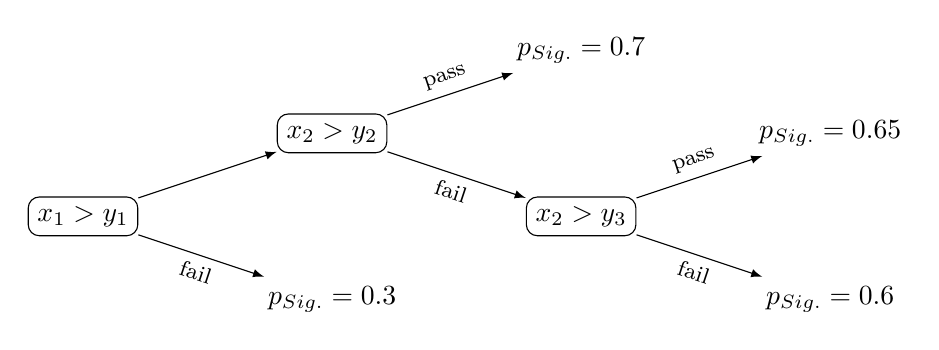
\begin{tikzpicture}
  [
    grow                    = right,
    sibling distance        = 6em,
    level distance          = 9em,
    edge from parent/.style = {draw, -latex,font=\footnotesize},
    sloped,
    treenode/.style = {shape=rectangle, rounded corners,
      draw, align=center},
    root/.style     = {treenode},
    env/.style      = {treenode},
    leaf/.style      = {treenode, draw=white}
  ]
  \node [root] {$x_{1} > y_{1}$}
    child { node [leaf] {$p_{\text{Sig.}} = 0.3$}
      edge from parent node [below] {fail} }
    child { node [env] {$x_{2} > y_{2}$}
      child { node [env] {$x_{2} > y_{3}$}
        child { node [leaf] {$p_{\text{Sig.}} = 0.6$}
          edge from parent node [below] {fail} }
        child { node [leaf] {$p_{\text{Sig.}} = 0.65$}
          edge from parent node [above] {pass} }
        edge from parent node [below] {fail} }
      child { node [leaf] {$p_{\text{Sig.}} = 0.7$}
        edge from parent node [above, align=center]
        {pass} }
    };
\end{tikzpicture}

  \caption{%
    A decision tree, computing signal probabilities $p_{\text{Sig.}}$ in the 
    leaf nodes using a set of features $x_{i}$ and cut values on those features 
    $y_{i}$.
  }
  \label{fig:cpv:kinematic_weighting:decision_tree}
\end{figure}

The construction, or growth, of a single decision tree is the process to 
determine which features and cut values are used in what nodes, and what the 
assigned probabilities should be in the terminal nodes.
There are many parameters available for tuning during construction, including: 
the maximum depth; the figure of merit the cut at each node should optimise; 
and the stopping criteria that determines whether additional nodes can be 
created.
Both tuning of these \emph{hyper-parameters} and of the features and cuts to 
use is a complex optimisation problem~\cite{Louppe:14077502}, the details of 
which are not necessary for understanding the classification problem at hand.
The important feature of the construction is that it is performed using an 
ensemble of individual \emph{events}, feature vectors $\vec{x}$, called the 
\emph{training} sample, in which the true species of each event is known.
This is typically a combination of some simulated \ac{MC} sample, known to be 
signal is known through truth-matching, and some sample from a control region 
in the data which is known to contain no signal, such as mass sidebands.
The decision tree then tries to fit the set of cuts and values such that the 
samples can be classified as cleanly as possible, given the hyper-parameters.
The probability of the terminal nodes can then be taken as, for example, the 
ratio of the two species that remain after the training sample has been passed 
through the final tree.

The discriminating power of a decision tree is driven by two factors: how 
discriminatory the set of features is between the two species; and what the 
values of the hyper-parameters are.
The exact choice of these is dependent on the nature of the classification 
problem, however the hyper-parameters should be chosen such that the decision 
tree is not \emph{over-fitted} to the training data.
This occurs when the tree is too sensitive to the statistical fluctuations in 
the features in the training sample.
It is possible that a tree with infinitely many layers would be able to 
perfectly classify the training sample, for example, but a new signal sample 
not present in the training may be classified as background, as the values of 
the features do not exactly match those in the training sample.
In general, over-fitting results in the performance of the tree being worse on 
an independent \emph{testing} sample, within which the true species are also 
known, than on the training sample.
When tuning the set of hyper-parameters, the performance of the tree should 
then be evaluated on the testing sample.
This is comparable with the normal fitting of functions to data with maximum 
likelihood or \chisq\ methods, in that more complex models can describe the 
data well, to an arbitrary degree for higher complexities, but the models begin 
to offer less general insight, instead being tailored to a specific dataset 
that happens to have been observed.
Measures of performance include the \emph{accuracy}, the number of correctly 
classified events relative to the total number, and the \emph{error rate}, the 
number of wrong predictions relative to the total number.
In the worst case, a classifier does no better at guessing event species than 
uniform random guessing.

The benefit of using decision trees over some other \ac{MVA} algorithms is that 
they can be intuitively interpreted: the tree can be visualised as such, and 
the decisions can be reasoned with by seeing how different features influence 
the lower depths of the tree.
However, a tree that fits the training sample well is in general very deep, as 
only one feature enters the decision in each node.
Deep trees are particularly susceptible to over-fitting, and so \emph{ensemble} 
methods are often used.

\subsection{Ensembles of trees and boosting}
\label{chap:cpv:kinematic_weighting:bdt_theory:ensembles}

The error rate of a decision tree, the fraction of incorrectly classified 
events, is due to two properties of the classifier: the bias, the consistent 
deviation away from the true values, and the variance, the spread around the 
mean value~\cite{Breiman96biasvariance}.
A complex model, prone to over-fitting, may have a low bias but a high 
variance, whereas a simple model may have a high bias but a low variance.

To reduce the variance of a tree-based classifier, ensembles of complex trees 
can be created, where each tree is grown using a subset of the training 
data~\cite{Breiman1996}.
The classification for an event is then determined using the set of 
classifications produced by the ensemble, such as by taking the mean of that 
set.
This does not increase the bias of the model if the predictions of the 
individual trees are uncorrelated.
To guard against this possibility, the technique of \emph{random 
  forests}~\cite{Breiman2001,Louppe:14077502} can be used, in which each node 
splitting can only use information from a random subset of the features, in 
addition to the random sub-sampling of the training data used to grow each tree 
in the ensemble.

The bias can be decreased by employing \emph{boosting}, for which 
\adaboost~\cite{Freund1997119} is commonly used algorithm.
Rather than training an ensemble of complex models in parallel, \adaboost\ 
trains a \emph{sequence} of \emph{weak learners} (decisions trees here), whose 
predictions are only slightly better than random guessing, and returns a 
weighted sum of their predictions as the final classification.
This begins by growing a single, shallow tree where the $i$th vector in the 
training sample is weighted with a weight $w_{i} = 1/N$.
The training sample is fed through the tree, and events which were classified 
incorrectly are assigned a larger weight, and those which were classified 
correctly are assigned a smaller weight.
A new tree is grown using the new weights, and the procedure is iterated.
With each iteration, events that are consistently incorrectly classified are 
given a greater importance in the training.

The generalisation of the \adaboost\ algorithm is \emph{gradient 
  boosting}~\cite{friedman2001}.
With \adaboost, additional weak learners compensate for previous incorrect 
classifications by being trained with specially weighted data.
In gradient boosting, additional weak learners try to correct the 
classification of the previous learners by fitting a regression model 
$f(\vec{x})$ to the residuals ${(\hat{y}_{i} - f(\vec{x}_{i}))}^2$ of the 
predicted classification $f(\vec{x}_{i}) = y_{i}$ and the true classification 
$\hat{y}_{i}$.
In this way, gradient boosting tries to minimise the \emph{loss function} that 
characterises how poorly the classifier is performing, and can be generalised 
by considering an arbitrary loss function $L(\hat{y}, f(x))$, which can be the 
residual.

\section{Weighting with decision trees}
\label{chap:cpv:kinematic_weighting:bdt_method}

It is common in \acl{HEP} to want to be able to bring two distributions into 
agreement, as is the case in this analysis where particle kinematics should be 
equal between the \pKK\ and \ppipi\ data.
Call one possibly multi-dimensional distribution the \emph{target} $f_{t}$ and 
the other the \emph{original} distribution $f_{o}$.
To transform $f_{o}$ to have the same form as $f_{t}$, there is some 
transformation function $W$
\begin{equation}
  f_{t}(x) = W(x)f_{o}(x),
\end{equation}
where $x$ is a possibly multi-dimensional parameter.
As the true distributions of $f_{t}$ and $f_{o}$ are not known in the data, 
they are approximated as histograms, partitioning the data in $x$ and counting 
the number of events that fall in each bin.
The transformation function is quantised as $w$ in bins, where in the $i$th bin
\begin{equation}
  f_{t}(x_{i}) = w(x_{i})f_{o}(x_{i}),
\end{equation}
and where $f_{t(o)}(x_{i})$ is the count of the target (original) distribution 
in the $i$th bin.
The histogram of $f_{o}$ can be transformed to that of $f_{t}$ by computing the 
per-bin \emph{weights}
\begin{equation}
  w(x_{i}) = \frac{f_{t}(x_{i})}{f_{o}(x_{i})}.
\end{equation}
This is valid assuming there are no bins where $f_{o}(x_{i}) = 0$.

To model the true \aclp{PDF} in $x$ as closely as possible, the histogram must 
have a fine enough binning that all structures are resolved.
Specifically, as in the determination of the \ac{PID} efficiency in 
\cref{chap:prod:effs:pid}, the binning must be fine enough such that difference 
between the true \acp{PDF} of the two distribution within any given bin are 
small.
This must be balanced with the limited statistical precision available in each 
bin: too fine a binning will result in the original distribution being weighted 
to match the statistical fluctuations in the target, rather than the physical 
features.
Limited sample sizes become particularly problematic for higher-dimensional 
weighting, when even 10 equally spaced bins per dimension in a 
three-dimensional binning requires $1,000$ bins.
Given physical distributions such as momentum and pseudorapidity, which have 
long tails, it can be difficult to invent a binning that avoids sparsely 
populated or empty bins whilst still accounting for differences in the 
distributions.

To overcome the limitations of histogram-based weighting, this analysis defers 
the computation of the per-event weights $w_{i}$ to a decision tree with 
gradient boosting~\cite{Rogozhnikov:2016bdp}.
The classifier is trained as in the gradient boosting method described in 
\cref{chap:cpv:kinematic_weighting:bdt_theory}, with the loss function
\begin{equation}
  L = \sum_{l \in \text{Leaves}} \frac{%
    {(w_{l,o} - w_{l,t})}^{2}
  }{%
    w_{l,o} + w_{l,t}
  },
\end{equation}
where $w_{l,t(o)}$ is the sum of target (original) weights in the $l$th leaf 
node of the regression tree.
For the initial iteration, and an unweighted set of training events, this is 
equal to the number of target (original) events in the leaf node.
This metric has the tree split the samples into regions where the differences 
between the sample sizes is maximal, and is chosen because these are the 
regions with the largest differences, and so the classifier should focus on 
weighting them.
Predictions $p_{l}$ within a leaf are computed as
\begin{equation}
  p_{l} = \log{\frac{w_{l,t}}{w_{l,o}}}.
\end{equation}
At the end of the $i$th iteration, each event from the `original' sample is 
weighted by $w_{i} = w_{i - 1}e^{p_{l}}$, where $l$ is the leaf node the event 
falls in.
The target distribution is assigned unit weights $w_{i} = w_{0}$.
This weighting has the same effect as the weighting in the \adaboost\ 
algorithm, increasing the importance of events in the original distribution 
that are in regions with a large original/target difference.

The actual weighting of events is identical to that in the histogram weighting: 
it is the ratio of target to original events in some region.
The use of gradient boosting allows for a more intelligent way of finding the 
`bins' in which the weights are computed, and iteratively improves the weights 
based on that method.

\section{Evaluation}
\label{chap:cpv:kinematic_weighting:evaluation}

The decision tree with gradient boosting is trained with the \ppipi\ data as 
the `original' sample and the \pKK\ data as the `target'.
The weighting procedure is performed separately for each data sub-sample in 
year and magnet polarity.
As it is expected that the \PLambdab\ and muon kinematics are correlated with 
that of the \PLambdac, the \PLambdac\ transverse momentum \pT\ and 
pseudorapidity \Eta\ are included as inputs to the \ac{BDT}.
Also included are the proton \pT\ and \Eta, as these distributions are seen to 
disagree after weighting when only the \PLambdac\ kinematics are used.
To avoid biases due to fluctuations in the data, two classifiers $A$ and $B$ 
are trained, and the \pKK\ and \ppipi\ data are each randomly split into two 
sub-samples 1 and 2: classifier $A$ is trained using sub-sample 1, and the 
weights for sub-sample 2 are computed using $A$; likewise, classifier $B$ is 
trained using sub-sample 2, and the weights for sub-sample 1 are computed using 
$B$.
Sub-samples 1 and 2 are then combined for the remainder of the analysis.
The input training data are weighted by signal sWeights, as computed from the 
result of the mass fits described in \cref{chap:cpv:prelim_fits}.
Each classifier is boosted in 300 iterations, the maximum number of leaf nodes 
allow in the regression tree is four, and the criteria for splitting includes 
the requirement that any new nodes must contain at least 200 events.
The choice of these hyper-parameters will be discussed in 
\cref{chap:cpv:kinematic_weighting:validation}, as well as the specific choice 
of original and target samples.

\Cref{fig:cpv:kinematic_weighting:post:Lb,fig:cpv:kinematic_weighting:post:Lb_mu,fig:cpv:kinematic_weighting:post:Lc,fig:cpv:kinematic_weighting:post:Lc_p} 
show the \PLambdab, muon, \PLambdac, and proton kinematics after weighting with 
the product of signal sWeights and the kinematic weights.
\Cref{fig:cpv:kinematic_weighting:post:pKK_h1h2,fig:cpv:kinematic_weighting:post:ppipi_h1h2} 
show the $\Phm\Php$ kinematics, \emph{within} the modes, after the same 
weighting.
There is a considerable improvement in the agreement between the \pKK\ and 
\ppipi\ data in the \PLambdab\ and proton kinematics.
The good agreement in the muon kinematics between the datasets and the 
$\Phm\Phm$ kinematics within the datasets does not change,
It is noted that the \PLambdac\ kinematic agreement also improves, although 
this does not affect the measurement of \dACP\ as there is no associated 
asymmetry.

\section{Validation}
\label{chap:cpv:kinematic_weighting:validation}

The purpose of the kinematic weighting is to make the particle kinematics 
indistinguishable between the \pKK\ and \ppipi\ modes.
\Cref{fig:cpv:kinematic_weighting:post:Lb,fig:cpv:kinematic_weighting:post:Lb_mu,fig:cpv:kinematic_weighting:post:Lc,fig:cpv:kinematic_weighting:post:Lc_p} 
show good agreement `by eye', but a quantitative assessment is needed.
What affects the measurement of \dACP\ is not so much the absolute level of 
disagreement the two histograms, for example, but the disagreement in a 
particular region combined with both the size of the respective asymmetries 
involved and the density of the data in that region.
The effect of the remaining differences on \dACP\ is discussed in the context 
of systematic uncertainties in \cref{chap:cpv:syst}.

To provide some quantitative estimate of the agreement, a \ac{BDT} is employed.
If the two samples, the target weighted with signal sWeights and the original 
weighted with the product of signal sWeights and kinematic weights, are truly 
identical, then a \ac{BDT} designed to \emph{discriminate} between them should 
perform no better than random guessing.
The performance of a \ac{BDT} trained for binary classification can be 
evaluated by computing the area under the \ac{ROC} curve, or just \ac{AUC}.
The \ac{ROC} curve compares the \ac{FPR} of the classifier with the \ac{TPR} as 
a function of the classifier output probability.
The \ac{TPR} is defined as the fraction of true signal events that are 
correctly classified as such, whilst the \ac{FPR} is the fraction of background 
events that are classified as signal.
Plotting the \ac{FPR} increasing along the $x$-axis and the \ac{TPR} increasing 
along the $y$-axis, the \ac{ROC} curve for an optimal classifier passes through 
the top-left corner of the plot, where a large fraction of the signal is 
accepted and a correspondingly large background fraction is rejected.
A classifier that cannot distinguish between signal and background any better 
than random guessing will have a \ac{ROC} curve of the form $x = y$.
In these two extreme cases, the \ac{AUC} is 1 and 0.5, respectively.

A \ac{BDT}, with gradient boosting, is trained to discriminate between the 
weighted \pKK\ and \ppipi\ data, using three-quarters of the available 2012 
magnet down data as input.
The \PLambdab, muon, and proton \ptot, \pT, \Eta, and azimuthal angle $\phi$ 
are used as features.
The \PLambdac\ kinematics are not included as there is no asymmetry associated 
to any residual differences there might be.
The maximum number of leaf nodes for any one regression tree is 11, the number 
of boosting iterations performed is 400, and the minimum number of samples 
allowed in a leaf node is 200.
The performance of the \ac{BDT} is evaluated using the remaining quarter of the 
dataset, and the resulting \ac{ROC} curve is shown in 
\cref{fig:cpv:kinematic_weighting:post:roc}.
For comparison, it is shown along with a curve obtained when the same 
classifier is trained using data with no kinematic weighting, as well as a 
curve when a rudimentary, two-dimensional, $10\times10$ histogram weighting in 
\PLambdac\ \pT\ and \Eta\ is used.
It is seen that the inclusion of the kinematic weights significantly reduces 
the \ac{AUC}, from 0.61 with no kinematic weights to 0.52 for the \ac{BDT} 
weighting.
This shows that the \ac{BDT} weighting does increase the similarity between the 
kinematic distributions across the modes, and that it can be significantly more 
powerful than a two-dimensional histogram weighting.

It is the \ac{AUC} metric evaluated on the training sample that was maximised 
when choosing the hyper-parameters to use for the weighting.
A grid search was performed where the following hyper-parameter values were 
tested in all combinations: 100, 200, 300, and 400 boosting iterations; a 
minimum of 50, 100, 200, 300, 500, and 1000 events required to create a new 
node; and a maximum number of allowed leaf nodes per regression tree of 2, 3, 
4, 5, 6, 7, and 8.
The hyper-parameters used for the weighting (300 iterations, a minimum of 200 
events per node, and a maximum of 4 leaf nodes per tree) were those for which 
the \ac{AUC} was smallest.

\section{Weight statistics}
\label{chap:cpv:kinematic_weighting:stats}

Weighting can increase the statistical contribution of individual entries 
within a dataset, but it should not increase the overall statistical power.
The number of entries $N'$ in a weighted dataset can be computed as the sum of 
the per-entry weights $w_{i}$, and the variance on this quantity is given as 
the sum of the squares of the weights
\begin{equation}
  N' = \sum_{i}^{N} w_{i},\quad (\unc{N'})^{2} = \sum_{i}^{N} w_{i}^{2}
\end{equation}
For certain values of $w_{i}$, it can be that $\unc{N'} < \unc{N}$.
To prevent this, the number of `effective' entries in the weighted dataset is 
computed, under the relation that the relative variance on the effective 
entries is equal to the relative variance on the weights
\begin{equation}
  \frac{\neff}{\unc{\neff}} =
    \frac{\sum_{i}^{N} w_{i}}{\sqrt{\sum_{i}^{N} w_{i}^{2}}},
\end{equation}
where \neff\ is assumed to be Poisson-distributed, and so $(\unc{\neff})^{2} = 
\neff$, giving
\begin{equation}
  \neff = \frac{%
    {\left(\sum_{i}^{N}{w_{i}}\right)}^{2}
  }{%
    \sum_{i}^{N}{w_{i}^{2}},
  }.
  \label{eqn:cpv:kinematic_weighting:neff}
\end{equation}
This relation can be enforced by redefining the weights $w_{i}$ by a factor $W 
= \sum_{i} w_{i}/\sum_{i} w_{i}^{2}$.
For unit weights, $\neff = N$ add $\unc{\neff} = \sqrt{N}$.
Otherwise, \neff\ is the size of the hypothetical dataset that has the same 
statistical power as the weighted dataset.
For this analysis, it provides a handle on how well the two data samples agree 
in the weighting variables before the weighting, as, in general, a higher level 
of disagreement requires a larger fraction of candidates to be `thrown away' by 
the weighting, reducing the statistical power.

\Cref{tab:cpv:kinematic_weighting:validation:stats} gives several statistics 
related to the weighting procedure.
The statistics relate to the \ppipi\ data, as it is that which is weighted.
For all data sub-samples, the effective number of candidates is no less than 
\SI{80}{\percent} the number of candidates entering the weighting procedure.
As there are around five times more \ppipi\ candidates than \pKK, the 
statistical uncertainty of the \dACP\ measurement will still be dominated by 
the \pKK\ sample size, even with an effective \SI{20}{\percent} reduction in 
the \ppipi\ sample size.
It is this fact that motivates the choice of the \ppipi\ mode as the source of 
the `original' distributions in the weighting and the \pKK\ mode as the 
`target'.

\begin{sidewaystable}
  \centering
  \caption{%
    Statistics computed on the weighted \ppipi\ data for all data sub-samples 
    used in the analysis.
    The quantities are defined in \cref{chap:cpv:kinematic_weighting:stats}.
  }
  \label{tab:cpv:kinematic_weighting:validation:stats}
  \begin{tabular}{ccccccccc}
  \toprule
  Year & Polarity & $N$    & $\sum{w_{i}}$ & $\sum{w_{i}^{2}}$ & $\sqrt{\sum{w_{i}^{2}}}$ & \neff  & $\unc{\neff}$ & $\frac{\neff}{N}$ \\
  \midrule
  2011   & Up       & 42688  & 39408         & 44801             & 211                      & 34663  & 186           & 0.812             \\
  2011   & Down     & 59044  & 53627         & 58867             & 242                      & 48853  & 221           & 0.827             \\
  2012   & Up       & 147064 & 137461        & 155696            & 394                      & 121362 & 348           & 0.825             \\
  2012   & Down     & 148218 & 138168        & 153675            & 392                      & 124227 & 352           & 0.838             \\
  \bottomrule
\end{tabular}

\end{sidewaystable}

\clearpage

\begin{figure}
  \begin{subfigure}[b]{0.4\textwidth}
    \includegraphics[width=\textwidth]{cpv/kinematic_weighting/preweighting_kinematics/LcToppipi_2012_MagDown_Lb_P}
    \label{fig:cpv:kinematic_weighting:pre:Lb:P}
  \end{subfigure}
  \begin{subfigure}[b]{0.4\textwidth}
    \includegraphics[width=\textwidth]{cpv/kinematic_weighting/preweighting_kinematics/LcToppipi_2012_MagDown_Lb_PT}
    \label{fig:cpv:kinematic_weighting:pre:Lb:PT}
  \end{subfigure}\\
  \begin{subfigure}[b]{0.4\textwidth}
    \includegraphics[width=\textwidth]{cpv/kinematic_weighting/preweighting_kinematics/LcToppipi_2012_MagDown_Lb_ETA}
    \label{fig:cpv:kinematic_weighting:pre:Lb:ETA}
  \end{subfigure}
  \begin{subfigure}[b]{0.4\textwidth}
    \includegraphics[width=\textwidth]{cpv/kinematic_weighting/preweighting_kinematics/LcToppipi_2012_MagDown_Lb_PHI}
    \label{fig:cpv:kinematic_weighting:pre:Lb:PHI}
  \end{subfigure}
  \caption{%
    Clockwise from the top left: total momentum, transverse momentum, angle 
    $\phi$, and pseudorapidity of the \PLambdab, weighted by signal sWeights.
    The 2012 magnet down data is shown.
  }
  \label{fig:cpv:kinematic_weighting:pre:Lb}
\end{figure}

\begin{figure}
  \begin{subfigure}[b]{0.4\textwidth}
    \includegraphics[width=\textwidth]{cpv/kinematic_weighting/preweighting_kinematics/LcToppipi_2012_MagDown_Lb_mu_P}
    \label{fig:cpv:kinematic_weighting:pre:Lb_mu:P}
  \end{subfigure}
  \begin{subfigure}[b]{0.4\textwidth}
    \includegraphics[width=\textwidth]{cpv/kinematic_weighting/preweighting_kinematics/LcToppipi_2012_MagDown_Lb_mu_PT}
    \label{fig:cpv:kinematic_weighting:pre:Lb_mu:PT}
  \end{subfigure}\\
  \begin{subfigure}[b]{0.4\textwidth}
    \includegraphics[width=\textwidth]{cpv/kinematic_weighting/preweighting_kinematics/LcToppipi_2012_MagDown_Lb_mu_ETA}
    \label{fig:cpv:kinematic_weighting:pre:Lb_mu:ETA}
  \end{subfigure}
  \begin{subfigure}[b]{0.4\textwidth}
    \includegraphics[width=\textwidth]{cpv/kinematic_weighting/preweighting_kinematics/LcToppipi_2012_MagDown_Lb_mu_PHI}
    \label{fig:cpv:kinematic_weighting:pre:Lb_mu:PHI}
  \end{subfigure}
  \caption{%
    Clockwise from the top left: total momentum, transverse momentum, angle 
    $\phi$, and pseudorapidity of the muon from the \PLambdab, weighted by 
    signal sWeights.
    The 2012 magnet down data is shown.
  }
  \label{fig:cpv:kinematic_weighting:pre:Lb_mu}
\end{figure}

\begin{figure}
  \begin{subfigure}[b]{0.4\textwidth}
    \includegraphics[width=\textwidth]{cpv/kinematic_weighting/preweighting_kinematics/LcToppipi_2012_MagDown_Lc_P}
    \label{fig:cpv:kinematic_weighting:pre:Lc:P}
  \end{subfigure}
  \begin{subfigure}[b]{0.4\textwidth}
    \includegraphics[width=\textwidth]{cpv/kinematic_weighting/preweighting_kinematics/LcToppipi_2012_MagDown_Lc_PT}
    \label{fig:cpv:kinematic_weighting:pre:Lc:PT}
  \end{subfigure}\\
  \begin{subfigure}[b]{0.4\textwidth}
    \includegraphics[width=\textwidth]{cpv/kinematic_weighting/preweighting_kinematics/LcToppipi_2012_MagDown_Lc_ETA}
    \label{fig:cpv:kinematic_weighting:pre:Lc:ETA}
  \end{subfigure}
  \begin{subfigure}[b]{0.4\textwidth}
    \includegraphics[width=\textwidth]{cpv/kinematic_weighting/preweighting_kinematics/LcToppipi_2012_MagDown_Lc_PHI}
    \label{fig:cpv:kinematic_weighting:pre:Lc:PHI}
  \end{subfigure}
  \caption{%
    Clockwise from the top left: total momentum, transverse momentum, angle 
    $\phi$, and pseudorapidity of the \PLambdac, weighted by signal sWeights.
    The 2012 magnet down data is shown.
  }
  \label{fig:cpv:kinematic_weighting:pre:Lc}
\end{figure}

\begin{figure}
  \begin{subfigure}[b]{0.4\textwidth}
    \includegraphics[width=\textwidth]{cpv/kinematic_weighting/preweighting_kinematics/LcToppipi_2012_MagDown_Lc_p_P}
    \label{fig:cpv:kinematic_weighting:pre:Lc_p:P}
  \end{subfigure}
  \begin{subfigure}[b]{0.4\textwidth}
    \includegraphics[width=\textwidth]{cpv/kinematic_weighting/preweighting_kinematics/LcToppipi_2012_MagDown_Lc_p_PT}
    \label{fig:cpv:kinematic_weighting:pre:Lc_p:PT}
  \end{subfigure}\\
  \begin{subfigure}[b]{0.4\textwidth}
    \includegraphics[width=\textwidth]{cpv/kinematic_weighting/preweighting_kinematics/LcToppipi_2012_MagDown_Lc_p_ETA}
    \label{fig:cpv:kinematic_weighting:pre:Lc_p:ETA}
  \end{subfigure}
  \begin{subfigure}[b]{0.4\textwidth}
    \includegraphics[width=\textwidth]{cpv/kinematic_weighting/preweighting_kinematics/LcToppipi_2012_MagDown_Lc_p_PHI}
    \label{fig:cpv:kinematic_weighting:pre:Lc_p:PHI}
  \end{subfigure}
  \caption{%
    Clockwise from the top left: total momentum, transverse momentum, angle 
    $\phi$, and pseudorapidity of the proton from the \PLambdac, weighted by 
    signal sWeights.
    The 2012 magnet down data is shown.
  }
  \label{fig:cpv:kinematic_weighting:pre:Lc_p}
\end{figure}

\begin{figure}
  \begin{subfigure}[b]{0.5\textwidth}
    \centering
    \includegraphics[width=0.8\textwidth]{cpv/kinematic_weighting/preweighting_kinematics/LcToppipi_2012_MagDown_h1_h2_P_LcTopKK}
    \label{fig:cpv:kinematic_weighting:pre:pKK_h1h2:P}
  \end{subfigure}
  \begin{subfigure}[b]{0.5\textwidth}
    \centering
    \includegraphics[width=0.8\textwidth]{cpv/kinematic_weighting/preweighting_kinematics/LcToppipi_2012_MagDown_h1_h2_PT_LcTopKK}
    \label{fig:cpv:kinematic_weighting:pre:pKK_h1h2:PT}
  \end{subfigure}\\
  \begin{subfigure}[b]{\textwidth}
    \centering
    \includegraphics[width=0.4\textwidth]{cpv/kinematic_weighting/preweighting_kinematics/LcToppipi_2012_MagDown_h1_h2_ETA_LcTopKK}
    \label{fig:cpv:kinematic_weighting:pre:pKK_h1h2:ETA}
  \end{subfigure}
  \caption{%
    Clockwise from the top left: total momentum, transverse momentum, and 
    pseudorapidity of the \PKminus\ and \PKplus\ \PLambdac\ children in the 
    \pKK\ data, weighted by signal sWeights.
    The 2012 magnet down data is shown.
  }
  \label{fig:cpv:kinematic_weighting:pre:pKK_h1h2}
\end{figure}

\begin{figure}
  \begin{subfigure}[b]{0.5\textwidth}
    \centering
    \includegraphics[width=0.8\textwidth]{cpv/kinematic_weighting/preweighting_kinematics/LcToppipi_2012_MagDown_h1_h2_P_LcToppipi}
    \label{fig:cpv:kinematic_weighting:pre:ppipi_h1h2:P}
  \end{subfigure}
  \begin{subfigure}[b]{0.5\textwidth}
    \centering
    \includegraphics[width=0.8\textwidth]{cpv/kinematic_weighting/preweighting_kinematics/LcToppipi_2012_MagDown_h1_h2_PT_LcToppipi}
    \label{fig:cpv:kinematic_weighting:pre:ppipi_h1h2:PT}
  \end{subfigure}\\
  \begin{subfigure}[b]{\textwidth}
    \centering
    \includegraphics[width=0.4\textwidth]{cpv/kinematic_weighting/preweighting_kinematics/LcToppipi_2012_MagDown_h1_h2_ETA_LcToppipi}
    \label{fig:cpv:kinematic_weighting:pre:ppipi_h1h2:ETA}
  \end{subfigure}
  \caption{%
    Clockwise from the top left: total momentum, transverse momentum, and 
    pseudorapidity of the \Ppiminus\ and \Ppiplus\ \PLambdac\ children in the 
    \ppipi\ data, weighted by signal sWeights.
    The 2012 magnet down data is shown.
  }
  \label{fig:cpv:kinematic_weighting:pre:ppipi_h1h2}
\end{figure}

\begin{figure}
  \begin{subfigure}[b]{0.4\textwidth}
    \includegraphics[width=\textwidth]{cpv/kinematic_weighting/postweighting_kinematics/LcToppipi_2012_MagDown_Lb_P-weighted}
    \label{fig:cpv:kinematic_weighting:post:Lb:P}
  \end{subfigure}
  \begin{subfigure}[b]{0.4\textwidth}
    \includegraphics[width=\textwidth]{cpv/kinematic_weighting/postweighting_kinematics/LcToppipi_2012_MagDown_Lb_PT-weighted}
    \label{fig:cpv:kinematic_weighting:post:Lb:PT}
  \end{subfigure}\\
  \begin{subfigure}[b]{0.4\textwidth}
    \includegraphics[width=\textwidth]{cpv/kinematic_weighting/postweighting_kinematics/LcToppipi_2012_MagDown_Lb_ETA-weighted}
    \label{fig:cpv:kinematic_weighting:post:Lb:ETA}
  \end{subfigure}
  \begin{subfigure}[b]{0.4\textwidth}
    \includegraphics[width=\textwidth]{cpv/kinematic_weighting/postweighting_kinematics/LcToppipi_2012_MagDown_Lb_PHI-weighted}
    \label{fig:cpv:kinematic_weighting:post:Lb:PHI}
  \end{subfigure}
  \caption{%
    Clockwise from the top left: total momentum, transverse momentum, angle 
    $\phi$, and pseudorapidity of the \PLambdab, weighted by the product of 
    signal sWeights and kinematic weights.
    The 2012 magnet down data is shown.
  }
  \label{fig:cpv:kinematic_weighting:post:Lb}
\end{figure}

\begin{figure}
  \begin{subfigure}[b]{0.4\textwidth}
    \includegraphics[width=\textwidth]{cpv/kinematic_weighting/postweighting_kinematics/LcToppipi_2012_MagDown_Lb_mu_P-weighted}
    \label{fig:cpv:kinematic_weighting:post:Lb_mu:P}
  \end{subfigure}
  \begin{subfigure}[b]{0.4\textwidth}
    \includegraphics[width=\textwidth]{cpv/kinematic_weighting/postweighting_kinematics/LcToppipi_2012_MagDown_Lb_mu_PT-weighted}
    \label{fig:cpv:kinematic_weighting:post:Lb_mu:PT}
  \end{subfigure}\\
  \begin{subfigure}[b]{0.4\textwidth}
    \includegraphics[width=\textwidth]{cpv/kinematic_weighting/postweighting_kinematics/LcToppipi_2012_MagDown_Lb_mu_ETA-weighted}
    \label{fig:cpv:kinematic_weighting:post:Lb_mu:ETA}
  \end{subfigure}
  \begin{subfigure}[b]{0.4\textwidth}
    \includegraphics[width=\textwidth]{cpv/kinematic_weighting/postweighting_kinematics/LcToppipi_2012_MagDown_Lb_mu_PHI-weighted}
    \label{fig:cpv:kinematic_weighting:post:Lb_mu:PHI}
  \end{subfigure}
  \caption{%
    Clockwise from the top left: total momentum, transverse momentum, angle 
    $\phi$, and pseudorapidity of the muon from the \PLambdab, weighted by the 
    product of signal sWeights and kinematic weights.
    The 2012 magnet down data is shown.
  }
  \label{fig:cpv:kinematic_weighting:post:Lb_mu}
\end{figure}

\begin{figure}
  \begin{subfigure}[b]{0.4\textwidth}
    \includegraphics[width=\textwidth]{cpv/kinematic_weighting/postweighting_kinematics/LcToppipi_2012_MagDown_Lc_P-weighted}
    \label{fig:cpv:kinematic_weighting:post:Lc:P}
  \end{subfigure}
  \begin{subfigure}[b]{0.4\textwidth}
    \includegraphics[width=\textwidth]{cpv/kinematic_weighting/postweighting_kinematics/LcToppipi_2012_MagDown_Lc_PT-weighted}
    \label{fig:cpv:kinematic_weighting:post:Lc:PT}
  \end{subfigure}\\
  \begin{subfigure}[b]{0.4\textwidth}
    \includegraphics[width=\textwidth]{cpv/kinematic_weighting/postweighting_kinematics/LcToppipi_2012_MagDown_Lc_ETA-weighted}
    \label{fig:cpv:kinematic_weighting:post:Lc:ETA}
  \end{subfigure}
  \begin{subfigure}[b]{0.4\textwidth}
    \includegraphics[width=\textwidth]{cpv/kinematic_weighting/postweighting_kinematics/LcToppipi_2012_MagDown_Lc_PHI-weighted}
    \label{fig:cpv:kinematic_weighting:post:Lc:PHI}
  \end{subfigure}
  \caption{%
    Clockwise from the top left: total momentum, transverse momentum, angle 
    $\phi$, and pseudorapidity of the \PLambdac, weighted by the product of 
    signal sWeights and kinematic weights.
    The 2012 magnet down data is shown.
  }
  \label{fig:cpv:kinematic_weighting:post:Lc}
\end{figure}

\begin{figure}
  \begin{subfigure}[b]{0.4\textwidth}
    \includegraphics[width=\textwidth]{cpv/kinematic_weighting/postweighting_kinematics/LcToppipi_2012_MagDown_Lc_p_P-weighted}
    \label{fig:cpv:kinematic_weighting:post:Lc_p:P}
  \end{subfigure}
  \begin{subfigure}[b]{0.4\textwidth}
    \includegraphics[width=\textwidth]{cpv/kinematic_weighting/postweighting_kinematics/LcToppipi_2012_MagDown_Lc_p_PT-weighted}
    \label{fig:cpv:kinematic_weighting:post:Lc_p:PT}
  \end{subfigure}\\
  \begin{subfigure}[b]{0.4\textwidth}
    \includegraphics[width=\textwidth]{cpv/kinematic_weighting/postweighting_kinematics/LcToppipi_2012_MagDown_Lc_p_ETA-weighted}
    \label{fig:cpv:kinematic_weighting:post:Lc_p:ETA}
  \end{subfigure}
  \begin{subfigure}[b]{0.4\textwidth}
    \includegraphics[width=\textwidth]{cpv/kinematic_weighting/postweighting_kinematics/LcToppipi_2012_MagDown_Lc_p_PHI-weighted}
    \label{fig:cpv:kinematic_weighting:post:Lc_p:PHI}
  \end{subfigure}
  \caption{%
    Clockwise from the top left: total momentum, transverse momentum, angle 
    $\phi$, and pseudorapidity of the proton from the \PLambdac, weighted by 
    the product of signal sWeights and kinematic weights.
    The 2012 magnet down data is shown.
  }
  \label{fig:cpv:kinematic_weighting:post:Lc_p}
\end{figure}

\begin{figure}
  \begin{subfigure}[b]{0.5\textwidth}
    \centering
    \includegraphics[width=0.8\textwidth]{cpv/kinematic_weighting/postweighting_kinematics/LcToppipi_2012_MagDown_h1_h2_P_LcTopKK-weighted}
    \label{fig:cpv:kinematic_weighting:post:pKK_h1h2:P}
  \end{subfigure}
  \begin{subfigure}[b]{0.5\textwidth}
    \centering
    \includegraphics[width=0.8\textwidth]{cpv/kinematic_weighting/postweighting_kinematics/LcToppipi_2012_MagDown_h1_h2_PT_LcTopKK-weighted}
    \label{fig:cpv:kinematic_weighting:post:pKK_h1h2:PT}
  \end{subfigure}\\
  \begin{subfigure}[b]{\textwidth}
    \centering
    \includegraphics[width=0.4\textwidth]{cpv/kinematic_weighting/postweighting_kinematics/LcToppipi_2012_MagDown_h1_h2_ETA_LcTopKK-weighted}
    \label{fig:cpv:kinematic_weighting:post:pKK_h1h2:ETA}
  \end{subfigure}
  \caption{%
    Clockwise from the top left: total momentum, transverse momentum, and 
    pseudorapidity of the \PKminus\ and \PKplus\ \PLambdac\ children in the 
    \pKK\ data, weighted by the product of signal sWeights and kinematic 
    weights.
    The 2012 magnet down data is shown.
  }
  \label{fig:cpv:kinematic_weighting:post:pKK_h1h2}
\end{figure}

\begin{figure}
  \begin{subfigure}[b]{0.5\textwidth}
    \centering
    \includegraphics[width=0.8\textwidth]{cpv/kinematic_weighting/postweighting_kinematics/LcToppipi_2012_MagDown_h1_h2_P_LcToppipi-weighted}
    \label{fig:cpv:kinematic_weighting:post:ppipi_h1h2:P}
  \end{subfigure}
  \begin{subfigure}[b]{0.5\textwidth}
    \centering
    \includegraphics[width=0.8\textwidth]{cpv/kinematic_weighting/postweighting_kinematics/LcToppipi_2012_MagDown_h1_h2_PT_LcToppipi-weighted}
    \label{fig:cpv:kinematic_weighting:post:ppipi_h1h2:PT}
  \end{subfigure}\\
  \begin{subfigure}[b]{\textwidth}
    \centering
    \includegraphics[width=0.4\textwidth]{cpv/kinematic_weighting/postweighting_kinematics/LcToppipi_2012_MagDown_h1_h2_ETA_LcToppipi-weighted}
    \label{fig:cpv:kinematic_weighting:post:ppipi_h1h2:ETA}
  \end{subfigure}
  \caption{%
    Clockwise from the top left: total momentum, transverse momentum, and 
    pseudorapidity of the \Ppiminus\ and \Ppiplus\ \PLambdac\ children in the 
    \ppipi\ data, weighted by the product of signal sWeights and kinematic 
    weights.
    The 2012 magnet down data is shown.
  }
  \label{fig:cpv:kinematic_weighting:post:ppipi_h1h2}
\end{figure}

\begin{figure}
  \includegraphics[width=\textwidth]{cpv/kinematic_weighting/postweighting_kinematics/LcToppipi_2012_MagDown_roc_curves}
  \caption{%
    ROC curves for different kinematic weighting techniques.
    The ``no weights'' data has no \emph{kinematic} weights applied, only 
    signal sWeights.
    The ``2D binned'' and ``\ac{BDT}'' data uses the product of the respective 
    kinematic weights and the signal sWeights for the \ppipi\ data, and uses
    signal sWeights for the \pKK\ data.
    The area under each \ac{ROC} curve, the \acs{AUC}, is given in the legend.
  }
  \label{fig:cpv:kinematic_weighting:post:roc}
\end{figure}


\cleardoublepage

\appendix

\appendixpage*

% \chapter{Derivation of complicated equation}
\label{chap:derivation}

\lipsum[1-2].


\backmatter

\chapter{Acronyms}

\begin{acronym}
  \acro{QCD}{quantum chromodynamics}
  \acro{EM}{electromagnetic}
  \acro{EW}{electroweak}
  \acro{SM}{standard model}
  \acro{BSM}{beyond the \acl{SM}}
  \acro{CF}{Cabibbo-favoured}
  \acro{SCS}{singly Cabibbo-suppressed}
  \acro{DCS}{doubly Cabibbo-suppressed}

  \acro{QCDPDF}[PDF]{parton density function}
  \acro{DGLAP}{Dokshitzer-Gribov-Lipatov-Altarelli-Parisi}
  \acro{DIS}{deep inelastic scattering}
  \acro{\fonll}{fixed-order next-to-leading logarithms}
  \acro{\gmvfns}{generalised-mass variable-flavour-numbering scheme}

  \acro{MC}{Monte Carlo}
  \acro{PDF}{probability density function}
  \acro{MVA}{multivariate analysis}
  \acro{BDT}{boosted decision tree}
  \acro{KDE}{kernel density estimate}

  \acro{PV}{primary vertex}
  \acro{IP}{impact parameter}
  \acro{DOCA}{distance of closest approach}
  \acro{DIRA}{direction angle}
  \acro{DLL}{delta-log-likelihood}
  \acro{PID}{particle identification}

  \acro{L0}{level-zero}
  \acro{HLT}{high level trigger}

  \acro{LHC}{Large Hadron Collider}
  \acro{LS1}{\lsone}
  \acro{LHCIP}[IP]{interaction point}
  \acro{GPD}{general purpose detector}

  \acro{VDM}{van der Meer}
  \acro{BGI}{beam-gas imaging}

  \acro{PDG}{Particle Data Group}
\end{acronym}


\bibliographystyle{thesis}
\renewcommand{\bibname}{References}
\bibliography{bibliography}

\end{document}
